\documentclass[oneside]{book}
\usepackage{amsmath, amssymb, amsthm}
\usepackage{eso-pic}
\usepackage{graphicx}
\usepackage{subcaption}
\usepackage{hyperref}
\usepackage{euscript}
\usepackage{mathrsfs}
\usepackage{soul}
\usepackage[normalem]{ulem}
\usepackage{ctex}
\usepackage{tikz}
\usepackage{fancyhdr} % 用于自定义页眉页脚
\usepackage{lipsum}
\usepackage{transparent}
\usepackage[absolute,overlay]{textpos}
\usepackage{geometry}
\usepackage{cancel}
\usepackage{enumitem}
\usetikzlibrary{positioning}
% 双面排版：右侧页左边距3cm，左侧页右边距3cm，上下边距2.5cm
\geometry{a4paper, left=3cm, right=3cm, top=2.5cm, bottom=2.5cm}
\AddToShipoutPictureBG*{%
	\AtPageLowerLeft{%
		\transparent{0.6}% 透明度：0.3（0-1之间）
		\includegraphics[
		width=\paperwidth,
		height=\paperheight
		]{background.jpg}% 你的图片路径
	}%
}
\title{离散数学/组合数学\\Discrete Mathematics\\ and \\ Combinatorics}
\author{RadiantAbyss\\哈尔滨工业大学\\未来技术学院\\2025-2026}





\theoremstyle{definition}
\newtheorem{example}{Example}[section]
\newtheorem{proposition}{Proposition}[section]
\newtheorem{definition}{Definition}[section]
\newtheorem{theorem}{Theorem}[section]
\newtheorem{corollary}{Corollary}[section]
\newtheorem{remark}{Remark}[section]
\newtheorem{reremark}{Re:Remark}[section]
\newtheorem{lemma}{Lemma}[section]
\newtheorem*{ap}{Another proof}
\newtheorem*{sol}{Solution}
\newtheorem*{solution}{Solution}
\newtheorem*{analysis}{Analysis}
\newtheorem{pct}{PC-theorem}
\newtheorem{fct}{FC-theorem}
\newtheorem{fce}{FC-example}
\newtheorem*{algorithm}{Algorithm}
\graphicspath{{figures/}}
\begin{document}
	
\AddToShipoutPictureBG{%
	\AtPageLowerLeft{%
		\transparent{0.08}% 透明度：0.3（0-1之间）
		\includegraphics[
		width=\paperwidth,
		height=\paperheight
		]{background.jpg}% 你的图片路径
	}%
}

\AddToShipoutPictureFG{
	% 你的原有定位逻辑完全保留，仅嵌套在钩子中
\begin{textblock*}{2cm}(% 图片宽度：2cm（可按需调整）
	\dimexpr\paperwidth - 2cm - 1cm\relax,  % X坐标：页面宽度 - 图片宽度 - 右边距（1cm是图片到页边的距离）
	1cm  % Y坐标：距离页面顶部1cm（可按需调整，避免与页眉重叠）
	)
	\includegraphics[width=2cm]{mutsumiww.png}  % 插入图片（example-image是LaTeX自带示例图，直接用）
\end{textblock*}
}
\AddToShipoutPictureFG{
	% 你的原有定位逻辑完全保留，仅嵌套在钩子中
	\begin{textblock*}{2cm}(% 图片宽度：2cm（可按需调整）
		\dimexpr\paperwidth - 2cm - 3cm\relax,  % X坐标：页面宽度 - 图片宽度 - 右边距（1cm是图片到页边的距离）
		1cm  % Y坐标：距离页面顶部1cm（可按需调整，避免与页眉重叠）
		)
		
\includegraphics[width=2cm]{hit1.png}  % 插入图片（example-image是LaTeX自带示例图，直接用）
	\end{textblock*}
}



	\maketitle
	\chapter*{使用须知看前请读喵（或许是序）}
	这本笔记主要是我在学习姜守旭老师的“离散数学”课程时综合整理的笔记。
	由于选了研究生课程组合数学，本笔记中也包含了很多杨洪伟老师的“组合数学”课程的内容，比如说生成函数等等知识点，我在这些章节的前面全加上星号代表它们不是离散数学的主干部分。
	笔记中还包含了很少部分王力老师的“概率论与数理统计”课程。笔记内容应该比较全面。
	
	如有写的乱的部分望同学们原谅……
	
	我把我用到的全部的教材以及参考书目放在下面，供阅读我笔记的同学查阅：
	\begin{enumerate}
		\item 姜守旭等.集合论与图论[M].北京：清华大学出版社.
		\item 屈婉玲等.离散数学（第二版）[M].北京：清华大学出版社.
		\item Kenneth H.Rosen.Discrete Mathematics and Its Applications[M].北京：机械工业出版社.
		\item 李涛，张岩，刘峰等.数理逻辑引论（修订版）[M].哈尔滨：哈尔滨工业大学出版社.
		\item 许胤龙等.组合数学引论[M].合肥：中国科学技术大学出版社.
		\item  J.H.van Lint and R.M.Wilson.A Course in Combinatorics[M].Cambridge University Press.
		\item Richard.A.Brualdi.Introductory Combinatorics ( Fifth Edition )[M] .北京：机械工业出版社.
		\item 林翠琴.组合学与图论[M].北京：清华大学出版社.
	\end{enumerate}
	
	感谢我的同学 @狐小六 不厌其烦地给我讲解了不少知识点。
	
	感谢 @嘘月 ，@起名真难 帮我进行了笔记中部分内容的正确性的检查，我的室友 @雾之湖算数天才 和 @鸣濑白羽 帮我检查了笔记中我晕头转向打错的部分（太感谢了qwq）。
	
	在目录里面所有加上了星号的说明：\\
	一个星号的意思是本节含有组合数学和离散数学两部分的内容（比如说*简单序理论，其中有组合数学和离散数学两部分的问题）\\
	两个星号（比如说**递推关系和生成函数）这一节全部内容均属于组合数学，对离散仅供参考。\\
	三个星号则表示这部分属于概率论和数理统计或者复变。

	
	我的 QQ 号：2016307096，邮箱是2016307096@qq.com.发现问题麻烦联系我下，我会找到哈尔滨工业大学薪火笔记社进行笔记的更新迭代。
	 
	特别感谢 @冬棉辰 同学的认可，非常仔细的看了我的笔记并且提出了不少修改建议。
	
	如有不足烦请谅解，希望这本复习笔记能够帮到大家！
%		\begin{figure}[h]  % 位置参数控制图片优先放置的位置
%		\centering  % 图片居中对齐
%		\includegraphics[width=0.4\textwidth, keepaspectratio]{thank.jpg}  % 插入图片
%		\caption{囔囔囔(雪莉音效)}  % 图片标题（会自动编号）
%		\label{fig:thank}  % 标签（用于交叉引用，如\ref{fig:标签名}）
%	\end{figure}
	
	\hfill RadiantAbyss
	
	\hfill 2025 年 12 月 22 日
	 
%	\chapter*{这是一张校对表（这页不用看）}
%	第三单元检查完毕（或许）
	
%	第一单元约等于根本没写，全是组合
	
	%第二单元检查完毕，添加了有穷自动机的基本定义。11.6交syl检查11.14更新，syl第五单元前半节检查完毕
	
%	11.14更新第四单元整理完毕，未检查，第一单元更新完毕
	
%	11.5第三单元的第九节没弄完，第三单元弄完了，yyc让我加的东西我还没加 更新：还是没加，忘了
	
%	第四单元到4.3了，后面没看完
	
%	第五单元需要交给yyc11.6
	
%	uodate:11.11第五单元一直写到了PC的几个定理结束。
	
%	交lzw检查 11.14
	
	\chapter*{课程宣传广告和公告板}
	\section*{广告}
	欢迎具有推免资格的同学在《推免生选课》里选择杨洪伟老师的组合数学课程！！非常的有用，非常的有趣！！
	\section*{公告板！！}
	
	v3.0
	
	\begin{enumerate}
		\item 补充完了图论的内容。
		\item 补充完了近世代数的内容。
		\item 小修第二单元。
	\end{enumerate}
	该祝我们自己好运了，不是吗？
	
\hfill RadiantAbyss\\

\hfill 2025 年 12 月 22 日

	
	\tableofcontents
	\part{集合论}
	\chapter{集合及其运算}
	本节内容多为基础知识，或者其中的大部分概念已经在后面的内容中得到了更详细的解释，因此本节内容更多作为引入而并非有很多细致的展开。请注意“容斥原理”一节有部分组合数学内容，可以跳过。
	\section{集合}
	\begin{definition}[朴素集合论定义]
		集合是由一些可区分、互不相同的“东西”（对象）构成的整体。  
	\end{definition}
	\begin{remark}
		这东西不能算是定义，毕竟没有定义对象和整体。
	\end{remark}
	\begin{remark}[集合的基本性质]
		集合满足三大核心性质：  
		\begin{enumerate}
			\item \textbf{确定性}：任给对象，能明确判断是否属于集合；  
			\item \textbf{互异性}：集合中元素互不重复；  
			\item \textbf{无序性}：元素排列顺序不影响集合本身。  
		\end{enumerate}
	\end{remark}
	
	\begin{definition}[元素与集合的属于关系]
		对于元素 \( x \) 和集合 \( A \)，有两种基本关系：  
		\[
		\begin{cases}
			x \in A \quad \text{（读作“}x\text{ 属于 }A\text{”，表示 }x\text{ 是 }A\text{ 的元素）} \\
			x \notin A \quad \text{（读作“}x\text{ 不属于 }A\text{”，表示 }x\text{ 不是 }A\text{ 的元素）}
		\end{cases}
		\]  
		特别地，集合自身不能作为自身的元素，即 \( A \in A \) 不成立，\( A \notin A \) 是合理的 。
	\end{definition}
	
	\begin{definition}自然数集 
		\[
		N = \{1, 2, 3, \dots\}
		\]  

	\end{definition}
	
	\begin{remark}[示例]
		\[
		z = \{a, b, c, \dots, x, y, z\}
		\]  
	\end{remark}
	
	\begin{definition}[集合的外延与概括原则]
		集合描述的两个原则：
		
		\begin{enumerate}
			\item \textbf{外延原则}：集合由其元素完全确定。  
			\item \textbf{概括原则（朴素版）}：若 \( P \) 是描述对象“特有属性”或“本质属性”的命题/条件，则所有满足 \( P \) 的对象可构成集合，记为：  
			\[
			\{ x \mid P(x) \}
			\]  
			（注：朴素概括原则会引发罗素悖论）
		\end{enumerate}
	\end{definition}
	
	\begin{theorem}[罗素悖论（朴素集合论的困境）]
		构造集合 \( T = \{ A \mid A \notin A \} \)（ \( T \) 是全部集合的集合），则会引发矛盾：  
		\begin{enumerate}
			\item 若 \( T \in T \)，根据 \( T \) 的定义（仅包含“\( A \notin A \)”的集合），则 \( T \notin T \)，矛盾；  
			\item 若 \( T \notin T \)，同样根据定义，\( T \) 应属于自身，即 \( T \in T \)，矛盾。  
		\end{enumerate}  
		这说明朴素概括原则不严格，上面的 \( T \) 应该被称作类而不是一个集合。
	\end{theorem}
	
	\begin{definition}[特殊集合类型]
		基于朴素集合论，可定义以下特殊集合：  
		\begin{enumerate}
			\item \textbf{有限集合（或者叫有穷集合）}：元素个数为有限个的集合；  
			\item \textbf{无限集合（或者叫无穷集合）}：元素个数为无限个的集合（与有限集合相对）；  
			\item \textbf{单元素集合}：仅含一个元素的集合，如 \( \{a\} \)；  
			\item \textbf{空集合}：不含任何元素的集合，记为 \( \varnothing \)，严格定义为：  
			\[
			\varnothing = \{ x \mid x \neq x \}
			\]  
			（注：\( x \neq x \) 恒不成立，故集合无元素 ）
		\end{enumerate}
	\end{definition}
	
	\begin{definition}集合 \( A \) 是 \( B \) 的子集，定义为：
		\[
		A \subseteq B \iff \text{if } x \in A \text{ then } x \in B
		\]
		\[
		\iff \forall x \in A,\ x \in B
		\]
	\end{definition}
	\begin{remark}   逻辑“蕴含”的真值规定
		\[\begin{tabular}{ccc}
			$p$ &$q$ &$p \to q$ \\
			0 & 0 & 1 \\
			0 & 1 & 1 \\
			1 & 1 & 1 \\
			1 & 0 & 0 \\
		\end{tabular}
		\]
	\end{remark}

		\[
		\{ p \to q,\ p \} \implies q \quad \text{（肯定前件式）}
		\]
		\[
		\{ p \to q,\ \neg q \} \implies \neg p \quad \text{（否定后件式）}
		\]
		其他的部分请全部参考第五单元：数理逻辑。
		% 空集与任意集合的包含关系证明
		\begin{theorem}
			\( \varnothing \subseteq A \).
		\end{theorem}
		\begin{proof}
			要证 \( \varnothing \subseteq A \)，需验证“若 \( x \in \varnothing \)，则 \( x \in A \)”为真。
			
			从“蕴含命题为真”的角度：
			命题“if \( x \in \varnothing \)，then \( x \in A \)”中，前提“\( x \in \varnothing \)”恒为假（空集无元素）。
			根据蕴含命题“假前件则真命题”的规则，该命题为真，故 \( \varnothing \subseteq A \)。
			
			从“集合包含的否定”角度：
			若假设 \( \varnothing \not\subseteq A \)，则存在 \( x \in \varnothing \) 但 \( x \notin A \)。
			但 \( x \in \varnothing \) 本身不成立（空集无元素），矛盾，故 \( \varnothing \subseteq A \) 成立。
		\end{proof}
		
		\begin{theorem}
			（有关子集）
			\begin{enumerate}
				\item $A\subseteq A$
				\item $A\subseteq B,B\subseteq C\Rightarrow A\subseteq C$
				\item $\varnothing \subseteq A,\forall A$
				\item $\varnothing\notin\varnothing$ 但 $\varnothing \subseteq\varnothing$
			\end{enumerate}
		\end{theorem}
		
		\begin{definition}
			（真子集）
			$A\subset B\Leftrightarrow A\subseteq B\land\exists b\in B,b\notin A$
		\end{definition}
		
		\begin{definition}
			（集合的相等）
			$A= B\Leftrightarrow A\subseteq B\land B\subseteq A$
		\end{definition}
		
		\begin{definition}
			（幂集）
			$A$ 的所有\textbf{子集}构成的集合，记为 $P(A)=\mathscr P(A)=2^{A}$
		\end{definition}
		
		\begin{theorem}
			（关于幂集）
			\begin{enumerate}
				\item $\varnothing\ne\{\varnothing\}$
				\item $2^\varnothing=\{\varnothing\}$
				\item $\mathscr P\left(2^\varnothing\right)=\left\{\varnothing,\{\varnothing\}\right\}$
				\item $\varnothing\in2^\varnothing\land\varnothing\subseteq2^\varnothing$
				\item $\left|2^A\right|=2^{\left|A\right|}$
				\item $A\subseteq B\Leftrightarrow 2^A\subseteq 2^B$
			\end{enumerate}
		\end{theorem}
		
		\begin{proof}[第五条]
		\begin{enumerate}
			\item 
			当 \( n = 0 \)，\( X = \varnothing \)（空集），其幂集为：
			\[
			\mathcal{P}(\varnothing) = \{\varnothing\}
			\]
			此时 \( |\mathcal{P}(\varnothing)| = 1 = 2^0 \)，命题成立。
			\item 假设当 \( n = k \) 时命题成立：若集合 \( A \) 满足 \( |A| = k \)，则 \( |\mathcal{P}(A)| = 2^k \)。
			\item 证明 \( n = k+1 \)：\\
			设集合 \( X \) 满足 \( |X| = k+1 \)，取 \( x_{k+1} \in X \)，令：
			\[
			A = X \setminus \{x_{k+1}\}
			\]
			则 \( |A| = k \)。由归纳假设，\( |\mathcal{P}(A)| = 2^k \)。
			
			
			分析 \( \mathcal{P}(X) \) 的子集类型：\\
			类型1：不包含 \( x_{k+1} \) 的子集**：这类子集是 \( A \) 的子集，共 \( |\mathcal{P}(A)| = 2^k \) 个。\\
			类型2：包含 \( x_{k+1} \) 的子集**：对任意 \( S \in \mathcal{P}(A) \)，令 \( S' = S \cup \{x_{k+1}\} \)，则 \( S' \in \mathcal{P}(X) \) 且包含 \( x_{k+1} \)；此类子集与 \( \mathcal{P}(A) \) 的子集一一对应，共 \( 2^k \) 个。
			
			
			因此，\( X \) 的幂集元素个数为两类子集的数量之和：
			\[
			|\mathcal{P}(X)| = 2^k + 2^k = 2^{k+1}
			\]
		\end{enumerate}
\end{proof}
		
		\begin{proof}[第六条]
			$\Leftarrow$：$A\in 2^A\land 2^A\subseteq 2^B\Rightarrow A\in 2^B\Rightarrow A\subseteq B$
			
			第二个 $\Rightarrow$ 用到了幂集的定义
			
			$\Rightarrow$：$E\subseteq A\land A\subseteq B\Rightarrow E\subseteq B \Rightarrow\forall E\in 2^A,E\in 2^B\Rightarrow 2^A\subseteq 2^B$
		\end{proof}
		
		\begin{definition}
			（集合的并）
			$x\in A\cup B\Leftrightarrow x\in A\lor x\in B$
		\end{definition}
		
		\begin{theorem}
			（关于并运算）
			\begin{enumerate}
				\item $A\cup B=B\Leftrightarrow A\subseteq B$
				\item $\varnothing\cup A=A$
				\item $A\cup \left(B\cup C\right)=\left(A\cup B\right)\cup C$
			\end{enumerate}
			我们就可以简记
			$$\bigcup_{i=1}^N A_i,\bigcup_{i=1}^\infty A_i$$
		\end{theorem}
		
		\begin{definition}
			（集合的交）
			$x\in A\cap B\Leftrightarrow x\in A\land x\in B$
		\end{definition}
		
		\begin{theorem}
			（关于交运算）
			\begin{enumerate}
				\item $A\cap B=A\Leftrightarrow A\subseteq B$
				\item $A\cap\varnothing=\varnothing$
				\item $A\cap \left(B\cap C\right)=\left(A\cap B\right)\cap C$
			\end{enumerate}
			我们就可以简记
			$$\bigcap_{i=1}^N A_i,\bigcap_{i=1}^\infty A_i$$
		\end{theorem}
		
		\begin{theorem}
			（交与并运算的分配律）
			设 $\left\{A_\xi\right\}_{\xi\in I}$ 为集族，$A$ 是集合，那么
			$$A\cap \left( \bigcup_{\xi \in I}{A_{\xi}} \right) =\bigcup_{\xi \in I}{\left( A\cap A_{\xi} \right)}$$
			和
			$$A\cup \left( \bigcap_{\xi \in I}{A_{\xi}} \right) =\bigcap_{\xi \in I}{\left( A\cup A_{\xi} \right)}$$
		\end{theorem}
		\begin{proof}
			证明略。
		\end{proof}
		\begin{definition}
			（差）
			$x\in A\backslash B\Leftrightarrow x\in A\land x\notin B$
		\end{definition}
		
		\begin{theorem}
			（差对交的分配律）
			$$A\cap \left( B\backslash C \right) =\left( A\cap B \right) \backslash \left( A\cap C \right) $$
		\end{theorem}
		 
		 感谢@冬棉辰 认真的检查终于改正了这个式子。
		\begin{definition}
			（对称差）
			$x\in A\Delta B\Leftrightarrow x\in \left( A\backslash B \right) \cup \left( B\backslash A \right)$
		\end{definition}
		
		\begin{proposition}[对称差的性质]
			\begin{enumerate}
				\item $A\Delta B=B\Delta A$
				\item $A\Delta\left(B\Delta C\right)=\left(A\Delta B\right)\Delta C$
				\item $\varnothing\Delta A=A$
				\item $A\Delta A=\varnothing$（本条目实际上说明了对于对称差运算，\(A\) 是 \(A\) 本身的逆元）
				\item $A\cap\left(B\Delta C\right)=\left( A\cap B \right) \Delta \left( A\cap C \right)$
			\end{enumerate}
		\end{proposition}

		
		\begin{definition}
			（补集）
			先假设 \(A\subseteq S\)，这样定义 \(S\backslash A\) 为 \(A^c\) ，是 \(A\) 在 \(S\) 中的补集。
		\end{definition}
		\begin{proposition}
			\begin{enumerate}
				\item $A\cup A^c=S,A\cap A^c=\varnothing$
				\item $A\backslash B=A\cap B^c$
			\end{enumerate}
		\end{proposition}
			
		
		
		\begin{definition}
			（笛卡尔积）
			$$A\times B=\left\{(a,b)|a\in A,b\in B\right\}$$
			$n$ 元形式：
			$$A_1\times\dots\times A_n=\left\{ \left( a_1,\dots,a_n \right) |a_i\in A_i,1\le i\le n \right\}$$
		\end{definition}
		\begin{definition}
			正闭包：$A^+=\bigcup_{n=1}^{+\infty}A^n$，克林闭包：$A^*=\bigcup_{n=0}^{+\infty}A^n$
		\end{definition}
		第一单元处形式语言与自动机的部分暂略，可能会在后续版本更新中补充。
		
		此外，第一单元有“有穷集合的基数”这一单元，它的内容合并进后面的部分了（朴素映射合并进映射，其他有关有穷集合部分的性质在无穷集合及其基数单元中均已经得到了体现，如有必要会在下一版本中进行补充）至于容斥原理部分则由下一节给出。
		
		然后大概写一下比较困难的几个习题：（主要是35页后面几个）
		\section{神秘习题}
		\begin{example}
			跳舞问题……（P11）
		\end{example}
		\begin{example}
			P35 和 P36 的两个题目（一个证明集合相等的和一个上下极限的题）。
		\end{example}
		全部题目的做法都是左面包含右面，然后右面再包含左面。还有 P37 中提到的那个对于一个图的划分问题，此题目在作业题中也有出现，总之重点关注一下吧。
		\section{*容斥原理}
		容斥原理本身不算重点，下面只给出两个例题，其具体概念请自行翻阅教材。
		\begin{theorem}
			若 \( A_i \) (\(i=1,2,\ldots,n\)) \(\subseteq S\)，且 \( A_i \) 是 \( S \) 中具有性质 \( p_i \) 的元素的子集，则 \( S \) 中不具有性质 \( p_i \) (\(i=1,2,\ldots,n\)) 的元素的个数为：
			
			\[
			|
			\overline{A_1}\cap \overline{A_2}\cap \dots\cap \overline{A_n}|=|S| - \sum_{i=1}^n |A_i| + \sum_{1\leq i < j\leq n} |A_i \cap A_j| - \sum_{1\leq i< j< k\leq n} |A_i \cap A_j \cap A_k| + \cdots + (-1)^n |A_1 \cap A_2 \cap \cdots \cap A_n|.
			\]
		\end{theorem}
		（这里左面那个写成 \(A_1^c\) 也行，依此类推。
		
		\begin{theorem}
			若 \( A_i (i=1,2,\ldots,n) \subseteq S \)，且 \( A_i \) 是 \( S \) 中具有性质 \( p_i \) 的元素的子集，则 \( S \) 中至少具有性质 \( p_i (i=1,2,\ldots,n) \) 的一个性质的元素个数为：
		
		\[
		|A_1\cup A_2\cup \dots \cup A_n|=\sum_{i=1}^n |A_i| - \sum_{i \neq j} |A_i \cap A_j| + \sum_{i \neq j \neq k} |A_i \cap A_j \cap A_k| + \cdots + (-1)^{n+1} |A_1 \cap A_2 \cap \cdots \cap A_n|
		\]
		\end{theorem}
		\begin{proposition}
		\( n \) 个信装入 \( n \) 个信封，全装错的概率。
		\end{proposition}
		\begin{sol}
			设一种装法 \( \hat{\imath} = (i_1, i_2, \dots, i_n) \) 是 \( 1,2,\dots,n \) 的全排列，即
			\[
			\hat{\imath} \in S = \{i_1, i_2, \dots, i_n \mid \text{全排列}\}, \quad |S| = n!
			\]
			
			对 \( k \in \{1,2,\dots,n\} \)，定义事件 \( P_k = \text{“}i_k = k\text{”} \)，对应的集合为：
			\[
			A_k = \{\hat{\imath} \in S \mid P_k \text{发生}\}
			\]
			显然 \( |A_k| = (n-1)! \)（固定第 \( k \) 个位置为 \( k \)，剩余 \( n-1 \) 个位置全排列）。
			
			
			由容斥原理，全错排的排列数为 \( |A_1^c \cap A_2^c \cap \dots \cap A_n^c| \)，即：
			\[
			\begin{aligned}
				|A_1^c \cap A_2^c \cap \dots \cap A_n^c| &= |S| - \sum_{k=1}^n |A_k| + \sum_{1 \leq i<j \leq n} |A_i \cap A_j| - \dots + (-1)^n |A_1 \cap A_2 \cap \dots \cap A_n| \\
				&= n! - \binom{n}{1}(n-1)! + \binom{n}{2}(n-2)! - \dots + (-1)^k \binom{n}{k}(n-k)! + \dots + (-1)^n \binom{n}{n}0! \\
				&= n! - \frac{n!}{(n-1)!1!}(n-1)! + \frac{n!}{(n-2)!2!}(n-2)! - \dots + (-1)^n \frac{n!}{n!0!}0! \\
				&= n! \left( 1 - \frac{1}{1!} + \frac{1}{2!} - \frac{1}{3!} + \dots + (-1)^n \frac{1}{n!} \right)
			\end{aligned}
			\]
			
			
			当 \( n \) 较大时，该式近似为 \( n! \cdot e^{-1} \)（因为 \( e^{-1} = \sum_{i=0}^\infty \frac{(-1)^i}{i!} \)）。
		\end{sol}
		
		
		
	\begin{definition}
		欧拉函数\(\phi(n)\)表示小于\(n\)且与\(n\)互质的自然数的个数。
	\end{definition}
	
	\begin{theorem}
		若正整数\(n\)的质因数分解为\(n = p_1^{\alpha_1} p_2^{\alpha_2} \cdots p_k^{\alpha_k}\)（其中\(p_1,p_2,\dots,p_k\)为不同质数，\(\alpha_1,\alpha_2,\dots,\alpha_k\)为正整数），则：
		\[
		\phi(n) = n \prod_{i=1}^{k} \left(1 - \frac{1}{p_i}\right)
		\]
	\end{theorem}
	
	\begin{proof}
		设\(n > 1\)，其质因数分解为\(n = p_1^{\alpha_1} p_2^{\alpha_2} \cdots p_k^{\alpha_k}\)。
		定义集合\(S = \{1,2,\dots,n\}\)，并令\(A_i\)表示\(S\)中能被\(p_i\)整除的数的集合（\(i = 1,2,\dots,k\)）。
		
		我们需要计算\(S\)中不被任何\(p_i\)整除的数的个数（即\(\phi(n)\)）。根据容斥原理：
		\[
		\phi(n) = \left| S \setminus \left( \bigcup_{i=1}^k A_i \right) \right| = |S| - \sum_{i=1}^k |A_i| + \sum_{1 \leq i<j \leq k} |A_i \cap A_j| - \cdots + (-1)^k |A_1 \cap A_2 \cap \cdots \cap A_k|
		\]
		
		能被\(p_i\)整除的数的个数：\(|A_i| = \frac{n}{p_i}\)（每\(p_i\)个数有一个能被\(p_i\)整除）。
		能同时被\(p_i\)和\(p_j\)整除的数的个数：\(|A_i \cap A_j| = \frac{n}{p_i p_j}\)（能被\(p_i p_j\)整除）。
		一般地，能同时被\(p_1,p_2,\dots,p_k\)整除的数的个数：\(|A_1 \cap A_2 \cap \cdots \cap A_k| = \frac{n}{p_1 p_2 \cdots p_k}\)。
		
		将上述结果代入容斥原理公式：
		\[
		\begin{aligned}
			\phi(n) &= n - \left( \frac{n}{p_1} + \frac{n}{p_2} + \cdots + \frac{n}{p_k} \right) + \left( \frac{n}{p_1 p_2} + \frac{n}{p_1 p_3} + \cdots + \frac{n}{p_{k-1} p_k} \right) - \cdots + (-1)^k \frac{n}{p_1 p_2 \cdots p_k} \\
			&= n \left[ 1 - \left( \frac{1}{p_1} + \frac{1}{p_2} + \cdots + \frac{1}{p_k} \right) + \left( \frac{1}{p_1 p_2} + \frac{1}{p_1 p_3} + \cdots + \frac{1}{p_{k-1} p_k} \right) - \cdots + \frac{(-1)^k}{p_1 p_2 \cdots p_k} \right] \\
			&= n \cdot \prod_{i=1}^{k} \left( 1 - \frac{1}{p_i} \right)
		\end{aligned}
		\]
	\end{proof}
	
	\begin{proposition}
		在 \( 1 \) 到 \( 1000 \) 中，不能被 \( 5,6,8 \) 所整除的整数个数。
	\end{proposition}
	显然。容斥原理可做，易错点是被 \( 6,8 \) 整除的时候，除的那个数是 \( 24 \) 而非 \( 48 \) .
	
	\begin{example}
		求重集 \( B=\{4^*a, 3^*b, 4^*c, 5^*d\} \) 一组合数，其中 \( r=12 \)。
	\end{example}
	
	\begin{sol}
		构造重集 \( B'=\{\infty^*a, \infty^*b, \infty^*c, \infty^*d\} \)，令 \( B' \) 的所有12-组合构成的集合为 \( S \)，有 \( |S|=F(4,12) \)。令 \( A \) 为至少出现5个a的组合构成的集合，\( B \) 为至少出现4个b的组合构成的集合，\( C \) 为至少出现5个c的组合构成的集合，\( D \) 为至少出现6个d的组合构成的集合。
	
	由于A中的每一个12-组合至少含有5个a，故这样的一个组合相当于 \( B' \) 的一个7-组合，反之，\( B' \) 的一个7-组合加上5个a就得到了A的一个12-组合。这两种选法是一一对应的。故 \( |A|=F(4,7) \)，同理有 \( |B|=F(4,8) \)，\( |C|=F(4,7) \)，\( |D|=F(4,6) \)。类似的分析可得
	\[|A \cap B|=F(4,3), \quad |A \cap C|=F(4,2), \quad |A \cap D|=F(4,1), \quad |B \cap C|=F(4,3),\]
	\[|B \cap D|=F(4,2), \quad |C \cap D|=F(4,1), \quad |A \cap B \cap C|=|A \cap B \cap D|\]
	\[=|A \cap C \cap D|=|B \cap C \cap D|=|A \cap B \cap C \cap D|=0.\]
	
	根据容斥原理，\( B \) 的12-组合数为
	\[455-(120+165+120+84)+(20+10+4+20+10+4)=34\]
	\end{sol}
	
	
	\chapter{映射}
	\section{函数的一般概念}
	
	\begin{definition}
		（映射）设 \( f \subseteq X \times Y \)，若 \( f \) 满足：
		\begin{enumerate}
			\item \( \forall x \in X \)，\( \exists y \in Y \)，使得 \( (x, y) \in f \)（存在性）；
			\item 若 \( (x, y_1), (x, y_2) \in f \)，则 \( y_1 = y_2 \)（唯一性）。
		\end{enumerate}
		则称 \( f \) 是 \( X \) 到 \( Y \) 的一个映射，记为 \( f: X \to Y \)。
		其中，\( X \)为定义域；\( Y \)为值域。
		映射的像集记为 
		\[
		f(X) = \{ f(x) \mid x \in X \}.
		\]
	\end{definition}
	
	\begin{remark}
		若 \( (x, y) \in f \)，则 \( x \) 称为 \( y \) 的原象，\( y \) 称为 \( x \) 的象。
		\( x \) 的象唯一确定！
	\end{remark}
	
	\begin{definition}
		设 \( f: X \to Y \)，若 \( \forall x_1, x_2 \in X \)，\( x_1 \neq x_2 \) 有 \( f(x_1) \neq f(x_2) \)，则称 \( f \) 是 \( X \) 到 \( Y \) 的单射。
	\end{definition}
	
	\begin{definition}
		设 \( f: X \to Y \)，若 \( \forall y \in Y \)，\( \exists x \in X \)，使得 \( f(x) = y \)，则称 \( f \) 是 \( X \) 到 \( Y \) 上的映射（映上，onto）（注意：这里的表述必须是“\( X \) 到 \( Y \) 上”，而不能是其他的表述，同时，只要看到这一句话就可以认为是满射。（所以自然地也可以叫\( X \) 到 \( Y \)的满射）。
	\end{definition}
	
	\begin{definition}
		单射 + 满射 = 双射，也可以把双射称为一一对应。
	\end{definition}
	
	\begin{definition}
		若存在一一对应 \( f: X \to Y \)，则称 \( X \) 与 \( Y \) 对等，记为 \( X \sim Y \)。
	\end{definition}
	
	\begin{definition}
		设 \( f: X \to Y \) 和 \( g: Z \to W \)，若 \( X = Z \)，\( Y = W \)，且对 \( \forall x \in X \)，均有 \( f(x) = g(x) \) 成立，则称 \( f \) 与 \( g \) 相等，即 \( f = g \)。
	\end{definition}
	
	\begin{definition}
		设 \( f: X \to X \)，若对 \( \forall x \in X \)，使得 \( f(x) = x \)，则称 \( f \) 为\( X \)到\( X \)的恒等映射，或称为 \( X \) 上的恒等映射，记为 \( I_X \)、\( i_X \) 或 \( 1_X \)。
	\end{definition}
	
	\begin{definition}
		设 \( f: X \to Y \)，\( A \subseteq X \)，\( \varphi: A \to Y \)，若 \( \forall x \in A \) 均有 \( f(x) = \varphi(x) \)，则称 \( \varphi \) 是 \( f \) 在 \( A \) 上的限制，记为 \( \varphi = f|_A \)，并称 \( f \) 是 \( \varphi \) 在 \( X \) 上的扩张。
	\end{definition}
	
	\begin{definition}
		设 \( f: A \to Y \) 且 \( A \subseteq X \)，则称 \( f \) 为 \( X \) 到 \( Y \) 的部分映射。
	\end{definition}
	\noindent接下来记 \( f \) 是这样的映射：\( \{ f \mid f: A \to X \)（\( A \subseteq X    \)）\}是 \( X \) 到 \( X \) 的部分映射的集合。
	设 \( X = \{ x_1, x_2, x_3, \dots, x_n \} \)，考虑以下几个部分映射：
	\[
	\begin{aligned}
		& \varnothing \to X \text{：} C_n^0; \\
		& \{ (x_i) \} \to X\text{：} nC_n^1; \\
		& \{ (x_i, x_j) \} \to X\text{：} n^2C_n^2 \dots
	\end{aligned}
	\]
	
	以此类推，从\( X \) 到 \( X \) 的部分映射的集合的总数就应该是
	$$\sum_{k=0}^{n}n^kC_n^k=(1+n)^n.$$
	
	
	\begin{remark}
		假定：空集 $\varnothing$ 到任意集合 \( Y \) 有且仅有一个映射，即空映射,这个映射也是部分映射。
	\end{remark}
	
	\begin{remark}
		有穷集合之间的映射：存在从集合 \( X = \{1,2,3,\cdots,m\} \) 到集合 \( Y = \{a_1,a_2,\cdots,a_n\} \) 的映射 \( f: X \to Y \)。
	其中 \( |X| = m \)，\( |Y| = n \)。\\
	 若 \( f \) 是单射，则 \( m \leq n \)。\\
	若 \( f \) 是满射，则 \( m \geq n \)。\\
	若 \( f \) 是双射，则 \( m = n \)。
\end{remark}
	
	\begin{remark}
		当 \( |X| = m \)，\( |Y| = n \) 时，从 \( X \) 到 \( Y \) 的映射总数 \( |Y^X| = |\{f \mid f: X \to Y\}| = n^m \)。
	\end{remark}
	
	\begin{remark}
		从 \( X \) 到 \( Y \) 的单射个数为 \( \mathrm{A}_n^m=\frac{n!}{(n - m)!} \)（排列数）。
		$Proof:$单射是从 \( X \) 到 \( Y \) 的一对一的映射，也就是从 \( n \) 个里面有序地选出来 \( m \) 个。
	\end{remark}
	
	\begin{remark}
		从 \( X \) 到 \( Y \) 的双射个数为 \( n! \)（当然由上面的定理，\( |X| =  |Y| = n \)）。
	\end{remark}
	
	接下来求满射的个数，直接求比较困难，使用容斥原理求解：
	\begin{theorem}
		当 \( |X| = m \)，\( |Y| = n \) 时，满射 \( \{f \mid f: X \to Y, f(X) = Y\} \)的个数是
		$$\sum_{k=1}^{n-1} \binom{n}{k} (-1)^k (n-k)^m.$$
	\end{theorem}
	\noindent$Proof:$
		定义以下性质：
		\[
			\ p_i(f) \text{ 表示“} y_i \notin f(X) \text{”，} 1 \leq i \leq n \text{；} 
		\]
		这样，满射的个数就是$ \bigl| \overline{P_1} \cap \overline{P_2} \cap \cdots \cap \overline{P_n} \bigr|$，利用容斥原理，得：
		\[
		\begin{aligned}
			\bigl| \overline{P_1} \cap \overline{P_2} \cap \cdots \cap \overline{P_n} \bigr| 
			&= \bigl| Y^X \bigr| - \sum_{i=1}^{n} \bigl| P_i \bigr| + \sum_{1 \leq i < j \leq n} \bigl| P_i \cap P_j \bigr| \\
			&\quad - \cdots + (-1)^k \bigl| P_1 \cap P_2 \cap \cdots \cap P_k \bigr| \\
			&= n^m - \binom{n}{1}(n-1)^m + \binom{n}{2}(n-2)^m - \cdots \\
			&\quad + (-1)^k \binom{n}{k}(n-k)^m + \cdots + (-1)^{n-1} \binom{n}{n-1} \\
			&= \sum_{k=0}^{n-1} \binom{n}{k} (-1)^k (n-k)^m. \qed
		\end{aligned}
		\]
	
	
	\begin{theorem}
		设映射 \( f: X \to Y \)，其中 \( |X| = m \)，\( |Y| = n \)。
		\begin{enumerate}
			\item 若 \( f \) 是单射，则 \( m \leq n \)；
			\item 若 \( f \) 是满射，则 \( m \geq n \)；
			\item 若 \( f \) 是双射，则 \( m = n \)。
		\end{enumerate}
	\end{theorem}
	
	\section{抽屉原理（鸽笼原理）}
	注：本节很大一部分难度远远超出了离散数学这门课程考察的范围，为组合数学的内容，复习时注意甄别难度。
	\subsection{基本概念}
	\begin{theorem}
		（抽屉原理基本形式）把 \( n + 1 \) 个物体放入 \( n \) 个盒中，必有一个盒里至少放了 \( 2 \) 个物体。
		\begin{proof}
			反证法：假设每个盒里至多放 \( 1 \) 个物体，那么 \( n \) 个盒最多放 \( n \) 个物体，与有 \( n + 1 \) 个物体矛盾，得证。
		\end{proof}
	\end{theorem}
	
	\begin{theorem}
		（抽屉原理加强形式）设 \( q_1,q_2,\cdots,q_n \in \mathbb{N} \)，将 
		$$ \left( \sum_{i = 1}^n q_i \right) - n + 1 = \left( \sum_{i = 1}^n (q_i-1) \right)  + 1$$
		个物体放入 \( n \) 个盒中，必有一个盒里至少放了 \( q_i \) 个物体。
	\end{theorem}
	
	\begin{theorem}
		（平均原理）设 \( m_1, m_2, \dots, m_r > 0 \) 且 \( m_i \in \mathbb{N} \)，若 \( \frac{\sum_{i=1}^r m_i}{r} > k - 1 \)，则 \( m_1, m_2, \dots, m_r \) 中必有一个 \( m_i \geq k \)（\( 1 \leq i \leq r \)）。
	\end{theorem}
	
	\begin{theorem}
		（奇偶原理）奇 + 奇 = 偶，奇 + 偶 = 奇，奇 × 偶 = 偶，…
	\end{theorem}
	
	\begin{proposition}
		设 \( g_1, g_2, \dots, g_5 \in \mathbb{Z} \)，证明存在 \( g_i, g_j, g_k \) 使得 \( g_i + g_j + g_k = 3n \)。
		
		$Proof:$令 \( A_k = \{ g_i \mid g_i = 3q_i + r_i, r_i = k \} \)（\( k = 0, 1, 2 \)），即 \( A_0, A_1, A_2 \) 分别为模3余0、1、2的集合。若有一个集合元素≥3，则取该集合中三个元素；否则，剩余两个集合必有一个元素≥3，取三个元素即可。
	\end{proposition}
	
	\begin{proposition}**
		设存在元素序列 \( a_1 < a_2 < \dots < a_{17} \)，集合 \( A = \{a_1, a_2, \dots, a_{17}\} \)，将区间 \([1, 67]\) 划分为 \( p_1, p_2, p_3, p_4 \) 这 \( 4 \) 个子集，证明：必有一个子集中存在某数是 \( A \) 中两数之差。 
	\end{proposition}
	
	\begin{proof}
		不妨设 \( p_1, p_2, p_3, p_4 \) 满足 \( p_1 \cup p_2 \cup p_3 \cup p_4 = [1, 67] \)。由抽屉原理，至少有一个集合有\( \left\lfloor \frac{67 - 1}{4} \right\rfloor + 1 =17\)个元素.
		
		设 \( A = \{a_1, a_2, \dots, a_{17}\} \)，构造差集元素：  
		令 \( b_1 = a_2 - a_1 \)，\( b_2 = a_3 - a_1 \)，\( b_3 = a_4 - a_1 \)，\(\dots\)，\( b_{16} = a_{17} - a_1 \)，记 \( B = \{b_1, b_2, \dots, b_{16}\} \)。由于 \( b_i \notin p_1 \)（如果属于就立刻得证），则 \( b_i \) 只能属于 \( p_2, p_3, p_4 \)。  
		
		重复上述的过程，\( B = \{b_1, b_2, \dots, b_{16}\} \)这16个元素再次分摊进剩下的\( p_2, p_3, p_4 \)中。至少有一个集合有\( \left\lfloor \frac{16 - 1}{3} \right\rfloor + 1 =6\)个元素.
		
		再取子序列 \( c_1 < c_2 < \dots < c_6 \)，不妨让这几个元素属于\(p_2\).构造 \( d_i = c_{i + 1} - c_1 \)（\( i = 1,2,3 \dots \)），记 \( D = \{d_1, d_2, \dots, d_5\} \)，同理分析 \( d_i \) 所属集合。这个时候可以很容易看出来\( d_i\) 也已经不能属于 \( p_2 \) （不然立刻得证），但是同时也不能属于  \( p_1 \) 了，这是因为：
		$$d_i=c_{i+1}-c_1=(a_l-a_1)-(a_m-a_1)=a_l-a_m.$$
		所以我们所得到的这5个 \( d_i \) 只能属于 \( p_3,p_4\) 。再次重复，继续构造 \( f_1 < f_2 < f_3 \)，对应的差 \( g_1 = f_2 - f_1 \)，\( g_2 = f_3 - f_1 \) 不能属于\( p_1,p_2,p_3\).
		进而应该都属于 \( p_4 \) 。最后，令 \( h = g_2 - g_1 \) ，证明出来 \( h \)不应该属于 \( p_1, p_2, p_3, p_4 \) 的任意一个集合，与最开始的假设矛盾，所以证毕。
	\end{proof}
	\subsection{**Ramsey 问题}
	\subsubsection{** 2 色 Ramsey 问题}
	首先先不考虑图上的 Ramsey 问题，考虑一个比较简单的问题：
	\begin{theorem}
		6个人中一定有3个人相互认识或相互不认识.
	\end{theorem}
	\begin{proof}
		整体上的思路是鸽笼原理，先考虑 \(6\) 个人中的任意一个人，不妨把这个人称作 \(p\)。则其他的5个人可以分为下面的两个集合 \(F\) 和 \(S\) 。其中 \(F\) 是与 \(p\) 相识的人的集合，\(S\) 是与 \(p\) 不相识的人的集合。由鸽笼原理知，两个集合中至少有一个集合包含有 \(\lfloor\frac{5}{2}\rfloor+1=3\) 个人。\\
		若 $F$ 包含有 $3$ 个人，则这 $3$ 个人或者彼此不相识，或者有两个人彼此相识。如果 $F$ 中有 $3$ 个人彼此不相识，则结论成立。如果 $F$ 中有 $2$ 人相识，则由于这两个人都与 $p$ 相识，因此有 $3$ 人彼此相识，故定理结论成立。
		类似的，如果 $S$ 包含 $3$ 个人，则这 $3$ 个人或者彼此相识，或者有两个人彼此不相识。如果这 $3$ 个人彼此相识，则结论成立。如果有两个人彼此不相识，则由于这两个人都与 $p$ 也不相识，因此有 $3$ 个人彼此不相识，故定理结论成立。	
	\end{proof}
	\begin{corollary}
		用图表示这个定理，上述定理可描述为：对平面上的 $6$ 个点用红蓝两种颜色进行染色的完全图 $K_6$ 中，或者存在一个纯红色三角形 $K_3$ 或者存在一个纯蓝色三角形 $K_3$ （其中红色表示这一对人互相认识，蓝色表示这对人彼此不认识）。这种三角形称之为纯三角形。
	\end{corollary}
	\begin{figure}[h]  % 位置参数控制图片优先放置的位置
		\centering  % 图片居中对齐
		\includegraphics[width=0.5\textwidth, keepaspectratio]{ramsey1.png}  % 插入图片
	 % 图片标题（会自动编号）
		\label{fig:ramsey1}  % 标签（用于交叉引用，如\ref{fig:标签名}）
	\end{figure}
	\begin{remark}
		可以自然推广到纯的 \(n\) 边形。
	\end{remark}
	\begin{theorem}
		$9$人中一定有$4$人相互认识或有$3$人相互不认识。
	\end{theorem}
	\begin{remark}
		定理等价于 用红蓝两种颜色对完全图 $K_9$ 的边任意染色，则染色后要么存在一个红色的 $K_4$，要么存在一个蓝色的 $K_3$ 。
	\end{remark}
	这里的证明过程采用中科大版本的证明方法，也就是尽可能的去找 ramsey(3,3)=6 ，这样可以避免鸽笼原理的存在性限制\(^{1}\)，以避免对完全图 \(K_8\) 得到相同的错误结果\(^{2}\)。科大书上先证明的 \(K_{10}\)，在此也原样复述：
	
	首先我们考虑这样一个弱一点的定理
	\begin{theorem}
		$10$ 人中一定有 $4$ 人相互认识或有 $3$ 人相互不认识。
	\end{theorem}
	\begin{proof}
		对于任何一个点来说，它有九条连边，这些连边只有两种情况：要么红色边数大于等于 \(6\) 条，那么由刚刚的 \(ramsey(3,3)=6\) 立刻得到它应该有一个红色或者蓝色的纯三角形 \(K_3\) 那么自然满足了红色的 \(K_4\) 或者蓝色的 \(K_3\) 。如若不然，那么红色边数肯定是小于等于5条的，也就是说蓝色边应该大于等于4条。此时我们再去考虑这四条边的情况，它们的四个顶点可以构成一个红色的 \(K_4\) （当然，如果全红），只要有一条边不是红色的，这立刻得到了蓝色的 \(K_3\)。 
	\end{proof}
	我下面贴出中科大书上的证明图解：
	\begin{figure}[h]  % 位置参数控制图片优先放置的位置
		\centering  % 图片居中对齐
		\includegraphics[width=0.6\textwidth, keepaspectratio]{ramsey2.png}  % 插入图片
		\caption{中科大书上图解}% 图片标题（会自动编号）
		\label{fig:ramsey2}  % 标签（用于交叉引用，如\ref{fig:标签名}）
	\end{figure}
	接下来回来考虑9个顶点，我们观察到现在假设连了6条红边之后已经得不到蓝色边大于等于4的条件了，于是我们去说明这件事情。
	\begin{proof}[\(K_9\)的证明]
		大于等于6情况略。
		
		如果每一个顶点都能连五条红边，那么说明应该存在 \(5\times 9/2\) 条红色边，这不是整数因此是不可能的。也就是说肯定有个顶点连不了5条边。
		
		考虑这个顶点，要么大于等于6，证毕，要么小于等于4，从而使得蓝边大于等于4，亦证毕。
	\end{proof}
	
	\begin{remark}
		对于 \(K_8\) 实际上是做不到的，仿照这一点去构造，我们先假设某一个顶点连的红边数已经大于等于4，这样我们可以得到红色的 \(K_3\) 或者是蓝色的 \(K_4\) ，如若不然，那么代表蓝色边大于等于4，此时形成红色的 \(K_4\) 或者形成蓝色的 \(K_4\) 对两个情况全部取 \(K_3\) 的情况从而构造出来了反例，实际上，反例正是这样：构造了很多个 \(K_3\)。
	\end{remark}
		\begin{figure}[h]  % 位置参数控制图片优先放置的位置
		\centering  % 图片居中对齐
		\includegraphics[width=0.2\textwidth, keepaspectratio]{ramsey3.png}  % 插入图片
		\caption{中科大书上图解}% 图片标题（会自动编号）
		\label{fig:ramsey3}  % 标签（用于交叉引用，如\ref{fig:标签名}）
	\end{figure}
	
	\begin{definition}
		设 \( p, q, m \) 为正整数，如果对于任意不小于 \( m \) 的正整数 \( n \)，2 着色的完全图 \( K_n \) 必存在一红色 \( K_p \) 或蓝色 \( K_q \)，则称正整数 \( m \) 具有 \((p, q)\)-Ramsey 属性。并称具有 \((p, q)\)-Ramsey 属性的最小正整数 \( m \) 为 2 色 Ramsey 数，记为 \( R(p, q) = m \)。
	\end{definition}
	
	\begin{theorem}
		\[
		R(a,b) = R(b,a)
		\]
		
		\[
		R(a,2) = R(2,a) = a
		\]
	\end{theorem}
	\begin{proof}
	所有人都认识，自然成立，不然至少有两个人彼此不认识。	
	\end{proof}
	\begin{theorem}
		若 \( a, b \geq 2 \)，则 \( R(a, b) \) 为一有限数，且  
		\[R(a, b) \leq R(a-1, b) + R(a, b-1)\]
	\end{theorem}
	\begin{theorem}
		若 \( R(a-1,b) \) 和 \( R(a,b-1) \) 均为偶数，  
		则有  
		\[R(a,b) < R(a-1,b) + R(a,b-1)\]
	\end{theorem}
	证明都比较麻烦，想仔细了解的可找我要ppt。
	
	
	\subsubsection{**多色 Ramsey 问题和其他推广}
	\begin{definition}
		如完全 \( n \) 角形用 \( r \) 种颜色着色（颜色为 \( c_1, c_2, \ldots, c_r \)），设 \( R(a_1, a_2, \ldots, a_r) \) 为保证下列情况至少出现一种的最小正整数：存在一个 \( c_1 \) 色的完全 \( a_1 \) 角形，或存在一个 \( c_2 \) 色的完全 \( a_2 \) 角形……或存在一个 \( c_r \) 色的完全 \( a_r \) 角形，则称 \( R(a_1, a_2, \ldots, a_r) \) 为 Ramsey 数。
	\end{definition}
	\begin{theorem}
		若 \( a_1, a_2, \ldots, a_r \geq 2 \)，则 \( R(a_1, a_2, \ldots, a_r) \) 是存在的。
	\end{theorem}
	
	\begin{theorem}
		若 \( a_1, a_2, a_3 \geq 2 \)，\( R(a_1, a_2, a_3) \) 是存在的。
	\end{theorem}
	
	\begin{theorem}
		对任意正整数 \( m \) 和 \( a_1, a_2, \ldots, a_m \geq 2 \)，\( R(a_1, a_2, \ldots, a_m) \) 是存在的。
	\end{theorem}
	
	\begin{definition}
		如有 \( n \) 个元素的集合，把具有 \( r \) 个元素的子集分为 \( m \) 个类 \((c_1, c_2, \ldots, c_m)\)，设 \( R(a_1, a_2, \ldots, a_m; r) \) 为保证下列情况至少出现一种的最小正整数：存在 \( a_1 \) 个元素，它的所有 \( r \) 元子集属于 \( c_1 \) 类，或存在 \( a_2 \) 个元素，它的所有 \( r \) 元子集属于 \( c_2 \) 类……或存在 \( a_m \) 个元素，它的所有 \( r \) 元子集属于 \( c_m \) 类，则称 \( R(a_1, a_2, \ldots, a_m; r) \) 为 Ramsey 数。
	\end{definition}
	\begin{theorem}
		若 \( a, b \geq 2 \)，则 \( R(a, b) < \binom{a + b - 2}{a - 1} \)
	\end{theorem}
	\begin{theorem}
		对任意正整数 $r,m$ 和 $a_1, a_2, \ldots, a_m \geq r$，Ramsey 数 $R(a_1, a_2, \ldots, a_m; r)$ 是存在的。
	\end{theorem}
	\begin{theorem}
	若 \( a, b \geq 2 \)，有 \( R(a, b) \leq C(a + b - 2, a - 1) \)
\end{theorem}
	\begin{theorem}
	若 \( a \geq 2 \)，有 \( R(a, a) \leq C(2a - 2, a - 1) \leq 2^{2a - 2} \)
\end{theorem}
	\begin{theorem}
	若 \( a \geq 3 \)，则 \( R(a, a) > 2^{a/2} \)
\end{theorem}
	\begin{theorem}
	\( R(a_1, a_2, \ldots, a_r) \leq R(a_1, R(a_2, a_3, \ldots, a_r)) \)
\end{theorem}
	
	
	
	\subsection{*$Erd\ddot{o}s-Szekeres$ 定理弱化版本和标准版本的几个证明}
	\begin{proposition}
		（*弱化的$Erd\ddot{o}s-Szekeres$定理）在由 \( n^2 + 1 \) 个元素构成的序列中，必存在长度为 \( n + 1 \) 的递增子序列，或存在长度为 \( n + 1 \) 的递减子序列。（注意这里的递增和递减均不是严格的）
	\end{proposition}
	
	\begin{proof}
		首先假设这个序列里面最长的递减子序列的长度不超过 \( n \) ，因为如果超过则立刻得证存在性。
		
		之后设给定序列为 \( \{ a_k \}_{k = 1}^{n^2 + 1} \)。对于每个 \( k \)（\( 1 \leq k \leq n^2 + 1 \)），定义 \( m_k \) 为以 \( a_k \) 为首项的最长递减子序列的长度。由假设，我们知道 \( m_k\) 一定不超过 \( n \) .
		我们将 \( n^2 + 1 \) 个“元素 \( a_k \) 对应的 \( m_k \)”放入 \( n \) 个“抽屉”中——这里的抽屉是 \( m_k \) 的可能取值（取值范围为 \( 1, 2, \dots, n \)）。
		
		由抽屉原理，此处必有一个抽屉里至少包含 \( \lceil \frac{n^2 + 1}{n} \rceil = n + 1 \) 个 \( m_k \)。
		
		因此，存在 \( n + 1 \) 个下标 \( k_1 < k_2 < \dots < k_{n+1} \)，使得对应的 \( m_{k_1} = m_{k_2} = \dots = m_{k_{n+1}} = c \)（\( c \) 为某一固定正整数）。
		考虑子序列 \( a_{k_1}, a_{k_2}, \dots, a_{k_{n+1}} \)：
		若 \( a_{k_1} \leq a_{k_2} \leq \dots \leq a_{k_{n+1}} \)，则这是一个长度为 \( n + 1 \) 的递增子序列，定理得证。
		若不满足上述递增关系，即存在某个 \( g \)（\( 1 \leq g \leq n \)），使得 \( a_{k_g} > a_{k_{g+1}} \)。
		
		此时，以 \( a_{k_{g+1}} \) 为首项的最长递减子序列，可在其前添加 \( a_{k_g} \)，因此其长度 \( m_{k_{g+1}} \) 满足：
		\[  m_{k_{g+1}} = m_{k_{g}} \geq m_{k_{g+1}} + 1 \]
		
		矛盾。故“不满足递增关系”的假设不成立，即 \( a_{k_1}, a_{k_2}, \dots, a_{k_{n+1}} \) 必为递增子序列；若不存在这样的递增子序列，则必存在长度为 \( n + 1 \) 的递减子序列。
	\end{proof}
	
	\begin{proposition}
		（$Erd\ddot{o}s-Szekeres$定理）在由 \( mn + 1 \) 个元素构成的序列中，必存在长度为 \( m + 1 \) 的递增子序列，或存在长度为 \( n + 1 \) 的递减子序列。
	\end{proposition}
	
	\begin{remark}
		当然，因为 \(m,n\) 是对称的，上面的定理也可以写成：必存在长度为 \( n + 1 \) 的递增子序列，或存在长度为 \( m + 1 \) 的递减子序列。
	\end{remark}
	
	\begin{proof}
		证明同弱化版本。
	\end{proof}
	\begin{ap}
		设 \( X = \{n_1, n_2, \dots, n_{mn+1}\} \)，其中 \( n_i \in \mathbb{R} \) 。
		
		记 \( n_i \) 开始的的最长递增子序列长度为 \( \ell_i^+ \)，最长递减子序列长度为 \( \ell_i^- \)。
		
		对 \( 1 \leq i \leq mn + 1 \)，均有：
		\[
		1 \leq \ell_i^+ \leq m, \quad 1 \leq \ell_i^- \leq n
		\]
		
		定义映射 \( \varphi: X \to \{1,2,\dots,m\} \times \{1,2,\dots,n\} \)，将每个元素映射为 \( (\ell_i^+, \ell_i^-) \)，由于 \(n_i\) 两两不等，所以这里的 \((l_i^+,l_i^-)\) 亦两两不等，因而 \( \varphi \) 是单射.
		
		此时 \( |X| = mn + 1 \)，而 \( |\{1,2,\dots,n\} \times \{1,2,\dots,m\}| = mn \)，由映射单射的性质得：
		\[
		|X| \leq |\{1,2,\dots,n\} \times \{1,2,\dots,m\}|
		\]
		即 \( mn + 1 \leq mn \)，矛盾。故假设不成立，原定理得证。
	\end{ap}
	\section{映射的一般性质}
	先考虑问题：考虑映射 \( f: X \to Y \)，探讨 \( f(A_1 \cap A_2) = f(A_1) \cap f(A_2) \) 是否成立。
	
	\begin{definition}
		设 \( f: X \to Y \)，定义导出映射（仍然记作\( f \) ）: \( f: 2^X \to 2^Y \)，\( \forall  A \in 2^X \)，\( f(A) = \{ f(x) \mid x \in A \} \)，\( f(A) \in 2^Y\)称作 \( A \) 在 \( f \) 下的象。
	\end{definition}
	
	\begin{definition}
		设 \( f: X \to Y \)，定义另一个映射 \( f^{-1}: 2^Y \to 2^X \)，对任意 \( B \in 2^Y \)，\( f^{-1}(B) = \{ x \mid f(x) \in B, x \in X \} \)，这称作\( B \) 在 \( f \) 下的原象。
	特别地，若 \( B = \{ y \} \)，则 \( f^{-1}(B) = f^{-1}(\{ y \}) \)，也可记为 \( f^{-1}(y) \)。
	\end{definition}
	
	\begin{proposition}
		设 \( f: X \to Y \)，\( C, D \subseteq Y \)，则：
		\begin{enumerate}
			\item \( f^{-1}(C \cup D) = f^{-1}(C) \cup f^{-1}(D) \)；
			\item \( f^{-1}(C \cap D) = f^{-1}(C) \cap f^{-1}(D) \)；
			\item \( f^{-1}(C \triangle D) = f^{-1}(C) \triangle f^{-1}(D) \)；
			\item \( f^{-1}(C \setminus D) = f^{-1}(C) \setminus f^{-1}(D) \)；
			\item \( f^{-1}(D^c) = (f^{-1}(D))^c \)。
		\end{enumerate}
	\end{proposition}
	$Proof:$（证明 \( f^{-1}(C \cap D) = f^{-1}(C) \cap f^{-1}(D) \)）
	
		设 \( x \in f^{-1}(C \cap D) \)，则 \( f(x) \in C \cap D \)，即 \( f(x) \in C \) 且 \( f(x) \in D \)。
		因此 \( x \in f^{-1}(C) \) 且 \( x \in f^{-1}(D) \)，即 \( x \in f^{-1}(C) \cap f^{-1}(D) \)。
		反之，设 \( x \in f^{-1}(C) \cap f^{-1}(D) \)，则 \( f(x) \in C \) 且 \( f(x) \in D \)，即 \( f(x) \in C \cap D \)，故 \( x \in f^{-1}(C \cap D) \)。
		综上，\( f^{-1}(C \cap D) = f^{-1}(C) \cap f^{-1}(D) \)。
	\begin{theorem}
		设 \( f: X \to Y \)，\( A, B \subseteq X \)，则：
		\begin{enumerate}
			\item \( f(A \cup B) = f(A) \cup f(B) \)；
			\item \( f(A \cap B) \subseteq f(A) \cap f(B) \)；
			\item \( f(A \triangle B) \supseteq f(A) \triangle f(B) \)；
			\item \( f(A \setminus B) \supseteq f(A) \setminus f(B) \)；
			\item \( f(A^c) = f(X \setminus A) \supseteq f(X) \setminus f(A) \neq Y \setminus f(A)\)（因为 \( f \) 不一定是满射）。
		\end{enumerate}
	\end{theorem}
	
	\section{映射的合成}
	\begin{definition}
		设 \( f: X \to Y \)，\( g: Y \to Z \)，则存在映射 \( h: X \to Z \)，对任意 \( x \in X \)，\( h(x) = g(f(x)) \)，称 \( h \) 为 \( f \) 与 \( g \) 的合成，记为 \( h = g \circ f \)。
	\end{definition}
	
	\begin{theorem}
		设 \( f: X \to Y \)，则 \( f \circ I_X = I_Y \circ f = f \)（其中 \( I_X \) 是 \( X \) 上的恒等映射，\( I_Y \) 是 \( Y \) 上的恒等映射）。
	\end{theorem}
	
	\begin{theorem}
		设 \( f: X \to Y \)，\( g: Y \to Z \)，\( h: Z \to W \)，则 \( (h \circ g) \circ f = h \circ (g \circ f) \)（映射合成的结合律）。
	\end{theorem}
	
	$Proof:$
		对任意 \( x \in X \)，\( (h \circ g) \circ f (x) = h \circ g (f(x)) = h(g(f(x))) \)，
		\( h \circ (g \circ f) (x) = h(g \circ f (x)) = h(g(f(x))) \)，
		故 \( (h \circ g) \circ f = h \circ (g \circ f) \)。
	
	\begin{theorem}
		映射的合成保持单射、满射的性质。设 \( f: X \to Y \)，\( g: Y \to Z \)。
		\begin{enumerate}
			\item 若 \( f \)、\( g \) 是单射，则 \( g \circ f \) 是单射；
			\item 若 \( f \)、\( g \) 是满射，则 \( g \circ f \) 是满射；
			\item 若 \( f \)、\( g \) 是双射，则 \( g \circ f \) 是双射。
		\end{enumerate}
	\end{theorem}
	
	$Proof:$
		\begin{enumerate}
			\item （单射情况）
			任取 \( x_1, x_2 \in X \)，且 \( x_1 \neq x_2 \)。
			因为 \( f \) 是单射，所以 \( f(x_1) \neq f(x_2) \)。
			又因为 \( g \) 是单射，所以 \( g(f(x_1)) \neq g(f(x_2)) \)，即 \( (g \circ f)(x_1) \neq (g \circ f)(x_2) \)，故 \( g \circ f \) 是单射。
			\item （满射情况）
			任取 \( z \in Z \)。
			因为 \( g \) 是满射，所以存在 \( y \in Y \)，使得 \( g(y) = z \)。
			又因为 \( f \) 是满射，所以存在 \( x \in X \)，使得 \( f(x) = y \)。
			因此 \( (g \circ f)(x) = g(f(x)) = g(y) = z \)，故 \( g \circ f \) 是满射。
			\item （双射情况）
			由单射和满射的结论，可知 \( g \circ f \) 既是单射又是满射，所以 \( g \circ f \) 是双射。\qed
		\end{enumerate}
	
	\begin{theorem}
		设 \( f: X \to Y \)，\( g: Y \to Z \)。
		\begin{enumerate}
			\item 若 \( g \circ f \) 是单射，则 \( f \) 是单射；
			\item 若 \( g \circ f \) 是满射，则 \( g \) 是满射；
			\item 若 \( g \circ f \) 是双射，则 \( f \) 是单射，\( g \) 是满射；
			\item 若 \( g \circ f \) 是满射且 \( g \) 是单射，那么 \( f \) 是满射。
		\end{enumerate}
	\end{theorem}
	
	$Proof:$
		\begin{enumerate}
			\item （\( g \circ f \) 单射推出 \( f \) 单射） 
			任取 \( x_1, x_2 \in X \)，若 \( f(x_1) = f(x_2) \)，则 \( g(f(x_1)) = g(f(x_2)) \)，即 \( (g \circ f)(x_1) = (g \circ f)(x_2) \)。
			因为 \( g \circ f \) 是单射，所以 \( x_1 = x_2 \)，故 \( f \) 是单射。
			\item （\( g \circ f \) 满射推出 \( g \) 满射）
			任取 \( z \in Z \)。
			因为 \( g \circ f \) 是满射，所以存在 \( x \in X \)，使得 \( (g \circ f)(x) = z \)，即 \( g(f(x)) = z \)。
			令 \( y = f(x) \in Y \)，则 \( g(y) = z \)，故 \( g \) 是满射。\qed
		\end{enumerate}
	第四个的证明我单独写一下：反证法。

	如果说这里的 \(f\) 不是满射，那就说明有一个 \(y_0\in Y\) 使得 \(\forall x\in X,f(x)\neq y_0\)，因为 \(g\) 是一个从 \(Y\) 到 \(Z\) 的映射，所以说 \(g(y_0)\in Z\)，又因为 \(g\circ f\) 满射，因此 \(\exists x_0,g(f(x_0))=g(y_0)\)，这里 \(f(x_0)\) 不是 \(y_0\)，只能是一个其他的 \(y_1\) 这样 \(g(y_1)=g(y_0)\) 了，与单射性质矛盾，假设不成立。
	\section{映射的可逆性}
	
	\begin{definition}[可逆映射]
		设 \( f: X \to Y \)，若存在映射 \( g: Y \to X \)，使得 \( g \circ f = I_X \) 且 \( f \circ g = I_Y \)，则称 \( f \) 是可逆的，\( g \) 称为 \( f \) 的逆映射。
	\end{definition}
	
	\begin{theorem}
		设 \( f: X \to Y \)，则 \( f \) 可逆当且仅当 \( f \) 是双射。
	\end{theorem}
	
	\begin{proof}
		\begin{enumerate}
			\item [\( \Rightarrow \)] （可逆推出双射）
			已知 \( f \) 可逆，即存在 \( g: Y \to X \)，使得 \( g \circ f = I_X \) 且 \( f \circ g = I_Y \)。
		随后由推论易证得。
			\item [\( \Leftarrow \)] （双射推出可逆）
			因为 \( f \) 是满射，所以对任意 \( y \in Y \)，存在 \( x \in X \) 使得 \( y = f(x) \)；又因为 \( f \) 是单射，所以这样的 \( x \) 是唯一的。
			定义映射 \( g: Y \to X \)，使得 \( g(y) = x \)（其中 \( x \) 是满足 \( f(x) = y \) 的唯一元素）。
			- 验证 \( g \circ f = I_X \)：对任意 \( x \in X \)，\( (g \circ f)(x) = g(f(x)) = x = I_X(x) \)。
			- 验证 \( f \circ g = I_Y \)：对任意 \( y \in Y \)，\( (f \circ g)(y) = f(g(y)) = y = I_Y(y) \)。
			所以 \( f \) 可逆。
		\end{enumerate}
	\end{proof}
	
	\begin{theorem}
		逆映射唯一，\( f: X \to Y \)的逆映射记成 \( f^{-1} \).
	\end{theorem}
	\begin{theorem}
		设 \( f: X \to Y \)，\( g: Y \to Z \) 均可逆，则 \( g \circ f \) 可逆，且 \( (g \circ f)^{-1} = f^{-1} \circ g^{-1} \)（称作穿脱原则），同时 \( (f^{-1})^{-1} = f \)。
	\end{theorem}

	\begin{definition}[左可逆与右可逆]
		设 \( f: X \to Y \)，若存在 \( g: Y \to X \) 使得 \( g \circ f = I_X \)，则称 \( f \) 是左可逆的；若存在 \( g: Y \to X \) 使得 \( f \circ g = I_Y \)，则称 \( f \) 是右可逆的。
	\end{definition}
	
	\begin{theorem}
		设 \( f: X \to Y \)，则： 
		\begin{enumerate}
			\item \( f \) 左可逆当且仅当 \( f \) 是单射；
			\item \( f \) 右可逆当且仅当 \( f \) 是满射。
		\end{enumerate}
	\end{theorem}
	
	\begin{proof}
		\begin{enumerate}
			\item [\( \Rightarrow \)] （左可逆推出单射）
			因为 \( g \circ f = I_X \)，\(I_X\) 恒等，故 \(f\) 是单射。
			\item [\( \Leftarrow \)] （单射推出左可逆）
			因为 \( f \) 是单射，可定义 \( g: f(X) \to X \) 为 \( g(y) = x \)（其中 \( x \) 是满足 \( f(x) = y \) 的唯一元素）。
			再将 \( g \) 扩张到 \( Y \) 上（对于 \( y \in Y \setminus f(X) \)，可任意指定 \( g(y) \in X \)），此时 \( g \circ f = I_X \)，故 \( f \) 左可逆。
			\item [\( \Rightarrow \)] （右可逆推出满射）
			同上。
			\item [\( \Leftarrow \)] （满射推出右可逆）
			因为 \( f \) 是满射，对任意 \( y \in Y \)，存在 \( x \in X \) 使得 \( f(x) = y \)。定义 \( g: Y \to X \)，对每个 \( y \) 选取一个这样的 \( x \) 作为 \( g(y) \)，则 \( f \circ g = I_Y \)，故 \( f \) 右可逆。
		\end{enumerate}
	\end{proof}
	
	\section{置换}
	
	\begin{definition}
		设 \( S = \{1, 2, 3, \dots, n\} \)，\( S \to S \) 的一个一一对应（双射）\( \sigma \) 称为 \( S \) 上的一个 \( n \) 元置换。  
		可将置换 \( \sigma \) 表示为矩阵形式：  
		\[
		\sigma = \begin{pmatrix} 
			1 & 2 & \dots & n \\
			\sigma(1) & \sigma(2) & \dots & \sigma(n) 
		\end{pmatrix}
		\]  
		其中，\( i\sigma \) 表示 \( i \) 在置换 \( \sigma \) 下的像，即 \( i\sigma = \sigma(i) \)  。
	\end{definition}
	
	\begin{remark}
		置换的复合运算：若 \( \sigma, \tau \) 是 \( S \) 上的置换，定义复合置换 \( \sigma \circ \tau \) （也可简记为 \( \sigma\tau \) ），其满足对于 \( S \) 中的元素 \( i \) 而言，有 \( (\sigma \circ \tau)(i) = \sigma(\tau(i)) \) ，即先应用 \( \tau \) 再应用 \( \sigma \)  。  
		
	\begin{reremark}
		其实，这里定义在S上是没有必要的。
	\end{reremark}
		恒等置换 \( I_S \) ：对任意 \( i \in S \) ，有 \( I_S(i) = i \) 。恒等置换与任意置换 \( \sigma \) 满足复合运算性质：  
		\[
		I_S \sigma = \sigma I_S = \sigma.
		\]  
	\end{remark}
	\begin{example}
		序列 \( X = \{ x_1, x_2, x_3, x_4, \dots \} \)。
		\begin{itemize}
			\item 定义 \( \alpha: \mathbb{N} \to X \)，其中 \( \forall i \in \mathbb{N} \)，\( \alpha(i) = x_i \in X \)。（实际上在做自然数到序列的映射）
			\item 定义 \( s: \mathbb{N} \to \mathbb{N} \)，满足 \( i < j \implies s(i) < s(j) \)，且 \( \forall i \in \mathbb{N} \)，\( s(i) = m \in \mathbb{N} \)。
			\item 复合映射 \( \alpha \circ s: \mathbb{N} \to X \)，其中 \( (\alpha \circ s)(i) = x_{s(i)} \)，得到子序列。
		\end{itemize}
	\end{example}
	
	\begin{example}
		考虑置换 \( \sigma = \begin{pmatrix} 1 & 2 & 3 & 4 & 5 & 6 & 7 & 8 \\ 4 & 3 & 5 & 2 & 1 & 6 & 7 & 8 \end{pmatrix} \)（8 个元素的置换）。
		其循环置换轨迹为 \( 1 \to 4 \to 2 \to 3 \to 5 \to 1 \)，故可表示为 \( \sigma = (1\ 4\ 2\ 3\ 5) \)。
	\end{example}
	
	\begin{definition}[$k-$循环置换]
		设 \( \sigma \) 是集合 \( S \) 上的置换，若存在 \( k \) 个不同的元素 \( i_1, i_2, \dots, i_k \in S \)，使得：
		\begin{enumerate}
			\item 对 \( \forall i \in S \setminus \{ i_1, i_2, \dots, i_k \} \)，有 \( \sigma(i) = i \)；（像前文所说过的一样，这里也可以被记成 \( i\sigma = i \) 笔记中采取了看起来更清晰的记号）
			\item 对 \( 1 \leq j < k \)，有 \( \sigma(i_j) = i_{j+1} \)；
			\item 有 \( \sigma(i_k) = i_1 \)。
		\end{enumerate}
		
		
		
		则称 \( \sigma \) 为 \( k \)-循环置换（\( k \)-轮换），记为 \( (i_1\ i_2\ \dots\ i_k) \)。
	\end{definition}
	
	\begin{definition}[对换]
		2-循环置换称为对换。
	\end{definition}
	
	\begin{theorem}
		对任意 \( \sigma \in S_n \)，\( \sigma \) 可以唯一地分解为若干个不相交的循环置换的乘积（不考虑顺序时分解唯一）。
	\end{theorem}
	
	\begin{theorem}[置换分解为对换的乘积]
		对任意 \( \sigma \in S_n \)，\( \sigma \) 可以分解为若干个对换的乘积；且分解中对换个数的奇偶性唯一（即置换是偶置换或奇置换的属性唯一）。
	\end{theorem}

		由于置换可以被分解成若干个循环置换，其实只需要证明 \( k \)-循环 \( (i_1\ i_2\ \dots\ i_k) \) 能分解为对换的乘积就可以。设 \( \alpha = (i_1\ i_2\ \dots\ i_k) \) 为 \( k \)-循环置换，\( \beta = (i_1\ i_2)(i_1\ i_3) \cdots (i_1\ i_k) \) 为若干对换的乘积。现证明 \( \alpha = \beta \)，即：
		\[
		(i_1\ i_2\ \dots\ i_k) = (i_1\ i_2)(i_1\ i_3) \cdots (i_1\ i_k)
		\]
		
	\begin{proof}
		
		
		分情况讨论：
		\begin{enumerate}
			\item 当 \( i \in S \setminus \{ i_1, i_2, \dots, i_k \} \) 时：\\
			对 \( k \)-循环 \( \alpha \)，循环外元素保持不动，故 \( \alpha(i) = i \)。\\
			对换乘积 \( \beta \) 中每个对换仅涉及 \( \{ i_1, i_2, \dots, i_k \} \) 内元素，循环外元素也保持不动，故 \( \beta(i) = i \)。
			因此 \( \alpha(i) = \beta(i) \)。
			\item 当 \( i \in \{ i_1, i_2, \dots, i_{k-1} \} \) 时：
			设 \( i = i_j \)（\( 1 \leq j < k \)）。\\
			对 \( k \)-循环 \( \alpha \)，由循环定义，\( \alpha(i_j) = i_{j+1} \)。\\
			对换乘积 \( \beta \)：前 \( j-1 \) 个对换 \( (i_1\ i_2), (i_1\ i_3), \dots, (i_1\ i_j) \) 会将 \( i_j \) 逐步映射，最终 \( \beta(i_j) = i_{j+1} \)。
			因此 \( \alpha(i_j) = \beta(i_j) = i_{j+1} \)。
			\item 当 \( i = i_k \) 时：\\
			对 \( k \)-循环 \( \alpha \)，由循环定义，\( \alpha(i_k) = i_1 \)。\\
			对换乘积 \( \beta \)，所有对换复合后，\( \beta(i_k) = i_1 \)。
		\end{enumerate}
		综上，对任意 \( i \in S \)，\( \alpha(i) = \beta(i) \)，故 \( \alpha = \beta \)。
	\end{proof}
	
	\begin{remark}
		对于置换 \( \sigma \)，若有两种分解方式 \( \sigma = \sigma_1 \sigma_2 \cdots \sigma_s \)（\( \sigma_i \) 为对换，\( s \) 为个数）和 \( \sigma = \tau_1 \tau_2 \cdots \tau_t \)（\( \tau_j \) 为对换，\( t \) 为个数），则 \( s \) 与 \( t \) 
		需要补东西，这里直接补书上的那一节就行或者干脆略掉。
	\end{remark}
	
	\begin{definition}[奇置换与偶置换]
		设 \( \sigma \in S_n \)，若 \( \sigma \) 可分解为奇数个对换的乘积，则称 \( \sigma \) 为奇置换；若 \( \sigma \) 可分解为偶数个对换的乘积，则称 \( \sigma \) 为偶置换。
	\end{definition}
	
	
	
	\begin{theorem}
		在 $n$ 次置换\( S_n \) 中，奇置换的个数与偶置换的个数相等，即 \( |A| = |B| \)，其中 \( A = \{ \sigma \in S_n \mid \sigma \text{ 是奇置换} \} \)，\( B = \{ \sigma \in S_n \mid \sigma \text{ 是偶置换} \} \)。
	\end{theorem}
	
	\begin{proof}
		\( \forall \sigma \in A , \sigma A=\{ \sigma \tau| \tau \in A \}\)
		这里 \( \sigma\tau \) 不会出现重复，这是因为，对 \(\tau\neq\tau'\) ，如果说 \( \sigma\tau=\sigma\tau'\) ，有：
		\[
		 \sigma^{-1}\sigma\tau=\sigma^{-1}\sigma\tau'
		 \]
		 从而出现 \(\tau=\tau'\)
		 这就出现了矛盾，所以说这个集合和 \( A \) 的大小是一样的。
		 \( \sigma A \) 已经是一个偶置换了，所以应该有：
		 \[ \sigma A \subseteq B\]
		 
		 这样：\( |A| =|\sigma A|\leq |B|\)；同理有 \(|B|\leq |A|\) ；所以 \( |A|=|B|\) 。
	\end{proof}
	\section{运算及代数系统}
	
	\begin{definition}
		从 \( A_1 \times A_2 \times \cdots \times A_n \) 到 \( D \) 上的映射，称为从 \( A_1 \times A_2 \times \cdots \times A_n \) 到 \( D \) 的\(\boldsymbol{n}\)元运算。
	\end{definition}
	\begin{definition}
		若 \( A_1 = A_2 = \cdots = A_n = D \)，则称该映射为 \( D \) 上的\(\boldsymbol{n}\)元运算（此时称该运算在 \( D \) 上具有封闭性）。
		
		对于二元运算 \( \varphi \)，以下三种表述等价：
		\begin{itemize}
			\item \( a \varphi b \) 有定义；
			\item \( (a, b)\varphi \) 有定义；
			\item \( \varphi(a, b) \) 有定义。
		\end{itemize}
		
		分别称作中缀表达式，后缀表达式和前缀表达式。
	\end{definition}
	
	\begin{remark}
		若 \( |X| = n \)，则 \(|\{ \circ\ |\ \circ\ :X \times X \to X\} |= n^{n^2} \)。
	\end{remark}
	
	\noindent常见的\textbf{代数系统}示例：\( (X, \circ) \) \( (2^X, \cup) \) \( (\mathbb{Z}, +) \)
	\begin{definition}[单位元]
		设代数系统含运算 \( \circ \)，若存在 \( e_l, e_r \in X \)，使得对 \( \forall x \in X \)，有 \( e_l \circ x = x \) 或者 \( x \circ e_r = x \)，则称 \( e_l \) 为\textbf{左单位元}，\( e_r \) 为\textbf{右单位元}。若 \( e_l = e_r = e \)，则 \( e \) 称为\textbf{单位元}（或幺元）。
	\end{definition}
	
	\begin{definition}[逆元]
		设代数系统含单位元 \( e \)，对 \( x, y \in X \)，若 \( x \circ y = e \) 并且  \( y \circ x = e \)，则称 \( y \) 是 \( x \) 的\textbf{逆元}。
	\end{definition}
	
	\begin{definition}[零元]
		设代数系统含运算 \( \circ \)，若存在 \( \theta_l, \theta_r \in X \)，使得对 \( \forall x \in X \)，有 \( \theta_l \circ x = \theta_l \) 或者 \( x \circ \theta_r = \theta_r \)，则称 \( \theta_l \) 为\textbf{左零元}，\( \theta_r \) 为\textbf{右零元}。若 \( \theta_l = \theta_r = \theta \)，则 \( \theta \) 称为\textbf{零元}。
	\end{definition}
	
	\begin{theorem}
		若代数系统中同时存在左、右单位元 \( e_l, e_r \)，则 \( e_l = e_r \)。
	\end{theorem}
	
\begin{proof}
	由左单位元定义，\( e_l \circ e_r = e_r \)；由右单位元定义，\( e_l \circ e_r = e_l \)，故 \( e_l = e_r \)。
\end{proof}
	
	
	\begin{definition}[交换律]
		设 \( \circ: X \times X \to X \) 是二元运算，若对 \( \forall x, y \in X \)，均有 \( x \circ y = y \circ x \) 成立，则称运算 \( \circ \) 满足\textbf{交换律}。
	\end{definition}
	
	\begin{definition}[结合律]
		设 \( \circ: X \times X \to X \) 是二元运算，若对 \( \forall x, y, z \in X \)，均有 \( x \circ (y \circ z) = (x \circ y) \circ z \) 成立，则称运算 \( \circ \) 满足\textbf{结合律}。
	\end{definition}
	
	\begin{definition}[分配律]
		设 \( \circ, *: X \times X \to X \) 是两个二元运算，若对 \( \forall x, y, z \in X \)，均有 \( x \circ (y * z) = (x \circ y) * (x \circ z) \) 成立，则称 \( \circ \) 对 \( * \) 满足\textbf{左分配律}；类似可定义右分配律。若同时满足左、右分配律，则称 \( \circ \) 对 \( * \) 满足\textbf{分配律}。
	\end{definition}
	
	\section{群的基本概念及特征函数}
	
	\begin{definition}
		设 \( X \) 是非空集合，\( \circ \) 是 \( X \) 上的二元运算，若代数系统 \( (X, \circ) \) 满足以下条件，则称其为\textbf{群}：
		\begin{enumerate}
			\item 对 \( \forall x, y, z \in X \)，有 \( x \circ (y \circ z) = (x \circ y) \circ z \)（结合律）；
			\item 存在 \( e \in X \)，使得对 \( \forall x \in X \)，有 \( e \circ x = x \circ e = x \)（单位元存在）；
			\item 对 \( \forall x \in X \)，存在 \( y \in X \)，使得 \( x \circ y = y \circ x = e \)（逆元存在）。
		\end{enumerate}
	\end{definition}
	\begin{remark}
		其实这里只要有结合律，左单位元和左逆元就能够推导出这是一个群。这称作群的第一公理化构造，读者自证不难。
	\end{remark}
	\begin{definition}
		
		对两个系统 \( (X,+)\) 和 \( (Y,\circ)\) ，如果存在一个一一对应的映射 \( \phi:X\rightarrow Y \)，使 \( \forall x_1,x_2 \) 有 \( \phi(x_1+x_2)=\phi(x_1)\circ \phi(x_2)\) 。这个时候称 \( (X,+)\) 和 \( (Y,\circ)\) 同构，记作： \( X \cong Y\). 
	\end{definition}
	\begin{remark}
		把一一对应删了就叫同态。只满足满射叫满同态，只满足单射叫单同态。
	\end{remark}
	\begin{definition}
		设 \( A \subseteq X \)，定义 \( \chi_A: X \to \{ 0, 1 \} \)，对 \( \forall x \in X \)，有
		\[
		\chi_A(x) =
		\begin{cases}
			1, & x \in A \\
			0, & x \notin A
		\end{cases}
		\]
		称 \( \chi_A \) 为 \( A \) 的\textbf{特征函数}。
	\end{definition}
	
	\begin{theorem}
		令 \( Ch(X) = \{ \chi \mid \chi: X \to \{ 0, 1 \} \} \)，则存在双射 \( \varphi: 2^X \to Ch(X) \)。
	\end{theorem}
	
	\begin{proof}
		（单射性）对 \( \forall A_1, A_2 \in 2^X \)，若 \( A_1 \neq A_2 \)，则存在 \( x \in X \) 使得 \( x \in A_1 \iff x \notin A_2 \)，故 \( \chi_{A_1}(x) \neq \chi_{A_2}(x) \)，即 \( \varphi(A_1) \neq \varphi(A_2) \)。
		
		（满射性）对 \( \forall \chi \in Ch(X) \)，令 \( A = \{ x \mid \chi(x) = 1 \} \subseteq X \)，则 \( \chi_A = \chi \)，即 \( \varphi(A) = \chi \)。
		
		综上，\( \varphi \) 是双射。
	\end{proof}
	
	\begin{theorem}
		代数系统 \( (2^X, \cup, \cap, ^c) \) 与 \( (Ch(X), \lor, \land, ^c) \) 同构，即 \( (2^X, \cup, \cap, ^c) \cong (Ch(X), \lor, \land, ^c) \)。
	\end{theorem}
	
	\begin{proof}
		定义运算：\\
		对 \( \chi, \chi' \in Ch(X) \)，\( (\chi \lor \chi')(x) = \chi(x) + \chi'(x) - \chi(x)\chi'(x) \)（或等价为 \( \max\{\chi(x), \chi'(x)\} \)）；\\
		\( (\chi \land \chi')(x) = \chi(x)\chi'(x) \)；\\
		\( \chi^c(x) = 1 - \chi(x) \)。
		
		验证同构映射保持运算，以并集与“\( \lor \)”为例：
		对 \( A, B \subseteq X \)，需证 \( \chi_{A \cup B} = \chi_A \lor \chi_B \)。对 \( \forall x \in X \)：\\
		若 \( x \notin A \cup B \)，则 \( \chi_{A \cup B}(x) = 0 \)，\( \chi_A(x) \lor \chi_B(x) = 0 \lor 0 = 0 \)；\\
		若 \( x \in A \cup B \)，则 \( \chi_{A \cup B}(x) = 1 \)，\( \chi_A(x) \lor \chi_B(x) = 1 \lor 0 = 1 \)（或 \( 0 \lor 1 = 1 \)、\( 1 \lor 1 = 1 \)）。
		
		交集与“\( \land \)”、补集与“\( ^c \)”的同构性可类似验证，故两代数系统同构。
	\end{proof}
	
	后面的是其他的东西了
	
	well-arranged expressions
	
	
	\section{** Pólya 计数定理基础}
	这部分是抽代基础加上后面的组合。
	\subsection{**群的部分基础知识（补充）}
	\begin{definition}
		若群的元素个数是有限的，称之为\textbf{有限群}；若群的元素个数是无限的，称之为\textbf{无限群}。
		有限群 \( G \) 的元素个数称为群的\textbf{阶}，记为 \( |G| \)。
	\end{definition}
	
\begin{definition}
	交换群（commuting）\(\forall a,b \in G \)，if \(a\times b=b\times a\)，称这个群是交换群（也叫阿贝尔群）。(commutative or abelian group)
\end{definition}
	
	\begin{definition}
		设 \( G \) 是群，\( H \subseteq G \)。若 \( H \) 在 \( G \) 原有的运算下也构成群，则称 \( H \) 为 \( G \) 的\textbf{子群}，记为 \( H \leq G \)。
	\end{definition}
	\begin{proposition}
		群 \( G \) 满足以下基本性质：  
		\begin{enumerate}
			\item[(\textbf{a})] 单位元唯一：若 \( e_1, e_2 \in G \) 均为单位元，则 \( e_1e_2 = e_2 = e_1 \)（故 \( e_1 = e_2 \)）；  
			\item[(\textbf{b})] 消去律成立：对任意 \( a, b, c \in G \)，若 \( ab = ac \) 则 \( b = c \)，若 \( ba = ca \) 则 \( b = c \)；  
			\item[(\textbf{c})] 每个元素的逆元唯一：对任意 \( a \in G \)，若 \( b, c \) 均为 \( a \) 的逆元，则 \( b = c \)；  
			\item[(\textbf{d})] 逆元的乘积公式：对任意 \( a, b, \dots, c \in G \)，有  
			\[
			(ab\cdots c)^{-1} = c^{-1}\cdots b^{-1}a^{-1}
			\]  
			\item[(\textbf{e})] 有限群的元素阶：若 \( G \) 是有限群，\( a \in G \)，则存在最小正整数 \( r \)，使得 \( a^r = e \)，且 \( a^{-1} = a^{r-1} \)。  
		\end{enumerate}
	\end{proposition}
	只证明最后一个，并且引出循环群（Cyclic Group）
	\begin{proof}
		直接抄的教材（
	\end{proof}
	\begin{figure}[h]  % 位置参数控制图片优先放置的位置
	\centering  % 图片居中对齐
	\includegraphics[width=0.8\textwidth, keepaspectratio]{abstract algebra 1.png}  % 插入图片
		\caption{Proof}  % 图片标题（会自动编号）
		\label{fig:abstract algebra 1}  % 标签（用于交叉引用，如\ref{fig:标签名}）
	\end{figure}
		
		
	\begin{proposition}
		设 \( G \) 为群，\( a \in G \) 且 \( |a| = r \)，则集合  
		\[
		H = \{ a, a^2, \dots, a^{r-1}, a^r = e \}
		\]  
		在 \( G \) 的运算下构成 \( G \) 的子群（称为 \( a \) 生成的\textbf{循环子群}）。
	\end{proposition}
	\subsection{再谈置换，旋转群，对称群，循环格式与共轭类}
	（正常情况下这里会再介绍一次置换，这里因为前面（2.6节）已经进行过相关定义，定理的讨论了，直接跳过）
	
	\begin{remark}
		\([1,n]\) 上的置换一共有 \(n!\) 个。
	\end{remark}
	
	\begin{definition}
		设 \( [1, n] = \{1, 2, \dots, n\} \)，其上所有 \( n \) 阶置换在置换乘法运算下构成的群，称为\textbf{对称群}，记为 \( S_n \)。
	\end{definition}
	实际上：
	\begin{definition}
		对于 $\mathbb{R}^n$ 中的点集 $A$，所有满足 $f(A) = A$ 的正交变换 $f \in O(n)$ 构成的集合是 $O(n)$ 的一个子群，该群称为 $A$ 的对称群。
	\end{definition}
	\begin{theorem}
		任一 \( n \) 阶群同构于 \( [1, n] \) 上的一个置换群（即 \( S_n \) 的子群）。
	\end{theorem}
	
	\begin{remark}
		一般而言，\( [1, n] \) 上的置换群未必是 \( S_n \) 本身，但一定是 \( S_n \) 的某个子群。
	\end{remark}
	
	（此处应有著名例子等边三角形的转动群，对称群，但实在是时间紧迫因此跳过）
	\begin{definition}
		\( S_n \) 中所有偶置换构成的子群（其阶为 \( \dfrac{n!}{2} \)），称为\textbf{交代群}，记为 \( A_n \)。
	\end{definition}
	交代群在三维空间里面正多面体旋转变换的讨论上非常有用（起码可以让你不漏数什么东西）
	\begin{remark}
		我们都知道三维空间里面就五个正多面体。（额不证了我也不会）
	\end{remark}
	\begin{remark}
		正四面体的顶点的纯旋转群同构于 \(A_4\).
	\end{remark}
	\begin{remark}
		正六面体的顶点的纯旋转群同构于 \(S_4\).当然，如果我们考虑它的六个面，这依然同构于 \(S_4\)
	\end{remark}
	上面两个结论的证明见：https://zhuanlan.zhihu.com/p/697962538 ，我读的他的回答。
	\begin{remark}
		使用Pólya计数定理的时候，如果说了这个东西是一个刚体运动（或者说：经过旋转之后，相同的情形认为是一种情况），那么我们就可以只去考虑纯旋转群。
	\end{remark}
	\begin{definition}
		\label{def:cycle-format}  
		（循环格式与共轭类）设 \( P \in S_n \)，\( P \) 的循环格式（有的时候会记成 \(Type\) ，是的就是离散的那次作业（喜））可表示为：  
		\[
		(1)^{c_1} (2)^{c_2} \cdots (n)^{c_n}
		\]  
		其中 \( c_k \) 为 \( k \)-循环的个数。  
		\( S_n \) 中所有循环格式相同的置换构成的集合，称为一个\textbf{共轭类}。  
	\end{definition}  
	
	
	\begin{theorem}  
		\label{thm:conjugacy-class-count}  
		（共轭类元素个数）设 \( S_n \) 中某共轭类的循环格式为 \( (1)^{c_1} (2)^{c_2} \cdots (n)^{c_n} \)，则该共轭类的元素个数为：  
		\[
		\frac{n!}{c_1! \times c_2! \times \cdots \times c_n! \times 1^{c_1} \times 2^{c_2} \times \cdots \times n^{c_n}}
		\]  
	\end{theorem}
	证明见中科大的那本组合数学。
	\subsection{**轨道-稳定子定理}
	\begin{definition}
		设 \( G \) 是 \( [1,n] \) 上的置换群（即 \( G \subseteq S_n \)），对 \( k \in [1,n] \)，\( G \) 中使 \( k \) 保持不变的置换全体，称为\(\boldsymbol{k}\)的\textbf{不动置换类}，记为 \( Z_k \) （也记成稳定子群，也就是 \(\mathrm{stab(k)}\)）。  
	\end{definition}
	\begin{remark}
		当然k-不动置换类是 \(G\) 的一个子群。（保持了全部的运算和乱七八糟的性质）
	\end{remark}
	\begin{definition}[陪集]
		内容...
	\end{definition}
	\begin{definition}[轨道]
		设 \( G \) 是 \( \Omega \) 上的置换群，\( k \in \Omega \)。定义 \( k \) 在 \( G \) 作用下的轨道（ \(g\) 是\(G\) 里的一个置换）：
		\[
		E_k = \{ g(k) \mid g \in G \},
		\]
		即 \( k \) 经 \( G \) 中置换作用后能到达的所有元素的集合。并且容易看出 \(E_k\) 是 \(k\) 所属于的等价类。
	\end{definition}
	
	\begin{theorem}[轨道-稳定子定理]
		设 \( G \) 是有限置换群，\( k \in \Omega \)，则有
		\[
		|G| = |Z_k| \cdot |E_k|,
		\]
		即群的阶等于稳定子群的阶与轨道大小的乘积。
	\end{theorem}
	
	\begin{proof}
		设 \( |E_k| = t \)，不妨记 \( E_k = \{a_1=k, a_2, \dots, a_t\} \)。对每个 \( a_j \)，取 \( p_j \in G \) 使得 \( p_j(k) = a_j \)。
		
		1. 构造不相交子集：
		定义 \( G_j = Z_k \cdot p_j = \{ g p_j \mid g \in E_k \} \)。若 \( i \neq j \)，则 \( G_i \cap G_j = \varnothing \)（否则存在 \( g_1,g_2 \in Z_k \) 使得 \( g_1 p_i = g_2 p_j \)，即 \( p_i p_j^{-1} = g_2^{-1} g_1 \in Z_k \)，故 \( p_i p_j^{-1}(k) = k \)，即 \( p_i(k) = p_j(k) \)，矛盾）。
		
		2. 覆盖整个群：
		对任意 \( g \in G \)，设 \( g(k) = a_j \)，则 \( p_j^{-1}(g(k)) = k \)，即 \( g p_j^{-1} \in Z_k \)，故 \( g = (g p_j^{-1}) p_j \in G_j \)。因此 \( G = \bigcup_{j=1}^t G_j \)。
		
		3. 计算阶数：
		每个 \( G_j \) 与 \( Z_k \) 等势（映射 \( g \mapsto g p_j \) 是双射），故 \( |G_j| = |Z_k| \)。结合 \( G \) 是 \( t \) 个不相交子集的并，得：
		\[
		|G| = \sum_{j=1}^t |G_j| = t \cdot |Z_k| = |E_k| \cdot |Z_k|.
		\]
	\end{proof}
这个定理没检查完……可以这么说吧。
	\subsection{**Burnside 引理和 Pólya 定理}
	\begin{theorem}[Burnside 引理]  
		设 \( G = \{a_1, a_2, \dots, a_g\} \) 是目标集 \( [1, n] \) 上的置换群（每个置换表为不相交循环的乘积）。若 \( G \) 将 \( [1, n] \) 划分为 \( l \) 个等价类，且对 \( a_k \in G \)，\( c_1(a_k) \) 表示 \( a_k \) 作用下的不动点个数（即长度为1的循环个数），则等价类个数满足：  
		\[
		l = \frac{1}{|G|} \sum_{k=1}^g c_1(a_k)
		\]  
	\end{theorem}
	
	后面有两个例题。
	
	\begin{theorem}[Pólya 定理]  
		设 \( \bar{G} = \{ \bar{a}_1, \bar{a}_2, \dots, \bar{a}_g \} \) 是目标集 \( [1, n] \) 上的置换群（每个置换表为不相交循环的乘积）。记 \( c(\bar{a}_k) \) 为置换 \( \bar{a}_k \) 的循环个数。若用 \( m \) 种颜色对 \( [1, n] \) 中元素着色，则不同着色方案数为：  
		\[
		l = \frac{1}{|\bar{G}|} \left[ m^{c(\bar{a}_1)} + m^{c(\bar{a}_2)} + \cdots + m^{c(\bar{a}_g)} \right]
		\]  
	\end{theorem}
	
证明直接跳过了。


\begin{example}
	一正方形分成4格，2种颜色着色，有多少种方案使之图像不同?\\
	其中:图象是看上去不同的图形;方案:经过转动相同的图象算同一方案;图象数总是大于方案数。
\end{example}
解（直接粘PPT了，太难打了）
	\begin{figure}[h]  % 位置参数控制图片优先放置的位置
		\centering  % 图片居中对齐
		\includegraphics[width=0.7\textwidth,keepaspectratio]{burnside1.png}  % 插入图片
	% 图片标题（会自动编号）
		\label{fig:burnside1}  % 标签（用于交叉引用，如\ref{fig:标签名}）
	\end{figure}

\begin{example}
	一个圆环上装着4个珠子，每个珠子或者为蓝色，或者为红色，问有多少种不同的方案?其中:经过刚体运动使之吻合的算同一种方案。
\end{example}

		\begin{figure}[h]  % 位置参数控制图片优先放置的位置
		\centering  % 图片居中对齐
		\includegraphics[width=0.7\textwidth,keepaspectratio]{burnside2.png}  % 插入图片
		  % 图片标题（会自动编号）
		\label{fig:burnside2}  % 标签（用于交叉引用，如\ref{fig:标签名}）
	\end{figure}

然后是 Pólya 定理的例题：
几个例题基本上都围绕着正多面体的旋转问题。具体的旋转模型在前文已经有过叙述了。
\begin{figure}[ht]
	\centering
	\begin{subfigure}[b]{0.45\textwidth}
		\includegraphics[width=1.15\textwidth, keepaspectratio]{polya1.png}
		%\caption{第二个图片}
		\label{fig:polya1}
	\end{subfigure}
	\centering
	\begin{subfigure}[b]{0.45\textwidth}
		\includegraphics[width=1\textwidth, keepaspectratio]{polya2.png}
		%\caption{第二个图片}
		\label{fig:polya2}
	\end{subfigure}
	\hfill
	\begin{subfigure}[b]{0.45\textwidth}
		\includegraphics[width=1.15\textwidth, keepaspectratio]{polya3.png}
		%\caption{第二个图片}
		\label{fig:polya3}
	\end{subfigure}
	\begin{subfigure}[b]{0.45\textwidth}
		\includegraphics[width=1\textwidth, keepaspectratio]{polya4.png}
		%\caption{第二个图片}
		\label{fig:polya4}
	\end{subfigure}
	
	%\caption{两个相关的图片}
	\label{fig:bothpolya}
\end{figure}
\begin{figure}[h]  % 位置参数控制图片优先放置的位置
	\centering  % 图片居中对齐
	\includegraphics[width=0.6\textwidth,keepaspectratio]{polya5.png}  % 插入图片
	% 图片标题（会自动编号）
	\label{fig:polya5}  % 标签（用于交叉引用，如\ref{fig:标签名}）
\end{figure}



\subsection{生成函数形式的 Pólya 定理}
可以对状态进行列举而不是简单的搞出来一个结果。

这部分没讲到，有机会再补全吧。
\section{有穷自动机}

\begin{definition}
	有穷自动机（Finite Automaton, FA）是一个五元组 \( \mathcal{M} = (Q, \varSigma, \delta, q_0, F) \)，其中：
	\begin{enumerate}
		\item \( Q \)：非空有穷集合，称为状态集合（State Set）；
		\item \( \varSigma \)：非空有穷集合，称为字母表（Alphabet），其元素称为字符；
		\item \( \delta \)：映射 \( \delta: Q \times \varSigma \to Q \)，称为状态转移函数（Transition Function）；满足
		\[
		\delta: Q \times \Sigma \mapsto Q,
		\]
		其扩展转移函数 \( \delta^* \) 满足
		\[
		\delta^*: Q \times \Sigma^* \mapsto Q,
		\]在计算机中通常用二维表存储该映射关系；
		\item \( q_0 \in Q \)，称为初始状态（Start State）；
		\item \( F \subseteq Q \)，称为终态集合（Final/Accepting States Set），其元素称为接受状态。
	\end{enumerate}
	其余略。
\end{definition}

		\section{例题}
		
		设 \( A = \{ a_1, a_2, \dots, a_n \} \)，其中 \( a_1 < a_2 < \dots < a_n \) 是 \( n \) 个实数，且 \( \varphi: A \to A \) 是一个双射。其中\[
		a_1 + \varphi(a_1) < a_2 + \varphi(a_2) < \dots < a_n + \varphi(a_n)
		\]求证：\( \varphi	\) 是 \( A\) 上的恒等映射。
		\begin{proof}
			
			首先假设我们只从第一个不构成恒等映射的 \(a_i\) 开始讨论，那这其实和从 \( a_1\) 开始讨论没有区别。假设 \( \varphi(a_1) \neq a_1 \)，即 \( \varphi(a_1) = a_j \)（其中 \( j > 1 \)）。
			
			所以：
			\[
			\begin{aligned}
				& a_1 + \varphi(a_1) < a_2 + \varphi(a_2) < \dots < a_j + \varphi(a_j) = a_1 + a_j \\
				\implies &a_1+\varphi(a_1) < a_i + \varphi(a_i) < a_j + a_1 \quad \text{（对所有 } i < j\ and\ i>1 \text{）} \\
				\implies & \varphi(a_i) < a_j \quad \text{（对所有 } i < j \text{）}
			\end{aligned}
			\]
			
			这样的话，由于双射，\( a_j \) 前面的 \( j-2 \) 个元素（没有 \(a_1\) ）的映射的值应该在 \(a_1\) 到 \( a_{j-1}\) 中间去选择，由于是双射，矛盾，所以最开始的假设错误。
			后面从 \( j+1\) 开始全是恒等的，如果不是恒等的同前叙述。
			于是：\( \varphi	\) 是 \( A\) 上的恒等映射。
		\end{proof}
		
		\chapter{关系}
			\section{关系的概念}
		
		\begin{definition}
			设集合 \( X \) 和 \( Y \)，一个从 \( X \times Y \) 到集合 \( \{0,1\} \) 的映射，称为 \( X \) 到 \( Y \) 的一个二元关系。
		\end{definition}
		
		\begin{remark}
			设 \( R: X \times Y \to \{0,1\} \)，对于 \( (x,y) \in X \times Y \)：
			\begin{itemize}
				\item 若 \( R(x,y) = 1 \)，称 \( x \) 与 \( y \) 有关系，记为 \( xRy \)；
				\item 若 \( R(x,y) = 0 \)，称 \( x \) 与 \( y \) 无关系，记为 \( x \cancel{R} y \)。
			\end{itemize}
			当 \( X = Y \) 时，\( R \) 称为 \( X \) 上的二元关系。
		\end{remark}
		
		\begin{remark}[关系与幂集的对应]
			\( 2^{X \times Y} \)（\( X \times Y \) 的所有子集）与 \( \{0,1\}^{X \times Y} \)（所有从 \( X \times Y \) 到 \( \{0,1\} \) 的映射）之间存在一一对应。
		\end{remark}
		
		\begin{definition}[关系的集合表示]
			设 \( R \subseteq X \times Y \)（即 \( R \in 2^{X \times Y} \)），若 \( (x,y) \in R \)，则称 \( x \) 与 \( y \) 有关系，记为 \( xRy \)；
			若 \( (x,y) \notin R \)，则称 \( x \) 与 \( y \) 无关系，记为 \( x \cancel{R} y \)。
		\end{definition}
		
		\begin{definition}[关系的映射表示]
			设 \( \mathcal{R}: X \to 2^Y \)（即从 \( X \) 到 \( 2^Y \) 的映射），称 \( \mathcal{R} \) 为 \( X \) 到 \( Y \) 的一个二元关系。
		\end{definition}
		
		\begin{theorem}[关系的两种定义等价]
			集合表示与映射表示的二元关系是等价的。
		\end{theorem}
		
		\begin{proof}
			感谢 @冬棉辰 的补充证明！
			
			思路：构造映射 \( \varphi: 2^{X \times Y} \to \{ f \mid f: X \to 2^Y \} \)，验证其为一一对应即可。
			
			构造映射
			\( \varphi : 2^{X \times Y} \to \{ f \mid f: X \to 2^Y \} \)，
			验证其为一一对应即可。
			
			\noindent
			令
			\( \varphi : 2^{X \times Y} \to \{ f \mid f: X \to 2^Y \},\ \forall R \in 2^{X \times Y},\ \varphi(R) =
			f_R,\ f_R : X \to 2^Y, \)
			对 \( \forall x \in X,\ f_R(x) = \{ y \mid y \in Y,\ xRy \} \)
			下证 \( \varphi \) 是双射
			
			\noindent
			\( \forall R_1, R_2 \in 2^{X \times Y}, \) 若 \( R_1 \neq R_2, \) 则 \( f_{R_1} \neq f_{R_2}, \) 即 \(
			\varphi(R_1) \neq \varphi(R_2), \)
			所以 \( \varphi \) 是单射
			
			\noindent
			\( \forall f \in \{ f: X \to 2^Y \}, \) 构造 \( R \in 2^{X \times Y}\ \text{s.t.}\ f_R = f, \) 令 \( R =
			\bigcup\limits_{x \in X} (\{x\} \times f\{x\}), \) 得 \( R \in 2^{X \times Y} \) 且 \( f_R = f, \) 亦即 \( \varphi(R)
			= f, \)
			所以 \( \varphi \) 是满射
		\end{proof}
			\begin{definition}[逆关系]
			设 \( R \subseteq X \times Y \)，称 \( X \times Y \) 的全关系为平凡关系。
			\( R \) 的逆关系定义为
			\[
			R^{-1} = \{ (y, x) \mid (x, y) \in R \}.
			\]
		\end{definition}
		
		\begin{definition}[n元关系]
			设 \( X_1, X_2, \dots, X_n \) 是 \( n \) 个集合，\( X_1 \times X_2 \times \dots \times X_n \) 的任一子集 \( R \)，
			称为 \( X_1, X_2, \dots, X_n \) 间的一个 n 元关系。
		\end{definition}
		
		\section{几种特殊的二元关系}
		
		\begin{definition}[自反与反自反关系]
			设 \( R \subseteq X \times X \)，
			\begin{enumerate}
				\item 若对任意 \( x \in X \)，均有 \( (x, x) \in R \)，则称 \( R \) 是自反的；
				\item 若对任意 \( x \in X \)，均有 \( (x, x) \notin R \)，则称 \( R \) 是反自反的。
			\end{enumerate}
		\end{definition}
		
		    \section{关系的运算}
		\begin{remark}
			设 \( R,S \subseteq X \times Y \)，则 \( R \cup S, R \cap S \subseteq X \times Y \)。
			\( x(R \cup S)y \)（即 \( (x,y) \in R \cup S \)）\( \iff xRy \) 或 \( xSy \)。
			\( x(R \cap S)y \iff xRy \) 且 \( xSy \)。
		\end{remark}
		
		\begin{definition}
			（关系的合成）设 \( R \subseteq X \times Y \)，\( S \subseteq Y \times Z \)。对于 \( X \times Z \) 中的元素 \( (x,z) \)，若存在 \( y \in Y \)，使得 \( (x,y) \in R \) 且 \( (y,z) \in S \)，则称 \( R \) 与 \( S \) 的合成关系为 \( R \circ S \)。
		\end{definition}
		
		\begin{theorem}
			设 \( R \subseteq X \times Y \)，\( S \subseteq Y \times Z \)，\( T \subseteq Z \times W \)，则 \( (R \circ S) \circ T = R \circ (S \circ T) \)。
		\end{theorem}
		
		\begin{theorem}
			设 \( R \subseteq X \times Y \)，\( S,T \subseteq Y \times Z \)，则 \( R \circ (S \cup T) = (R \circ S) \cup (R \circ T) \)，\( (S \cup T) \circ R = (S \circ R) \cup (T \circ R) \)。
		\end{theorem}
		\begin{proof}
			先证 \( R \circ (S \cup T) \subseteq (R \circ S) \cup (R \circ T) \)。
			任取 \( (x,z) \in R \circ (S \cup T) \)，则存在 \( y \in Y \)，使得 \( (y,z) \in S \cup T \)。
			于是 \( (y,z) \in S \) 或者 \( (y,z) \in T \)。
			若 \( (y,z) \in S \)，则 \( (x,z) \in R \circ S \)；
			若 \( (y,z) \in T \)，则 \( (x,z) \in R \circ T \)。
			所以 \( (x,z) \in (R \circ S) \cup (R \circ T) \)，故 \( R \circ (S \cup T) \subseteq (R \circ S) \cup (R \circ T) \)。
			（同理可证反向包含，此处略）
		\end{proof}
		
		\begin{theorem}
			设 \( R \subseteq X \times Y \)，\( S,T \subseteq Y \times Z \)，则 \( R \circ (S \cap T) \subseteq (R \circ S) \cap (R \circ T) \)。
		\end{theorem}
		
		\begin{theorem}
			设 \( R,S \subseteq X \times X \)，则 \( (R \circ S)^{-1} = S^{-1} \circ R^{-1} \)。
		\end{theorem}
		
		\begin{theorem}
			设 \( n,m \in \mathbb{N} \)，\( R \subseteq X \times X \)，定义 \( R^0 = I_X \)，\( R^1 = R \)，\( R^2 = R \circ R \)，\( R^{n+1} = R^n \circ R \)，则 \( R^m \circ R^n = R^{m + n} \)，\( (R^m)^n = R^{mn} \)。
		\end{theorem}
		
		\section{关系的性质}
		\begin{theorem}
			设 \( |X| = n \)，\( R \subseteq X \times X \)，则存在 \( s,t \)，满足 \( 0 \leq s < t \leq n^2 \)，使得 \( R^s = R^t \)。
		\end{theorem}
		
		\begin{theorem}
			设 \( R \subseteq X \times X \)，则：
			\( R \) 传递 \( \iff R^2 \subseteq R \)；
			\( R \) 反对称 \( \iff R \cap R^{-1} \subseteq I_X \)；
			\( R \) 自反 \( \iff I_X \subseteq R \)；
			\( R \) 对称 \( \iff R = R^{-1} \)；
			\( R \) 对称且反对称 \( \iff R \subseteq I_X \)。
		\end{theorem}
		
		\begin{proof}[证明 \( R \) 传递 \( \iff R^2 \subseteq R \)]
			“\( \Rightarrow \)”：设 \( (x,z) \in R^2 \)，则存在 \( y \in X \)，使得 \( (x,y) \in R \) 且 \( (y,z) \in R \)。
			因为 \( R \) 传递，所以 \( (x,z) \in R \)，故 \( R^2 \subseteq R \)。
			
			“\( \Leftarrow \)”：设 \( (x,y) \in R \)，\( (y,z) \in R \)，则 \( (x,z) \in R^2 \subseteq R \)，所以 \( (x,z) \in R \)，故 \( R \) 传递。
		\end{proof}


\section{关系的传递闭包}
\begin{remark}
	全关系一定传递。
\end{remark}

\begin{definition}
	（传递闭包）设 \( R \subseteq X \times X \) 为任意关系，称 \( R^+ \) 是包含 \( R \) 的所有传递关系的交，即：
	\[
	R^+ = \bigcap_{R \subseteq R',\\ R' \text{ 传递} }  R' 
	\]
	这称作这个关系的传递闭包。
\end{definition}

\begin{remark}
	传递关系的传递闭包仍是它本身；传递闭包的传递闭包仍是其自身（即 \( (R^+)^+ = R^+ \)）。
\end{remark}

\begin{theorem}
	设 \( R \subseteq X \times X \)，则 \( R^+ \) 是传递的。
\end{theorem}
\begin{proof}
	任取 \( (x, y) \in R^+ \)，\( (y, z) \in R^+ \)，需证 \( (x, z) \in R^+ \)。
	由
	\[
	R^+ = \bigcap_{R \subseteq R',\\ R' \text{ 传递} }  R' 
	\]对任意包含 \( R \) 的传递关系 \( R' \)，有 \( (x, y) \in R' \) 且 \( (y, z) \in R' \)。
	因 \( R' \) 传递，故 \( (x, z) \in R' \)；由 \( R' \) 的任意性，得 \( (x, z) \in R^+ \)。
	因此 \( R^+ \) 传递。
\end{proof}
\begin{remark}
	\(R^+\) 是包含 \(R\) 的所有传递关系里面最“小”的那个（使用集合间包含的偏序关系).这一点的正确性由上面的那个定理说明。
\end{remark}
\begin{theorem}
	设 \( R \subseteq X \times X \)，则 \[ R^+ = \bigcup_{n=1}^{+\infty} R^n \]
\end{theorem}
\begin{proof}
	先证 \( \bigcup_{n=1}^{+\infty} R^n \subseteq R^+ \)：\\
	展开证明一下：设 \( (a,b) \in \bigcup_{n=1}^{+\infty} R^n \)，则存在正整数 \( m \)，使得 \( (a,b) \in R^m \)。
	根据关系复合的定义，\( R^m \) 是 \( R \) 的 \( m \) 次复合，因此存在 \( b_1, b_2, \dots, b_{m-1} \in X \)，满足：
	\[
	(a,b_1) \in R,\ (b_1,b_2) \in R,\ \dots,\ (b_{m-1},b) \in R
	\]
	
	由于 \( R^+ \) 是 \( R \) 的传递闭包，故 \( R \subseteq R^+ \)，因此：
	\[
	(a,b_1) \in R^+,\ (b_1,b_2) \in R^+,\ \dots,\ (b_{m-1},b) \in R^+
	\]
	
	又因为 \( R^+ \) 是传递关系，根据传递性的定义（若 \( (x,y) \in R^+ \) 且 \( (y,z) \in R^+ \)，则 \( (x,z) \in R^+ \)），递推可得：
	\[
	(a,b) \in R^+
	\]
	
	由 \( (a,b) \) 的任意性，故 \( \bigcup_{n=1}^{+\infty} R^n \subseteq R^+ \)。

	再证 \( R^+ \subseteq \bigcup_{n=1}^{+\infty} R^n \)：\\
	只需证 \( \bigcup_{n=1}^{+\infty} R^n \) 是包含 \( R \) 的传递关系（因 \( R^+ \) 是最小的，所以只要证明出来后者是一个传递关系， \(R^+\) 作为传递闭包，必定被后者所包含）。
	任取 \( (x, y) \in \bigcup_{n=1}^{+\infty} R^n \)，\( (y, z) \in \bigcup_{n=1}^{+\infty} R^n \)，则存在 \( m, n \in \mathbb{N}^* \)，使得 \( (x, y) \in R^m \)，\( (y, z) \in R^n \)。
	由关系幂的合成性质，\( (x, z) \in R^m \circ R^n = R^{m+n} \subseteq \bigcup_{n=1}^{+\infty} R^n \)，故 \( \bigcup_{n=1}^{+\infty} R^n \) 传递。
	因此 \( R^+ \subseteq \bigcup_{n=1}^{+\infty} R^n \)。
	
	综上，\( R^+ = \bigcup_{n=1}^{+\infty} R^n \)。
\end{proof}
	\begin{remark}
在上面的定理的证明里面，显然 \( R \subseteq R^+ \)，又 \( R^+ \) 传递，由关系复合的单调性质，有 \( R\circ R\subseteq R^+\circ R^+\subseteq R^+\)，故对任意 \( n \geq 1 \)，\( R^n \subseteq R^+ \)，因此 \( \bigcup_{n=1}^{+\infty} R^n \subseteq R^+ \)。后面的部分同上。
	\end{remark}


\begin{theorem}
	设 \( R \subseteq X \times X \)，且 \( |X| = n \)，则 \( R^+ = \bigcup_{i=1}^n R^i \)。
\end{theorem}
\begin{proof}
	只需证：当 \( m > n \) 时，\( R^m \subseteq \bigcup_{i=1}^n R^i \)。
	
	任取 \( (x, y) \in R^m \)，由 \( R^m \) 的定义，存在 \( y_0=x, y_1, y_2, \dots, y_m=y \in X \)，使得 \( (y_{k-1}, y_k) \in R \)（\( k=1,2,\dots,m \)）。
	因 \( |X| = n \)，而序列 \( y_0, y_1, \dots, y_m \) 有 \( m+1 > n+1 \) 个元素，由鸽巢原理，存在 \( 0 \leq i < j \leq m \)，使得 \( y_i = y_j \)。
	
	此时，\( (x, y) \in R^m \) 可通过跳过 \( y_i \) 到 \( y_j \) 的部分得到：
	\( (x, y) \in R^{m - (j - i)} \)，其中 \( m - (j - i) < m \)。
	若 \( m - (j - i) \leq n \)，则得证；否则重复上述过程，最终必能得到 \( (x, y) \in R^k \)（\( k \leq n \)）。
	因此 \( R^m \subseteq \bigcup_{i=1}^n R^i \)，故 \( R^+ = \bigcup_{i=1}^n R^i \)。
\end{proof}
上面这个定理没有检查2025.11.4


\begin{theorem}
	设 \( R, S \subseteq X \times X \)，若 \( R \subseteq S \)，则 \( R^+ \subseteq S^+ \)。
\end{theorem}

\begin{proof}
	由传递闭包的定义，\( S^+ \) 是包含 \( S \) 的传递关系；又 \( R \subseteq S \)，故 \( R \subseteq S^+ \)。
	而 \( R^+ \) 是包含 \( R \) 的最小传递关系，因此 \( R^+ \subseteq S^+ \)。
\end{proof}
\begin{remark}
	这说明传递闭包运算保持了 \(2^{X\times X}\) 上的升序。
\end{remark}

\begin{example}
	设 \( \prec \subseteq \mathbb{N} \times \mathbb{N} \)，定义 \( i \prec j \iff j = i+1 \)，则 \( \prec^+ = < \)（即“后继关系”的传递闭包是“小于关系”）。
\end{example}


\begin{theorem}
	设 \( R \subseteq X \times X \)，则：
	\begin{enumerate}
		\item \( \varnothing^+ = \varnothing \)；
		\item \( R \subseteq R^+ \)；
		\item \( (R^+)^+ = R^+ \)。
	\end{enumerate}
\end{theorem}


\begin{definition}
	（自反传递闭包）设 \( R \subseteq X \times X \)，定义 \( R^* = R^0 \cup R^+ \)（其中 \( R^0 = \{ (x,x) \mid x \in X \} \) 是恒等关系），称为 \( R \) 的自反传递闭包。
	自反传递闭包也可表示为包含 \( R \) 的所有自反传递关系的交：
	\[
	R^* = \bigcap_{\substack{R \subseteq R' \\ R' \text{自反且传递}}} R'
	\]
\end{definition}


\begin{definition}
	（自反闭包与对称闭包）设 \( R \subseteq X \times X \)：
	\begin{itemize}
		\item 自反闭包 \( r(R) = R^0 \cup R \)（添加所有自反对后的闭包）；
		\item 对称闭包 \( s(R) = R^{-1} \cup R \)（添加所有逆关系对后的闭包，其中 \( R^{-1} = \{ (y,x) \mid (x,y) \in R \} \) 是 \( R \) 的逆关系）。
	\end{itemize}
\end{definition}


\begin{theorem}
	自反闭包与对称闭包的运算满足交换律：\( r(s(R)) = s(r(R)) \)。
\end{theorem}

\begin{proof}
	展开运算验证：
	\[
	\begin{aligned}
		s(r(R)) &= s(R^0 \cup R) = (R^0 \cup R) \cup (R^0 \cup R)^{-1} \\
		&= R^0 \cup R \cup (R^0)^{-1} \cup R^{-1} \\
		&= R^0 \cup R \cup R^0 \cup R^{-1} \quad (\text{因 } (R^0)^{-1} = R^0) \\
		&= R^0 \cup (R \cup R^{-1}) \\
		&= R^0 \cup s(R) = r(s(R))
	\end{aligned}
	\]
	故 \( r(s(R)) = s(r(R)) \)。
\end{proof}


\section{关系的矩阵表示}

\begin{definition}
	（关系矩阵）设 \( X = \{ x_1, x_2, \dots, x_m \} \)、\( Y = \{ y_1, y_2, \dots, y_n \} \) 是有限集合，\( R \subseteq X \times Y \)，定义 \( m \times n \) 的布尔矩阵 \( A = (a_{ij}) \) 为 \( R \) 的关系矩阵，其中：
	\[
	a_{ij} = 
	\begin{cases} 
		1, & \text{若 } (x_i, y_j) \in R, \\
		0, & \text{若 } (x_i, y_j) \notin R.
	\end{cases}
	\]
	关系矩阵也称为布尔矩阵，其元素取值为 \( 0 \) 或 \( 1 \)。
\end{definition}
\begin{definition}
	设 \( X = \{x_1, x_2, \dots, x_n\} \) 为有限集合，定义：
	 \( \mathcal{R} \)：\( X \) 上所有二元关系构成的集合，即 \( \mathcal{R} = \{ R \mid R \subseteq X \times X \} \)；\\
	 \( \mathcal{B} \)：所有 \( n \times n \) 布尔矩阵构成的集合，即 \( \mathcal{B} = \{ A = (a_{ij})_{n \times n} \mid a_{ij} \in \{0,1\} \} \)；\\
	 布尔矩阵运算：对任意 \( A = (a_{ij}), B = (b_{ij}) \in \mathcal{B} \)，定义\\
	1. 矩阵并（对应关系并）：\( A \vee B = (a_{ij} \vee b_{ij}) \)（\( \vee \) 为逻辑或，1∨1=1，1∨0=1，0∨0=0）；\\
	2. 矩阵交（对应关系交）：\( A \wedge B = (a_{ij} \wedge b_{ij}) \)（\( \wedge \) 为逻辑与，1∧1=1，1∧0=0，0∧0=0）；\\
	3. 矩阵布尔乘法（对应关系复合）：\( A \circ B = (c_{ij}) \)，其中 \( c_{ij} = \bigvee_{k=1}^n (a_{ik} \wedge b_{kj}) \)。
\end{definition}


\begin{definition}
	（代数系统同构）设代数系统 \( \mathcal{U} = (U, \odot_1, \odot_2, \odot_3) \) 与 \( \mathcal{V} = (V, \otimes_1, \otimes_2, \otimes_3) \)，若存在双射 \( \varphi: U \to V \)，使得对任意 \( u_1, u_2 \in U \)，均有：
	\[
	\varphi(u_1 \odot_k u_2) = \varphi(u_1) \otimes_k \varphi(u_2) \quad (k=1,2,3)
	\]
	则称 \( \mathcal{U} \) 与 \( \mathcal{V} \) 同构，记为 \( \mathcal{U} \cong \mathcal{V} \)，\( \varphi \) 称为同构映射。
\end{definition}


\begin{theorem}
	设 \( X = \{x_1, x_2, \dots, x_n\} \) 为有限集合，代数系统 \( \mathcal{U} = (\mathcal{R}, \cup, \cap, \circ) \)（\( \circ \) 为关系复合）与 \( \mathcal{V} = (\mathcal{B}, \vee, \wedge, \circ) \)（\( \circ \) 为矩阵布尔乘法）同构，即 \( (\mathcal{R}, \cup, \cap, \circ) \cong (\mathcal{B}, \vee, \wedge, \circ) \)。
\end{theorem}

\begin{proof}
	构造映射 \( \varphi: \mathcal{R} \to \mathcal{B} \)：对任意 \( R \in \mathcal{R} \)，令 \( \varphi(R) = B_R = (b_{ij})_{n \times n} \)，其中 \( B_R \) 是 \( R \) 的关系矩阵，即
	\[
	b_{ij} = \begin{cases} 1, & (x_i, x_j) \in R, \\ 0, & (x_i, x_j) \notin R. \end{cases}
	\]
	需验证 \( \varphi \) 是双射且保持所有运算：
	
	双射和交并运算的同构部分先跳过，反正不难。
	
	证明 \( \varphi \) 保持复合运算 \( \circ \)
	对任意 \( R_1, R_2 \in \mathcal{R} \)，\( \varphi(R_1 \circ R_2) = B_{R_1 \circ R_2} \)。其元素满足：
	\[
	B_{R_1 \circ R_2}(i,j) = 1 \iff (x_i, x_j) \in R_1 \circ R_2 \iff \exists k \in \{1,\dots,n\}, (x_i, x_k) \in R_1 \land (x_k, x_j) \in R_2.
	\]
	而矩阵布尔乘法的元素：
	\[
	(B_{R_1} \circ B_{R_2})(i,j) = \bigvee_{k=1}^n (B_{R_1}(i,k) \wedge B_{R_2}(k,j)) = 1 \iff \exists k, B_{R_1}(i,k)=1 \land B_{R_2}(k,j)=1.
	\]
	两者等价，故 \( B_{R_1 \circ R_2} = B_{R_1} \circ B_{R_2} \)，即 \( \varphi(R_1 \circ R_2) = \varphi(R_1) \circ \varphi(R_2) \)。
	
	
	综上，\( \varphi \) 是双射且保持所有运算，因此 \( (\mathcal{R}, \cup, \cap, \circ) \cong (\mathcal{B}, \vee, \wedge, \circ) \)。
\end{proof}
（没校对完）

\section{等价关系}

\begin{definition}
	（等价关系）设 \( R \subseteq X \times X \)，若 \( R \) 满足：
	\begin{enumerate}
		\item 自反性：\( I_X \subseteq R \)；
		\item 对称性：\( R^{-1} \subseteq R \)；
		\item 传递性：\( R^2 \subseteq R \)，
	\end{enumerate}
	则称 \( R \) 是 \( X \) 上的等价关系。
\end{definition}

\begin{definition}
	（等价类）设 \( \cong \) 是 \( X \) 上的等价关系，对 \( x \in X \)，集合
	\[
	\{ y \mid y \in X \text{ 且 } x \cong y \}
	\]
	称为 \( x \) 的等价类，记成 \([x]\)。
\end{definition}

\begin{remark}
	若 \( y \in [x] \)，则 \( x \cong y \)，因此 \( [x] = [y] \)。
\end{remark}

\begin{lemma}
	设 \( [x] \) 和 \( [y] \) 是等价关系 \( \cong \) 下的两个等价类，则 \( [x] = [y] \) 或 \( [x] \cap [y] = \varnothing \)。
\end{lemma}

\begin{proof}
	如果把命题 \( [x] = [y] \) 记成 \(p\) ，\( [x] \cap [y] = \varnothing \) 记成 \(q\).
	需证：if \( [x] \neq [y] \)，then \( [x] \cap [y] = \varnothing \)（等价于 \( \neg p \to q \iff p \lor q \)）。
	
	假设存在 \( z \in [x] \cap [y] \)，则 \( z \in [x] \) 且 \( z \in [y] \)，即 \( z \cong x \) 且 \( z \cong y \)。
	由等价关系的对称性与传递性，得 \( x \cong y \)，故 \( [x] = [y] \)，与 \( [x] \neq [y] \) 矛盾。
	因此原命题成立。
\end{proof}

\begin{remark}
	证明 \(p \to q \) 的时候，如果在能够说明 \( p=1 , q=0 \) 的情况一定无法取到，那么就可以直接说明这个命题是真的（因为其他指派下这个命题永真）。
\end{remark}
\begin{definition}
	（商集）设 \( \cong \) 是 \( X \) 上的等价关系，等价类的集合
	\[
	X/\cong = \{ [x_{i_1}], [x_{i_2}], \dots, [x_{i_k}] \}
	\]
	称为 \( X \) 关于 \( \cong \) 的商集。
\end{definition}



\begin{example}
	设 \( S_n \) 是全体 \( n \) 阶置换的集合，对 \( \forall \sigma \in S_n \)，\( b_i(\sigma) \) 表示 \( \sigma \) 分解为循环置换乘积后包含的 \( i \)-循环置换个数，\( \text{Type}(\sigma) = 1^{b_1(\sigma)} 2^{b_2(\sigma)} \dots n^{b_n(\sigma)} \) 为 \( \sigma \) 的型。在 \( S_n \) 上定义共轭关系 \( R \)：\( \sigma R \tau \iff \text{Type}(\sigma) = \text{Type}(\tau) \)，则：
	\begin{enumerate}
		\item \( R \) 是 \( S_n \) 上的等价关系；
		\item \( S_5 \) 关于 \( R \) 的等价类集合为 \( S_5/R = \left\{ [1^5],\ [1^3 2^1],\ [1^1 2^2],\ [1^2 3^1],\ [2^1 3^1],\ [1^1 4^1],\ [5^1] \right\} \)。
	\end{enumerate}
\end{example}



\begin{proof}
	\begin{enumerate}
		\item 证 \( R \) 是 \( S_n \) 上的等价关系：  
		需验证自反性、对称性、传递性：  \\
		自反性：对 \( \forall \sigma \in S_n \)，显然 \( \text{Type}(\sigma) = \text{Type}(\sigma) \)，故 \( \sigma R \sigma \)；  \\
		对称性：对 \( \forall \sigma, \tau \in S_n \)，若 \( \sigma R \tau \)，则 \( \text{Type}(\sigma) = \text{Type}(\tau) \)，由等式对称性得 \( \text{Type}(\tau) = \text{Type}(\sigma) \)，故 \( \tau R \sigma \)；  \\
		传递性：对 \( \forall \sigma, \tau, \gamma \in S_n \)，若 \( \sigma R \tau \) 且 \( \tau R \gamma \)，则 \( \text{Type}(\sigma) = \text{Type}(\tau) \) 且 \( \text{Type}(\tau) = \text{Type}(\gamma) \)，由等式传递性得 \( \text{Type}(\sigma) = \text{Type}(\gamma) \)，故 \( \sigma R \gamma \)。  
		综上，\( R \) 是 \( S_n \) 上的等价关系。
		
		\item 求 \( S_5 \) 关于 \( R \) 的等价类：  
		\( S_5 \) 中置换的等价类由循环分解型唯一确定，枚举“循环长度和为5”的所有型：  
		因此 \( S_5/R = \left\{ [1^5],\ [1^3 2^1],\ [1^1 2^2],\ [1^2 3^1],\ [2^1 3^1],\ [1^1 4^1],\ [5^1] \right\} \)。
	\end{enumerate}
\end{proof}

\section{集合划分}

\begin{definition}设 \( X \) 是集合，若集族 \( \mathscr{A} \) 满足：
\begin{enumerate}
	\item 对任意 \( A, B \in \mathscr{A} \)，若 \( A \neq B \)，则 \( A \cap B = \varnothing \)；
	\item \( \bigcup_{A \in \mathscr{A}} A = X \)，
\end{enumerate}
则称 \( \mathscr{A} \) 是 \( X \) 的一个划分。
\end{definition}


\begin{proposition}
	设
	\[
	\xi = \{ R \mid R \subseteq X \times X,\ R^{-1}=R,\ I_X \subseteq R,\ R^2 \subseteq R \},
	\]
	\[
	\mathscr{D} = \{ \mathscr{A} \mid \bigcup_{A \in \mathscr{A}} A = X,\ \forall A \in \mathscr{A},\ A \neq \varnothing,\ \forall A,B \in \mathscr{A},\ A \neq B \to A \cap B = \varnothing \} ,
	\]
	则 \( \xi \sim \mathscr{D} \)。
\end{proposition}

\begin{proof}
	定义映射 \( \varphi: \xi \to \mathscr{D} \)，对任意 \( R \in \xi \)，令 \( \varphi(R) =  \mathscr{A}_R\in\mathscr{D} \)。
	
	\noindent(1) \( \varphi \) 是单射：
	若 \( R_1, R_2 \in \xi \) 且 \( R_1 \neq R_2 \)，则 \( X/R_1 \neq X/R_2 \)，故 \( \varphi(R_1) \neq \varphi(R_2) \)。
	
	\noindent(2) \( \varphi \) 是满射：
	对任意 \( \mathscr{A} \in \mathscr{D} \)，定义 \( R_{\mathscr{A}} = \bigcup_{A \in \mathscr{A}} (A \times A) \)，验证 \( R_{\mathscr{A}} \) 是等价关系：
	\begin{enumerate}
		\item 自反性：\(\forall\) \( x \in X \)，\(\exists\) \( A \in \mathscr{A} \) s.t. \( x \in A \)，故 \( (x,x) \in A \times A \subseteq R_{\mathscr{A}} \)；
		\item 对称性：若 \( (x,y) \in R_{\mathscr{A}} \)，则 \(\exists\)  \( A \in \mathscr{A} \) so that \( (x,y) \in A \times A \)，so we have \(x\in A,y\in A\)故 \( (y,x) \in A \times A \subseteq R_{\mathscr{A}} \)；
		\item 传递性：if \( (x,y), (y,z) \in R_{\mathscr{A}} \)，则存在 \( A \in \mathscr{A} \) 使 \( x,y,z \in A \)，故 \( (x,z) \in A \times A \subseteq R_{\mathscr{A}} \)。
	\end{enumerate}
	因此 \( R_{\mathscr{A}} \in \xi \)，且 \( \varphi(R_{\mathscr{A}}) = \mathscr{A} \)，即 \( \varphi \) 是满射。
	
	综上，\( \varphi \) 是双射，故 \( \xi \sim \mathscr{D} \)。
\end{proof}


\begin{definition}
（等价闭包）设 \( R \subseteq X \times X \)，\( R \) 的等价闭包定义为
\[
e(R) = \bigcap_{\substack{R \subseteq R' \\ R' \text{ 是等价关系}}} R',
\]
即包含 \( R \) 的最小等价关系。
\end{definition}


\begin{theorem}
等价闭包的构造：\( e(R) = (R \cup R^{-1})^* \)，其中 \( (R)^* = (R)^0 \cup (R)^+ \)（自反传递闭包）。
\end{theorem}

\begin{proof}
这里实际上比较关键的一点是：对称关系的传递闭包保持了对称的特征，其他的可以看书。
\end{proof}


\section{利用等价关系分解映射}
\begin{definition}
	设映射 \( f: X \to Y \)，（这里的 \(Y\) 就是 \(f(X)\)）集族 
	\[\mathscr{A}_f=\left\{ f^{-1}(y) \,\big|\, y \in Y, \, f^{-1}(y) \neq \varnothing \right\} \] 
	是 \( X \) 的一个划分，确定出来的这个关系记成 \(E_f\)。它是这个函数的核，记成 \( \ker f \) 。 \( \ker f =E_f\) 
	核关系是 \( X \) 上的关系：对 \( \forall a,b \in X \)，\( a \ker f b \iff f(a) = f(b) \)，称 \( \ker f \) 为 \( f \) 确定的等价关系。
\end{definition}

\(X/\ker f=\left\{ f^{-1}(y) \,\big|\, y \in Y, \, f^{-1}(y) \neq \varnothing \right\}\)


\begin{definition}
	设 \( \cong \) 是 \( X \) 上的等价关系，定义映射
	\[
	\gamma: X \to X/{\cong}, \quad \forall x \in X, \ \phi(x) = [x]
	\]
	其中 \( [x] \) 是 \( x \) 在 \( \cong \) 下的等价类，称 \( \gamma \) 为 \( X \) 到商集 \( X/{\gamma} \) 上的自然映射。
\end{definition}

\begin{remark}
	 \( \gamma \)  is surjective.
\end{remark}

\begin{theorem}[映射的分解定理]
	设 \( f: X \to Y \)，则 \( f \) 可分解为“商集到 \( Y \) 的单射”与“自然映射”的复合，即存在单射 \( \overline{f}: X/\ker(f) \to Y \)，使得
	\[
	f = \overline{f} \circ \gamma
	\]
	其中 \( \overline{f} \) 的定义为：对 \( \forall [x] \in X/\ker(f) \)，\( \overline{f}([x]) = f(x) \)；且对 \( \forall z \in [x] \)，有 \( \overline{f}([z]) = \overline{f}([x]) = f(x) \)（即 \( \overline{f} \) 的定义与等价类代表元选取无关）。
\end{theorem}

	\begin{definition}
	设 \( f: X \to Y \)，\( \cong \) 是 \( X \) 上的等价关系，若 \( \forall a,b \in X \)，\( a \cong b \implies f(a) = f(b) \)，则称 \( \cong \) 与 \( f \) 相容。
\end{definition}
\begin{remark}
	 \( \cong \subseteq \cong_f \)。
\end{remark}
\begin{remark}
	\( X/\cong \)是 \( X/\cong_f \) 的加细。
\end{remark}
\begin{theorem}
	设 \( \overline{f}: X/{\cong} \to Y \)，对 \( \forall [a]_{\cong} \in X/{\cong} \)，\( \overline{f}([a]_{\cong}) = f(a) \) 有定义，且 \( f = \overline{f} \circ \gamma \)。一定要注意到这里的 \(\overline{f}\) 很可能不是一个单射。构造写在证明后面。实际上： \( \overline{f} \) 是单射 \( \iff \cong = \ker(f) \)。
\end{theorem}

\begin{proof}
	\("\Rightarrow"\)：
	
暂时略，后面补，在书上有一模一样的
\end{proof}                                                                                                                                                                                                                                                                                                                                                                                                                                                                                                                                                                                                                                                                                                                                                                                                                                                                                                                                                                                                                                                                                                                                                                                                                                                                                                                                                                                                                                                                                                                                                                                                                                                                                                                                                                                                                                                                                                                                                                                                                                                                                                                                                                                                                                                                                                                                                                                                                                                                                                                                                                                                                                                                                                                                                                                                                                                                                                                                                                                                                                                                                                                                                                                                                                                                                                                                                                                                                                                                                                                                                                                                                                                                                                                                                                                                                                                                                                                                                                                                                                                                                                                                                                                                                                                                                                                                                                                                                                                                                                                                                                                                                                                                                                                                                                                                                                                                                                                                                                                                                                                                                                                                                                                                                                                                                                                                                                                                                                                                                                                                                                                                                                                                                                                                                                                                                                                                                                                                                                                                                                                                                                                                                                                                                                                                                                                                                                                                                                                                                                                                                                                                                                                                                                                                                                                                                                                                                                                                                                                                                                                                                                                                                                                                                                                                                                                                                                                                                                                                                                                                                                                                                                                                                                                                                                                                                                                                                                                                                                                                                                                                                                                                                                                                                                                                                                                                                                                                                                                                                                                                                                                                                                                                                                               


\section{*简单序理论}
\subsection{偏序，Hasse图}
\subsection{**链和反链：Dilworth定理，Mirsky定理证明}
\subsection{**Sperner定理}


\section{**\(M\ddot{o}bius\)反演}
本节没来得及写，先放了。
\chapter{无穷集合及其基数}
\section{可数集}

\begin{definition}
	（可数集）若集合 \( X \) 与自然数集 \( \mathbb{N} \) 存在一一对应（也就是说，和自然数集对等），即存在双射 \( \varphi: \mathbb{N} \to X \)，则称 \( X \) 为可数集（可列集）。
\end{definition}

\begin{theorem}
	集合 \( X \) 是可数集当且仅当 \( X \) 中的全部元素可以排列成一个无重复项的无限序列。
\end{theorem}

\begin{remark}
	自然数集 \( \mathbb{N} \)、偶数集、奇数集等都是可列集（有理数集 \(\mathbb{Q}\)也是，后面说）。
\end{remark}


\begin{theorem}
	任一无限集 \( X \) 必包含一个可数子集 \( A \)。
\end{theorem}

\begin{proof}
	作以下构造：\\
	取 \( x_1 \in X \)；\\
	取 \( x_2 \in X \setminus \{ x_1 \} \)；\\
	取 \( x_3 \in X \setminus \{ x_1, x_2 \} \)；\\
	\(\vdots\)\\
	构造子集 \( A = \{ x_1, x_2, \dots \} \subseteq X \)，且存在一一对应 \( \varphi: \mathbb{N} \to A \)。
\end{proof}

\begin{theorem}
	可数集 \( A \) 的任一无限子集仍为可数集。
\end{theorem}

\begin{proof}
	设 \( X \subseteq A \) 为无限子集，因 \( A \) 可数，其元素可排列为 \( a_1, a_2, \dots \)。从该序列中选取属于 \( X \) 的元素 \( a_{i_1}, a_{i_2}, \dots \)，则存在双射 \( \varphi: \mathbb{N} \to X \)。
\end{proof}

\begin{corollary}
	若 \( A \) 可数、\( B \) 有限，则 \( A \setminus B \)、\( A \cup B \) 均为可数集（因 \( A \cup B = (A \setminus B) \cup B \)，而 \( (A \setminus B) \) 可数、\( B \) 有限，其并仍可数）。
\end{corollary}

\begin{theorem}
	若 \( A_1, A_2, \dots, A_n \) 均为可数集，则 \( \bigcup_{i=1}^n A_i \) 也为可数集。
\end{theorem}

\begin{theorem}
	若 \( A_1, A_2, \dots, A_n, \dots \) 均为有限集，则 \( \bigcup_{i=1}^\infty A_i \) 至多可数。
\end{theorem}

\begin{theorem}
	若 \( A_1, A_2, \dots, A_n, \dots \) 是两两不相交的可数集，则 \( \bigcup_{i=1}^\infty A_i \) 为可数集。
\end{theorem}

\begin{proof}
	后面补。
\end{proof}

\section{连续统}

\begin{theorem}
	区间 \( [0,1] \) 是不可数集。
\end{theorem}

\begin{proof}
	首先约定：小数表示中，不允许从某一位起全为9（避免 \( 0.999\cdots = 1.000\cdots \) 这类重复表示）。
	
	假设 \( [0,1] \) 是可数集，则其元素可枚举为：
	\[
	\begin{aligned}
		a_1 &= 0.a_{11}a_{12}a_{13}\cdots \\
		a_2 &= 0.a_{21}a_{22}a_{23}\cdots \\
		&\vdots
	\end{aligned}
	\]
	构造数 \( b = 0.b_1b_2b_3\cdots \in [0,1] \)，其中：
	\[
	b_i = \begin{cases}
		1, & \text{若 } a_{ii} \neq 1 \\
		0, & \text{若 } a_{ii} = 1
	\end{cases}
	\]
	显然 \( b \in [0,1] \)，但 \( b \) 与枚举的每个 \( a_i \) 至少在第 \( i \) 位不同，与“\( [0,1] \) 元素已被全部枚举”矛盾。此方法称为Cantor对角线法。
\end{proof}

\begin{definition}
	若集合 \( X \) 与区间 \( [0,1] \) 存在一一对应（即存在双射 \( \varphi: X \to [0,1] \)），则称 \( X \) 是连续统（集）。
\end{definition}
\begin{remark}
	有的时候记成\[[[0,1]]_n\]
\end{remark}
\begin{theorem}
	对任意实数 \( a < b \)，区间 \( [a,b] \) 是连续统。
\end{theorem}

\begin{theorem}
	若 \( A_1, A_2, \dots, A_n \) 是两两不相交的连续统，则 \( \bigcup_{i=1}^n A_i \) 是连续统。
\end{theorem}

\begin{proof}
	取区间 \( [0,1] \) 的分点 \( 0 = p_0 < p_1 < p_2 < \dots < p_n = 1 \)，构造双射：
	\[
	[0,p_1) \sim A_1,\ [p_1,p_2) \sim A_2,\ \dots,\ [p_{n-1},p_n] \sim A_n
	\]
	则 \( \bigcup_{i=1}^n A_i \sim [0,1] \)，故为连续统。
\end{proof}

\begin{theorem}
	若 \( A_1, A_2, \dots \) 是两两不相交的连续统，则 \( \bigcup_{i=1}^\infty A_i \) 是连续统。
\end{theorem}

\begin{proof}
	取区间 \( [0,1] \) 的分点 \( 0 = p_0 < p_1 < p_2 < \dots \) 且 \( \lim_{n \to \infty} p_n = 1 \)，构造双射：
	\[
	[0,p_1) \sim A_1,\ [p_1,p_2) \sim A_2,\ \dots,\ [p_{n-1},p_n) \sim A_n,\ \dots
	\]
	则 \( \bigcup_{i=1}^\infty A_i \sim [0,1] \)，故为连续统。
\end{proof}

\begin{corollary}
	实数集 \( \mathbb{R} \) 是连续统；\( \mathbb{R} \setminus \mathbb{Q} \)（无理数集）是连续统；全体超越数的集合是连续统。
\end{corollary}

\begin{theorem}
	由0和1组成的无限序列的全体集合 \( A \) 是连续统。
\end{theorem}


\begin{proof}
	设“某一位后全为0的序列”构成集合 \( B \)，则 \( B \) 是可数个有限集的并（故至多可数）。\\
	记 \(T=A \setminus B \)（在这里应该说明 \(T\) 是一个无限集）。\\
	接下来只需要证明出：\(T\) 是一个连续统，那么 \(A\) 自然也是连续统了。\\
	要证 \( T \)是连续统，构造映射 \( \varphi: T \to [0,1] \)：
	 \( for\ \forall\{a_n\}_{n=1}^\infty \in T \)，令 \( \varphi(\{a_n\}) = 0.a_1a_2a_3\cdots \)。
	易证 \( \varphi \) 是双射，故 \( T \sim [0,1] \)。
	
	则 \( A \setminus B \sim [0,1] \)，结合 \( B \) 至多可数，得 \( A \) 是连续统。
\end{proof}

\begin{theorem}
	若 \( A \) 是可数集，则 \( 2^A \sim [0,1] \)（即幂集 \( 2^A \) 是连续统）。
\end{theorem}

\begin{proof}
	\( 2^A = \{ E \mid E \subseteq A \} \)，将 \( A \) 的元素枚举为 \( a_1,a_2,\dots \)，对任意 \( E \subseteq A \)，构造0-1序列：
	\[
	\chi_E = x_1x_2\cdots,\quad x_i = \begin{cases}
		1, & a_i \in E \\
		0, & a_i \notin E
	\end{cases}
	\]
	此对应是双射，结合定理：01无限序列集是连续统，故 \( 2^A \sim [0,1] \)。
\end{proof}

\begin{theorem}
	所有自然数无限序列的全体是连续统。（也就是说 \(a^a=c\)）
\end{theorem}

\begin{proof}
	先证单调自然数无限序列集 \( T \)是连续统：
	对任意 \( \{i_k\}_{k=1}^\infty \in T \)（满足 \( i_1 < i_2 < \dots < i_k < \dots \)），构造映射 \( \varphi: T \to \text{01无限序列} \)：
	\[
	\varphi(\{i_k\}) = 0a_1a_2a_3\cdots,\quad a_t = \begin{cases}
		1, & t \in \{i_1,i_2,\dots\} \\
		0, & t \notin \{i_1,i_2,\dots\}
	\end{cases}
	\]
	例如，序列 \( \{2,3,5,8,\dots\} \) 对应序列 \( 01101001\cdots \)，易证 \( \varphi \) 是双射，故 \( T \sim [0,1] \)。
	
	
	再证所有自然数无限序列集 \( \mathcal{M} \)是连续统：
	构造双射 \( \psi: T \to \mathcal{M} \)：对单调序列 \( \{i_k\}_{k=1}^\infty \in T \)，令
	\[
	n_1 = i_1,\ n_2 = i_2 - i_1,\ n_3 = i_3 - i_2,\ \dots
	\]
	则 \( \{n_k\}_{k=1}^\infty \in \mathcal{M} \)，且 \( \psi \) 是一一对应。
	
	结合 \( T \sim [0,1] \)，得 \( \mathcal{M} \sim T \sim [0,1] \)，故 \( \mathcal{M} \) 是连续统。
\end{proof}
\begin{corollary}
	平面（或者空间上）所有点的集合是连续统。
\end{corollary}
\section{基数}

\begin{definition}
	设 \( A,B \) 为集合，记 \( |A| = \alpha \)，\( |B| = \beta \)。
	若存在 \( X \subseteq B \) 且 \( X \neq B \)，使得 \( A \sim X \)，但 \( A \not\sim B \)，则称 \( \alpha < \beta \)（\( \alpha \) 小于 \( \beta \)）。
	若 \( \alpha < \beta \) 或 \( \alpha = \beta \)，则称 \( \alpha \leq \beta \)。
\end{definition}

设 \( |\mathbb{N}| = a \)，\( |[0,1]| = c \)，存在集合 \( \tilde{A} \) 使得 \( |\tilde{A}| = b \)，满足 \( |\mathbb{N}| < |\tilde{A}| < |[0,1]| \)。这就是连续统假设：Cantor认为这样的 \( b \) 不存在（即不存在基数严格介于可数基数与连续统基数之间的集合）。

\begin{theorem}[Cantor's theorem]
	对任意集合 \( M \)，有 \( |M| < |2^M| \)
\end{theorem}

\begin{proof}
	假设存在双射 \( \varphi: M \to 2^M \)（\( 2^M \) 是 \( M \) 的所有子集构成的集合）。
	
	对任意 \( x \in M \)，\( \varphi(x) \in 2^M \)（即 \( \varphi(x) \subseteq M \)），考虑元素 \( x \) 与子集 \( \varphi(x) \) 的关系：\( x \in \varphi(x) \) 或 \( x \notin \varphi(x) \)。
	
	构造集合 \( T = \{ x \mid x \notin \varphi(x),\ x \in M \} \)，显然 \( T \in 2^M \)。
	
	由于 \( \varphi \) 是双射，存在 \( m \in M \) 使得 \( \varphi(m) = T \)。
	
	现在讨论 \( m \) 与 \( T \) 的关系：\\
	若 \( m \in T \)，根据 \( T \) 的定义，\( m \notin \varphi(m) = T \)，矛盾；\\
	若 \( m \notin T \)，根据 \( T \) 的定义，\( m \in \varphi(m) = T \)，矛盾。
	
	因此，双射 \( \varphi \) 不存在，即 \( M \not\sim 2^M \)。
	
	再证 \( |M| \leq |2^M| \)：构造映射 \( f: M \to 2^M \)，对 \( x \in M \)，令 \( f(x) = \{ x \} \)，易证 \( f \) 是单射，故 \( |M| \leq |2^M| \)。
	
	综上，\( |M| < |2^M| \)。
\end{proof}

记 \( \mathbb{N} \) 的基数 \( |\mathbb{N}| = \aleph_0 \)\

根据Cantor定理,
令 \( \aleph_1 = 2^{\aleph_0} \)，则 \( \aleph_0 < \aleph_1 \)；
对任意 \( n \in \mathbb{N} \)，递归定义 \( \aleph_{n+1} = 2^{\aleph_n} \)，再由康托尔定理可得：
\[
\aleph_0 < \aleph_1 < \aleph_2 < \dots
\]
由此构造出一列严格递增的无穷基数。


\section{ Cantor-Bernstein 定理}
内心os：有一说一姜守旭老师似乎说这部分不用掌握来着（）或者起码不用掌握证明。但是这东西的证明我还是写了。
\begin{theorem}[Cantor-Bernstein]
	设 \( A,B \) 是集合，若存在单射 \( f:A \to B \)、\( g:B \to A \)，则存在双射 \( h:A \to B \)。
\end{theorem}
在证明之前先补图（）
\begin{figure}[h]  % 位置参数控制图片优先放置的位置
	\centering  % 图片居中对齐
	\includegraphics[width=0.2\textwidth,keepaspectratio]{cantor.jpg}  % 插入图片
	\caption{草图}  % 图片标题（会自动编号）
	\label{fig:cantor}  % 标签（用于交叉引用，如\ref{fig:标签名}）
\end{figure}
\begin{proof}
	定义 \( \varphi: 2^A \to 2^A \)（\( 2^A \) 为 \( A \) 的幂集）：
	对任意 \( E \in 2^A \)，令 \( \varphi(E) = A \setminus g(B \setminus f(E)) \)。
	
	取 \( \mathcal{P} =  A \setminus g(B)\subseteq D  \)（就是图上那个D），则 \( \varphi(\mathcal{P}) = A \setminus g(B \setminus f(\mathcal{P})) \)，故 \( \mathcal{P} \subseteq \varphi(\mathcal{P}) \)。
	
	下面证明若 \( E \subseteq F \)，则 \( \varphi(E) \subseteq \varphi(F) \)：\\
	由 \( E \subseteq F \)，得 \( f(E) \subseteq f(F) \)，故 \( B \setminus f(E) \supseteq B \setminus f(F) \)，进而 \( g(B \setminus f(E)) \supseteq g(B \setminus f(F)) \)，因此 \( A \setminus g(B \setminus f(E)) \subseteq A \setminus g(B \setminus f(F)) \)，即 \( \varphi(E) \subseteq \varphi(F) \)。
	
	
	令 \( \mathfrak{D} = \{ E \mid E \in 2^A, E \subseteq \varphi(E) \} \)，取 \( D = \bigcup_{E \in \mathfrak{D}} E \)，证明 \( \varphi(D) = D \)：
	
	1. \( D \subseteq \varphi(D) \)：
	对任意 \( E \in \mathfrak{D} \)，有 \( E \subseteq D \)，故 \( \varphi(E) \subseteq \varphi(D) \)；又 \( E \in \mathfrak{D} \)，因此 \( E \subseteq \varphi(E)\subseteq \varphi(D) \)，从而 \( D = \bigcup E \subseteq \varphi(D) \)。
	
	
	2. \( \varphi(D) \subseteq D \)：
	由 \( D \subseteq \varphi(D) \)，得 \( \varphi(D) \subseteq \varphi(\varphi(D)) \)，故 \( \varphi(D) \in \mathfrak{D} \)；而 \( D = \bigcup_{E \in \mathfrak{D}} E \)，因此 \( \varphi(D) \subseteq D \)。
	
	
	综上，\( D = \varphi(D) \)，即 \( D = A \setminus g(B \setminus f(D)) \)。也就是说 \(A\setminus D=g(B \setminus f(D))\)
	
	定义映射：
	\[
	h(x) = \begin{cases}
		f(x), & x \in D \\
		g^{-1}(x), & x \in A \setminus D
	\end{cases}
	\]
	则 \( h \) 是双射。
\end{proof}\textbf{}

\begin{definition}
若 \( (A, \leq) \) 是偏序集，且 \( A \) 的每个子集都有上确界，则称 \( (A, \leq) \) 为完备格。
\end{definition}
\begin{definition}
	设 \( (A, \leq) \) 是偏序集，函数 \( f: A \to A \) 称为单调函数，当且仅当：
	\[
	\forall x, y \in A,\ \text{若 } x \leq y,\ \text{则 } f(x) \leq f(y)
	\]
\end{definition}
\begin{theorem}[Tarski不动点定理]
	每个完备格 \( (A, \leq) \) 上的单调函数都有不动点（即存在 \( x \in A \) 使得 \( f(x) = x \)），且 \( f \) 的全体不动点在偏序 \( \leq \) 下也形成完备格。
\end{theorem}

\begin{theorem}[Banach映射划分定理]
	设 \( f: A \to B \)，\( g: B \to A \)，则存在 \( A \) 的划分 \( \{A_1, A_2\} \)（满足 \( A = A_1 \cup A_2 \) 且 \( A_1 \cap A_2 = \varnothing \)）和 \( B \) 的划分 \( \{B_1, B_2\} \)（满足 \( B = B_1 \cup B_2 \) 且 \( B_1 \cap B_2 = \varnothing \)），使得 \( f(A_1) = B_1 \) 且 \( g(B_2) = A_2 \)。
\end{theorem}

\begin{remark}
	关系：\\Banach映射划分定理是Tarski不动点定理的特例\\Cantor-Bernstein定理是Banach映射划分定理的特例。
\end{remark}
这部分有图，我直接拍笔记了。
\begin{figure}[h]  % 位置参数控制图片优先放置的位置
	\centering  % 图片居中对齐
	\includegraphics[width=0.8\textwidth,keepaspectratio]{latice.jpg}  % 插入图片
	\caption{笔记}  % 图片标题（会自动编号）
	\label{fig:wanbeige}  % 标签（用于交叉引用，如\ref{fig:标签名}）
\end{figure}

\subsection{几个和基数有关的定理}
首先，
设 \( a = |\mathbb{N}| \)（可数基数），\( c = |[0,1]| = |\mathbb{R}| \)（连续统基数），则有以下运算性质：
\begin{enumerate}
	\item 加法：
	\[
	\forall n \in \mathbb{N},\ n + a = a,\ n + c = c;\quad a + a = a,\ a + c = c,\ c + c = c
	\]
	
	\item 乘法：
	\[
	\forall n \in \mathbb{N},\ n \cdot a = a,\ n \cdot c = c;\quad a \cdot a = a,\ c \cdot c = c,\ a \cdot c = c
	\]
	
	\item 幂运算：
	\[
	2^a = c,\ (2^a)^a = c,\ a^a = 2^a,\ c^c = 2^c
	\]
\end{enumerate}

证明最后一条性质：\(c^c = 2^c\)
\begin{proof}
	记函数集 \( F = \{ f \mid f: [0,1] \to \mathbb{R} \} \)，则 \( |F| = c^c \)；
	记 \( [0,1] \) 的幂集为 \( 2^{[0,1]} \)，则 \( |2^{[0,1]}| = 2^c \)。
	
	构造映射：
	\begin{enumerate}
		\item \( \varphi: F \to 2^{[0,1] \times \mathbb{R}} \)
		\item \( \psi: 2^{[0,1]} \to F \)
	\end{enumerate}
	结合Cantor-Bernstein定理，就可以证明出来。
\end{proof}
\part{近世代数}
未来技术学院的近世代数讲的非常简略，在其他专业学习《数理逻辑与近世代数》这门课程的同学参考笔记的时候，请注意补充自己本来应该学习的知识。
\chapter{代数系统}

\section{半群与幺半群}

\begin{definition}
	设 \( S \) 为非空集合，\( \circ \) 是 \( S \) 上的二元代数运算，若对 \( \forall a, b, c \in S \)，满足 \( (a \circ b) \circ c = a \circ (b \circ c) \)（结合律），则称 \( S \) 对运算 \( \circ \) 形成一个半群，记为 \( (S, \circ) \)。
\end{definition}
半群的定义里面只要有结合律就可以了，是非常非常基本的代数结构。那个圆圈的记号，我们一般把它叫做乘法。
\begin{definition}
	若半群 \( (S, \circ) \) 中的运算 \( \circ \) 满足交换律，则称 \( (S, \circ) \) 为交换半群（可换半群）。
\end{definition}

\begin{definition}
	若半群 \( (S, \circ) \) 中的集合 \( S \) 为有限集，则称 \( (S, \circ) \) 为有限半群。相对应的我们有无限半群的概念，也就是群有无限个元。
\end{definition}

\begin{example}
	设 \( n \in \mathbb{N} \)，则 \( (\mathbb{Z}_n, \oplus) \) 是半群。其中 \( \mathbb{Z}_n = \{[0], [1], \dots, [n-1]\} \)，\( [i] = \{m \mid m \in \mathbb{Z}, m \equiv i \pmod{n}\} \)，且 \( [i] \oplus [j] = [i+j] \)。
\end{example}

\begin{example}
	全体偶数关于数的普通乘法（我们也把它记成通常乘法）运算构成无单位元（大部分时候，叫幺元）的可换半群。
\end{example}

\begin{example}
	设 \( S = \left\{ \begin{pmatrix} a & b \\ 0 & 0 \end{pmatrix} \mid a, b \in \mathbb{N} \right\} \)，则 \( S \) 对矩阵乘法构成不可换半群，且无右单位元，有无穷多个左单位元，左单位元是
	\[\begin{pmatrix} 1 & d \\ 0 & 0 \end{pmatrix}\]
\end{example}

\begin{theorem}
	若半群中存在左单位元 \( e_l \)，也存在右单位元 \( e_r \)，则 \( e_l = e_r = e \)，且单位元 \( e \) 唯一。
\end{theorem}
\begin{proof}
	证明比较容易，略。
\end{proof}
\begin{definition}
	含有单位元 \( e \) 的半群称为幺半群，记为 \( (S, \circ, e) \)。
\end{definition}
\begin{remark}
	相类似的，有有限幺半群和无限幺半群的定义，不再赘述。
\end{remark}
\begin{theorem}
	设 \( (S, \circ) \) 是有限幺半群\(\iff\) \( \exists s, t \in S \)，使得 \( sS = S \) 且 \( St = S \)。
\end{theorem}

\begin{proof}
	先证 \(\Leftarrow\)\\ \( \exists s \in S \)，使得 \( sS = S \)：
	定义映射 \( \varphi: S \to sS \)，其中 \( \varphi(x) = s \circ x \)，易知 \( \varphi \) 是满射。
	又因 \( S \) 是有限集，故 \( \varphi \) 是单射，即 \( \varphi \) 为双射。（这里也就是说， \(\varphi\) 是个置换）
	
	
	因此存在 \( m \in \mathbb{N} \)，使得 \( \varphi^m = I_S \)（\( I_S \) 为 \( S \) 上的恒等映射）。
	对 \( \forall x \in S \)，有 \( \varphi^m(x) = s^m \circ x = I_S(x) = x \)，故 \( s^m \) 是左单位元。
	同理可证存在右单位元，结合前述定理可知单位元存在。
	
	另一侧较易，不证。
\end{proof}

\begin{definition}
	设 \( (S, \circ, e) \) 为幺半群，\( a \in S \)，规定 \( a^0 = e \)，\( a^{n+1} = a^n \circ a \)（\( n \in \mathbb{N} \)）。
\end{definition}

\begin{theorem}
	设 \( (S, \circ, e) \) 为幺半群，对 \( \forall a \in S \)，及任意非负整数 \( m, n \)，有：
	\begin{enumerate}
		\item \( a^m \circ a^n = a^{m+n} \)；
		\item \( (a^m)^n = a^{mn} \)。
	\end{enumerate}
	若 \( (S, \circ, e) \) 为可换幺半群，则对 \( \forall a, b \in S \)，有 \( (a \circ b)^n = a^n \circ b^n \)。
\end{theorem}

有的时候我们把这样的群中的二元运算关系使用通常加法的记号 \(+\) 来表示，此时的单位元记成 \(0\)。也就是说我们把半群 \(S,\circ,e\) 记成了 \(S,+,0\)。此时有：

\(a^n=na,0a=a,na=(n-1)a+a\)。
\begin{definition}
	（逆元）设 \( (S, \circ, e) \) 为幺半群，\( a \in S \)，若存在 \( a_l \in S \) 使得 \( a_l \circ a = e \)，则称 \( a_l \) 为 \( a \) 的左逆元；若存在 \( a_r \in S \) 使得 \( a \circ a_r = e \)，则称 \( a_r \) 为 \( a \) 的右逆元。若 \( a \) 既有左逆元又有右逆元，则称 \( a \) 可逆，记其逆元为 \( a^{-1} \)。
\end{definition}

\begin{definition}
	若幺半群 \( (S, \circ, e) \) 中每个元素都可逆，则称 \( (S, \circ, e) \) 为群。
\end{definition}

\begin{theorem}
	有限半群是群的充要条件为：
	\begin{enumerate}
		\item \( \forall s \in S \)，有 \( sS = S \)；
		\item \( \exists t \in S \)，有 \( St = S \)。
	\end{enumerate}
	
\end{theorem}
\begin{proof}
	左推右显然。右推左：
	
	\( \forall s \in S \) 使得 \( sS = S \)，则 \( \exists m \in \mathbb{N} \)，满足 \( s^m = e \)。后略……
\end{proof}
\begin{definition}
	（子半群）设 \( (S, \circ) \) 为半群，\( B \subseteq S ,B\neq \varnothing\)，若 \( B \) 对运算 \( \circ \) 封闭（即 \( \forall a, b \in B \)，有 \( a \circ b \in B \)），则称 \( (B, \circ) \) 为 \( (S, \circ) \) 的子半群。（当然，简记成 \(B\) 是 \(S\) 的子半群）
\end{definition}

\begin{remark}
	\( B \) 是 \( S \) 的子半群的充要条件为 \( B \neq \varnothing \) 且 \( B \circ B \subseteq B \)。
\end{remark}

\begin{definition}
	（子幺半群）设 \( (S, \circ, e) \) 为幺半群，\( P \subseteq S \)，若 \( e \in P \) 且 \( (P, \circ) \) 是 \( (S, \circ) \) 的子半群，则称 \( (P, \circ, e) \) 为 \( (S, \circ, e) \) 的子幺半群。
\end{definition}

\begin{remark}
	非空集合 \( P \subseteq S \) 是 \( S \) 的子幺半群的充要条件为 \( e \in P \) 且 \( P \circ P \subseteq P \)。
\end{remark}

\begin{theorem}
	一个幺半群的任意多个子幺半群的交仍为其子幺半群。
\end{theorem}

\begin{proof}
	设 \( \{M_\alpha\}_{\alpha \in I} \) 是幺半群 \( (S, \circ, e) \) 的一族子幺半群，令 \[ P = \bigcap_{\substack{M_\alpha \leq S  \\  \alpha \in I}} M_\alpha \]。
	\begin{enumerate}
		\item 因 \( \forall \alpha \in I \)，\( e \in M_\alpha \)，故 \( e \in P \)，即 \( P \neq \varnothing \)。
		\item 对 \( \forall a, b \in P \)，则 \( \forall \alpha \in I \)，有 \( a, b \in M_\alpha \)。又因 \( M_\alpha\leq S \) ，故 \( a \circ b \in M_\alpha \)，因此 \( a \circ b \in P \)，即 \( P \circ P \subseteq P \)。
	\end{enumerate}
	综上，\( P \) 是 \( S \) 的子幺半群。
\end{proof}


\begin{theorem}
	设 \( (S, \circ) \) 为半群，\( A \subseteq S \) 且 \( A \neq \varnothing \)，则 \( S \) 中一切包含 \( A \) 的子半群的交仍是子半群。
\end{theorem}

\begin{definition}
	设 \( (S, \circ) \) 为半群（semigroup），\( A \subseteq S \) 且 \( A \neq \varnothing \)，由 \( S \) 中包含 \( A \) 的全部子半群的交所形成的子半群，称为由 \( A \) 生成的子半群，记为 \(  (A) \)。
\end{definition}

幺半群也有类似概念，不赘述。
\section{理想}

\begin{definition}
	设 \( (S, \circ) \) 为半群，\( A \subseteq S \) 且 \( A \neq \varnothing \)：
	\begin{enumerate}
		\item 若 \( S \circ A \subseteq A \)，则称 \( A \) 为 \( S \) 的左理想（left ideal）；
		\item 若 \( A \circ S \subseteq A \)，则称 \( A \) 为 \( S \) 的右理想（right ideal）；（很容易记反！！！！）
		\item 若 \( A \) 既是左理想又是右理想，则称 \( A \) 为 \( S \) 的理想（ideal）。
	\end{enumerate}
\end{definition}

\begin{remark}
	半群 \( S \) 的左理想、右理想不一定唯一。
\end{remark}

\begin{definition}
	由 \( A \) 生成的左理想（右理想）：\( S \) 中全部包含 \( A \) 的左理想（右理想）的交。
\end{definition}

\begin{definition}
	由 \( A \) 生成的理想：\( S \) 中全部包含 \( A \) 的理想的交。
\end{definition}

\begin{theorem}
	设 \( (S, \circ) \) 为半群，\( A \subseteq S \) 且 \( A \neq \varnothing \)，则：
	\begin{enumerate}
		\item 由 \( A \) 生成的左理想为 \( A \cup S \circ A \)；
		\item 由 \( A \) 生成的右理想为 \( A \cup A \circ S \)；
		\item 由 \( A \) 生成的理想为 \( A \cup S \circ A \cup A \circ S \cup S \circ A \circ S \)。
	\end{enumerate}
\end{theorem}

\begin{proof}
	仅证左理想的情形，右理想与理想可同理证得：
	\begin{enumerate}
		\item 先证 \( A \cup S \circ A \) 是左理想：
		计算 \( S \circ (A \cup S \circ A) = (S \circ A) \cup (S \circ (S \circ A)) \)，而且 \( S \circ (S \circ A) \subseteq S \circ A \)，因此 \( S \circ (A \cup S \circ A) \subseteq S \circ A \subseteq A \cup S \circ A \)，故 \( A \cup S \circ A \) 是左理想。
		\item 再证 \( A \cup S \circ A \) 是包含 \( A \) 的最小左理想：
		设 \( P \) 是任意一个包含 \( A \) 的左理想，则 \( S \circ P \subseteq P \)。又因 \( A \subseteq P \)，故 \( S \circ A \subseteq S \circ P \subseteq P \)，因此 \( A \cup S \circ A \subseteq P \)。
	\end{enumerate}
	综上，由 \( A \) 生成的左理想为 \( A \cup S \circ A \)。
	其他两个的证明有机会再进行补充。
\end{proof}

\begin{definition}
	（循环半群/循环幺半群）若半群（幺半群）\( (S, \circ) \) 是由其中某个元素 \( a \) 生成的半群（幺半群），则称 \( (S, \circ) \) 为循环半群（循环幺半群），记为 \( (a) \)，称 \( a \) 为该循环半群（循环幺半群）的生成元。
\end{definition}

\begin{example}
	1. 半群 \( (\mathbb{N}^+, +) \) 是由 \( 1 \) 生成的循环半群，且不存在单位元；
	
	2. 半群 \( (\mathbb{Z}_n, \oplus) \) 是由 \( [1] \) 生成的循环半群。
\end{example}

\begin{theorem}
	循环半群（循环幺半群）必为可换半群（可换幺半群）。
\end{theorem}
\begin{remark}
	循环半群（或者循环幺半群）生成元不一定唯一。
\end{remark}
\section{同构，同态}

\begin{definition}
	设 \( (S, \circ) \) 和 \( (T, *) \) 为两个半群，若存在双射 \( \varphi: S \to T \)，使得对 \( \forall a, b \in S \)，有 \( \varphi(a \circ b) = \varphi(a) * \varphi(b) \)，则称 \( (S, \circ) \) 与 \( (T, *) \) 同构，记为 \( (S, \circ) \cong (T, *) \)（或简记 \( S \cong T \)），称 \( \varphi \) 为 \( S \) 到 \( T \) 的同构映射。
\end{definition}
幺半群也有一样的同构的定义，在这里不赘述。

\begin{definition}
	设 \( (M, \circ, e) \) 为幺半群，\( a \in M \)，若 \( a \circ a = a \)，则称 \( a \) 为 \( M \) 中的幂等元。
\end{definition}

\begin{theorem}
	若幺半群 \( (M, \circ, e) \) 是可换幺半群，则 \( M \) 中的全体幂等元构成 \( M \) 的一个子幺半群。
\end{theorem}

\begin{proof}
	设 \( P = \{ a \in M \mid a \circ a = a \} \) 为 \( M \) 中幂等元的集合：\\
	1. 单位元 \( e \in P \)：因 \( e \circ e = e \)，满足幂等元定义；\\
	2. 验证 \( P \) 对运算 \( \circ \) 封闭：对 \( \forall a, b \in P \)，有 \( a \circ a = a \)，\( b \circ b = b \)。
	由 \( M \) 是可换幺半群，得：
	\[
	(a \circ b) \circ (a \circ b) = (a \circ a) \circ (b \circ b) = a \circ b,
	\]
	故 \( a \circ b \in P \)。
	综上，\( P \) 是 \( M \) 的子幺半群。
\end{proof}

\begin{theorem}
	幺半群 \( (M, \circ, e) \) 中所有可逆元构成 \( M \) 的一个子幺半群。
\end{theorem}

\begin{proof}
	设 \( P = \{ a \in M \mid \exists a^{-1} \in M, a \circ a^{-1} = a^{-1} \circ a = e \} \) 为 \( M \) 中可逆元的集合：\\
	1. 单位元 \( e \in P \)：\( e \) 的逆元为自身，满足可逆元定义；\\
	2. 验证 \( P \) 对运算 \( \circ \) 封闭：对 \( \forall a, b \in P \)，存在 \( a^{-1}, b^{-1} \in M \) 使得 \( a \circ a^{-1} = e \)，\( b \circ b^{-1} = e \)。
	计算 \( (a \circ b) \circ (b^{-1} \circ a^{-1}) = a \circ (b \circ b^{-1}) \circ a^{-1} = a \circ e \circ a^{-1} = e \)，同理 \( (b^{-1} \circ a^{-1}) \circ (a \circ b) = e \)，故 \( a \circ b \in P \)。
	综上，\( P \) 是 \( M \) 的子幺半群。
\end{proof}

\begin{definition}
	设 \( (S, *) \) 为半群，对 \(  a \in S \)，定义映射 \( \rho_a: S \to S \)，满足 \( \rho_a(x) = a * x \)（\( \forall x \in S \)），称 \( \rho_a \) 为由 \( a \) 确定的 \( S \) 上的左变换。
	记 \[ L(S) = \{ \rho_a \mid a \in S,\rho_a: S \to S, \rho_a(x) = a * x, \forall x \in S \} \] \( L(S) \) 对映射的合成运算 \( \circ \) 形成的半群 \( (L(S), \circ) \) 称为 \( S \) 的变换半群。
\end{definition}

\begin{theorem}
	设 \( (S, *) \) 为半群，且满足右消去律，则 \( (S, *) \cong (L(S), \circ) \)。
\end{theorem}

\begin{proof}
	定义映射 \( \varphi: S \to L(S) \)，其中对 \(S\) 里面的一个元 \(a\) ，\( \varphi(a) = \rho_a \)，且 \( \rho_a(x) = a * x \)（\( \forall x \in S \)）。\\
	1. 证 \( \varphi \) 是同态：对 \( \forall a, b \in S \)，\( \forall x \in S \)，有
	\[
	\varphi(a * b)(x) = \rho_{a*b}(x) = (a * b) * x = a * (b * x) = \rho_a(\rho_b(x)) = (\rho_a \circ \rho_b)(x) = (\varphi(a) \circ \varphi(b))(x),
	\]
	故 \( \varphi(a * b) = \varphi(a) \circ \varphi(b) \)。\\
	2. 证 \( \varphi \) 是双射：\\
	单射：若 \( \varphi(a) = \varphi(b) \)，则 \( \rho_a = \rho_b \)，即 \( \forall x \in S \)，\( a * x = b * x \)，结合半群性质可得 \( a = b \)；\\
	满射：对 \( \forall \rho_a \in L(S) \)，存在 \( a \in S \) 使得 \( \varphi(a) = \rho_a \)。
	综上，\( \varphi \) 是同构映射，故 \( (S, *) \cong (L(S), \circ) \)。
\end{proof}

\begin{theorem}[Cayley's Theorem]
	对任意幺半群 \( (M, *, e) \)，有 \( (M, *, e) \cong (L(M), \circ, I_M) \)，其中 \( I_M \) 为 \( M \) 上的恒等映射。
\end{theorem}

\begin{definition}
	设 \( (S, \circ) \) 和 \( (T, *) \) 为两个半群，若存在映射 \( \varphi: S \to T \)，使得对 \( \forall a, b \in S \)，有 \( \varphi(a \circ b) = \varphi(a) * \varphi(b) \)，则称 \( \varphi \) 为 \( S \) 到 \( T \) 的同态映射，简称同态，并称 \( S \) 与 \( T \) 同态，记为 \( S \sim T \)。
	
	特别地，若 \( (M_1, \circ, e_1) \) 和 \( (M_2, *, e_2) \) 为两个幺半群，映射 \( \varphi: M_1 \to M_2 \) 满足 \( \varphi(e_1) = e_2 \) 且 \( \forall x, y \in M_1 \)，\( \varphi(x \circ y) = \varphi(x) * \varphi(y) \)，则称 \( \varphi \) 为幺半群 \( M_1 \) 到 \( M_2 \) 的同态；若 \( \varphi \) 为满射，则称其为满同态，记为 \( M_1 \sim M_2 \)。
\end{definition}
\begin{remark}
	幺半群同态那里幺元那一条可以删去。
\end{remark}
\begin{remark}
	\(\varphi (S)\) 称作同态象。
\end{remark}
\begin{theorem}[半群导出定理]
	设 \( (S, \circ) \) 为半群，\( (T, *) \) 为具有二元代数运算的代数系，若存在满射 \( \varphi: S \to T \)，使得对 \( \forall x, y \in S \)，有 \( \varphi(x \circ y) = \varphi(x) * \varphi(y) \)，则 \( (T, *) \) 必为半群。
\end{theorem}

\begin{proof}
	需验证 \( (T, *) \) 满足结合律：对 \( \forall t_1, t_2, t_3 \in T \)，因 \( \varphi \) 是满射，故存在 \( s_1, s_2, s_3 \in S \)，使得 \( \varphi(s_1) = t_1 \)，\( \varphi(s_2) = t_2 \)，\( \varphi(s_3) = t_3 \)。
	由 \( (S, \circ) \) 是半群，有 \( (s_1 \circ s_2) \circ s_3 = s_1 \circ (s_2 \circ s_3) \)，因此：
	\[
	(t_1 * t_2) * t_3 = \varphi(s_1 \circ s_2) * \varphi(s_3) = \varphi((s_1 \circ s_2) \circ s_3) = \varphi(s_1 \circ (s_2 \circ s_3)) = \varphi(s_1) * \varphi(s_2 \circ s_3) = t_1 * (t_2 * t_3).
	\]
	故 \( (T, *) \) 满足结合律，即 \( (T, *) \) 为半群。
\end{proof}
当然可以给出类似的幺半群导出定理，只要多验证一下幺元就行。
\begin{theorem}
	设 \( \varphi: M_1 \to M_2 \) 为幺半群 \( (M_1, \circ, e_1) \) 到 \( (M_2, *, e_2) \) 的同态，若 \( a \in M_1 \) 是可逆元，则像元 \( \varphi(a) \in M_2 \) 也是可逆元，且 \( (\varphi(a))^{-1} = \varphi(a^{-1}) \)。
\end{theorem}

\begin{proof}
	因 \( a \) 是可逆元，故 \( a \circ a^{-1} = a^{-1} \circ a = e_1 \)。
	由同态的性质，有：
	\[
	\varphi(a) * \varphi(a^{-1}) = \varphi(a \circ a^{-1}) = \varphi(e_1) = e_2,
	\]
	\[
	\varphi(a^{-1}) * \varphi(a) = \varphi(a^{-1} \circ a) = \varphi(e_1) = e_2.
	\]
	因此 \( \varphi(a) \) 可逆，且 \( (\varphi(a))^{-1} = \varphi(a^{-1}) \)。
\end{proof}

\begin{definition}
	设 \( (S, \circ) \)、\( (T, *) \) 为半群，\( \varphi: S \to T \) 为同态映射。由 \( \varphi \) 诱导 \( S \) 上的等价关系 \( E_\varphi \)：对 \( \forall x, y \in S \)，\( x E_\varphi y \iff \varphi(x) = \varphi(y) \)。在商集 \( S/E_\varphi \) 上定义运算 \( \cdot \)：
	\[
	[x] \cdot [y] = [x \circ y],
	\]
	则 \( (S/E_\varphi, \cdot) \) 为半群，称为 \( S \) 关于同余关系 \( E_\varphi \) 的商半群。
\end{definition}

\begin{definition}
	设 \( (S, \circ) \) 为半群，\( E_\varphi \) 是由同态 \( \varphi \) 诱导的同余关系，定义映射 \( \gamma: S \to S/E_\varphi \)，其中 \( \gamma(x) = [x] \)（\( \forall x \in S \)），称 \( \gamma \) 为 \( S \) 到商半群 \( S/E_\varphi \) 的自然同态。
\end{definition}

\begin{theorem}
	设 \( (M_1, \circ, e_1) \) 和 \( (M_2, *, e_2) \) 为幺半群，\( \varphi: M_1 \to M_2 \) 为幺半群同态，记由 \( \varphi \) 确定的等价关系为 \( E_\varphi \)（即 \( aE_\varphi b \iff \varphi(a) = \varphi(b) \)），则：
	\begin{enumerate}
		\item 同态象 \( \varphi(M_1) \) 是 \( M_2 \) 的一个子幺半群；
		\item \( E_\varphi \) 为 \( M_1 \) 上的同余关系，即若 \( aE_\varphi a' \) 且 \( bE_\varphi b' \)，则 \( (a \circ b)E_\varphi (a' \circ b') \)；在商集 \( M_1/E_\varphi \) 上定义运算 \( \cdot: [a] \cdot [b] = [a \circ b] \)，则 \( (M_1/E_\varphi, \cdot, [e_1]) \) 是幺半群（商幺半群）；
		\item 存在唯一的单同态 \( \bar{\varphi}: M_1/E_\varphi \to M_2 \)，使得 \( \varphi = \bar{\varphi} \circ \gamma \)，其中 \( \gamma: M_1 \to M_1/E_\varphi \) 为自然同态（\( \gamma(a) = [a] \)）；
		\item 若 \( \varphi \) 为满射，则 \( M_1/E_\varphi \cong M_2 \)。
	\end{enumerate}
\end{theorem}

\begin{proof}
	\begin{enumerate}
		\item **证 \( \varphi(M_1) \) 是 \( M_2 \) 的子幺半群**：
		- 单位元：\( \varphi(e_1) = e_2 \in \varphi(M_1) \)；
		- 封闭性：对 \( \forall y_1, y_2 \in \varphi(M_1) \)，存在 \( x_1, x_2 \in M_1 \) 使得 \( \varphi(x_1) = y_1 \)，\( \varphi(x_2) = y_2 \)，则 \( y_1 * y_2 = \varphi(x_1) * \varphi(x_2) = \varphi(x_1 \circ x_2) \in \varphi(M_1) \)。
		故 \( \varphi(M_1) \) 是 \( M_2 \) 的子幺半群。
		
		\item **证 \( E_\varphi \) 是同余关系且 \( M_1/E_\varphi \) 是商幺半群**：
		- 同余性：若 \( aE_\varphi a' \)，\( bE_\varphi b' \)，则 \( \varphi(a) = \varphi(a') \)，\( \varphi(b) = \varphi(b') \)，故 \( \varphi(a \circ b) = \varphi(a) * \varphi(b) = \varphi(a') * \varphi(b') = \varphi(a' \circ b') \)，即 \( (a \circ b)E_\varphi (a' \circ b') \)；
		- 运算良定义：若 \( [a] = [a'] \)，\( [b] = [b'] \)，则 \( (a \circ b)E_\varphi (a' \circ b') \)，即 \( [a \circ b] = [a' \circ b'] \)，故 \( \cdot \) 是良定义的二元运算；
		- 商幺半群验证：结合律由 \( M_1 \) 的结合律诱导，单位元为 \( [e_1] \)（因 \( [e_1] \cdot [a] = [e_1 \circ a] = [a] \)，\( [a] \cdot [e_1] = [a \circ e_1] = [a] \)）。
		
		\item **证存在唯一单同态 \( \bar{\varphi} \)**：
		定义 \( \bar{\varphi}: M_1/E_\varphi \to M_2 \)，\( \bar{\varphi}([a]) = \varphi(a) \)。
		- 良定义：若 \( [a] = [b] \)，则 \( aE_\varphi b \)，即 \( \varphi(a) = \varphi(b) \)，故 \( \bar{\varphi}([a]) = \bar{\varphi}([b]) \)；
		- 同态：\( \bar{\varphi}([a] \cdot [b]) = \bar{\varphi}([a \circ b]) = \varphi(a \circ b) = \varphi(a) * \varphi(b) = \bar{\varphi}([a]) * \bar{\varphi}([b]) \)；
		- 单射：若 \( \bar{\varphi}([a]) = \bar{\varphi}([b]) \)，则 \( \varphi(a) = \varphi(b) \)，即 \( aE_\varphi b \)，故 \( [a] = [b] \)；
		- 唯一性：若存在另一单同态 \( \bar{\varphi}': M_1/E_\varphi \to M_2 \) 满足 \( \varphi = \bar{\varphi}' \circ \gamma \)，则 \( \bar{\varphi}'([a]) = \bar{\varphi}'(\gamma(a)) = \varphi(a) = \bar{\varphi}([a]) \)，故 \( \bar{\varphi}' = \bar{\varphi} \)。
		
		\item **证满射时的同构**：
		若 \( \varphi \) 为满射，则 \( \bar{\varphi}: M_1/E_\varphi \to M_2 \) 是满射（因 \( \forall y \in M_2 \)，存在 \( a \in M_1 \) 使得 \( \varphi(a) = y \)，即 \( \bar{\varphi}([a]) = y \)）。结合(3)中 \( \bar{\varphi} \) 是单射，故 \( \bar{\varphi} \) 是双射，即 \( M_1/E_\varphi \cong M_2 \)。
	\end{enumerate}
\end{proof}



说明如果将群的第二公理和第三公理（存在左逆和左单位元）换成“群的运算满足左右消去律”，这种定义方式和原定义等价。




\part{数理逻辑}
\chapter{数理逻辑}
这个单元在离散数学里（起码在哈工大的考试卷里）应该比较孤立，但是鉴于考点基本上全部集中在后面所讲到的 \(PC\) 公理系统和 \(FC\) 公理系统，为了方便大家阅读，我重写了整个 \(PC\) 的那一节的叙述方式，希望这样更可以帮到大家。

考点梳理：\\
⑴ 概念：指派、弄真、弄假、永真式、永假式、可满足式、解释、逻辑蕴涵、逻辑等价、对偶式、内否式、联结词完备集、析取范式、合取范式、主析取范式、主合取范式、证明、定理。\\
⑵ 理论：等值演算、命题演算形式系统（PC）的组成及其逻辑推演、一阶逻辑演算形式系统（FC）及其推理形式。\\
⑶ 方法：运用PC、 FC的基本定理进行证明；\\
⑷ 应用：自然语句的形式化，人工智能。\\
本章难点：\\
⑴ 运用PC的基本定理进行证明。
\section{等值演算}
注意：这里的 \( \alpha\) 代表的是可数集的基数。
设原子命题公式之集 \( P = \{ p_1, p_2, \dots, p_n, \dots \} \)，满足 \( |P| = \alpha \)；
所有命题公式集 \( F = \{ F_1, F_2, \dots, F_m, \dots \} \)，满足 \( |F| = \alpha \)。\\它们全是可数的。


\begin{definition}
	对 \( A \in F \)，\( p_1,p_2,\dots,p_n \in P \) 是 \( A \) 中出现的所有命题变元，称映射 \( \alpha: \{ p_1,p_2,\dots,p_n \} \to \{ 0,1 \} \) 为 \( A \) 的指派（assignment）。
\end{definition}
其实就是给每个命题指定个真假而已。

记 \( \mathscr{A}_A = \{ \alpha \mid \alpha: P_A \to \{ 0,1 \} \} \)（其中 \( P_A = \{ p_1,p_2,\dots,p_n \} \)），则 \( |\mathscr{A}_A| = 2^n \)；
记 \( \mathscr{A} = \{ \alpha \mid \alpha: P' \to \{ 0,1 \}, P' \subseteq 2^P, |P'| < +\infty \} \)，则 \( |\mathscr{A}| = \alpha \)。


\begin{definition}
	对 \( A \in F \)，给定 \( A \) 的指派 \( \alpha \)，\( A \) 在 \( \alpha \) 下的取值为 \( \alpha(A) \)。若 \( \alpha(A) = 1 \)，称 \( \alpha \) 弄真 \( A \)；否则称 \( \alpha \) 弄假 \( A \)。
\end{definition}


\begin{definition}
	\( A \) 在给定的 \( \alpha \) 下的取值称为 \( A \) 的\textbf{语义}。
\end{definition}


\begin{remark}
	对 \( A \in F \)，其语义F满足以下运算规则：
	\begin{enumerate}
		\item 若 \( A = p_i \)，则 \( \alpha(A) = \alpha(p_i) \)；
		\item 若 \( A = \neg B \)，则 \( \alpha(A) = 1 - \alpha(B) \)；
		\item 若 \( A = B \land C \)，则 \( \alpha(A) = \alpha(B) \cdot \alpha(C) \)；
		\item 若 \( A = B \lor C \)，则 \( \alpha(A) = \alpha(B) + \alpha(C) - \alpha(B) \cdot \alpha(C) \)；
		\item 若 \( A = B \to C \)，则 \( \alpha(A) = 1 - \alpha(B) + \alpha(B) \cdot \alpha(C) \)；
		\item 若 \( A = B \leftrightarrow C \)，则 \( \alpha(A) = \alpha(B) \cdot \alpha(C) + (1 - \alpha(B)) \cdot (1 - \alpha(C)) \)。
	\end{enumerate}
\end{remark}


\begin{definition}
	对 \( A \in F \)：
	\begin{itemize}
		\item 若对任意指派 \( \alpha \)，均有 \( \alpha(A) = 1 \)，则称 \( A \) 为\textbf{永真（重言）式}；
		\item 若对任意指派 \( \alpha \)，均有 \( \alpha(A) = 0 \)，则称 \( A \) 为\textbf{永假（矛盾）式}；
		\item 否则称 \( A \) 为\textbf{可满足式}。
	\end{itemize}
\end{definition}


\begin{example}
	证明：\( A \lor (\neg A) \) 是永真式。
	
	任取 \( A \lor (\neg A) \) 的指派 \( \alpha \)，根据语义运算规则：
	\[
	\begin{aligned}
		\alpha(A \lor (\neg A)) &= \alpha(A) + \alpha(\neg A) - \alpha(A) \cdot \alpha(\neg A) \\
		&= \alpha(A) + (1 - \alpha(A)) - \alpha(A) \cdot (1 - \alpha(A)) \\
		&= 1 - \alpha(A) \cdot (1 - \alpha(A)).
	\end{aligned}
	\]
	由于 \( \alpha(A) \in \{ 0,1 \} \)，故 \( \alpha(A) \cdot (1 - \alpha(A)) = 0 \)，因此 \( \alpha(A \lor (\neg A)) = 1 \)。
	即 \( A \lor (\neg A) \) 是永真式。
\end{example}
\begin{remark}
	当然，其实上面拆到第一步的时候就已经是 1-0=1 了，但是为了只用公式还是正常拆完了。
\end{remark}

\begin{remark}弄假 \( D \) 的指派 \( \alpha \) 必弄真 \( D \to B \)；弄真 \( B \) 的指派 \( \alpha \) 必弄真 \( D \to B \)。
\end{remark}
\begin{theorem}
	设 \( A,B,C \in F \)，则：
	\begin{enumerate}
		\item \( \neg\neg A \Leftrightarrow A \)；
		\item \( A \land B \Leftrightarrow B \land A \)，\( A \lor B \Leftrightarrow B \lor A \)；
		\item \( A \land (B \land C) \Leftrightarrow (A \land B) \land C \)，\( A \lor (B \lor C) \Leftrightarrow (A \lor B) \lor C \)；
		\item \( A \land (B \lor C) \Leftrightarrow (A \land B) \lor (A \land C) \)，\( A \lor (B \land C) \Leftrightarrow (A \lor B) \land (A \lor C) \)；
		\item \( \neg(A \lor B) \Leftrightarrow \neg A \land \neg B \)，\( \neg(A \land B) \Leftrightarrow \neg A \lor \neg B \)；
		\item \( A \lor A \Leftrightarrow A \)，\( A \land A \Leftrightarrow A \)；
		\item \( A \to B \Leftrightarrow \neg A \lor B \)；
		\item \( \neg(A \to B) \Leftrightarrow A \land \neg B \)；
		\item \( A \to B \Leftrightarrow \neg B \to \neg A \)；
		\item \( A \to (B \to C) \Leftrightarrow (A \land B) \to C \)；
		\item \( \neg(A \leftrightarrow B) \Leftrightarrow A \leftrightarrow \neg B \)；
		\item \( A \leftrightarrow B \Leftrightarrow (A \to B) \land (B \to A) \)；
		\item \( A \leftrightarrow B \Leftrightarrow (A \land B) \lor (\neg A \land \neg B) \)；
		\item \( A \leftrightarrow B \Leftrightarrow \neg A \leftrightarrow \neg B \)；
		\item \( (A \to B) \land (A \to \neg B) \Leftrightarrow \neg A \)；
		\item \( A \lor \neg A \Leftrightarrow 1 \)，\( A \land \neg A \Leftrightarrow 0 \)；
		\item \( A \lor (A \land B) \Leftrightarrow A \)，\( A \land (A \lor B) \Leftrightarrow A \)。
	\end{enumerate}
\end{theorem}
\begin{definition}
	设 \( A \) 是合式公式，则 \( A \) 的解释 \( I = (D, C, \alpha, \mathcal{F}, \delta_f, \mathcal{P},\delta_p, v, \sigma) \) 各部分定义如下：
	\begin{itemize}
		\item \( D \neq \varnothing \)：论域（研究对象之集）；
		\item \( C \)：\( A \) 中的个体常元；
		\item \( \mathcal{F} \)：\( A \) 中的 \( n \) 元函数；
		\item \( v \)：变元（\( A \) 中全部个体变元）；
		\item \( \mathcal{P} \)：谓词（\( n \) 元）；
		\item \( \alpha: C \to D \)；
		\item \( \delta_f: \mathcal{F} \to \{ f \mid f: D^n \to D \} \)：将 \( n \) 元函数映射到 \( D \) 上；
		\item \( \delta_p: \mathcal{P} \to \{ P \mid P \subseteq D^n \} \)：将 \( n \) 元谓词对应到 \( D \) 上；
		\item \( \sigma: V \to D \)。
	\end{itemize}
\end{definition}

设 \( W = \{ A_1, A_2, \dots \} \) 为合式公式之集。对 \( \forall A \in W \)，\( A \) 在给定解释 \( I \) 下，\( A_I \) 是命题。

真值递归定义如下：
  \begin{enumerate}
	\item 若 \( A \) 是原子公式，则 \( A_I \) 也是原子公式；
	\item 若 \( A = B \land C \)，if \( B_I \) 为真且 \( C_I \) 为真时，\( A_I \) 为真；
	\item 若 \( A = B \lor C \)，if \( B_I \) 为真或 \( C_I \) 为真时，\( A_I \) 为真；
	\item 若 \( A = \neg B \)，if \( B_I \) 为真时，\( A_I \) 为假；否则 \( A_I \) 为真；
	\item 若 \( A = B \to C \)，if \( B_I \) 为假或 \( C_I \) 为真时，\( A_I \) 为真；
	\item 若 \( A = \forall v B \)，if对 \( \forall d \in D \)，\( A \) 在所有 \( \sigma(v)=d \) 的解释 \( J \) 下的命题 \( B_J \) 为真时，\( A_I \) 为真；
	\item 若 \( A = \exists v B \)，if \( \exists d \in D \) 使得 \( A \) 在某个 \( \sigma(v)=d \) 的解释 \( J \) 下的命题 \( B_J \) 为真时，\( A_I \) 为真。
\end{enumerate}
\begin{definition}
	设 \( A \) 是合式公式，若对 \( \forall I \)，\( A \) 在 \( I \) 下的 \( A_I \) 真值全为真，则称 \( A \) 永真；若对 \( \forall I \)，\( A_I \) 真值全为假，则称 \( A \) 永假；否则称 \( A \) 可满足。
\end{definition}
	\begin{definition}
	设 \( A,B \) 为合式公式：
	\begin{itemize}
		\item 对于任意的解释 \( I \)，如果 \( A \) 在解释 \( I \) 下的命题为真，那么 \( B \) 在解释 \( I \) 下的命题也为真，则称 \( A \) 逻辑蕴含 \( B \)，记作 \( A \Rightarrow B \)。类似地，若公式集 \( \Gamma = \{ A_1,A_2,\dots,A_n \} \) 逻辑蕴含 \( B \)，记为 \( \Gamma \Rightarrow B \)。
		\item 如果 \( A \Rightarrow B \) 而且 \( B \Rightarrow A \)，则称 \( A \) 与 \( B \) 逻辑等价，记作 \( A \Leftrightarrow B \)。
	\end{itemize}
\end{definition}
上面的那个推导过程是语义推导，也是逻辑推导。和后面的语法推导不一样。
\begin{theorem}
	设 \( A,B \) 为合式公式，\( B \) 中不含 \( x \)，则：
	\begin{enumerate}
		\item \( \forall x(P(x) \land Q(x)) \Leftrightarrow \forall xP(x) \land \forall xQ(x) \)；
		\item \( \exists x(P(x) \lor Q(x)) \Leftrightarrow \exists xP(x) \lor \exists xQ(x) \)；
		\item \( \neg\forall xP(x) \Leftrightarrow \exists x\neg P(x) \)；
		\item \( \neg\exists xP(x) \Leftrightarrow \forall x\neg P(x) \)；
		\item \( \forall x(P(x) \lor B) \Leftrightarrow \forall xP(x) \lor B \)；
		\item \( \forall x(P(x) \land B) \Leftrightarrow \forall xP(x) \land B \)；
		\item \( \forall x(P(x) \to B) \Leftrightarrow \exists xP(x) \to B \)；
		\item \( \forall x(B \to P(x)) \Leftrightarrow B \to \forall xP(x) \)；
		\item \( \exists x(P(x) \lor B) \Leftrightarrow \exists xP(x) \lor B \)；
		\item \( \exists x(P(x) \land B) \Leftrightarrow \exists xP(x) \land B \)；
		\item \( \exists x(P(x) \to B) \Leftrightarrow \forall xP(x) \to B \)；
		\item \( \exists x(B \to P(x)) \Leftrightarrow B \to \exists xP(x) \)；
		\item \( \exists x(P(x) \to Q(x)) \Leftrightarrow \forall xP(x) \to \exists xQ(x) \)；
		\item \( \forall x\forall yP(x,y) \Leftrightarrow \forall y\forall xP(x,y) \)；
		\item \( \exists x\exists yP(x,y) \Leftrightarrow \exists y\exists xP(x,y) \)。
	\end{enumerate}
\end{theorem}
\begin{example}
	考虑公式 \( A = \forall x (p(x) \to (p(a) \to Q(x))) \to (p(b) \to \forall x (p(x) \to Q(a))) \)。
	
	在解释 \( I \) 下，其中 \( D = \mathbb{N} \)，\( C = \{ a, b \} \)，\( \alpha(a) = 3 \)，\( \alpha(b) = 8 \)；\( \mathcal{F} = \varnothing \)，\( \delta_f = \varnothing \)；\( \mathcal{P} = \{ p, Q \} \)，\( \delta_p(p) \) 对应“\( x > 2 \)”，\( \delta_p(Q(x)) \) 对应“\( \exists y \in \mathbb{N}, x = y^2 \)”；\( V = \{ x \} \)，\( \sigma(x) = d \)。则：
	\[
	\begin{aligned}
		A_I &= \forall d \in D (p(d) \to (p(3) \to Q(d))) \to (p(8) \to \forall d \in D (p(d) \to Q(3))) \\
		&= \forall d \in D (p(d) \to (1 \to Q(d))) \to (1 \to \forall d \in D (p(d) \to 0))
	\end{aligned}
	\]
\end{example}


\begin{example}
	设 \( A,B,C \in F \)，\( \Gamma = \{ A \to (B \to C) ,B\} \)，则 \( \neg A \Rightarrow A \to B \)，\( \Gamma \Rightarrow A \to C \)。
	真值表如下：
	\begin{center}
		\begin{tabular}{|c|c|c|c|c|}
			\hline
			\( A \) & \( B \) & \( C \) & \( A \to (B \to C) \) & \( A \to C \) \\
			\hline
			0 & 0 & 0 & 1 & 1 \\
			0 & 0 & 1 & 1 & 1 \\
			0 & 1 & 0 & 1 & 1 \\
			0 & 1 & 1 & 1 & 1 \\
			1 & 0 & 0 & 1 & 0 \\
			1 & 0 & 1 & 1 & 1 \\
			1 & 1 & 0 & 0 & 0 \\
			1 & 1 & 1 & 1 & 1 \\
			\hline
		\end{tabular}
	\end{center}
	找到能让公式集里面全部取到 1 的指派，然后再去验证就可以了。
\end{example}

\begin{proposition}
	\( A \Rightarrow B\ iff\ A \to B \) 永真。
\end{proposition}

\begin{proof}
	\textbf{必要性}：若 \( A \Rightarrow B \)，则：
	\begin{itemize}
		\item 当 \( \alpha(A)=0 \)，\( \alpha(A \to B)=1 \)；
		\item 当 \( \alpha(A)=1 \)，由 \( A \Rightarrow B \) 得 \( \alpha(B)=1 \)，故 \( \alpha(A \to B)=1 \)。
	\end{itemize}
	因此 \( A \to B \) 永真。
	
	\textbf{充分性}：若 \( A \to B \) 永真，当 \( \alpha(A)=1 \) 时，必有 \( \alpha(B)=1 \)，故 \( A \Rightarrow B \)。
\end{proof}

\begin{example}
	证明 \( \exists x (p(x) \to B) \iff \forall x p(x) \to B \)：
	\[
	\begin{aligned}
		\exists x (p(x) \to B) &\iff \exists x (\neg p(x) \lor B) \\
		&\iff \exists x \neg p(x) \lor B \\
		&\iff \neg \exists x \neg p(x) \to B\\
		&\iff \forall x p(x) \to B 		
	\end{aligned}
	\]
\end{example}

\begin{definition}
	设变元 \( v \) 是谓词公式 \( A \) 中的自由变元，若项 \( t \) 中不含有 \( A \) 中的约束变元，则称 \( t \) 对 \( v \) 是可代入的。
\end{definition}

\begin{definition}
	将 \( A \) 中全部 \( v \) 替换成 \( t \)，得到的公式称为 \( t \) 对 \( A \) 的代入，记为 \( A_t^v \)。
\end{definition}

\begin{example}
	设 \( A = p(x) \to q(x) \)，\( t = f(8) \)，则 \( A_t^x = p(f(8)) \to q(f(8)) \)。
\end{example}

\begin{definition}
	设 \( v_1, v_2, \dots, v_n \) 是 \( A \) 的自由变元，则：\\
	 \( \forall v_{i_1} \forall v_{i_2} \dots \forall v_{i_r} A \) 称为 \( A \) 的全称化（可以是部分的）（\( 1 \leq i_1, i_2, \dots, i_r \leq n \)）；\\
	 \( \forall v_1 \forall v_2 \dots \forall v_n A \) 称为 \( A \) 的全称封闭式。
\end{definition}

\begin{theorem}[代入原理 and 替换原理]
	\( A \) 是含 \( p \) 的永真式，把 \( p \) 全替换成 \( B \) 得到的公式仍永真。
	\( C \) 是合式公式 \( A \) 中的子公式,若 \( C \Leftrightarrow D \)，将 \( A \) 中若干 \( C \) 替换成 \( D \) 后得到 \( B \)，则 \( A \Leftrightarrow B \)。
\end{theorem}

\begin{theorem}[改名原理]
	\( \forall x A \Leftrightarrow \forall y A \)（\( y \) 不在 \( A \) 中出现）；
	\( \exists x A \Leftrightarrow \exists y A \)（\( y \) 不在 \( A \) 中出现）。
	即对变元进行换名（将 \( x \) 全替换成 \( y \)），公式等价。
\end{theorem}

\begin{example}
	对 \( (A \land (A \to B)) \to B \) 进行等价变换：
	\[
	\begin{aligned}
		(A \land (A \to B)) \to B &\Leftrightarrow (A \land (\neg A \lor B)) \to B \\
		&\Leftrightarrow ((A \land \neg A) \lor (A \land B)) \to B \\
		&\Leftrightarrow (A \land B) \to B \\
		&\Leftrightarrow \neg (A \land B) \lor B \\
		&\Leftrightarrow \neg A \lor \neg B \lor B \\
		&\Leftrightarrow \neg A \lor 1 \Leftrightarrow 1
	\end{aligned}
	\]
\end{example}


\begin{definition}[限制性公式]
	设 \( A, B \in F \)，若 \( A \) 中只出现命题常量、命题变元、\(\land\)、\(\lor\)、\(\neg\)，则称 \( A \) 为限制性公式。
\end{definition}

\begin{definition}[对偶式]
	若 \( A \) 是限制性公式，将 \( A \) 中的 \(\land\) 与 \(\lor\) 互换、\( 0 \) 与 \( 1 \) 互换，得到的公式称为 \( A \) 的对偶式，记为 \( A^* \)。
\end{definition}

\begin{definition}[否定式]
	将 \( A \) 中的 \( x \) 换为 \(\neg x\)（这里 \( x \) 表示命题变元等），得到的公式称为 \( A \) 的否定式，记为 \( A\neg \)。
\end{definition}

\subsection{对偶式与否定式的性质}
\begin{enumerate}
	\item \( (A^*)^* = A \)，\( (A\neg)\neg = A \)。
	\item \( (A \lor B)^* = A^* \land B^* \)，\( (A \lor B)\neg = A\neg \lor B\neg \)。
	\item \( (A \land B)^* = A^* \lor B^* \)，\( (A \land B)\neg = A\neg \land B\neg \)。
	\item \( (\neg A)^* \Leftrightarrow \neg A^* \)，\( (\neg A)\neg \Leftrightarrow \neg A\neg \)。
	\item \( (A^*)\neg \Leftrightarrow \neg A\)，\( (A^*)\neg \Leftrightarrow (A\neg)^* \)。
	\item 若 \( A \Leftrightarrow B \)，则 \( (A^*)\neg \Leftrightarrow (B^*)\neg \)。
\end{enumerate}

\subsection{联结词完备集}
\begin{definition}[联结词表示]
	设 \( h \) 是 \( n \) 元联结词，\( A \) 是由联结词 \( g_1, g_2, \dots, g_m \) 构成的公式，若 \( h(p_1, p_2, \dots, p_n) \Leftrightarrow A \)，则称 \( h \) 可由 \( g_1, g_2, \dots, g_m \) 表示。
\end{definition}

\begin{definition}[联结词集的完全性]
	设 \( \Sigma \) 为联结词的集合，若 \( \Sigma \) 中某一联结词可由其他联结词表示，则称它在 \( \Sigma \) 中冗余；反之，独立。
\end{definition}

\begin{definition}[真值函数]
	定义在 \( \{0,1\}^n \) 上的函数 \( f: \{0,1\}^n \to \{0,1\} \) 称为 \( n \) 元真值函数，共有 \( 2^{2^n} \) 种。
\end{definition}

\begin{example}
	当 \( n = 1 \) 时，有 \( 2^{2^1} = 4 \) 种一元真值函数，设为 \( f_1, f_2, f_3, f_4 \)，其取值如下（\( A \) 为命题变元）：
	
	\begin{center}
		\begin{tabular}{|c|c|c|c|c|}
			\hline
			\( A \) & \( f_1 \) & \( f_2 \) & \( f_3 \) & \( f_4 \) \\
			\hline
			\( 0 \) & \( 0 \) & \( 1 \) & \( 0 \) & \( 1 \) \\
			\hline
			\( 1 \) & \( 0 \) & \( 0 \) & \( 1 \) & \( 1 \) \\
			\hline
		\end{tabular}
	\end{center}
	
	其中 \( f_1 \) 常取 \( 0 \)（0常联结词），\( f_4 \) 常取 \( 1 \)（1常联结词），\( f_2 \) 对应否定（\( \neg A \)），\( f_3 \) 对应恒等（\( A \) 本身）。
\end{example}
\begin{definition}[最小联结词完全集]
	若真值函数 \( f \) 的公式全可用联结词集合 \( \Sigma \) 中的公式 \( A \) 来表示，且 \( \Sigma \) 中不含可被其他联结词表示的联结词（即无冗余），则称 \( \Sigma \) 为最小联结词完全集。
	例如 \( \{\neg, \land\} \)、\( \{\neg, \lor\} \)、\( \{\neg, \to\} \)、\( \{\uparrow\} \)（与非）、\( \{\downarrow\} \)（或非）都是最小联结词完全集。
\end{definition}

\begin{definition}[与非、或非]
	- 与非：\( \neg (A \land B) \)，记为 \( A \uparrow B \)；
	- 或非：\( \neg (A \lor B) \)，记为 \( A \downarrow B \)。
\end{definition}

\section{范式}

\subsection{简单析取式与简单合取式}
\begin{definition}
	简单命题变元及其否定称作文字。
\end{definition}
\begin{definition}[简单析取式、简单合取式]
	\begin{enumerate}
		\item 仅由有限个文字析取构成的公式称为简单析取式，如 \( p \lor q \)、\( p \)、\( \neg p \lor q \) 等；
		\item 仅由有限个文字合取构成的公式称为简单合取式，如 \( p \land q \)、\( q \)、\( p \land \neg q \) 等。
	\end{enumerate}

\end{definition}
\begin{theorem}
	析取范式永假当且仅当它的每个合取式全永假；合取范式永真当且仅当它的每个简单析取式永真。
\end{theorem}
\begin{theorem}
	简单析取式永真当且仅当其同时含某一文字及其否定；简单合取式永假当且仅当其同时含某一文字及其否定。
\end{theorem}

\subsection{析取范式与合取范式}
\begin{definition}[析取范式、合取范式]
	合取范式：由有限个简单析取式合取构成的公式，形式为 \( p_1 \land p_2 \land \dots \land p_n \)（\( n \geq 1 \)），其中 \( p_i \) 是简单析取式（文字或文字的析取）；\\
	析取范式：由有限个简单合取式析取构成的公式，形式为 \( p_1 \lor p_2 \lor \dots \lor p_n \)（\( n \geq 1 \)），其中 \( p_i \) 是简单合取式（文字或文字的合取）。
\end{definition}

\begin{theorem}
	任一命题公式 \( A \) 都存在与之等价的合取范式和析取范式。
\end{theorem}
上面那个定理叫范式存在定理。
\subsection{主范式}

\begin{theorem}
	任一命题公式 \( A \) 都存在唯一的主合取范式和主析取范式（在不计极大项、极小项顺序的情况下）。
\end{theorem}


\begin{definition}
	（主合取范式与极大项）设命题公式 \( A \) 的命题变量集为 \( \{p_1, p_2, \dots, p_n\} \)，若 \( A \) 的合取范式 \( A_1 \land A_2 \land \dots \land A_m \ (m \geq 1) \) 满足：（只要是极大项的合取就行！！不用管有几个）每个合取项 \( A_i \ (1 \leq i \leq m) \) 的形式为 \( A_i = Q_1 \lor Q_2 \lor \dots \lor Q_n \)（其中 \( Q_j = p_j \) 或 \( \lnot p_j \)），则称该合取范式为 \( A \) 的\textbf{主合取范式}。主合取范式中的合取项称为\textbf{极大项}，记为 \( M_i \)。
\end{definition}

\begin{proposition}
	（极大项的性质）含 \( n \) 个变量的命题公式对应的极大项 \( M_i \) 满足：
	\begin{enumerate}
		\item 共有 \( 2^n \) 个极大项；
		\item 每个极大项仅在唯一的1种赋值下真值为0；
		\item 任意两个不同极大项的真值不能同时为0；
		\item 全体极大项的合取为永假式：\( \bigwedge_{i=1}^{2^n} M_i = 0 \)。
	\end{enumerate}
\end{proposition}

\begin{theorem}
	任何含 \( n \) 个变量的非永真式命题公式，必存在与之逻辑等价的主合取范式；永真式无主合取范式。
\end{theorem}

\begin{definition}
	（主析取范式与极小项）设命题公式 \( A \) 的命题变量集为 \( \{p_1, p_2, \dots, p_n\} \)，若 \( A \) 的析取范式 \( A_1 \lor A_2 \lor \dots \lor A_m \ (m \geq 1) \) 满足：每个析取项 \( A_i \ (1 \leq i \leq m) \) 的形式为 \( A_i = Q_1 \land Q_2 \land \dots \land Q_n \)（其中 \( Q_j = p_j \) 或 \( \lnot p_j \)），则称该析取范式为 \( A \) 的\textbf{主析取范式}。主析取范式中的析取项称为\textbf{极小项}，记为 \( m_i \)。
\end{definition}

\begin{proposition}
	（极小项的性质）含 \( n \) 个变量的命题公式对应的极小项 \( m_i \) 满足：
	\begin{enumerate}
		\item 共有 \( 2^n \) 个极小项；
		\item 每个极小项仅在唯一的1种赋值下真值为1；
		\item 任意两个不同极小项的真值不能同时为1；
		\item 全体极小项的析取为永真式：\( \bigvee_{i=1}^{2^n} m_i = 1 \)。
	\end{enumerate}
\end{proposition}

\begin{theorem}
	任何含 \( n \) 个变量的非永假式命题公式，必存在与之逻辑等价的主析取范式；永假式无主析取范式。
\end{theorem}

\begin{example}
	（主范式求解步骤）求命题公式的主合取/主析取范式的步骤：
	
	首先先列出来真值表，比如说我想求：\(p\to q\) 的主合取范式和主析取范式：
	\begin{center}
		\begin{tabular}{|c|c|c|}
			\hline
			p & q & \(p\to q\) \\
			\hline
			0 & 0 & 1  \\
			0 & 1 & 1 \\
			1 & 0 & 0  \\
			1 & 1 & 1 \\
			\hline
		\end{tabular}
	\end{center}
 然后这样我们就能看出来怎么样的指派可以弄真这个式子，在上面那个表里看得出来，\[\{(0,0)\},\{(0,1)\},\{(1,1)\}\] 全都可以弄真。然后按照指派决定是否在命题的前面加上“否定”。
 
 也就是说：把上面的那三个记成：
 \[\neg p\land \neg q,\neg p\land  q, p\land  q\]
 	求这三个公式的析取，就得到了主析取式。
 	
 	还剩下一个结果是 0 的，如果有多个也一样，求它们的析取式，随后对这个整体取否定。
 	
 	比如说我们考虑另外一个式子 \(p\leftrightarrow q\) 它就有两个为假的指派，写成公式是 \(\neg p \land q\) 和 \( p\land \neg q\) 这样主合取范式应该是：
 	\[\neg((\neg p \land q)\lor (p\land \neg q))\]
 	总之，进行一下计算，这是：
 	\[(p\lor \neg q)\land(\neg p \lor q)\]
 	是主合取范式。
\end{example}


\begin{remark}
	当然，如果你已经有了合取范式或者是析取范式，那么：
	\begin{enumerate}
		\item 先求公式的合取/析取范式（反正已经假设做出来了）；
		\item 去除范式中重复的项、永真/永假项；
		\item 补全每个项的变量（利用 \( p \land \lnot p = 0 \) 或 \( p \lor \lnot p = 1 \)），再通过分配律展开并化简。
	\end{enumerate}
\end{remark}
\begin{remark}
	再重复一遍吧，永真式（重言式）没有主合取范式！！！永假式（矛盾式）没有主析取范式！！！
\end{remark}
\subsection{前束范式}
这节好像不是特别重要（毕竟上课过的太快了）
\begin{definition}
	设 \( A \) 为合式公式，若 \( A \) 具有形式 \( Q_1x_1Q_2x_2\cdots Q_nx_nB \)，其中：
	\begin{itemize}
		\item \( Q_i \ (1 \leq i \leq n) \) 为量词 \( \forall \) 或 \( \exists \)；
		\item \( B \) 中不含量词。
	\end{itemize}
	若 \( B \) 是析取范式或合取范式，则称 \( A \) 为\textbf{前束范式}。
\end{definition}

\begin{theorem}
	任意合式公式 \( A \) 都存在与之逻辑等价的前束范式。
\end{theorem}
\begin{remark}
	（前束范式的构造方法，其实已经证明了前束范式的存在性）
	构造合式公式的前束范式可通过以下步骤：
	首先先看一眼它有没有量词，要是没有自然直接转换成范式就做完了，否则：
	\begin{enumerate}
		\item 若公式含同名的约束变量与自由变量，通过\textbf{换名规则/替换规则}使变量两两不同；
		\item 利用提取量词的基本等价式把量词依次提取出来，将量词逐步移至公式前端，得到前束型公式；
		\item 将 \( B \) 转化为析取范式或合取范式，最终得到前束范式。
	\end{enumerate}
\end{remark}
例题略。
\section{PC系统（命题演算形式系统）}
\begin{itemize}
	\item 语言部分：PC字符集和形成规则。
	\item 推理部分：PC公理、推理系统规则及定理。
\end{itemize}
字符集：
\begin{enumerate}
	\item 原子变元符：\( p_1, p_2, \dots, p_n \)
	\item 联结词完备集：\( \{ \neg, \to \} \)
	\item 辅助符号：\( (  \ ) \)
\end{enumerate}

选取基本永真式作为公理 Axiom：
\begin{enumerate}
	\item \( A_1: A \to (B \to A) \)（肯定后件公理）
	\item \( A_2: (A \to (B \to C)) \to ((A \to B) \to (A \to C)) \)（下沉公理）
	\item \( A_3: (\neg A \to \neg B) \to (B \to A) \)（反转公理）
\end{enumerate}
\subsection{PC系统的推理相关概念}

\begin{remark}[分离规则（rmp）]
	若 \( A \)、\( A \to B \) 全真，则 \( B \) 真。
\end{remark}
（其实这没什么用，但是：rmp：Rule of Modus Ponens）

\hfill ——所以其实应该写成 \(R_{mp}\) ，但是我懒了所以应该写的还都是rmp，qwq。

一定注意原则上PC公理系统里面我们只能使用那三个公理以及分离规则（rmp），我将先枚举所有的定理，并在后面再给出它们的证明，以便查阅。
超级速成：直接搜我视频：bilibili哈尔滨工业大学离散数学，封面是东方的那个就是我的视频。

\subsection{实际上应该是速成？公式合集}
为了不让后面的定理环境编号混乱我单独定义了个PC定理环境。可以看着这一页自己思考每一个定理都咋证的。想不起来可以往后翻（

证明的乱七八糟的手段：
\begin{enumerate}
	\item “清除前件之前件，引入前件之后件”
	\item 用逆否命题找找等价，然后去凑前件定理，后件定理，公理2逆用， \(T_{14}\) 定理和 \(T_{!4}'\) 定理。（个人觉得这相当的好用）
	\item 直接使用演绎定理，然后尝试按照这个思路倒着写回去。
\end{enumerate}
哦对了其实个人感觉证明 \(T_1\) 反而是最不直观的。
\begin{pct}[自含定理]
	\( \vdash A \to A \)
\end{pct}
\begin{pct}
	if $\vdash A$,then $\vdash B \to A$
\end{pct}
\begin{pct}
	$\vdash \neg A \to (A \to B)$
\end{pct}
\begin{pct}
	$ \neg(\neg A) ,\vdash A$
\end{pct}
\begin{pct}[前件定理]
	$\vdash (B \to C) \to ((A \to B) \to (A \to C))$
\end{pct}
\begin{pct}[前件置换定理]
	$\vdash (A \to (B \to C)) \to (B \to (A \to C))$
\end{pct}
\begin{pct}[后件定理]
	\[
	\vdash (A \to B) \to ((B \to C) \to (A \to C))
	\]
\end{pct}
\begin{pct}[还有 \(T_8'\)]分两条：\\
	矛盾式肯定后件:\(T_8:\vdash (\neg A \to A) \to A\)\\
	矛盾式否定前件:\(T_8'\vdash (A \to \neg A) \to \neg A\)
\end{pct}
\begin{pct}
	\[
	\vdash \neg \neg A \to A
	\]
	（双重否定消去：若$A$的双重否定为真，则$A$为真）
\end{pct}


\begin{pct}[\(T_{10}\)]
	\[
	\vdash A \to \neg \neg A
	\]
	（双重否定引入：若$A$为真，则$A$的双重否定为真）
\end{pct}
\begin{pct}
	\[
	\vdash (A \to \neg B) \to (B \to \neg A)
	\]
\end{pct}
\begin{pct}
	\[
	\vdash (A \to B) \to (\neg B \to \neg A)
	\]
\end{pct}
\begin{pct}
	\[
	\vdash (\neg A \to B) \to (\neg B \to A)
	\]
\end{pct}
\begin{pct}
	\[
	\vdash (A \to C) \to \left( (B \to C) \to ((\neg A \to B) \to C) \right)
	\]
\end{pct}
\begin{pct}
	\[
	if \vdash A \to B,\vdash C \to D,then\vdash (B \to C) \to (A \to D)
	\]
\end{pct}







\begin{definition}
	在PC公理系统里，“对 \(A\) 的证明”是公式序列 \( A_1, A_2, \dots, A_m=A \)，其中每个 \( A_i \ (1 \leq i \leq m) \) 满足以下之一：
	\begin{enumerate}
		\item \( A_i \) 是公理；
		\item \( A_i = A_j \ (j < i) \)；
		\item \( A_i \) 由 \( A_j, A_k \ (j,k < i) \) 通过分离规则推出。
	\end{enumerate}
\end{definition}

\begin{definition}
若PC中存在 \( A \) 的证明，则称 \( A \) 为定理，记为 \( \vdash_{\text{PC}} A \)，简记为 \( \vdash A \)。
\end{definition}
\begin{definition}
设 \( \Gamma = \{ A_1, A_2, \dots, A_k \} \) 是PC的公式集，若存在公式序列 \( B_1, B_2, \dots, B_m = B \)，其中每个 \( B_i \) 满足以下之一：
\begin{enumerate}
	\item \( B_i \) 是公理；
	\item \(B_i= A_i \in \Gamma \)；
	\item \( B_i = B_j \ (j < i) \)；
	\item \( B_i \) 由 \( B_j, B_k \ (j,k < i) \) 通过分离规则推出。
\end{enumerate}
则称在PC中由 \( \Gamma \) 演绎出 \( B \)，记为 \( \Gamma \vdash_{\text{PC}} B \)；若 \( \Gamma = \{ A \} \)，记为 \( A \vdash_{\text{PC}} B \)（即 \( A \vdash B \)）。
\end{definition}

\begin{remark}
	若 \( A \vdash B \) 且 \( B \vdash A \)，则 \( A,B \) 演绎等价。
\end{remark}



\subsection{PC 系统里面的若干个定理的证明}
\begin{theorem}
	\( \vdash A \to A \)（自含定理）
\end{theorem}
\begin{analysis}
	取公理 \( A_2: (A \to (B \to C)) \to ((A \to B) \to (A \to C)) \)，将 \( A \) 代入 \(C\) ，得：
	\[
	(A \to (B \to A)) \to ((A \to B) \to (A \to A))
	\]
	结合公理 \( A_1 \) 代入，后续将 \( A \to B \) 代回推导。
\end{analysis}

\begin{proof}
	\begin{enumerate}
		\item $A \to ((B \to A) \to A)$ \hfill (公理1)
		\item $A \to ((B \to A) \to A) \to ((A \to (B \to A)) \to (A \to A))$ \hfill (公理2，结合①)
		\item $(A \to (B \to A)) \to (A \to A)$ \hfill (①+②，分离规则)
		\item $A \to (B \to A)$ \hfill (公理1)
		\item $A \to A$ \hfill (③+④，分离规则)
	\end{enumerate}
	故 $\vdash A \to A$。
\end{proof}



\begin{theorem}
	若$\vdash A$，则$\vdash B \to A$
\end{theorem}
\begin{proof}
	\begin{enumerate}
		\item $A \to (B \to A)$ \hfill (公理1)
		\item $A$ 为真 \hfill (已知$\vdash A$)
		\item $B \to A$ \hfill (①+②，分离规则)
	\end{enumerate}
\end{proof}



\begin{theorem}
	$\vdash \neg A \to (A \to B)$
\end{theorem}
\begin{proof}
由公理3：$(\neg B \to \neg A) \to (A \to B)$，通过“清除前件之前件，引入前件之后件”推导：
\begin{enumerate}
	\item $(\neg B \to \neg A) \to (A \to B)$ \hfill (公理3)
	\item $\neg A \to ((\neg B \to \neg A) \to (A \to B))$ \hfill (定理2)
	\item $\left(\neg A \to ((\neg B \to \neg A) \to (A \to B))\right) \to \left((\neg A \to (\neg B \to \neg A)) \to (\neg A \to (A \to B))\right)$ \hfill (公理2)
	\item $(\neg A \to (\neg B \to \neg A)) \to (\neg A \to (A \to B))$ \hfill (②+③，分离规则)
	\item \(\neg A\to(\neg B\to \neg A)\)\hfill(\(A_1\))
	\item $\neg A \to (A \to B)$ \hfill (4+5,rmp)
\end{enumerate}
\end{proof}

\begin{theorem}
	$ \neg(\neg A) ,\vdash A$
\end{theorem}

\begin{proof}
\begin{enumerate}
	\item $\neg\neg A \to (\neg\neg\neg\neg A \to \neg\neg A)$ \hfill (公理1)
	\item $\neg\neg A$ \hfill (前提)
	\item $\neg\neg\neg\neg A \to \neg\neg A$ \hfill (①+②，分离规则)
	\item $(\neg\neg\neg\neg A \to \neg\neg A) \to (\neg A \to \neg\neg\neg A)$ \hfill (公理3)
	\item $\neg A \to \neg\neg\neg A$ \hfill (③+④，分离规则)
	\item $(\neg A \to \neg\neg\neg A) \to (\neg\neg A \to A)$ \hfill (公理3)
	\item $\neg\neg A \to A$ \hfill (⑤+⑥，分离规则)
\end{enumerate}
\end{proof}

当然……你也可以：
\begin{ap}
	\begin{enumerate}
		\item \(\neg\neg A\to (\neg A\to \neg\neg\neg A)\)\hfill(定理3)
	\end{enumerate}
	后面的不写了，总之可以一步跳过来。
\end{ap}
\begin{theorem}[T5]
	$\vdash (B \to C) \to ((A \to B) \to (A \to C))$（前件定理）
\end{theorem}
从$(A \to (B \to C)) \to ((A \to B) \to (A \to C))$ 出发推导。
\begin{proof}
\begin{enumerate}
	\item$(A \to (B \to C)) \to ((A \to B) \to (A \to C))$ \hfill (公理2)
	\item$(B \to C) \to \left((A \to (B \to C)) \to ((A \to B) \to (A \to C))\right)$ \hfill (定理2)
	\item$\left[(B \to C) \to \left((A \to (B \to C)) \to ((A \to B) \to (A \to C))\right)\right] \to (\textcolor{red}{(}(B \to C) \to (A \to (B \to C))\textcolor{red}{)}\to \left[(B \to C) \to ((A \to B) \to (A \to C))\right])$ \hfill (公理2)
	\item$(B \to C) \to (A \to (B \to C))$ \hfill (公理1)
	\item$(B \to C) \to ((A \to B) \to (A \to C))$ \hfill (2+3+4，分离规则)
\end{enumerate}
实际上应该写两步，但是我累了qwq。
\end{proof}


\begin{example}
要证$(A \to B) \to (A \to C)$，只要证$B \to C$；
\end{example}

\begin{example}
	对于$(B \to C) \to ((A \to B) \to \Delta)$，只要证$(A \to C) \to \Delta$。 
	 
	即由$\left[(B \to C) \to ((A \to B) \to (A \to C))\right] \to \left[(B \to C) \to ((A \to B) \to \Delta)\right]$，只需证$((A \to B) \to (A \to C)) \to ((A \to B) \to \Delta)$。
\end{example}

答案先略，累了
\begin{theorem}[定理 \(T_6\)]
	$\vdash (A \to (B \to C)) \to (B \to (A \to C))$（前件置换定理）
\end{theorem}
从$(A \to (B \to C)) \to ((A \to B) \to (A \to C))$ 出发，通过“先下沉，再引入”推导。
\begin{proof}
\begin{enumerate}
	\item$\left((A \to (B \to C)) \to (A \to B)\right) \to \left((A \to (B \to C)) \to (A \to C)\right)$ \hfill (公理2)
	\item$(A \to B) \to \left(\left((A \to (B \to C)) \to (A \to B)\right) \to \left((A \to (B \to C)) \to (A \to C)\right)\right)$ \hfill (定理2)
	\item 由此可得$(A \to B) \to \left((A \to (B \to C)) \to (A \to C)\right)$
	\item$B \to \left((A \to B) \to \left((A \to (B \to C)) \to (A \to C)\right)\right)$
	\item 得$B \to \left((A \to (B \to C)) \to (A \to C)\right)$
	\item $\left(A \to (B \to C)\right) \to \left( \left(B \to (A \to (B \to C))\right) \to \left(B \to (A \to C)\right) \right)$ \hfill (定理2)
	\item $\left(A \to (B \to C)\right) \to \left(B \to (A \to C)\right)$ \hfill (分离规则)
\end{enumerate}
\end{proof}
这里一定要好好理解，就是我为什么要去做这几步？尤其是我为什么要得到第五步，本质上是为了分离出一个所谓的
\[\triangle\to(\Delta\to \Theta)\]
的形式，这样我们才能去做下一步操作。

还没看懂的去搜我 B 站，直接搜哈尔滨工业大学离散数学可以听到我讲的这部分（去听 \(T_6\) 的补充）。

\begin{example}
$\vdash (A \to (A \to B)) \to (A \to B)$
\end{example}
\begin{sol}
\[
A \to \left((A \to B) \to B\right) \quad \text{（提取前件）}
\]
然后由定理6进行交换，再
结合恒等定理 $\vdash (A \to B) \to (A \to B)$，得证。
\end{sol}
\begin{example}
	$\vdash ((A \to B) \to (A \to C)) \to (A \to (B \to C))$
\end{example}
略（后面补，今天累了）
\begin{theorem}[\(T_7\) 和 \(T_7'\)]
	\[
	T_7:\ \vdash (A \to B) \to ((B \to C) \to (A \to C))
	\]
	\[
	T_7':\ (\neg C \to (A \to B)) \to [(B \to C) \to (A \to C)]
	\]
	
\end{theorem}

\begin{proof}
\begin{enumerate}
	\item 依据置换规则（$T_6$）：
	\[
	\vdash \left( (B \to C) \to \left( (A \to B) \to (A \to C) \right) \right) \to \left( (A \to B) \to \left( (B \to C) \to (A \to C) \right) \right)
	\]
	\item 已知 $T_5$ 定理：
	\[
	\vdash (B \to C) \to \left( (A \to B) \to (A \to C) \right)
	\]
	\item 由分离规则（rmp），结合1、2得：
	\[
	\vdash (A \to B) \to \left( (B \to C) \to (A \to C) \right)
	\]
	
\end{enumerate}
这就完成了 \(T_7\) 的证明，然后是 \(T_7'\) :
\begin{enumerate}
	\item \( (A \to B) \to (\neg B \to \neg A) \) \quad \( T_{12} \)
	\item \( [(A \to B) \to (\neg B \to \neg A)] \to [(\neg C \to (A \to B)) \to (\neg C \to (\neg B \to \neg A))] \) \quad \( T_5 \)
	\item \( (\neg C \to (A \to B)) \to (\neg C \to (\neg B \to \neg A)) \) \quad \( \text{mp}, 1+2 \)
	\item \( (\neg C \to (\neg B \to \neg A)) \to [(\neg C \to \neg B) \to (\neg C \to \neg A)] \) \quad \( A_2 \)
	\item \( (\neg C \to (A \to B)) \to [(\neg C \to \neg B) \to (\neg C \to \neg A)] \) \quad \( \text{传递性}, 3+4 \)
	\item \( (\neg C \to \neg A) \to (A \to C) \) \quad \( A_3 \)
	\item \( (B \to C) \to [(\neg C \to \neg A) \to (A \to C)] \) \quad \( T_2 \)
	\item \( [(B \to C) \to (\neg C \to \neg A)] \to [(B \to C) \to (A \to C)] \) \quad \( A_2 \)
	\item \( (B \to C) \to (\neg C \to \neg B) \) \quad \( T_{12} \)
	\item \( [(B \to C) \to (\neg C \to \neg B)] \to [(\neg C \to \neg B) \to (\neg C \to \neg A)) \to ((B \to C) \to (\neg C \to \neg A))] \) \quad \( T_7 \)
	\item \( [(\neg C \to \neg B) \to (\neg C \to \neg A)] \to [(B \to C) \to (\neg C \to \neg A)] \) \quad \( \text{mp}, 9+10 \)
	\item \( (\neg C \to (A \to B)) \to [(B \to C) \to (A \to C)] \) \quad \( \text{传递性}, 5+11+8 \)
\end{enumerate}



\end{proof}
\begin{remark}[$T_7$ 扩展应用1]
欲证 $A \to C$
	只要证 $A \to B$ 且 $B \to C$。
\end{remark}
\begin{remark}[$T_7$ 扩展应用2]
	欲证 $(A \to B) \to \left( (B \to C) \to \Delta \right)$
	只要证$(A \to C) \to \Delta$
\end{remark}
\begin{proof}
	\((A \to C) \to \Delta\)，那么\((B\to C)\to((A \to C) \to \Delta)\)。直接下沉，得到一个正确的命题，再使用一次 \(T_2\) ，让 \((A\to B)\) 去蕴含推出的命题，再下沉之后运用 \(T_7\) 就搞出来了。
\end{proof}
\begin{ap}
	特别鸣谢：@ChYMean
	\begin{enumerate}
		\item \( (A \to C) \to \Delta \)
		\item \( \big((B \to C) \to (A \to C)\big) \to \big((B \to C) \to \Delta\big) \quad (T_5) \)
		\item \( \Big((A \to B) \to \big((B \to C) \to (A \to C)\big)\Big) \to \Big((A \to B) \to \big((B \to C) \to \Delta\big)\Big) \quad (T_5) \)
		\item \( (A \to B) \to \big((B \to C) \to (A \to C)\big) \quad (T_7) \)
		\item \( \therefore (A \to B) \to \big((B \to C) \to \Delta\big) \quad (\text{MP}, (3)+(4)) \)
	\end{enumerate}
\end{ap}
\begin{remark}[$T_7$ 扩展应用3]
	欲证 $(B \to C) \to (A \to C)$
	只要证$A \to B$
\end{remark}

\begin{example}
	\[
	\vdash \left( (A \to B) \to (A \to C) \right) \to \left( A \to (B \to C) \right)
	\]
\end{example}
\begin{analysis}
	\begin{enumerate}
		\item 转化为证：
		\[
		\vdash \left( A \to \left( (A \to B) \to C \right) \right) \to \left( A \to (B \to C) \right)
		\]
		（这一步实际上不能直接等价过去，但是我们在寻找证明的思路的时候会经常的去进行等价替换。证明的时候一定不要直接等价！！！）
		\item 进一步证：
		\[
		\vdash \left( (A \to B) \to C \right) \to (B \to C)
		\]
		（用的前件定理的推论，也就是 \(T_5\) 的推论）
		\item 再用后件定理的推论（ \(T_7\) 的推论）得出只要证明了 \(B\to(A\to B)\) 即证毕。最后这玩意是公理。
	\end{enumerate}
	分析结束。
\end{analysis}
\begin{proof}
	详细证明暂时略，后面补
	\end{proof}


\begin{theorem}[$T_8$ 与 $T_8'$ 定理]
	矛盾式肯定后件:\[
	T_8:\vdash (\neg A \to A) \to A
	\]
	矛盾式否定前件
	\[
	T_8'\vdash (A \to \neg A) \to \neg A
	\]
\end{theorem}

\begin{analysis}
	只要能说明：
	\[
	\vdash \neg A \to \neg (\neg A \to A)
	\]
	就可以使用 \(A_3\) 直接得出答案。
	
	为了得出这个式子，使用 \(T_3:\vdash \neg A \to (A \to B)\) ，这里 \(B\) 作为占位符而使用。
	先对 \(T_3\) 使用下沉公理 \(A_2\)，得
	\[
	(\neg A \to A) \to \left( \neg A \to  B\right)
	\]
然后令 \(B=\neg (\neg A \to A)\)（我知道这一步很玄学，但是确实这样就能让最大的那个蕴含后面的那一堆东西变成我们要证明的东西），
	\[
	(\neg A \to A) \to \left( \neg A \to  \neg (\neg A \to A) \right)
	\]
这样后面那个东西由 \(A_3\) 就得到了答案的形式，也就是：
\[\left( \neg A \to  \neg (\neg A \to A) \right)\to((\neg A \to A)\to A)\]
用下 \(T_5\) ，得到
\[
(\neg A \to A) \to ((\neg A \to A)\to A)
\]
然后直接 \(A_2\) 下沉
	\[
	\left( (\neg A \to A) \to (\neg A \to A) \right) \to \left( (\neg A \to A) \to A \right)
	\]
	我们发现前半段是自含定理（\(T_1\)），直接撇了。就只剩下 \[\left( (\neg A \to A) \to A \right)\]
	证完了喵。
\end{analysis}

\begin{proof}
	过程差不多就那样，倒着写回来就行。一定注意这定理估计只能这么证明了，其他办法都搞不出来，尤其是一定得记住先用公式 B 去占位，再重新赋予一个式子的思想。
\end{proof}
\begin{remark}
	\(T_8'\) 的证明类似，留做习题（
\end{remark}


\begin{theorem}[\(T_9\)]
	\[
	\vdash \neg \neg A \to A
	\]
	（双重否定消去：若$A$的双重否定为真，则$A$为真）
\end{theorem}


\begin{theorem}[\(T_{10}\)]
	\[
	\vdash A \to \neg \neg A
	\]
	（双重否定引入：若$A$为真，则$A$的双重否定为真）
\end{theorem}
这两个定理的证明全部要用到 \(T_8\)，是显然的。

算了我不放心：只需要证明\(\neg\neg A\to (\neg A\to A)\) 就行。这是 \(T_3\)，证毕。

\(T_{10}\) 这下可以留作习题了，因为确实不难。

\begin{theorem}[\(T_{11}\)]
	\[
	\vdash (A \to \neg B) \to (B \to \neg A)
	\]
\end{theorem}
\begin{proof}
	证 \( (A \to \neg B) \to (\neg \neg A \to \neg B) \) 和 \( (\neg \neg A \to \neg B) \to (B \to \neg A) \) 即可.
	
	后者 \( A_3 \) 易证.
	
	前者：要证 \( (A \to \neg B) \to (\neg \neg A \to \neg B) \)，只需证 \( \neg \neg A \to A \)（这是因为 \(T_7\) 的推论），然后由 \( T_9 \) 成立.
\end{proof}
\begin{theorem}[\(T_{12}\)]
	\[
	\vdash (A \to B) \to (\neg B \to \neg A)
	\]
\end{theorem}


\begin{theorem}[\(T_{13}\)]
	\[
	\vdash (\neg A \to B) \to (\neg B \to A)
	\]
\end{theorem}
\begin{proof}
	留做习题留做习题（
\end{proof}

\begin{theorem}[\(T_{14}\)]
	\[
	\vdash (A \to C) \to \left( (B \to C) \to ((\neg A \to B) \to C) \right)
	\]
\end{theorem}

\begin{proof}
	转换形式（全是用逆否命题去转换的，其实就是\(P\to Q\leftrightarrow\neg Q\to \neg P\)）：
	\[
	(\neg C \to \neg A) \to \left( (\neg C \to \neg B) \to (\neg C \to \neg(\neg A \to B)) \right)
	\]
	
	推导步骤：
	\begin{enumerate}
		\item \( (\neg A \to B) \to (\neg A \to B) \quad (T_1) \)
		\item \( \neg A \to ((\neg A \to B) \to B) \quad (T_6) \)
		\item 
		\[
		((\neg A \to B) \to B) \to (\neg B \to \neg (\neg A \to B)) \quad (T_{12})
		\]
		\item \( \neg A \to \left( ((\neg A \to B) \to B) \to (\neg B \to \neg (\neg A \to B)) \right) \quad (T_2) \)
		\item \( \left( \neg A \to ((\neg A \to B) \to B) \right) \to \left( \neg A \to (\neg B \to \neg (\neg A \to B)) \right) \quad (A_2) \)
		\item \( \neg A \to (\neg B \to \neg (\neg A \to B)) \quad (\text{步骤2+5}, \text{rMP}) \)
		\item \( (\neg C \to \neg A) \to \left( \neg C \to (\neg B \to \neg (\neg A \to B)) \right) \quad (T_5)\text{推论} \)
		\item \( (\neg C \to (\neg B \to \neg (\neg A \to B))) \to \left( (\neg C \to \neg B) \to (\neg C \to \neg (\neg A \to B)) \right) \quad (A_2) \)
		\item \( (\neg C \to \neg A) \to \left( (\neg C \to \neg B) \to (\neg C \to \neg (\neg A \to B)) \right) \quad (\text{步骤7+8}, \text{传递，也就是5的推论}) \)
		\item \( (\neg C \to \neg (\neg A \to B)) \to ((\neg A \to B) \to C) \quad (A_3) \)
		\item \( \left( (\neg C \to \neg B) \to (\neg C \to \neg (\neg A \to B)) \right) \to \left( (\neg C \to \neg B) \to ((\neg A \to B) \to C) \right) \quad (\text{步骤10}, T_5) \)
		\item \( (\neg C \to \neg A) \to \left( (\neg C \to \neg B) \to ((\neg A \to B) \to C) \right) \quad (\text{步骤9+11}) \)
		\item \( (A \to C) \to (\neg C \to \neg A) \quad (A_3) \)
		\item \( (A \to C) \to \left( (\neg C \to \neg B) \to ((\neg A \to B) \to C) \right) \quad (\text{步骤12+13}, T_6) \)
		\item \( (\neg C \to \neg B) \to \left( (A \to C) \to ((\neg A \to B) \to C) \right) \quad (\text{步骤14}, T_6) \)
		\item \( (B \to C) \to (\neg C \to \neg B) \)
		\item \( (B \to C) \to \left( (A \to C) \to ((\neg A \to B) \to C) \right) \)
		\item \( (A \to C) \to \left( (B \to C) \to ((\neg A \to B) \to C) \right) \)
	\end{enumerate}
\end{proof}
\begin{remark}
	直接去看我视频，要写的太多了不想打了，毕竟能借助电子资源还是电子的好（
\end{remark}
bilibili直接搜哈尔滨工业大学离散数学就能搜到，封面是东方（
\begin{remark}
	这里有非常非常重要的 \(T_{14}'\) 定理（看后面姜老师的图，上面有）
\end{remark}
\begin{remark}[\( T_{14} \) 应用]
	\begin{enumerate}
		\item 欲证 \( (\neg A \to B) \to C \)，需 \( A \to C \) 且 \( B \to C \)
		\item 欲证 \( (A \to C) \to ((B \to C) \to \Delta) \)，需 \( ((\neg A \to B) \to C) \to \Delta \)
	\end{enumerate}
\end{remark}


\begin{theorem}[\(T_{15}\)]
	\[
	if \vdash A \to B,\vdash C \to D,then\vdash (B \to C) \to (A \to D)
	\]
\end{theorem}

\begin{theorem}[演绎定理]
	对于PC中的任一个公式集$\Gamma$和公式$A,B$，$\Gamma \cup \{A\} \vdash B$（简记为$\Gamma;A \vdash B$）当且仅当$\Gamma \vdash A \to B$。
\end{theorem}
\begin{proof}
	后面补，数学归纳法。
\end{proof}

\begin{example}
	利用演绎定理证明以下命题：
	\begin{enumerate}
		\item 证明 \( (A \to (B \to C)) \to ((C \to D) \to (A \to (B \to D))) \)
		\item 证明 \( (A \to C) \to ((B \to C) \to ((A \to B) \to C)) \)
	\end{enumerate}
\end{example}
\begin{sol}
	第一问，通过演绎定理，只需证：\( A \to (B \to C);\ C \to D;\ A;\ B \vdash D \)，步骤如下：
	\begin{enumerate}
		\item \( A \to (B \to C) \) \hfill 前提
		\item \( A \) \hfill 前提
		\item \( B \to C \) \hfill ①②, rmp
		\item \( B \) \hfill 前提
		\item \( C \) \hfill ③④, rmp
		\item \( C \to D \) \hfill 前提
		\item \( D \) \hfill ⑤⑥, rmp
	\end{enumerate}
\end{sol}

\begin{sol}
第二问，通过演绎定理，只需证：\( A \to C;\ B \to C;\ A \to B \vdash C \)
其他后面补
\end{sol}


\begin{proposition}[PC的合理性与不完备性]
	考虑公式 \( B \to (A \to B) \)（永真式），其“公理正确性”证明涉及：
	\begin{enumerate}
		\item 合理性定理：若 \( \Gamma \vdash_{\text{PC}} \mathcal{A} \)，则 \( \Gamma \Rightarrow \mathcal{A} \)；特别地，若 \( \mathcal{A} \) 是PC的定理（\( \vdash_{\text{PC}} \mathcal{A} \)），则 \( \mathcal{A} \) 永真。
		\item PC的一致性定理：不存在公式 \( \mathcal{A} \) 使得 \( \vdash_{\text{PC}} \mathcal{A} \) 且 \( \vdash_{\text{PC}} \neg \mathcal{A} \)。
	\end{enumerate}
\end{proposition}
\begin{definition}
	系统完全性：系统 \(\Phi\) 完全\(\iff\)\( \forall\mathcal{A} \)，有 \( \Phi \vdash \mathcal{A} \) 或 \( \Phi \vdash \neg \mathcal{A} \)，
\end{definition}
\begin{remark}
	PC是不完全的（存在公式 \( \mathcal{A} \) 使得 \( \nvdash_{\text{PC}} \mathcal{A} \) 且 \( \nvdash_{\text{PC}} \neg \mathcal{A} \)）。
\end{remark}
\begin{remark}
	取 \( A = P \to Q \)（\( P, Q \) 为原子变元符），则 \( \nvdash_{\text{PC}} A \) 且 \( \nvdash_{\text{PC}} \neg A \)，即 \( A \) 既不是PC的定理，\(A\)的否定也不是PC的定理。
\end{remark}




\begin{theorem}[PC的完备性]
	PC中任意永真式 \( \mathcal{A} \)（\( \vDash \mathcal{A} \)）都是PC的定理，即 \( \vdash_{\text{PC}} \mathcal{A} \)；对任意公式集 \( \Gamma \)，若 \( \Gamma \Rightarrow \mathcal{A} \)，则 \( \Gamma \vdash_{\text{PC}} \mathcal{A} \)。
\end{theorem}

\subsection{作业选做}
\begin{theorem}
	证明 \( \vdash (A\to (A\to B))\to (A\to B) \)
\end{theorem}
\begin{proof}
	\begin{enumerate}
		\item \((\neg(A\to B)\to (A\to B))\to (A\to B)\) \hfill (\(T_8\))
		\item \(\neg A\to (A\to B)\) \hfill (\(T_3\))
		\item \((A\to B)\to \neg(\neg A\land \neg B)\) \hfill (\(T_{10}\))
		\item \(\neg A\to \neg(\neg(A\to B))\) \hfill (②+③，传递规则)
		\item \((\neg A\to \neg(\neg(A\to B)))\to (\neg(A\to B)\to A)\) \hfill (公理3)
		\item \(\neg(A\to B)\to A\) \hfill (④+⑤，分离规则)
		\item \((\neg(A\to B)\to A)\to ((A\to (A\to B))\to (\neg(A\to B)\to (A\to B)))\) \hfill (\(T_7\))
		\item \((A\to (A\to B))\to (\neg(A\to B)\to (A\to B))\) \hfill (⑥+⑦，分离规则)
		\item \((A\to (A\to B))\to (A\to B)\) \hfill (①+⑧，传递规则)
	\end{enumerate}
\end{proof}

\begin{theorem}
	\( ((A\to B)\to A)\to A \)（皮尔士律）
\end{theorem}
\begin{proof}
	\begin{enumerate}
		\item \((\neg A\to A)\to A\) \hfill (\(T_8\))
		\item \(\neg A\to (A\to B)\) \hfill (\(T_3\))
		\item \((\neg A\to (A\to B))\to (((A\to B)\to A)\to (\neg A\to A))\) \hfill (\(T_7\))
		\item \(((A\to B)\to A)\to (\neg A\to A)\) \hfill (②+③，分离规则)
		\item \(((A\to B)\to A)\to A\) \hfill (①+④，传递规则)
	\end{enumerate}
\end{proof}
其实用好 \(T_8\) 当做媒介非常的重要。
\begin{theorem}
	证 \( ((A\to B)\to C)\to ((C\to A)\to A) \)
\end{theorem}
\begin{proof}
	\begin{enumerate}
		\item \(\neg A\to (A\to B)\) \hfill (\(T_3\))
		\item \((\neg A\to (A\to B))\to (\neg(A\to B)\to A)\) \hfill (\(T_{13}\))
		\item \(\neg(A\to B)\to A\) \hfill (①+②，分离规则)
		\item \((\neg A\to C)\to ((B\to C)\to ((A\to B)\to C))\) \hfill (\(T_{14}'\))\\
		（这里实际上是：\(((\neg \Delta\to C)\to ((B\to C)\to ((\Delta\to B)\to C))\)）然后C换成A，\(\Delta\) 换成 \((A\to B)\) B换成C.
		\item \((C\to A)\to (((A\to B)\to C)\to A)\) \hfill (③+④，分离规则)
		\item \(((C\to A)\to (((A\to B)\to C)\to A)) \to (((A\to B)\to C)\to ((C\to A)\to A))\) \hfill (\(T_6\))
		\item \(((A\to B)\to C)\to ((C\to A)\to A)\) \hfill (⑤+⑥，分离规则)
	\end{enumerate}
\end{proof}

\begin{theorem}
	证明 \( (\neg C\to (A\to B))\to ((B\to C)\to (A\to C)) \)
\end{theorem}
\begin{proof}
\(T_7'\)
\end{proof}







\section{一阶谓词演算（FC）}




\subsection{FC的基本定义}
这一节我仿照 PC 中的方式，先对定理进行罗列，然后讲述大致的方法。
\begin{fct}
	在FC中，对任意公式\( \mathcal{A} \)及个体变元\( v \)，有 \( \vdash_{\text{FC}} \forall v \mathcal{A} \to \mathcal{A} \)。
\end{fct}
\begin{fct}
	在FC中，对任意公式\( \mathcal{A} \)及个体变元\( v \)，有 \( \vdash_{\text{FC}} \mathcal{A} \to \exists v \mathcal{A} \)
\end{fct}
\begin{fct}
	在FC中，有 \( \vdash_{\text{FC}} \forall v \mathcal{A} \to \exists v \mathcal{A} \)。
\end{fct}
\begin{fct}
	FC中对任意公式\( \mathcal{A} \)及个体变元\( v \)，若\( \vdash \mathcal{A} \)，则\( \vdash \forall v \mathcal{A} \)。
\end{fct}
\begin{proof}
	对公式长度进行归纳。
\end{proof}
\begin{fce}
若\( x \)在\( \mathcal{A} \)中无自由出现，则：
\[
\forall x (\mathcal{A} \to \mathcal{B}) \vdash \mathcal{A} \to \forall x \mathcal{B}
\]
\end{fce}
\begin{fct}
	设\( \Gamma \)是FC公式集，\( \mathcal{A} \)是公式，\( v \)不在\( \Gamma \)中任一公式里自由出现，若\( \Gamma \vdash \mathcal{A} \)，则\( \Gamma \vdash \forall v \mathcal{A} \)。
\end{fct}
\begin{fce}
	证明：\( \exists x \neg \mathcal{A} \to \forall x \mathcal{B} \vdash \forall x (\neg \mathcal{A} \to \mathcal{B}) \)
\end{fce}

\begin{fct}[FC演绎定理]
	设\( \Gamma \)为公式集，\( \mathcal{A}, \mathcal{B} \)为公式，则：
	\[
	\Gamma \cup \{ \mathcal{A} \} \vdash \mathcal{B} \quad \iff \quad \Gamma \vdash \mathcal{A} \to \mathcal{B}
	\]
	（也记为 \( \Gamma; \mathcal{A} \vdash \mathcal{B} \iff \Gamma \vdash \mathcal{A} \to \mathcal{B} \)）
\end{fct}

\begin{fce}
	若\( x \)在\( \mathcal{A} \)中无自由出现，则：
	\[
	\forall x (\mathcal{A} \to \mathcal{B}) \vdash \mathcal{A} \to \forall x \mathcal{B}
	\]
\end{fce}
\begin{fct}
	设\( \Gamma \)为公式集，\( \mathcal{A}, \mathcal{B} \)为公式，则：
	\[
	\Gamma; \mathcal{A} \vdash \neg\mathcal{B} \quad \iff \quad \Gamma; \mathcal{B} \vdash \neg \mathcal{A}
	\]
\end{fct}
\begin{fct}[归谬法/反证法]
	若FC公式集\( \Gamma \cup \{ \mathcal{A} \} \)不一致（即存在公式\( \mathcal{C} \)使得\( \Gamma \cup \{ \mathcal{A} \} \vdash \mathcal{C} \)且\( \Gamma \cup \{ \mathcal{A} \} \vdash \neg \mathcal{C} \)），则：
	\[
	\Gamma \vdash \neg \mathcal{A}
	\]
\end{fct}
\begin{fce}
	证明：
	\[
	\forall x \neg \mathcal{A} \to \exists x \mathcal{B} \vdash \exists x (\neg \mathcal{A} \to \mathcal{B})
	\]
\end{fce}

上面是知识点的罗列。

一阶谓词演算（First-order Calculus, FC）包含：
\begin{enumerate}
	\item \textbf{个体元素}：个体变元 \( x,y,z,u,v,w,\dots \)；个体常元 \( a,b,c,\dots \)
	\item \textbf{\( n \)元函数}：\( f(x_1,x_2,\dots,x_n),\ g(x_1,x_2,\dots,x_n),\ h(x_1,x_2,\dots,x_n) \)
	\item \textbf{\(n\) 元谓词}：\( P(x_1,x_2,\dots,x_n),\ Q(x_1,x_2,\dots,x_n) \)
\end{enumerate}
FC的公式通过\textbf{递归定义}生成（后面补PPT？或许）。






\subsection{FC的公理系统}


FC的公理模式如下（\( v \)为个体变元，\( t \)为任意项）：
\begin{enumerate}
	\item （和PC一样的那些）：
	\begin{enumerate}
		\item \( \text{Ax1.1}\quad \mathcal{A} \to (\mathcal{B} \to \mathcal{A}) \)
		\item \( \text{Ax1.2}\quad (\mathcal{A} \to (\mathcal{B} \to \mathcal{C})) \to ((\mathcal{A} \to \mathcal{B}) \to (\mathcal{A} \to \mathcal{C})) \)
		\item \( \text{Ax1.3}\quad (\neg \mathcal{A} \to \neg \mathcal{B}) \to (\mathcal{B} \to \mathcal{A}) \)
	\end{enumerate}
	\item 新的全称量词公理：
	\begin{enumerate}
		\item \( \text{Ax2}\quad \forall v \mathcal{A} \to \mathcal{A}_t^v \)（\( t \)对\( v \)可代入）
		\item \( \text{Ax3}\quad \forall v (\mathcal{A} \to \mathcal{B}) \to (\forall v \mathcal{A} \to \forall v \mathcal{B}) \)（全称下沉公理）
		\item \( \text{Ax4}\quad \mathcal{A} \to \forall v \mathcal{A} \)（\( v \)在\( \mathcal{A} \)中无自由出现）
	\end{enumerate}
\end{enumerate}
\begin{remark}
	注意注意注意！！！公理 \(AX2\) 和\(AX4\) 一定只在括号的条件满足的时候才成立！！！切记！
 \end{remark}

\begin{theorem}
	在FC中，对任意公式\( \mathcal{A} \)及个体变元\( v \)，有 \( \vdash_{\text{FC}} \forall v \mathcal{A} \to \mathcal{A} \)。
\end{theorem}
\begin{proof}
	由\( \text{Ax2} \)，取\( t = v \)（\( v \)对自身显然可代入），得 \( \forall v \mathcal{A} \to \mathcal{A}_v^v \)，而\( \mathcal{A}_v^v = \mathcal{A} \)，故 \( \forall v \mathcal{A} \to \mathcal{A} \)。
\end{proof}


\begin{theorem}
	在FC中，对任意公式\( \mathcal{A} \)及个体变元\( v \)，有 \( \vdash_{\text{FC}} \mathcal{A} \to \exists v \mathcal{A} \)（\( \exists v \)为存在量词，定义为\( \neg \forall v \neg \)，所以这个式子当然可以写成：\( \vdash_{\text{FC}} \mathcal{A} \to \neg \forall v \neg  \mathcal{A} \)）。
\end{theorem}
\begin{proof}
	通过以下步骤推导：
	\begin{enumerate}
		\item \( \forall v \neg \mathcal{A} \to \neg \mathcal{A} \) \hfill 前一定理
		\item \( (\forall v \neg \mathcal{A} \to \neg \mathcal{A}) \to (\mathcal{A} \to \neg \forall v \neg \mathcal{A}) \) \hfill Ax1.3
		\item \( \mathcal{A} \to \neg \forall v \neg \mathcal{A} \) \hfill ①②, rmp
	\end{enumerate}
	由\( \exists v \mathcal{A} = \neg \forall v \neg \mathcal{A} \)，即得 \( \mathcal{A} \to \exists v \mathcal{A} \)。
\end{proof}


\begin{theorem}
	在FC中，有 \( \vdash_{\text{FC}} \forall v \mathcal{A} \to \exists v \mathcal{A} \)。
\end{theorem}
\begin{proof}
	由上面两个定理自然推出，也就是 \(\forall vA\to  A\to \exists vA\)。
\end{proof}


\begin{theorem}[全称推广定理]
	FC中对任意公式\( \mathcal{A} \)及个体变元\( v \)，若\( \vdash \mathcal{A} \)，则\( \vdash \forall v \mathcal{A} \)。
\end{theorem}


\begin{example}
	设\( \vdash \mathcal{A} \to \mathcal{B} \)，且\( v \)在\( \mathcal{B} \)中无自由出现，证明：\( \vdash \exists v \mathcal{A} \to \mathcal{B} \)。
\end{example}
\begin{analysis}
	\(\neg \forall v \neg \mathcal{A} \to \mathcal{B}\)\\
	\(\neg \mathcal{B} \to \forall v \neg \mathcal{A}\)\\
	（\(\neg \mathcal{B} \to \forall v \neg \mathcal{B}\)），那只推出\(\forall v \neg \mathcal{B} \to \forall v \neg \mathcal{A}\)即可。
	也就是只证\(\forall v (\neg \mathcal{B} \to \neg \mathcal{A})\)
	只证\(\neg \mathcal{B} \to \neg \mathcal{A}\)
	只证\(\mathcal{A} \to \mathcal{B}\)，前提。
	分析结束。
\end{analysis}
\begin{proof}
	\begin{enumerate}
		\item \( \vdash \mathcal{A} \to \mathcal{B} \) \hfill 前提
		\item \( \vdash (\mathcal{A} \to \mathcal{B}) \to (\neg \mathcal{B} \to \neg \mathcal{A}) \) \hfill 命题逻辑定理T12
		\item \( \vdash \neg \mathcal{B} \to \neg \mathcal{A} \) \hfill ①②, rmp
		\item \( \vdash_{\text{FC}} \forall v (\neg \mathcal{B} \to \neg \mathcal{A}) \) \hfill 全称推广
		\item \( \vdash_{\text{FC}} \forall v (\neg \mathcal{B} \to \neg \mathcal{A}) \to (\forall v \neg \mathcal{B} \to \forall v \neg \mathcal{A}) \) \hfill FC公理Ax3
		\item \( \vdash_{\text{FC}} \forall v \neg \mathcal{B} \to \forall v \neg \mathcal{A} \) \hfill ④⑤, rmp
		\item \( \neg \mathcal{B} \to \forall v \neg \mathcal{B} \) \hfill \( v \)在\( \mathcal{B} \)中无自由出现
		\item \( \neg \mathcal{B} \to \forall v \neg \mathcal{A} \) \hfill ⑥⑦, 传递律
		\item \( (\neg \mathcal{B} \to \forall v \neg \mathcal{A}) \to (\neg \forall v \neg \mathcal{A} \to \mathcal{B}) \) 
		\item \( \vdash \exists v \mathcal{A} \to \mathcal{B} \) \hfill \( \exists v \mathcal{A} = \neg \forall v \neg \mathcal{A} \)
	\end{enumerate}
\end{proof}


\begin{theorem}
	设\( \Gamma \)是FC公式集，\( \mathcal{A} \)是公式，\( v \)不在\( \Gamma \)中任一公式里自由出现，若\( \Gamma \vdash \mathcal{A} \)，则\( \Gamma \vdash \forall v \mathcal{A} \)。
\end{theorem}
\begin{remark}
	一定！！！一定注意这里对公式 \(A\) 其实没有任何约束！！切记！一定结合后面例题做一次仔细的推导，会有体会的。
\end{remark}
\begin{remark}
	另外。数理逻辑引论 P104-P07 可以看看。
\end{remark}
\begin{example}
	证明：\( \exists x \neg \mathcal{A} \to \forall x \mathcal{B} \vdash \forall x (\neg \mathcal{A} \to \mathcal{B}) \)
\end{example}

\begin{theorem}[FC演绎定理]
	设\( \Gamma \)为公式集，\( \mathcal{A}, \mathcal{B} \)为公式，则：
	\[
	\Gamma \cup \{ \mathcal{A} \} \vdash \mathcal{B} \quad \iff \quad \Gamma \vdash \mathcal{A} \to \mathcal{B}
	\]
	（也记为 \( \Gamma; \mathcal{A} \vdash \mathcal{B} \iff \Gamma \vdash \mathcal{A} \to \mathcal{B} \)）
\end{theorem}

\begin{example}
	若\( x \)在\( \mathcal{A} \)中无自由出现，则：
	\[
	\forall x (\mathcal{A} \to \mathcal{B}) \vdash \mathcal{A} \to \forall x \mathcal{B}
	\]
\end{example}


\begin{theorem}[命题等价推演]
	设\( \Gamma \)为公式集，\( \mathcal{A}, \mathcal{B} \)为公式，则：
	\[
	\Gamma; \mathcal{A} \vdash \neg\mathcal{B} \quad \iff \quad \Gamma; \mathcal{B} \vdash \neg \mathcal{A}
	\]
	推演链为：
	\[
	\begin{aligned}
		\Gamma; \mathcal{A} \vdash \neg\mathcal{B} &\iff \Gamma \vdash \mathcal{A} \to \neg\mathcal{B} \\
		&\iff \Gamma \vdash (\mathcal{A} \to \neg\mathcal{B}) \to (\mathcal{B} \to \neg \mathcal{A}) \\
		&\iff \Gamma \vdash \mathcal{B} \to \neg \mathcal{A} \\
		&\iff \Gamma; \mathcal{B} \vdash \neg \mathcal{A}
	\end{aligned}
	\]
\end{theorem}


\begin{theorem}[归谬法/反证法]
	若FC公式集\( \Gamma \cup \{ \mathcal{A} \} \)不一致（即存在公式\( \mathcal{C} \)使得\( \Gamma \cup \{ \mathcal{A} \} \vdash \mathcal{C} \)且\( \Gamma \cup \{ \mathcal{A} \} \vdash \neg \mathcal{C} \)），则：
	\[
	\Gamma \vdash \neg \mathcal{A}
	\]
\end{theorem}
\begin{proof}
	暂略
\end{proof}

\begin{example}
	证明：
	\[
	\forall x \neg \mathcal{A} \to \exists x \mathcal{B} \vdash \exists x (\neg \mathcal{A} \to \mathcal{B})
	\]
	\( \forall x \neg (\neg \mathcal{A} \to \mathcal{B}) \)是后面那个命题的否定，需证\( \Gamma \cup \{ \forall x \neg (\neg \mathcal{A} \to \mathcal{B}) \} \)不一致，其中\( \Gamma = \{ \forall x \neg \mathcal{A} \to \exists x \mathcal{B} \} \)。
	
	由\( \forall x \neg (\neg \mathcal{A} \to \mathcal{B}) \)可推出：
	\[
	\begin{cases}
		\neg (\neg \mathcal{A} \to \mathcal{B}) \to \neg \mathcal{A} \\
		\neg (\neg \mathcal{A} \to \mathcal{B}) \to \neg \mathcal{B}
	\end{cases}
	\]
	下略，后面补
\end{example}
哎，看起来没空补了，可以直接看我后面附的纸了。

\begin{theorem}
	对FC中任意的公式集\(\Gamma\)和公式\(A,B\)，且\(v\)不在\(\Gamma\)的任一公式里自由出现，则  
	\(\Gamma; A \vdash B\) 蕴含 \(\Gamma; \forall v A \vdash B\) 及 \(\Gamma; \forall v A \vdash \forall v B\)。  
\end{theorem}
证明去看数理逻辑小本 109 页，上面有完整的过程，下面这个也是。
\begin{theorem}[存在消除]
	对FC中任意的公式集\(\Gamma\)和公式\(A,B\)，且\(v\)不在\(\Gamma\)的任一公式及公式\(B\)里自由出现，则由\(\Gamma \vdash \exists v A\)及\(\Gamma; A \vdash B\)可推出 \(\Gamma \vdash B\)。  
\end{theorem}

\begin{example}
	\(\vdash \exists v (A \to B) \to (A \to \exists v B)\)，变元\(v\)在公式\(A\)里无自由出现。  
\end{example}

证明方法建议直接看小本，我实话实说没怎么太搞明白，

\begin{theorem}[定理5.45]  
	FC是合理的，即对FC的公式\( A \)，若 \( \vdash_{\text{FC}} A \)，则 \( \models_{\text{T}} A \)。  
\end{theorem}  

FC的合理性可以推广到更一般的情况：  

\begin{theorem}[定理5.46]  
	设\( \Gamma \)是FC的公式集，\( A \)是FC中的公式，若 \( \vdash_{\text{FC}} A \)，则 \( \models_{\text{T}} A \)。  
\end{theorem}  

\begin{figure}[h]  % 位置参数控制图片优先放置的位置
	\centering  % 图片居中对齐
	\includegraphics[width=0.5\textwidth, keepaspectratio]{fc.png}  % 插入图片
	\label{fig:fc1}  % 标签（用于交叉引用，如\ref{fig:标签名}）
\end{figure}

\begin{figure}[h]  % 位置参数控制图片优先放置的位置
	\centering  % 图片居中对齐
	\includegraphics[width=0.5\textwidth, keepaspectratio]{fc2.png}  % 插入图片
	\label{fig:fc2}  % 标签（用于交叉引用，如\ref{fig:标签名}）
\end{figure}
\begin{theorem} 
	FC是一致的，即FC中不存在公式\( A \)与\( \neg A \)均为FC的定理，即不存在公式\( A \)，使得 \( \vdash A \) 及 \( \vdash \neg A \) 同时成立。  
\end{theorem}  

\begin{theorem} 
	FC是完备的，即对FC中任一公式\( A \)，若 \( \models_{\text{T}} A \)，则\( A \)必为FC的定理，即有 \( \vdash_{\text{FC}} A \)；一般地，对FC的公式集\( \Gamma \)，若 \( \Gamma \models_{\text{T}} A \)，则 \( \Gamma \vdash_{\text{FC}} A \)。  
\end{theorem}  
\begin{figure}[h]  % 位置参数控制图片优先放置的位置
	\centering  % 图片居中对齐
	\includegraphics[width=0.5\textwidth, keepaspectratio]{shuli1.png}  % 插入图片
	\label{fig:shuli1}  % 标签（用于交叉引用，如\ref{fig:标签名}）
\end{figure}
\begin{figure}[h]  % 位置参数控制图片优先放置的位置
	\centering  % 图片居中对齐
	\includegraphics[width=0.5\textwidth, keepaspectratio]{shuli2.png}  % 插入图片
	\label{fig:shuli2}  % 标签（用于交叉引用，如\ref{fig:标签名}）
\end{figure}
然后下面给我手写的一些证明思路之类的。还有几个练习题。
\begin{figure}[h]  % 位置参数控制图片优先放置的位置
	\centering  % 图片居中对齐
	\includegraphics[width=0.8\textwidth, keepaspectratio]{fcshou1.jpg}  % 插入图片
	\caption{手写的，凑活看吧}  % 图片标题（会自动编号）
	\label{fig:fcshou1}  % 标签（用于交叉引用，如\ref{fig:标签名}）
\end{figure}
\begin{figure}[h]  % 位置参数控制图片优先放置的位置
	\centering  % 图片居中对齐
	\includegraphics[width=0.8\textwidth, keepaspectratio]{fcshou2.jpg}  % 插入图片
	\caption{手写的，凑活看吧}  % 图片标题（会自动编号）
	\label{fig:fcshou2}  % 标签（用于交叉引用，如\ref{fig:标签名}）
\end{figure}
\begin{figure}[h]  % 位置参数控制图片优先放置的位置
	\centering  % 图片居中对齐
	\includegraphics[width=0.8\textwidth, keepaspectratio]{mathematical logic1.jpeg}  % 插入图片
	\caption{姜守旭老师发的“宝典”}  % 图片标题（会自动编号）
	\label{fig:mathematicallogic1}  % 标签（用于交叉引用，如\ref{fig:标签名}）
\end{figure}
\begin{figure}[h]  % 位置参数控制图片优先放置的位置
	\centering  % 图片居中对齐
	\includegraphics[width=0.8\textwidth, keepaspectratio]{pc1-1.jpg}  % 插入图片
	\caption{隔壁班老师总结}  % 图片标题（会自动编号）
	\label{fig:pc1-1}  % 标签（用于交叉引用，如\ref{fig:标签名}）
\end{figure}
\begin{figure}[h]  % 位置参数控制图片优先放置的位置
	\centering  % 图片居中对齐
	\includegraphics[width=0.8\textwidth, keepaspectratio]{pc1-2.jpg}  % 插入图片
	\caption{隔壁班老师总结}  % 图片标题（会自动编号）
	\label{fig:pc1-2}  % 标签（用于交叉引用，如\ref{fig:标签名}）
\end{figure}
最后是我在问天讲师团写的一点板书。

\begin{figure}[h]  % 位置参数控制图片优先放置的位置
	\centering  % 图片居中对齐
	\includegraphics[width=0.8\textwidth, keepaspectratio]{banshu1.jpg}  % 插入图片
	\caption{数理逻辑一点板书}  % 图片标题（会自动编号）
	\label{fig:banshu1}  % 标签（用于交叉引用，如\ref{fig:标签名}）
\end{figure}
\begin{figure}[h]  % 位置参数控制图片优先放置的位置
	\centering  % 图片居中对齐
	\includegraphics[width=0.8\textwidth, keepaspectratio]{banshu2.jpg}  % 插入图片
	\caption{数理逻辑一点板书}  % 图片标题（会自动编号）
	\label{fig:banshu2}  % 标签（用于交叉引用，如\ref{fig:标签名}）
\end{figure}














\part{概率论与数理统计（工科）}
	\chapter{***简单概率论以及习题}
	\section{习题}
	\begin{example}
		设昆虫产 \( k \) 个卵的概率\[ p_k = \frac{\lambda^k}{k!}e^{-\lambda} \]设一个虫卵能孵化成昆虫的概率为 \( p \) ，卵的孵化相互独立，求此昆虫的下一代有 \( L \) 条的概率。
	\end{example}
	
	\begin{sol}
		设\( A_k \)表示“昆虫产\( k \)个卵”，\( B \)表示“下一代有\( L \)条昆虫”。
		根据全概率公式：
		\[
		P(B) = \sum_{k=L}^{\infty} P(A_k)P(B|A_k)
		\]
		其中，\[ P(A_k) = \frac{\lambda^k}{k!}e^{-\lambda} , P(B|A_k) = \binom{k}{L} p^L (1-p)^{k-L}  (k \geq L) \]
		代入计算：
		\[
		\begin{aligned}
			P(B) &= \sum_{k=L}^{\infty} \frac{\lambda^k}{k!}e^{-\lambda} \cdot \binom{k}{L} p^L (1-p)^{k-L} \\
			&= \frac{(\lambda p)^L}{L!}e^{-\lambda} \sum_{k=L}^{\infty} \frac{[\lambda(1-p)]^{k-L}}{(k-L)!} \\
			&= \frac{(\lambda p)^L}{L!}e^{-\lambda} \cdot e^{\lambda(1-p)} \\
			&= \frac{(\lambda p)^L}{L!}e^{-\lambda p}
		\end{aligned}
		\]
		故所求概率为
		\[ \frac{(\lambda p)^L}{L!}e^{-\lambda p} .\]
	\end{sol}
	\begin{example}
		设\( B,C \)及\( A_i(i=1,2,\dots,n) \)是有正概率的事件，且\( A_iA_j=\varnothing(i\neq j) \)，\( \bigcup_{i=1}^n A_i = S \)。若\( P(A_i) \)、\( P(B|A_i) \)及\( P(C|BA_i)(i=1,2,\dots,n) \)已知，求\( P(C|B) \)。
	\end{example}
	
	\begin{sol}
		因为 \( A_iA_j=\varnothing(i\neq j) \) ，所以 \(P(BC)\) 可以被拆成 \(\sum_{i=1}^nP(BCA_i) \)
		\[
		\begin{aligned}
			P(C|B) &= \frac{P(BC)}{P(B)} \\
			P(BC) &= \sum_{i=1}^n P(A_i)P(B|A_i)P(C|BA_i) \\
			P(B) &= \sum_{i=1}^n P(A_i)P(B|A_i) \\
			\therefore P(C|B) &= \frac{\sum_{i=1}^n P(A_i)P(B|A_i)P(C|BA_i)}{\sum_{i=1}^n P(A_i)P(B|A_i)}
		\end{aligned}
		\]
	\end{sol}
	\begin{example}
		某人有两盒火柴，吸烟时从任一盒中取一根火柴，经过若干时间后，发现一盒火柴已经用完。如果最初两盒中各有\( n \)根火柴，求这时另一盒中还有\( r \)根火柴的概率。
	\end{example}
	
	\begin{sol}
		设两盒火柴分别为甲盒和乙盒，取甲盒或乙盒火柴的概率均为\( \frac{1}{2} \)。
		事件“一盒已用完，另一盒还有\( r \)根”等价于共取了\( 2n - r + 1 \)次，其中第\( 2n - r + 1 \)次取的是已用完的那盒，且前\( 2n - r \)次中该盒被取了\( n \)次，另一盒被取了\( n - r \)次。
		根据概率公式，所求概率为：
		\[
		p = 2 \cdot \binom{2n - r}{n} \left( \frac{1}{2} \right)^{2n - r + 1} = \binom{2n - r}{n} \left( \frac{1}{2} \right)^{2n - r}
		\]
		（因子“2”表示已用完的盒可以是甲盒或乙盒）
	\end{sol}
	实际上上面这个问题被称为 Banach 火柴盒问题。
	\begin{example}
		设在伯努利试验中，成功的概率为 \( p \) ，求第 \( n \) 次试验时得到第 \( r \) 次成功的概率。
	\end{example}
	
	\begin{sol}
		要满足“第 \( n \) 次试验时得到第 \( r \) 次成功”，需同时满足：前 \( n-1 \) 次试验中恰好成功 \( r-1 \) 次；第 \( n \) 次试验成功。
		
		根据二项分布与条件概率，所求概率为：
		\[
		P = \binom{n-1}{r-1} p^{r-1} (1-p)^{n-r} \cdot p = \binom{n-1}{r-1} p^r (1-p)^{n-r}
		\]
		
		上面这个可以导出负二项分布，期望的求法见组合数学部分公式5
	\end{sol}
	\begin{example}
		Buffon 投针问题：在平面上画出等距离 \( a(a > 0) \) 的一些平行线，向平面上随机地投掷一根长 \( l(l < a) \) 的针，试求针与任一平行线相交的概率。
	\end{example}
	
	\begin{sol}
		设针的中点到最近平行线的距离为\( x \)（\( 0 \leq x \leq \frac{a}{2} \)），针与平行线的夹角为\( \varphi \)（\( 0 \leq \varphi \leq \pi \)）。
		
		针与平行线相交的条件是 \[x \leq \frac{l}{2} \sin\varphi \]。
		
		样本空间是由\( x \in [0, \frac{a}{2}] \)和\( \varphi \in [0, \pi] \)构成的矩形区域，面积为：
		\[
		S = \frac{a}{2} \cdot \pi = \frac{a\pi}{2}
		\]
		
		满足相交条件的区域面积为：
		\[
		S_A = \int_{0}^{\pi} \frac{l}{2} \sin\varphi \, d\varphi = \frac{l}{2} \cdot [-\cos\varphi]_{0}^{\pi} = l
		\]
		
		根据几何概型概率公式，所求概率为：
		\[
		P = \frac{S_A}{S} = \frac{l}{\frac{a\pi}{2}} = \frac{2l}{a\pi}
		\]
	\end{sol}
	\begin{example}
		把长度为\( a \)的棒任意折成三段，求它们可以构成一个三角形的概率。
	\end{example}
	
	\begin{solution}
		设折成的三段长度分别为\( x \)、\( y \)、\( a - x - y \)。
		
		样本空间满足：\( 0 < x < a \)，\( 0 < y < a \)，\( x + y < a \)，其对应的区域是一个三角形，面积为\( \frac{1}{2}a^2 \)。
		
		构成三角形的条件：
		\[
		\begin{cases}
			x + y > \frac{a}{2} \\
			x < \frac{a}{2} \\
			y < \frac{a}{2}
		\end{cases}
		\]
		满足该条件的区域是一个小三角形，面积为\( \frac{1}{2} \cdot \left( \frac{a}{2} \right)^2 = \frac{a^2}{8} \)。
		
		根据几何概型概率公式，所求概率为：
		\[
		P = \frac{\frac{a^2}{8}}{\frac{a^2}{2}} = \frac{1}{4}
		\]
	\end{solution}
	
	\begin{example}
		对任意三事件\( A,B,C \)，试证\( P(AB) + P(AC) - P(BC) \leq P(A) \)。
	\end{example}
	
	\begin{solution}
		根据概率的加法公式，有：
		\[
		P(A) \geq P(AB \cup AC) = P(AB) + P(AC) - P(ABC)
		\]
		由于\( ABC \subseteq BC \)，故\( P(ABC) \leq P(BC) \)，即\( -P(ABC) \geq -P(BC) \)。
		
		将\( -P(ABC) \geq -P(BC) \)代入上式，得：
		\[
		P(A) \geq P(AB) + P(AC) - P(BC)
		\]
		即\( P(AB) + P(AC) - P(BC) \leq P(A) \)，得证。
	\end{solution}
	\chapter{数理统计基础}
	\section{参数估计与假设检验}
	
	\begin{definition}
		（矩估计）利用样本矩来表达总体参数的估计方法，核心是用样本矩替代总体矩。
		样本均值：
		\[
		\bar{X} = \frac{1}{n}\sum_{i=1}^n X_i
		\]
		样本方差：
		\[
		S^2 = \frac{1}{n-1}\sum_{i=1}^n (X_i - \bar{X})^2
		\]
		其中 \( \mathbb{E}(S^2) = \sigma^2 \)，即样本方差是总体方差的无偏估计。
	\end{definition}
	
	\begin{definition}
		（极大似然估计（其实应该叫最大似然估计，笔者习惯导致后面可能很多地方都会写成极大似然））设总体的概率密度为 \( f(x;\theta) \)，样本 \( X_1,X_2,\dots,X_n \) 的似然函数为：
		\[
		L(\theta) = \prod_{i=1}^n f(X_i;\theta)
		\]
		取对数得对数似然函数：
		\[
		\ln L(\theta) = \sum_{i=1}^n \ln f(X_i;\theta)
		\]
		对参数 \( \theta \) 求导并令其为0，解得的解即为极大似然估计量 \( \hat{\theta} \)。
	\end{definition}
	
	
	当然上面所提及的知识一个参数的情况，在有多个参数的时候应该取对应阶数的矩（矩估计）或者对多个参数求导然后解方程组（最大似然估计）。
这里值得注意的一点，矩估计可能出现类似于单参数但是一阶矩是 0 的情况，这种情况下不管一阶矩，直接接着求二阶矩就行（哈尔滨工业大学 本部 2023 概率论与数理统计期末）
	
	\begin{proposition}
		估计量的三大性质：\\
		1. 无偏性：若 \( \mathbb{E}(\hat{\theta}) = \theta \)，则称 \( \hat{\theta} \) 是 \( \theta \) 的无偏估计；\\
		2. 有效性：若 \( \hat{\theta}_1,\hat{\theta}_2 \) 均为 \( \theta \) 的无偏估计，且 \( \mathbb{D}(\hat{\theta}_1) \leq \mathbb{D}(\hat{\theta}_2) \)，而且至少对于某一个参数值 \(\theta_0\) ，使得小于号成立，则 \( \hat{\theta}_1 \) 更有效；\\
		3. 相合性：若对任意 \( \varepsilon > 0 \)，有 \( \lim_{n\to\infty} P(|\hat{\theta} - \theta| \geq \varepsilon) = 0 \)，则称 \( \hat{\theta} \) 是 \( \theta \) 的相合估计（依概率收敛于 \( \theta \)）。
	\end{proposition}
	
	\begin{theorem}
		（大数定律）设 \( X_1,X_2,\dots,X_n \) 独立同分布，期望有限而且 \( \mathbb{E}(X_i) = \mu \)，\( \mathbb{D}(X_i) = \sigma^2 \)（注意！！！这一条是切比雪夫大数定律的推论，但是实际上使用的、时候我们使用辛钦大数定律，不需要管方差是多少，只要具有有限的期望就行），则对任意 \( \varepsilon > 0 \)：
		\[
		\lim_{n\to\infty} P\left( \left| \frac{1}{n}\sum_{i=1}^n X_i - \mu \right| \geq \varepsilon \right) = 0
		\]
		即样本均值依概率收敛于总体均值。
	\end{theorem}
	
	\section{置信区间}
	
	\begin{definition}
		（置信区间）对于一个未知参数 \( \theta \)，若存在统计量 \( \hat{\theta}_1,\hat{\theta}_2 \)，对于给定的 \(\alpha(0<\alpha<1)\) 使得 \[ P(\hat{\theta}_1 \leq \theta \leq \hat{\theta}_2) = 1 - \alpha \]则称 \( (\hat{\theta}_1,\hat{\theta}_2) \) 为 \( \theta \) 的置信水平为 \( 1 - \alpha \) 的置信区间，\( 1 - \alpha \) 为置信度。
	\end{definition}
	\(\hat{\theta_1}\) 和 \(\hat{\theta_2}\) 分别称作置信下限和置信上限。
	\begin{proposition}
		设 \( X \sim N(\mu,\sigma^2) \)，样本 \( X_1,X_2,\dots,X_n \)，样本均值 \( \bar{X} = \frac{1}{n}\sum_{i=1}^n X_i \)，则：
		1. \( \sigma^2 \) 已知时，\( \mu \) 的置信区间：
		由 \( \frac{\bar{X} - \mu}{\sigma/\sqrt{n}} \sim N(0,1) \)，得置信区间：
		\[
		\left( \bar{X} - u_{\alpha/2} \frac{\sigma}{\sqrt{n}}, \bar{X} + u_{\alpha/2} \frac{\sigma}{\sqrt{n}} \right)
		\]
		其中 \( u_{\alpha/2} \) 为标准正态分布的上 \( \alpha/2 \) 分位点；
		
		2. \( \sigma^2 \) 未知时，\( \mu \) 的置信区间：
		由 \( \frac{\bar{X} - \mu}{S/\sqrt{n}} \sim t(n-1) \)，得置信区间：
		\[
		\left( \bar{X} - t_{\alpha/2}(n-1) \frac{S}{\sqrt{n}}, \bar{X} + t_{\alpha/2}(n-1) \frac{S}{\sqrt{n}} \right)
		\]
		其中 \( t_{\alpha/2}(n-1) \) 为 \( t \) 分布的上 \( \alpha/2 \) 分位点；
		
		3. \( \sigma^2 \) 的置信区间：
		由 \( \frac{(n-1)S^2}{\sigma^2} \sim \chi^2(n-1) \)，得置信区间：
		\[
		\left( \frac{(n-1)S^2}{\chi^2_{\alpha/2}(n-1)}, \frac{(n-1)S^2}{\chi^2_{1-\alpha/2}(n-1)} \right)
		\]
		其中 \( \chi^2_{\alpha/2}(n-1) \)、\( \chi^2_{1-\alpha/2}(n-1) \) 为 \( \chi^2 \) 分布的上 \( \alpha/2 \)、\( 1-\alpha/2 \) 分位点。
	\end{proposition}
	
	双参数置信区间估计……	期末不考（逃）
	
	
	\section{假设检验}
	
	\begin{definition}
		（假设检验的基本概念）原假设 \( H_0 \)，备择假设 \( H_1 \)；
		
		第一类错误（弃真）：\( H_0 \) 为真时拒绝 \( H_0 \)，概率为 \( \alpha \)；
		
		第二类错误（取伪）：\( H_0 \) 为假时接受 \( H_0 \)，概率为 \( \beta \)。
	\end{definition}
	
	\begin{proposition}
		常见的假设检验方法：
		1. **u检验**：适用于正态总体、\( \sigma^2 \) 已知时对 \( \mu \) 的检验，检验统计量 \( U = \frac{\bar{X} - \mu_0}{\sigma/\sqrt{n}} \sim N(0,1) \)，拒绝域 \( |U| > u_{\alpha/2} \)；
		2. **t检验**：适用于正态总体、\( \sigma^2 \) 未知时对 \( \mu \) 的检验，检验统计量 \( T = \frac{\bar{X} - \mu_0}{S/\sqrt{n}} \sim t(n-1) \)，拒绝域 \( |T| > t_{\alpha/2}(n-1) \)；
		3. **\( \chi^2 \) 检验**：适用于正态总体对 \( \sigma^2 \) 的检验，检验统计量 \( \chi^2 = \frac{(n-1)S^2}{\sigma_0^2} \sim \chi^2(n-1) \)，拒绝域 \( \chi^2 > \chi^2_{\alpha/2}(n-1) \) 或 \( \chi^2 < \chi^2_{1-\alpha/2}(n-1) \)。
	\end{proposition}
	
	\section{极大似然估计补充}
	
	\begin{example}
		设总体 \( X \sim U[0,\theta] \)（均匀分布），概率密度为：
		\[
		f(x;\theta) = \begin{cases}
			\frac{1}{\theta}, & 0 \leq x \leq \theta, \theta > 0 \\
			0, & \text{其他}
		\end{cases}
		\]
		样本 \( X_1,X_2,\dots,X_n \) 的似然函数为：
		\[
		L(\theta) = \prod_{i=1}^n f(X_i;\theta) = \frac{1}{\theta^n} \quad (0 \leq X_i \leq \theta)
		\]
		要使 \( L(\theta) \) 最大，需 \( \theta \) 最小，故 \( \theta \) 的极大似然估计为 \( \hat{\theta} = \max\{X_1,X_2,\dots,X_n\} = X_{(n)} \)（顺序统计量）。
	\end{example}
	
	\begin{example}
		设总体 \( X \sim E(\lambda) \)（指数分布），\( \mathbb{E}(X) = \frac{1}{\lambda} \)，\( \mathbb{D}(X) = \frac{1}{\lambda^2} \)。若 \( \bar{X} + (3-2a)\lambda S^2 \) 是 \( \frac{1}{\lambda} \) 的无偏估计，则：
		\[
		\mathbb{E}\left( \bar{X} + (3-2a)\lambda S^2 \right) = \frac{1}{\lambda} + (3-2a)\lambda \cdot \frac{1}{\lambda^2} = \frac{1}{\lambda}
		\]
		解得 \( (4-2a)\frac{1}{\lambda} = \frac{1}{\lambda} \)，即 \( a = \frac{3}{2} \)。
	\end{example}
	
\part{组合数学}	
	\chapter{**排列组合及特殊计数序列}
	
\section{二项式定理，多项式定理，组合恒等式}
\subsection{狭义二项式定理}
大家都会了，过。
\subsection{广义二项式定理}
\begin{definition}
	广义二项式系数 \( C(\alpha, k) \) 为：
	
	\[\alpha \in \mathbb{R}, \forall k \in \mathbb{Z},\]
	
	\[
	\begin{pmatrix}
		\alpha \\
		k
	\end{pmatrix} =
	\begin{cases}
		\alpha (\alpha - 1) \ldots (\alpha - k + 1) / k! & k > 0 \\
		1 & k = 0 \\
		0 & k < 0
	\end{cases}
	\]
\end{definition}
\begin{theorem}[牛顿二项式定理]
	如 \(\forall \alpha \in \mathbb{R}, |x/y| < 1\), 有 \((x + y)^\alpha = \sum_{k=0}^\infty \begin{pmatrix}
		\alpha \\
		k
	\end{pmatrix} x^k y^{\alpha - k}\)
\end{theorem}

\begin{corollary}
	\(\forall |x| < 1\), 有 \((1 + x)^{\alpha} = \sum_{k=0}^{\infty} \binom{\alpha}{k} x^k\)
\end{corollary}

\begin{corollary}
	\(\forall |x| < 1\), 有 \((1 + x)^{-n} = \sum_{k=0}^{\infty} (-1)^k \binom{n + k - 1}{k} x^k\)
\end{corollary}

\begin{corollary}
	\(\forall |x| < 1\), 有 \((1 + x)^{-1} = \sum_{k=0}^{\infty} (-1)^k x^k\)
\end{corollary}

\begin{corollary}
	\(\forall |x| < 1\), 有 \((1 - x)^{-1} = \sum_{k=0}^{\infty} x^k\)
\end{corollary}

\begin{corollary}
	\(\forall |x| < 1\), 有 \(\sqrt{1 + x} = 1 + \sum_{k=1}^{\infty} \frac{(-1)^{k-1}}{k \times 2^{2k-1}} \binom{2k - 2}{k - 1} x^k\)
\end{corollary}

\begin{corollary}
	\(\forall |rx| < 1\), 即 \(|x| < 1 / |r|, r\) 是非0常数，有
	\[(1 - r x)^{-n} = \sum_{k=0}^{\infty} \binom{n + k - 1}{k} r^k x^k\]
\end{corollary}
\subsection{常用组合公式（汇总）}
\begin{enumerate}
	\item \( (1 + x)^{\alpha} = \sum_{k=0}^{\infty} \binom{\alpha}{k} x^k \)
	\item \( (1 + x)^{-n} = \sum_{k=0}^{\infty} (-1)^k \binom{n + k - 1}{k} x^k \)
	\item \( (1 + x)^{-1} = \sum_{k=0}^{\infty} (-1)^k x^k \)
	\item \( (1 - x)^{-1} = \sum_{k=0}^{\infty} x^k \)
	\item \( (1 - r x)^{-n} = \sum_{k=0}^{\infty} \binom{n + k - 1}{k} r^k x^k \)
	\item \( (1 + x)^{\frac{1}{2}} = 1 + \sum_{k=1}^{\infty} \frac{(-1)^{k-1}}{k \cdot 2^{2k-1}} \binom{2k - 2}{k - 1} x^k \)
	\item \( e^{\alpha x} = 1 + \alpha \frac{x}{1!} + \alpha^2 \frac{x^2}{2!} + \dots + \alpha^n \frac{x^n}{n!} + \dots \)
	\item \( e^{-x} = 1 - \frac{x}{1!} + \frac{x^2}{2!} - \dots + (-1)^n \frac{x^n}{n!} + \dots \)
	\item \( \sin x = \frac{x}{1!} + \frac{x^3}{3!} + \dots + \frac{x^{2n-1}}{(2n-1)!} + \dots = \frac{e^{ix} - e^{-ix}}{2i} \)
	\item The Taylor expansion of \( f(x) \) at \( x_0 \):
	\[
	\begin{aligned}
		f(x) &= f(x_0) + \frac{f'(x_0)}{1!}(x - x_0) + \frac{f''(x_0)}{2!}(x - x_0)^2 \\
		&\quad + \dots + \frac{f^{(n)}(x_0)}{n!}(x - x_0)^n + R_n(x)
	\end{aligned}
	\]
	
\end{enumerate}
只证明式子 \(5.\) ，应用数学归纳法去证明：有没有 \(r\) 都一样，在这里我只写 \( z\) 的那个了。

\begin{proof}
	\begin{enumerate}
		\item 当 \( n = 1 \) 时，有：
		\[
		\frac{1}{1-z} = \sum_{k=0}^{\infty} \binom{k}{k} z^k = \sum_{k=0}^{\infty} z^k
		\]
		
		\item 当 \( n = p \) 时（\( p \in \mathbb{N} \)）：
		\[
		\frac{1}{(1-z)^p} = \sum_{k=0}^{\infty} \binom{p+k-1}{k} z^k
		\]
		
		
		\item 当 \( n = p+1 \) 时：
		\[
		\begin{aligned}
			\frac{1}{(1-z)^{p+1}} &= \frac{1}{(1-z)^p} \cdot \frac{1}{1-z} \\
			&= \left( \sum_{k=0}^{\infty} \binom{p+k-1}{k} z^k \right) \cdot \left( \sum_{k=0}^{\infty} z^k \right)
		\end{aligned}
		\]
		展开乘积后，\( z^t \) 的系数为：
		\[
		\sum_{k=0}^{t} \binom{p+k-1}{k} = \binom{p+t}{t}
		\]
		（上面那步拿帕斯卡公式展开下就行，就那个 \(\binom{n}{m}=\binom{n-1}{m}+\binom{n-1}{m-1}\)）
		
		即：
		\[
		\frac{1}{(1-z)^{p+1}} = \sum_{t=0}^{\infty} \binom{p+t}{t} z^t
		\]
	\end{enumerate}
\end{proof}
\subsection{组合恒等式}
\begin{theorem}
	$$\sum_{k=0}^{n} \binom{2n}{k} = 2^{2n - 1} + \frac{1}{2}\binom{2n}{n}.$$
\end{theorem}
\begin{proof}
	\[
	\begin{aligned}
		&2^{2n} = \sum_{k=0}^{2n} \binom{2n}{k} = \sum_{k=0}^{n} \binom{2n}{k} + \sum_{k=n+1}^{2n} \binom{2n}{k}, \quad \text{又} \because \binom{2n}{k} = \binom{2n}{2n - k}, \\
		&\therefore \sum_{k=n+1}^{2n} \binom{2n}{k} = \sum_{k=n+1}^{2n} \binom{2n}{2n-k} =  \sum_{k=0}^{n - 1} \binom{2n}{k} \\
		&= \sum_{k=0}^{n} \binom{2n}{k} - \binom{2n}{n}\\
		&\text{即: } \sum_{k=0}^{n} \binom{2n}{k} = \sum_{k=0}^{n - 1} \binom{2n}{k} + \binom{2n}{n} \\
		&\therefore 2^{2n} = 2\sum_{k=0}^{n - 1} \binom{2n}{k} + \binom{2n}{n} \\
		&\therefore 2^{2n - 1} = \sum_{k=0}^{n - 1} \binom{2n}{k} + \frac{1}{2}\binom{2n}{n} \\
	\end{aligned}
	\]
	代回原式，即得：
	\[
	\begin{aligned}
		&LHS=\sum_{k=0}^{n}\binom{2n}{k}=\sum_{k=0}^{n - 1} \binom{2n}{k} + \binom{2n}{n} \\
		&=\sum_{k=0}^{n - 1} \binom{2n}{k} + \frac{1}{2}\binom{2n}{n}+\frac{1}{2}\binom{2n}{n}=2^{2n - 1} + \frac{1}{2}\binom{2n}{n}=RHS.\\
	\end{aligned}
	\]
\end{proof}
\begin{theorem}
	$$\sum_{k=0}^{n} \frac{1}{k+1} \binom{n}{k} = \frac{2^{n+1} - 1}{n+1}$$
\end{theorem}
\begin{proof}
	\[
	\begin{aligned}
		&\text{对} 	(1+x)^n = \sum_{k=0}^{n} \binom{n}{k} x^k\text{的两端在}(0,1) \ \text{区域上积分:} \\
		&\int_{0}^{1} (1+x)^n dx = \int_{0}^{1} \sum_{k=0}^{n} \binom{n}{k} x^k dx \\
		&\left. \frac{1}{n+1} (x+1)^{n+1} \right|_{0}^{1} = \sum_{k=0}^{n}\left[ \left. \binom{n}{k} \frac{1}{k+1} x^{k+1} \right|_{0}^{1} \right]\\
		&\therefore \frac{2^{n+1} - 1}{n+1} = \sum_{k=0}^{n} \left[ \binom{n}{k} \cdot \frac{1}{k+1} \right] \\
		&\therefore \sum_{k=0}^{n} \frac{1}{k+1} \binom{n}{k} = \frac{2^{n+1} - 1}{n+1}.
	\end{aligned}
	\]
\end{proof}
\begin{example}
	已知 \( n, r \in \mathbb{N} \)，证明组合恒等式：
	\[
	\binom{n+r+1}{r} = \binom{n+r}{r} + \binom{n+r-1}{r-1} + \dots + \binom{n+1}{1} + \binom{n}{0}
	\]
\end{example}

\begin{proof}
	考虑组合意义：左侧 \( \dbinom{n+r+1}{r} \) 表示从 \( n+r+1 \) 个元素中选出 \( r \) 个元素的方法数。
	
	将这 \( n+r+1 \) 个元素分为两组：
	\[
	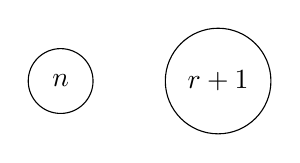
\begin{tikzpicture}
		\node[draw, circle, inner sep=2mm] at (0,0) {$n$};
		\node[draw, circle, inner sep=2mm] at (2,0) {$r+1$};
	\end{tikzpicture}
	\]
	即第一组有 \( n \) 个元素，第二组有 \( r+1 \) 个元素（记为 \( r_0, r_1, \dots, r_r \)）。
	
	现在，我们按“是否选第二组中的某个元素”来分类讨论：
	\begin{enumerate}
		\item \( \dbinom{n+r}{r} \)：不选第二组中的 \( r_0\) ，只从第一组 \( n \) 个元素和第二组的 \( r \) 个剩余元素中选 \( r \) 个。
		\item \( \dbinom{n+r-1}{r-1} \)：选第二组中的 \( r_0 \)，不选 \( r_1 \)，再从其余 \( n+r-1 \) 个元素中选 \( r-1 \) 个。
		\item \( \dbinom{n+r-2}{r-2} \)：选 \( r_0, r_1 \)，不选 \( r_2 \)，再从其余 \( n+r-2 \) 个元素中选 \( r-2 \) 个。
		\item \(\vdots\)
		\item \( \dbinom{n+1}{1} \)：选 \( r_0, r_1, \dots, r_{r-2} \)，不选 \( r_{r-1} \)，再从其余 \( n+1 \) 个元素中选 \( 1 \) 个。
		\item \( \dbinom{n}{0} \)：选 \( r_0, r_1, \dots, r_{r-1} \)，不选 \( r_r \)，从其余 \( n \) 个元素中选 \( 0 \) 个。
	\end{enumerate}
	
	所有情况相加，恰好覆盖了从 \( n+r+1 \) 个元素中选 \( r \) 个的全部可能，故等式成立。
\end{proof}


\begin{theorem}
	若 \( m,n \in \mathbb{N} \)，则 \[ \sum_{k=0}^{m}\binom{m}{k}\binom{n}{k} = \binom{m+n}{m} \]
\end{theorem}

\begin{proof}
	由组合数性质 \( \binom{m}{k} = \binom{m}{m-k} \)，将原式变形为：
	\[
	\sum_{k=0}^{m}\binom{m}{k}\binom{n}{k} = \sum_{k=0}^{m}\binom{m}{m-k}\binom{n}{k}
	\]
	上式可解释为：从两个不相交集合 \( A = \{a_1,a_2,\dots,a_m\} \) 和 \( B = \{b_1,b_2,\dots,b_n\} \) 中选取 \( m \) 个元素的组合数（其中从 \( A \) 选 \( m-k \) 个，从 \( B \) 选 \( k \) 个）。根据组合数的定义，其结果为 \( \binom{m+n}{m} \)。
	
	更一般地，\[\sum_{k=0}^{r}\binom{m}{r-k}\binom{n}{k}=\binom{m+n}{r}\]上面那个式子有的时候被称作 Vandermonde 公式
\end{proof}

\begin{theorem}
	\( \sum_{k=0}^{n}\binom{n}{k}^2 = \binom{2n}{n} \)
\end{theorem}

\begin{proof}
	令 \( m = n \)，代入上一定理的结论，可得：
	\[
	\sum_{k=0}^{n}\binom{n}{k}\binom{n}{k} = \sum_{k=0}^{n}\binom{n}{k}^2 = \binom{n+n}{n} = \binom{2n}{n}
	\]
\end{proof}

\begin{theorem}
	\( \sum_{i=0}^{n}\binom{i}{k} = \binom{n+1}{k+1} \)（\( k \leq n \)）
\end{theorem}

\begin{proof}
	把左面展开，右面相当于是从 \(n+1\) 个里取出 \(k+1 \) 个，现在看左面，\(\binom{n}{k}\) 这一项是选了 \(a_0\) 之后，从剩下的 \(n\) 个里面选，第二项是没选 \(a_0\) 但是选择了 \(a_1\) 的方法数，以此类推得到左面的式子。
\end{proof}

\begin{theorem}
	\( \binom{n}{l}\binom{l}{r} = \binom{n}{r}\binom{n-r}{l-r} \)（\( r \leq l \leq n \)）
\end{theorem}

\begin{proof}
	暴力展开。
\end{proof}


\section{线排列、圆排列、重集上的排列}
\subsection{线排列和圆排列}
线排列是普通意义上的排列，圆排列仅需除元素个数，较易，跳过。
\subsection{重集上的排列}
\begin{definition}
	称由 \( k_1 \) 个 \( b_1 \)，\( k_2 \) 个 \( b_2 \)，\(\dots\)，\( k_n \) 个 \( b_n \) 构成的集合  
	\[B = \{k_1 * b_1, k_2 * b_2, \cdots, k_n * b_n\}\]为重集，其中：\( b_i \) 为 \( n \) 个互不相同的元素，称 \( k_i \) 为 \( b_i \) 的重数，\( i = 1, 2, \cdots, n \)，\( n = 1, 2, \cdots, \infty \)，\( k_i = 1, 2, \cdots, \infty \)。
\end{definition}
\begin{definition}[集合论定义]
	从 \( n \) 个不同元素中，可重复选取 \(r\)个按一定顺序排列起来，称为重排列。
	
	从重集 \( B=\{k_1 * b_1, k_2 * b_2, \ldots, k_n * b_n\} \) 中选取一个按一定顺序排列起来。
\end{definition}

\begin{theorem}
	重集 \( B=\{\infty * b_1, \infty * b_2, \ldots, \infty * b_n\} \) 的 \(r\) 排列的个数为 \( n^r \)。
\end{theorem}

\begin{proof}
	构造 \( B \) 的 \(r\) 排列如下：选择第一项时可以从 \( n \) 个元素中任选一个，有 \( n \) 种选法，选择第二项时由于可以重复选取，仍有 \( n \) 种选法\(\dots\)，同理，选择第 \( r \) 项时仍有 \( n \) 种选法，根据乘法法则，可得出 \( r \) 排列的个数为 \( n^r \)。
\end{proof}
\begin{definition}
	重集 $B=\{n_1*b_1, n_2*b_2, \ldots, n_k*b_k\}$ 的全排列个数为  
	\[\frac{n!}{n_1! \times n_2! \times \cdots \times n_k!},\]
	其中 $n = \sum_{i=1}^k n_i$。
\end{definition}

\begin{proof}
	将 $B$ 中的 $n$ 个 $b_i$ 看作不同的 $n$ 个元素，赋予上标 $1, 2, \ldots, n_i$，即 $b_i^1, b_i^2, \ldots, b_i^{n_i} (i=1, 2, \ldots, k)$，如此，重集 $B$ 就变成具有 $n_1+n_2+\cdots+n_k=n$ 个不同的元素集合
	\[A=\{b_1^1, b_1^2, \ldots, b_1^{n_1}, b_2^1, \ldots, b_2^{n_2}, \ldots b_{k}^1, \ldots, b_{k}^{n_k}\}\]
	显然，集合 $A$ 的全排列个数为 $n!$。
	
	又由于 $n_i$ 个 $b_i$ 赋予上标的方法有 $n_i!$ 种，于是对重集 $B$ 的任一个全排列，都可以产生集合 $A$ 的 $n_1!\times n_2!\times \cdots \times n_k!$ 个排列（由乘法法则），故重集 $B$ 的全排列个数为
	\[\frac{n!}{n_1! \times n_2! \times \cdots \times n_k!},\]
	其中 $n = \sum_{i=1}^k n_i$。
\end{proof}
\begin{remark}
利用组合数的计数方法同样可以得出证明。
\end{remark}

\begin{example}
	有四面红旗，三面蓝旗，二面黄旗，五面绿旗可以组成多少种由14面旗子组成的一排彩旗？
\end{example}
\begin{sol}
求重集 $\{4*\text{红旗}, 3*\text{蓝旗}, 2*\text{黄旗}, 5*\text{绿旗}\}$ 的全排列个数，根据定理，一排彩旗的种数为
	\[ \frac{14!}{4!\times 3!\times 2!\times 5!} = 2522520 \]
\end{sol}

\begin{example}
	用字母A、B、C组成五个字母的符号，要求A至多出现2次，B至多出现1次，C至多出现3次。求此类符号的个数。
\end{example}
\begin{sol}
	设字母A、B、C的出现次数分别为 \(a\)、\(b\)、\(c\)，则满足：
	\[
	a + b + c = 5, \quad 0 \leq a \leq 2, \quad 0 \leq b \leq 1, \quad 0 \leq c \leq 3.
	\]
	列出所有满足条件的 \((a, b, c)\) 组合 \((2, 0, 3)\),\((1, 1, 3)\),\((2, 1, 2)\)相当于去考虑这三个重集的排列。
	
	对于每个组合，计算排列数（多重集排列）：\\
	对于 \((2, 0, 3)\)：\(\frac{5!}{2! \cdot 0! \cdot 3!} = \frac{120}{2 \cdot 1 \cdot 6} = 10\)\\
	对于 \((1, 1, 3)\)：\(\frac{5!}{1! \cdot 1! \cdot 3!} = \frac{120}{1 \cdot 1 \cdot 6} = 20\)\\
	对于 \((2, 1, 2)\)：\(\frac{5!}{2! \cdot 1! \cdot 2!} = \frac{120}{2 \cdot 1 \cdot 2} = 30\)\\
	总符号个数为：
	\[
	10 + 20 + 30 = 60
	\]
	因此，此类符号的个数为 60。
\end{sol}




\section{无重组合、重复组合、不相邻的组合}
\subsection{无重组合}
大家应该都知道这是什么，所以我不写了（。
\subsection{重复组合}
\begin{theorem}
	从 \( n \) 个不同元素中可重复选取 \( r \) 个的组合数，（也就是\( A=\{\infty * a_1, \infty * a_2, \ldots, \infty * a_n\} \)）和从 \( n+r-1 \) 个不同元素中不重复选取 \( r \) 个的组合数是相同的，故\[F(n,r) = C(n+r-1, r)\]
\end{theorem}
这是一个经典的组合恒等式，在组合数学中有着重要应用。公式中的 $F(n,r)$ 表示可重复组合数，$C(n+r-1, r)$ 表示普通的组合数（二项式系数）。
\begin{proof}
	设 \( n \) 个元素 \( b_1, b_2, \ldots, b_n \) 和自然数 \( 1, 2, \ldots, n \) 一一对应。于是任何组合皆可看作是一个 \( r \) 个数的组合 \(\{c_1, c_2, \ldots, c_r\}\)。由于是组合，不妨认为各 \( c_i \) 是按照大小顺序排列的，相同的 \( c_i \) 连续排在一起，不妨设 \( c_1 \leq c_2 \leq \ldots \leq c_r \)。
	
	又令 \( d_i = c_i + i - 1 \ (i = 1, 2, \ldots, r) \)，即 \( d_1 = c_1, d_2 = c_2 + 1, \ldots, d_r = c_r + r - 1 \)。
	
	因 \( 1 \leq c_i \leq n \)，故 \( 1 \leq d_i \leq n + r - 1 \)，得到一个集合 \(\{1, 2, \ldots, n + r - 1\}\) 的 \(r\) 组合 \(\{d_1, d_2, \ldots, d_r\} \ (d_1 < d_2 < \ldots < d_r)\)。
	
	显然有一种 \(\{c_1, c_2, \ldots, c_r\}\) 的取法，就有一种 \(\{d_1, d_2, \ldots, d_r\}\) 的取法，反之亦然，这两种取法是一一对应的，从而这两种取法是等价的。如此，从 \( n \) 个不同元素中可重复选取 \( r \) 个的组合数，和从 \( n + r - 1 \) 个不同元素中不重复选取 \( r \) 个的组合数是相同的，故
	
	\[F(n, r) = C(n + r - 1, r)\]
\end{proof}
\begin{theorem}
	$r$ 个无区别的球放入 $n$ 个有标志的盒子里，每盒的球数可多于 $1$ 个，则共有 $F(n,r)$ 种方案。
\end{theorem}

\begin{proof}
	这是一个允许重复组合的典型问题，实质上定理 2.6 的另一种说法。由于每盒的球数不受限制，相当于重集 $\{ \infty^* a_1, \infty^* a_2, \ldots, \infty^* a_n \}$ 的一组合。
\end{proof}

\begin{example}
试问 $(x+y+z)^4$ 的展开式有多少项？
\end{example}
\begin{sol}
	 $(x+y+z)^4$ 展开式每一项都是 $4$ 次方的，相当于从 $3$ 个不同元素中可以重复的选择 $4$ 个，或者相当于将 $4$ 个无区别的球放到 $3$ 个有标志的盒子里。故展开项个数为  
	\[F(3,4)=C(3+4-1,4)=15\]
\end{sol}
\begin{example}
	求 \( n \) 个无区别的球放入 \( r \) 个有标志的盒子里 (\( n \geq r \)) 而无一空盒的方案数。
\end{example}
\begin{sol}
由于每个盒子不能为空，故每个盒子里可先放一个球，这样还剩 \( n-r \) 个球，再将这 \( n-r \) 个球放到 \( r \) 个盒子里，由于这时每盒的球数不受限制，相当于重集 \(\{ \infty^*a_1, \infty^*a_2, \ldots, \infty^*a_r \}\) 的 \( n-r \) 组合。根据定理2.6知，其组合数为
\[F(r,n-r) = C(r+n-r-1,n-r) = C(n-1,r-1)\]
\end{sol}
\begin{example}
	某餐厅有7种不同的菜，为了招待朋友，一个顾客需要买14个菜，问有多少种买法？
\end{example}
\begin{sol}
	这个问题相当于重集 \(\{ \infty^*1, \infty^*2, \ldots, \infty^*7 \}\) 的14-组合。根据定理2.6知买菜的方法数为
\[F(7,14) = C(7+14-1,14) = 4845\]
\end{sol}
\begin{example}
	求方程 \( x_1 + x_2 + \ldots + x_n = r \) 的非负整数解的个数，其中 \( n, r \) 为正整数。
\end{example}
\begin{sol}
	设重集 \( B = \{ \infty * b_1, \infty * b_2, \ldots, \infty * b_n \} \)，\( B \) 的任一个 \( r \) 组合都具有形式 \(\{ x_1 * b_1, x_2 * b_2, \ldots, x_n * b_n \}\)，其中 \( x_i (i=1, 2, \ldots, n) \) 是非负整数且满足方程 \( x_1 + x_2 + \ldots + x_n = r \)。

反之，每一个满足方程 \( x_1 + x_2 + \ldots + x_n = r \) 的非负整数解 \( x_1, x_2, \ldots, x_n \) 都对应重集 \( B \) 的一个 \( r \) 组合。因此，方程 \( x_1 + x_2 + \ldots + x_n = r \) 的非负整数解的个数就等于重集 \( B \) 的一组合数 \( F(n, r) \)。
\end{sol}
\subsection{不相邻组合}
\begin{definition}
	从序列 \( A=\{1,2,\ldots,n\} \) 个中选取 \( r \) 个，其中不存在 \( i,i+1 \) 两个相邻的数同时出现于一个组合的组合。
\end{definition}

\begin{theorem}
	从序列 \( A=\{1,2,\ldots,n\} \) 中选取 \( r \) 个作不相邻的组合，其组合数为 \( C(n-r+1,r) \)
\end{theorem}
\begin{proof}
	设 \(\{d_1, d_2, \ldots, d_r\}\) 是所求的一个不相邻组合，不妨设 \(d_1 < d_2 < \cdots < d_r\)。令 \(c_i = d_i - i + 1 \ (i = 1, 2, \ldots, r)\)，即 \(c_1 = d_1, c_2 = d_2 - 1, \ldots, c_r = d_r - r + 1\)。因 \(1 \leq d_i \leq n\)，故 \(1 \leq c_i \leq n - r + 1\)，得到一个集合 \(\{1, 2, \ldots, n - r + 1\}\) 的一组合。显然有一种 \(\{d_1, d_2, \ldots, d_r\}\) 的取法，就有一种 \(\{c_1, c_2, \ldots, c_r\}\) 的取法反之亦然，集合 \(\{1, 2, \ldots, n - r + 1\}\) 的一个 \(r-\) 组合 \(\{c_1, c_2, \ldots, c_r\}\)，不妨设 \(c_1 < c_2 < \cdots < c_r\)。令 \(d_i = c_i + i - 1 \ (i = 1, 2, \ldots, r)\)，即 \(d_1 = c_1, d_2 = c_2 + 1, \ldots, d_r = c_r + r - 1\)。因 \(1 \leq c_i \leq n - r + 1\)，故 \(1 \leq d_i \leq n\)，得到一个集合 \(\{1, 2, \ldots, n\}\) 的不相邻组合 \(\{d_1, d_2, \ldots, d_r\}\)。显然有一种 \(\{c_1, c_2, \ldots, c_r\}\) 的取法，就有一种 \(\{d_1, d_2, \ldots, d_r\}\) 的取法。
	
	故这两种取法是一一对应的，从而这两种取法是等价的。从 \(n\) 个不同元素中选取 \(r\) 的不相邻组合数，和从 \(n - r + 1\) 个不同元素中选取 \(r\) 的组合数是相同的，即 \(C(n - r + 1, r)\)。
\end{proof}
在生成函数那个单元里我们会几乎全部重新考虑这些问题。

	\section{有限制排列、棋盘多项式}
	\subsection{有限制排列}
	\begin{definition}
		（错排）设 \( S = \{1, 2, \dots, n\} \)，若排列 \( \sigma: S \to S \) 满足 \( \sigma(i) \neq i \) 对所有 \( i \in S \) 成立，则称 \( \sigma \) 为 \( S \) 的一个错排。\( n \) 个元素的错排数记为 \( D_n \)。
	\end{definition}
	
	\begin{theorem}
		错排数的计算公式为：
		\[
		D_n = n! \left( 1 - \frac{1}{1!} + \frac{1}{2!} - \frac{1}{3!} + \dots + (-1)^n \frac{1}{n!} \right)
		\]
	\end{theorem}
	
	\begin{proof}
		利用容斥原理推导。设 \( S \) 为 \( n \) 个元素的所有排列构成的集合，显然 \( |S| = n! \)。
		定义事件 \( A_i \)（\( i = 1, 2, \dots, n \)）为“第 \( i \) 个元素在原位”的排列集合。
		\begin{enumerate}
			\item 计算 \( |A_i| \)：若第 \( i \) 个元素固定在原位，剩下 \( n - 1 \) 个元素可任意排列，故 \( |A_i| = (n - 1)! \)。
			\item 计算 \( |A_i \cap A_j| \)（\( i \neq j \)）：若第 \( i \)、\( j \) 个元素都固定在原位，剩下 \( n - 2 \) 个元素可任意排列，故 \( |A_i \cap A_j| = (n - 2)! \)。
			\item 推广到 \( k \) 个事件的交集：若 \( k \) 个元素都固定在原位，剩下 \( n - k \) 个元素可任意排列，故 \( |A_{i_1} \cap A_{i_2} \cap \dots \cap A_{i_k}| = (n - k)! \)。
		\end{enumerate}
		
		根据容斥原理:
		\[
		\begin{aligned}
			D_n &= |S| - \sum_{i=1}^n |A_i| + \sum_{1 \leq i < j \leq n} |A_i \cap A_j| - \dots + (-1)^n |A_1 \cap \dots \cap A_n| \\
			D_n &= n! - \binom{n}{1}(n - 1)! + \binom{n}{2}(n - 2)! - \dots + (-1)^n \binom{n}{n} 0! \\
			D_n &= n! \left( 1 - \frac{1}{1!} + \frac{1}{2!} - \frac{1}{3!} + \dots + (-1)^n \frac{1}{n!} \right)
		\end{aligned}
		\]
	\end{proof}
	
	
	\begin{theorem}
		错排数的递推关系为：
		\[
		D_n = (n - 1)(D_{n - 1} + D_{n - 2})
		\]
	\end{theorem}
	
	\begin{proof}
		考虑第 \( n \) 个元素的放置，它不能放在第 \( n \) 位，假设放在第 \( k \) 位（\( k \neq n \)）。此时分两种情况：
		\begin{enumerate}
			\item 第 \( k \) 个元素放在第 \( n \) 位。此时剩下 \( n - 2 \) 个元素需错排，错排数为 \( D_{n - 2} \)。
			\item 第 \( k \) 个元素不放在第 \( n \) 位。可将第 \( n \) 位视为“第 \( k \) 个元素的原位”，此时 \( n - 1 \) 个元素需错排，错排数为 \( D_{n - 1} \)。
		\end{enumerate}
		由于 \( k \) 有 \( n - 1 \) 种选择（\( k = 1, 2, \dots, n - 1 \)），因此递推关系为：
		\[
		D_n = (n - 1)(D_{n - 1} + D_{n - 2})
		\]
	\end{proof}
	\begin{definition}
		（有限制排列 \(Q_n\)）设 \(Q_n\) 是集合 \(S = \{1,2,3,\dots,n\}\) 的排列中，不出现\( 12,23,34,\dots (n-1)n \)这样的排列数。
	\end{definition}
	
	\begin{theorem}
		\(Q_n\) 的计算公式为：
		\[
		\begin{aligned}
			Q_n &= n! - \binom{n-1}{1}(n-1)! + \binom{n-1}{2}(n-2)! + \dots + (-1)^{n-1}\binom{n-1}{n-1}1! \\
			&= n! + \sum_{i=0}^{n-2} (-1)^{i-1} \binom{n-1}{i+1} (n-i-1)!
		\end{aligned}
		\]
	\end{theorem}
	
	\begin{proof}
		设 \(A_i\) 是出现“ \( (i-1)i\)”这种形式的排列的集合（\(i = 1,2,\dots,n\)）。
		\begin{enumerate}
			\item 单个集合：\(|A_i| = (n-1)!\).
			\item 两个集合的交集 \(A_i \cap A_j\) 有以下两种情况：\\
			(i) 若 \(i = j-1\)，则将 \(i, i+1\) 视为一个“块”，剩余 \(n-2\) 个元素（含此块）任意排列，故 \(|A_i \cap A_j| = (n-2)!\)。\\
			(ii) 若 \(i < j-1\)，同理，固定 \(i\) 在第 \(i\) 位、\(j\) 在第 \(j\) 位后，剩余 \(n-2\) 个元素任意排列，故 \(|A_i \cap A_j| = (n-2)!\)。
			故两个集合的交计算出的结果一定是\((n-2)!\)。
			\item 相类似的进行分析，一般地，\(k\) 个这样的集合交集的大小为 \((n-k)!\)。
		\end{enumerate}
		
		根据容斥原理， \(Q_n\) 是所有“非 \(A_i\)”集合的交集的大小，即：
		\[
		\begin{aligned}
			Q_n &= \left| \overline{A_1} \cap \overline{A_2} \cap \dots \cap \overline{A_n} \right| \\
			&= |S| - \sum|A_i| + \sum|A_i \cap A_j| - \dots + (-1)^n \sum|A_1 \cap A_2 \cap \dots \cap A_n| \\
			&= n! - \binom{n-1}{1}(n-1)! + \binom{n-1}{2}(n-2)! - \dots + (-1)^{n-1}\binom{n-1}{n-1}1!
		\end{aligned}
		\]
	\end{proof}
	
	实际上 \(Q_n\) 和 \(D_n\) 在展开式上的差距仅仅在于组合数，一个是从 \( n \) 中进行选择，另一个是 \(n-1\) 。所以存在另一个递推：
	\begin{theorem}
		\(Q_n=D_n+D_{n-1}\)。
	\end{theorem}
	
	\begin{proof}
		懒得写了，反正很简单。
	\end{proof}
	
	
	\subsection{禁区排列问题及棋盘多项式递推证明}
	接下来描述一个具体的问题，这被称为禁区排列问题。且在本节将利用所谓的棋盘多项式去解决（此处不理解可先阅读生成函数一节）

	布子规定：无对攻，每行/列仅有一个子，保证 \( n \times n \) 棋盘可下 \( n \) 个子，研究 \( k \) 个子分布在棋型 \( C \) 上的方案数相关问题。
	
	为了便于叙述，我们用 \( C_i \)来指代棋盘格的图案：
	
	\begin{center}
		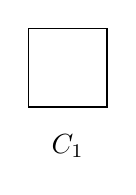
\begin{tikzpicture}
			\draw (0,0) rectangle (1,1); % 绘制1x1矩形，即“口”
			\node at (0.5,-0.5) {$C_1$};
		\end{tikzpicture}\quad\quad
		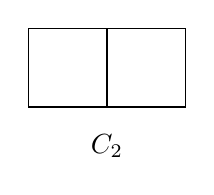
\begin{tikzpicture}
			\draw (0,0) rectangle (1,1); 
			\draw (1,0) rectangle (2,1); % 并排绘制两个1x1矩形，组成“日”型（横向）
			\node at (1,-0.5) {$C_2$};
		\end{tikzpicture}\quad\quad
		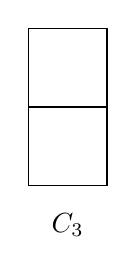
\begin{tikzpicture}
			\draw (0,0) rectangle (1,1); 
			\draw (0,1) rectangle (1,2); % 纵向堆叠两个1x1矩形
			\node at (0.5,-0.5) {$C_3$};
		\end{tikzpicture}
	\end{center}
	
	\begin{definition}
		\( \mathscr{R}_i(C_i)  \) ：使用了i个棋子放在图 $C_i$ 中的方法数。
	\end{definition}
	比如说 \( \mathscr{R}_1(C_1) =1\) ，\( \mathscr{R}_1(C_2) =2\) 等等。但是如果无论如何都摆不下的话，结果就是0.
	
	\begin{definition}
		\( C \) 可推广为任意棋型。定义下面的两种“对于棋型中某一格”的操作（但是在表达式中，我们不去指明操作的对象）：\\
		\( C_{(i)} \)：对棋型 \( C \) 进行“去除这一行和这一列”的操作后剩余的棋型；\\
		\( C_{(e)} \)：对棋型 \( C \) 进行“只去掉这一格”的操作后剩余的棋型：\\
		此时可以推出：
		\[
		\mathscr{R}_k(C) = \mathscr{R}_{k - 1}(C_{(i)}) + \mathscr{R}_k(C_{(e)})
		\]
		这一递推关系将在下图中得到简要的说明。
	\end{definition}
	
	\begin{center}
		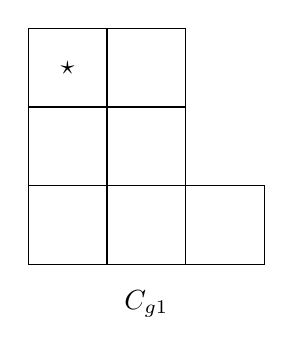
\begin{tikzpicture}
			% 第一列三个方格
			\draw (0,2) rectangle (1,3); 
			\node at (0.5, 2.5) {$\star$};
			\draw (0,1) rectangle (1,2); 
			\draw (0,0) rectangle (1,1); 
			% 第二列两个方格
			\draw (1,1) rectangle (2,3);
			\draw (1,1) rectangle (2,2); 
			\draw (1,0) rectangle (2,1); 
			% 第三列一个方格
			\draw (2,0) rectangle (3,1); 
			\node at (1.5,-0.5) {$C_{g1}$};
		\end{tikzpicture}
		\begin{tikzpicture}
			% 第一列三个方格
			
			% 第二列两个方格
			\draw (1,1) rectangle (2,2); 
			\draw (1,0) rectangle (2,1); 
			% 第三列一个方格
			\draw (2,0) rectangle (3,1); 
			\node at (1.5,-0.5) { $C_{g2}$：针对标记格的 \( C_{(i)} \) 图};
		\end{tikzpicture}
		\begin{tikzpicture}
		% 第一列
		\draw (0,1) rectangle (1,2); 
		\draw (0,0) rectangle (1,1); 
		% 第二列两个方格
		\draw (1,1) rectangle (2,3);
		\draw (1,1) rectangle (2,2); 
		\draw (1,0) rectangle (2,1); 
		% 第三列一个方格
		\draw (2,0) rectangle (3,1); 
		\node at (1.5,-0.5) { $C_{g3}$：针对标记格的 \( C_{(e)} \) 图};
		\end{tikzpicture}
	\end{center}
	
	不难想象，如果加星号的格子已经填入了一枚棋子，那它所在行和列的格子自然就无法再次填入棋子，也就是说，使用剩下的 \( k-1 \) 个棋子去填入被标记格的 的 \( C_{(i)} \) 图；如果没填入这一枚棋子，那仍然剩下了 \( k \) 个棋子去填入所谓的 \( C_{(2)} \) 图。递推关系自然得到了说明。
	
	一般情况下的证明在此略掉。
	\begin{definition}
		定义多项式 \( R(C) \) 为：
		\[
		R(C) = \sum_{k = 0}^n \mathscr{R}_k(C) x^k
		\]
		其中 \( n \) 为棋型 \( C \) 最多可布子数。
			\end{definition}
		\begin{theorem}
			\(R(C) = xR(C_{(i)}) + R(C_{(e)}).\)
		\end{theorem}
		\begin{proof}
			\[
			\begin{aligned}
				R(C) =\sum_{k = 0}^n \mathscr{R}_k(C) x^k &= 1+\sum_{k = 1}^{n} \mathscr{R}_{k - 1}(C_{(i)}) x^k + \sum_{k = 1}^n \mathscr{R}_k(C_{(e)}) x^k \\
				&= \sum_{k = 1}^{n} \mathscr{R}_{k - 1}(C_{(i)}) x^k + \sum_{k = 0}^n \mathscr{R}_k(C_{(e)}) x^k \\
				&= \sum_{k = 1}^{n} \mathscr{R}_{k - 1}(C_{(i)}) x^k +R(C_{(e)}).
			\end{aligned}
			\]
			这样接下来只需要证明
			\[
			\sum_{k = 1}^{n} \mathscr{R}_{k - 1}(C_{(i)}) x^k=xR(C_{(i)})
			\]
			就可以了。
			\[
			\begin{aligned}
				\sum_{k = 1}^{n} \mathscr{R}_{k - 1}(C_{(i)}) x^k &= \sum_{k = 0}^{n-1} \mathscr{R}_{k}(C_{(i)}) x^{k+1}\\
				&= x\sum_{k = 0}^{n-1} \mathscr{R}_{k}(C_{(i)}) x^{k}\\
				&=x\sum_{k = 0}^{n} \mathscr{R}_{k}(C_{(i)}) x^{k}\\
				&=xR(C_{(i)}).
			\end{aligned}
			\]
			其中倒数第二步成立是因为：
			\[
			\mathscr{R}_{n}(C_{(i)})
			\]
			已经没有任何办法进行棋子的填入了，删掉了一行一列之后的棋盘一定无法摆下原有的最大值，也就是 \( n \) 个棋子，由最开始对于这一记号的定义，它的结果只能是0.
			
			这样就证明了这一性质。
		\end{proof}
		
	\begin{remark}
		我们称图 \( C \) 可以被分拆成两个独立的图 \( C_1 \) 以及 \( C_2 \) 。当且仅当它们其中一个图中的任何一个格子都不在另外一个图的任意一个格子所在的行或者列。
	\end{remark}
	
	这样，有：
	\begin{theorem}
		\[
		\mathscr{R}_k(C)=\sum_{i=0}^k\left[\mathscr{R}_i(C_1)\mathscr{R}_{k-i}(C_2)\right].
		\]
	\end{theorem}
	\begin{proof}
		结论比较显然，只需要说明两部分独立就可以。
	\end{proof}
	\subsection{禁区排列}
	随后我们考虑在这个问题里面引入禁区，也就是不能摆放棋子的位置。并且把这样的排列问题叫做禁位排列。
	\begin{theorem}
		禁位排列的计数公式为：
		\[
		n! - r_1 (n-1)! + r_2 (n-2)! - \dots + (-1)^n r_n 0!
		\]
		其中，\( r_i \) 表示“有 \( i \) 个元素处于禁位”的方案数。
	\end{theorem}
	
	用容斥原理应该证的出来，但是今天累了就先鸽在这里。
	
	\begin{remark}
		一个比较有用的例子。\\
		现有 G、L、W、Y 四位工作人员，以及 A、B、C、D 四项任务，其中工作人员与任务的禁区限制如下：
		\begin{itemize}
			\item 工作人员 G 不能从事任务 B；
			\item 工作人员 L 不能从事任务 B、C 两项；
			\item 工作人员 W 不能从事任务 C、D 两项；
			\item 工作人员 Y 不能从事任务 D。
		\end{itemize}
		若要求每位工作人员各自从事一项力所能及的任务（即不违反禁区限制），且每项任务仅由一人完成，试问共有多少种不同的分配方案？
	\end{remark}
	
	可以很容易地表示成：
\begin{center}
	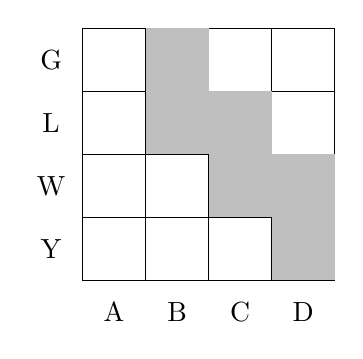
\begin{tikzpicture}[scale=0.8]
		% 绘制表格主体（4行4列）
		\draw (1,0) rectangle (5,4);  % 表格外框
		% 绘制横线
		\draw (1,1) -- (5,1);
		\draw (1,2) -- (5,2);
		\draw (1,3) -- (5,3);
		% 绘制竖线
		\draw (2,0) -- (2,4);
		\draw (3,0) -- (3,4);
		\draw (4,0) -- (4,4);
		
		% 填充阴影（禁区）
		\fill[gray!50] (2,3) rectangle (3,4); % G - B
		\fill[gray!50] (2,2) rectangle (3,3); % L - B
		\fill[gray!50] (3,2) rectangle (4,3); % L - C
		\fill[gray!50] (3,1) rectangle (4,2); % W - C
		\fill[gray!50] (4,1) rectangle (5,2); % W - D
		\fill[gray!50] (4,0) rectangle (5,1); % Y - D
		
		% 左侧标注工作人员（表格外）
		\node at (0.5, 3.5) {G};
		\node at (0.5, 2.5) {L};
		\node at (0.5, 1.5) {W};
		\node at (0.5, 0.5) {Y};
		
		% 下方标注任务
		\node at (1.5, -0.5) {A};
		\node at (2.5, -0.5) {B};
		\node at (3.5, -0.5) {C};
		\node at (4.5, -0.5) {D};
	\end{tikzpicture}
\end{center}
之后是显然的，我们把阴影记成一个图 \( C \) ，这样我们直接对这个图去求前文提到的 \( R \) 多项式，结果是：
\[
R(C)=1+6x+10x^2+4x^3.
\]
带回去就知道答案是：
\[
4!-6\times 3!+10\times 2! -4=4.
\]

然后是一些例题：
\[
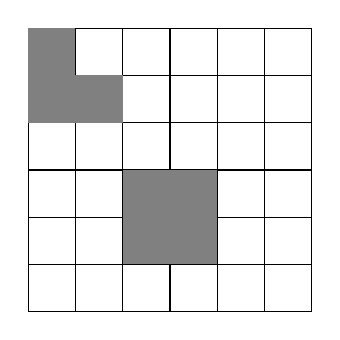
\begin{tikzpicture}[scale=0.6]
	% 绘制 6×6 网格边框
	\foreach \x in {0,...,6} \draw (\x,0) -- (\x,6);
	\foreach \y in {0,...,6} \draw (0,\y) -- (6,\y);
	
	% 填充灰色禁区
	\fill[gray] (0,5) rectangle (1,6);  % 第1行第1列（坐标从0开始，对应网格左上角）
	\fill[gray] (0,4) rectangle (2,5);  % 第2行第1-2列
	\fill[gray] (2,2) rectangle (4,3);  % 第4-5行第3-4列
	\fill[gray] (2,1) rectangle (4,2); 
\end{tikzpicture}
\]
这个的结果应该是\[
R(C)=2x^4+10x^3+15x^2+7x+1.\]
这结果应该是184.

\[
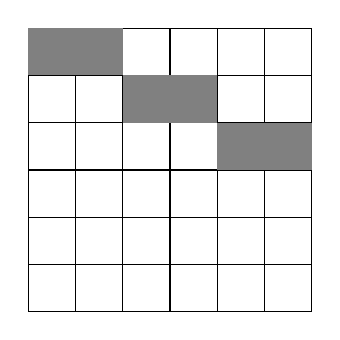
\begin{tikzpicture}[scale=0.6]
	% 绘制 6×6 网格边框
	\foreach \x in {0,...,6} \draw (\x,0) -- (\x,6);
	\foreach \y in {0,...,6} \draw (0,\y) -- (6,\y);
	
	% 填充灰色禁区
	\fill[gray] (0,5) rectangle (2,6);  % 第1行第1-2列 
	\fill[gray] (2,4) rectangle (4,5);  % 第2行第3-4列 
	\fill[gray] (4,3) rectangle (6,4);  % 第3行第5-6列 
\end{tikzpicture}\quad\quad
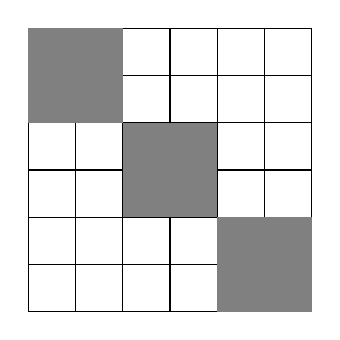
\begin{tikzpicture}[scale=0.6]
	% 绘制 6×6 网格边框
	\foreach \x in {0,...,6} \draw (\x,0) -- (\x,6);
	\foreach \y in {0,...,6} \draw (0,\y) -- (6,\y);
	
	% 填充灰色禁区
	% 左上 2×2 块（行5-6，列0-1 ，坐标从0开始，y越大越靠上）
	\fill[gray] (0,5) rectangle (2,6); 
	\fill[gray] (0,4) rectangle (2,5); 
	% 中间 2×2 块（行3-4，列2-3 ）
	\fill[gray] (2,3) rectangle (4,4); 
	\fill[gray] (2,2) rectangle (4,3); 
	% 右下 2×2 块（行1-2，列4-5 ）
	\fill[gray] (4,1) rectangle (6,2); 
	\fill[gray] (4,0) rectangle (6,1); 
\end{tikzpicture}\]
这俩我没算，以后再说。

还有个更复杂的：
\[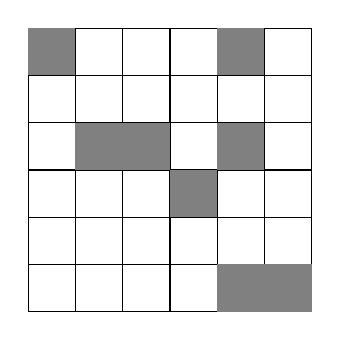
\begin{tikzpicture}[scale=0.6]
	% 绘制 6×6 网格边框
	\foreach \x in {0,...,6} \draw (\x,0) -- (\x,6);
	\foreach \y in {0,...,6} \draw (0,\y) -- (6,\y);
	
	% 填充灰色禁区，坐标 (x列起始, y行起始) 到 (x列结束, y行结束)，y越大越靠上
	\fill[gray] (0,5) rectangle (1,6);   % 第1行第1列
	\fill[gray] (4,5) rectangle (5,6);   % 第1行第5列
	\fill[gray] (1,3) rectangle (3,4);   % 第3行第2-3列
	\fill[gray] (4,3) rectangle (5,4);   % 第3行第5列
	\fill[gray] (3,2) rectangle (4,3);   % 第4行第4列
	\fill[gray] (4,0) rectangle (6,1);   % 第6行第5-6列
\end{tikzpicture}\]
交给复习的自己。
\subsection{$Introductory\ Combinatorics$的一道例题——正解}
\begin{proposition}
	（本例摘自 $ Richard\ A.\ Brualdi$ 的 $Introductory\ Combinatorics$ 中第六单元33小题，原题目疑似有误，下面是原题）
	设 \( n \) 和 \( k \) 是正整数且 \( k \leq n \)。设 \( a(n, k) \) 是把 \( k \) 个非攻击型车放到 \( n \times n \) 棋盘上的摆放方法数，其中棋盘上的位置 \( (1, 1) \)，\( (2, 2) \)，\( \dots \)，\( (n, n) \) 和 \( (1, 2) \)，\( (2, 3) \)，\( \dots \)，\( (n-1, n) \)，\( (n, 1) \) 是禁止位置。\\
	证明：\\
	 \[ a(n, k) =\frac{2n}{2n-k}\binom{2n-k}{k}.\]
	 \begin{textblock*}{\textwidth}(0pt, \dimexpr\paperheight - 2cm\relax)
	 	\centering  % 新增居中命令，让里面的横线和文字居中
	 	\hrule width \textwidth height 0.4pt 
	 	\vspace{5pt} 
	 	\small 原书上的描述是“不在禁区之内”，应该是错的。
	 \end{textblock*}
	提示：\\
	这里的 \( a(n, k) \) 也是从 \( 2n \) 个孩子中选择 \( k \) 个孩子并且使得没有两个相邻孩子被选中的方法数。
	
	而实际上，这里的 \( a(n, k) \) 应该正是在禁区中的排列数，原书应该有误。所以正确的题目应该是：
\end{proposition}
\begin{remark}
	设 \( n \) 和 \( k \) 是正整数且 \( k \leq n \)。设 \( a(n, k) \) 是把 \( k \) 个非攻击型车放到 \( n \times n \) 棋盘上位置 \( (1, 1) \)，\( (2, 2) \)，\( \dots \)，\( (n, n) \) 和 \( (1, 2) \)，\( (2, 3) \)，\( \dots \)，\( (n-1, n) \)，\( (n, 1) \) 的方法数。
\end{remark}
下面是一张 \( n=6\) 的示例图。


\[	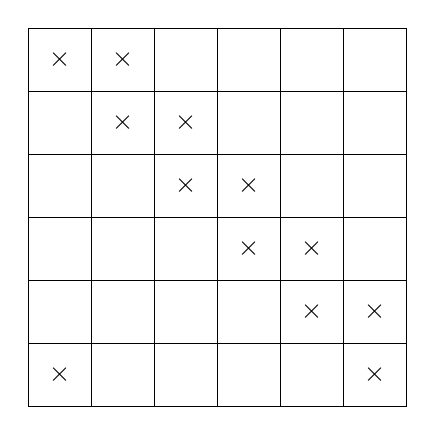
\begin{tikzpicture}[scale=0.8]
	% 绘制6×6棋盘
	\foreach \x in {0,1,2,3,4,5}
	\foreach \y in {0,1,2,3,4,5}
	\draw (\x,\y) rectangle (\x+1,\y+1);
	
	% 原始图形顺时针旋转90度后，各×的位置计算：
	% 原坐标(x,y)旋转后变为(y, 5-x)（因为是0-5的坐标范围）
	
	% 1. 主对角线的×（原位置(0,0),(1,1),...,(5,5)）
	% 旋转后应为(0,5),(1,4),(2,3),(3,2),(4,1),(5,0)
	\node at (0+0.5,5+0.5) {$\times$};  % 原(0,0)
	\node at (1+0.5,4+0.5) {$\times$};  % 原(1,1)
	\node at (2+0.5,3+0.5) {$\times$};  % 原(2,2)
	\node at (3+0.5,2+0.5) {$\times$};  % 原(3,3)
	\node at (4+0.5,1+0.5) {$\times$};  % 原(4,4)
	\node at (5+0.5,0+0.5) {$\times$};  % 原(5,5) - 这是旋转后的左下角，保留
	
	% 2. 右上对角线的×（原位置(0,1),(1,2),...,(4,5)）
	% 旋转后应为(1,5),(2,4),(3,3),(4,2),(5,1)
	\node at (1+0.5,5+0.5) {$\times$};  % 原(0,1) - 这是旋转后的左上角，需要移动
	\node at (2+0.5,4+0.5) {$\times$};  % 原(1,2)
	\node at (3+0.5,3+0.5) {$\times$};  % 原(2,3)
	\node at (4+0.5,2+0.5) {$\times$};  % 原(3,4)
	\node at (5+0.5,1+0.5) {$\times$};  % 原(4,5)
	
	% 3. 原(5,0)位置的×
	% 旋转后应为(0,0)
	% 注释掉原来的左上角×，改为放到左下角
	% \node at (0+0.5,0+0.5) {$\times$};  % 原(5,0) - 旋转后左上角，不使用
	
	% 将旋转后左上角的×（原(0,1)）放到左下角
	\node at (0+0.5,0+0.5) {$\times$};
\end{tikzpicture}\]

先证引理：
\begin{lemma}
	这里的 \( a(n, k) \) 也是从 \( 2n \) 个孩子中选择 \( k \) 个孩子并且使得没有两个相邻孩子被选中的方法数。
\end{lemma}
\begin{proof}
	对于每一个孩子，不能选择相邻的孩子，那么我们任意的取一个点，它的相邻的点不能被选择，于是被划分到另外一集中，如此划分可以把这个2n的环恰好划分成两个集合，把不能够同时取的两个元素之间连线其他不连，就构成了一张成环的二分图。
	
	建模完毕，然后来求解，首先关注一个线性的队列，不让两两孩子相邻被选中的方法应该进行插空。方法数是：
	\[\binom{n-k+1}{k}\]
	这样的话，那个环形的方法数就要破环：
	第一个如果没有被选，就是长度为 \(2n-1 \) 的链取 \(k\) ，选了的话，第二个和最后一个都不能被选中，就是从长度为 \( 2n-3 \) 的链里面选择 \(k-1\) 个，这结果总共就应该是：
	\[\binom{2n-1-k+1}{k}+\binom{2n-3-(k-1)+1}{k-1}=\frac{2n}{2n-k}\binom{2n-k}{k}.\]
\end{proof}
然后我们来说明为什么在这种禁区里面摆放棋子和这个环是等价的。
\begin{proof}
	考虑随便的一个 \((i,i)\) 这样它一共会影响到两个点，一个是 \((i,i+1 )\) ，另一个是 \((i+1,i)\)（超过 \(n\) 了就取模）。这样也同刚才的引理，我们通过选择了一个点来限制住了另外的两个点，且可以通过这样的方式去把它连成一个环，和引理一样。那结论自然完全一样。
\end{proof}
\subsection{其他推出的内容及结论}
然后看一下为了做这个题的一些努力（失败的尝试）：

探讨在以下的图中应该如何去摆放车：
\[\begin{tikzpicture}[scale=0.8]
	% 第一列
	\draw (0,2) rectangle (1,3); 
	\draw (0,1) rectangle (1,2); 
	% 第二列两个方格
	\draw (1,1) rectangle (2,2); 
	\draw (1,0) rectangle (2,1); 
	
\end{tikzpicture}\quad\quad\quad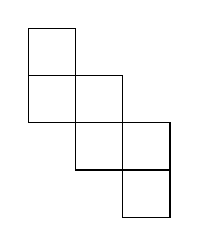
\begin{tikzpicture}[scale=0.6]
% 第一列
\draw (0,3) rectangle (1,4); 
\draw (0,2) rectangle (1,3); 
% 第二列两个方格
\draw (1,2) rectangle (2,3); 
\draw (1,1) rectangle (2,2); 
\draw (2,1) rectangle (3,2); 
\draw (2,0) rectangle (3,1); 
\end{tikzpicture}\]
这张图中有两个并排的“日”字，为了寻求其中可能有的某一种规律性，不妨将其记成 \( G_2\) 用来代表它是由两个“日”叠起来的。
这样类似的， \( G_0 \) 是 \( \varnothing\) ，\(G_3\) 是看起来像是上面靠右的图。
并且为了讨论问题方便，记
\[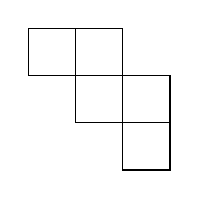
\begin{tikzpicture}[scale=0.6]
	% 第一列

	\draw (0,2) rectangle (1,3); 
	% 第二列两个方格
	\draw (1,2) rectangle (2,3); 
	\draw (1,1) rectangle (2,2); 
	\draw (2,1) rectangle (3,2); 
	\draw (2,0) rectangle (3,1); 
\end{tikzpicture}\]
是所谓的 \( G_2^*\) 。这么记的原因是它比正常的 \( G_2 \) 要多了一个方格。
利用前面我们所得到的几个定理，我们知道只要我们能求出上面那张棋盘的棋盘多项式就做得出来这个问题。而为了求解出这一多项式，我们运用前面得到过的所有定理，得到：
\[
\begin{aligned}
	& R(G_n) = x R(G_{n-2}^*) + (x+1) R(G_{n-1}) \text{（选中最左边那一列的第二个方格。然后自然得出）} \\
	& R(G_n^*) = (x+1) R(G_{n-1}^*) + x R(G_{n-1}) \text{（选中第一行的第二个方格。然后自然得出）}\\
	& x R(G_n) - (x+1) R(G_n^*) = x^2 R(G_{n-2}^*) - (x+1)^2 R(G_{n-1}^*) \\
	&  R(G_n) = \frac{x+1}{x} R(G_n^*) + x R(G_{n-2}^*) - \frac{(x+1)^2}{x} R(G_{n-1}^*) \\
	& \frac{x+1}{x} R(G_n^*) + x R(G_{n-2}^*) - \frac{(x+1)^2}{x} R(G_{n-1}^*) = x R(G_{n-2}^*) + (x+1)  R(G_{n-1})  \\
	&  = x R(G_{n-2}^*) + (x+1)\left( \frac{x+1}{x} R(G_{n-1}^*) + x R(G_{n-3}^*) - \frac{(x+1)^2}{x} R(G_{n-2}^*)\right)
\end{aligned}
\]
（注：这里式子里面出现的 \( x+1\) 是 \( R(\square)\) ）

于是推出：
\[
\begin{aligned}
	&\frac{x+1}{x} R(G_n^*)- \frac{(x+1)^2}{x} R(G_{n-1}^*) =(x+1)\left( \frac{x+1}{x} R(G_{n-1}^*) + x R(G_{n-3}^*) - \frac{(x+1)^2}{x} R(G_{n-2}^*)\right)\\
	&\frac{1}{x} R(G_n^*)- \frac{x+1}{x} R(G_{n-1}^*) =\frac{x+1}{x} R(G_{n-1}^*) + x R(G_{n-3}^*) - \frac{(x+1)^2}{x} R(G_{n-2}^*)\\
	&\text{最终：}\\
	&R(G_n^*)= 2(x+1)R(G_{n-1}^*) + x^2 R(G_{n-3}^*) - (x+1)^2R(G_{n-2}^*)
\end{aligned}
\]

然后就得到了一个递推关系式。我们使用吃奶的力气算出来前面几项：
\[
\begin{aligned}
	&G_0^*=x+1\\
	&G_1^*=x^2+3x+1\\
	&G_2^*=x^3+6x^2+5x+1.
\end{aligned}\]

然后问题立刻变成了以下的样子：

\[
\begin{pmatrix}
	G_3^* \\
	G_2^* \\
	G_1^*
\end{pmatrix}
=
\begin{pmatrix}
	2(x+1)  & - (x+1)^2 & x^2 \\
	1 & 0 & 0 \\
	0 & 1 & 0
\end{pmatrix}
\begin{pmatrix}
	G_2^* \\
	G_1^* \\
	G_0^*
\end{pmatrix}
\]
递推关系可以往下传递，变成：
\[
\begin{pmatrix}
	G_{n+2}^* \\
	G_{n+1}^* \\
	G_{n}^*
\end{pmatrix}
=
\begin{pmatrix}
	2(x+1)  & - (x+1)^2 & x^2 \\
	1 & 0 & 0 \\
	0 & 1 & 0
\end{pmatrix}^n
\begin{pmatrix}
	G_2^* \\
	G_1^* \\
	G_0^*
\end{pmatrix},\begin{pmatrix}
G_2^* \\
G_1^* \\
G_0^*
\end{pmatrix}=\begin{pmatrix}
x^3+6x^2+5x+1 \\
x^2+3x+1 \\
x+1
\end{pmatrix}
\] 
把中间的矩阵记成 \( \mathbf{X} \) ，两个列向量记成 \( \mathbf{G_n}\) （角标跟随最下面的一行）可以比较简单的写成：
\[\mathbf{G_n}=\mathbf{X}^n\mathbf{G_0}.\]
求 \( \mathbf{X} \) 的特征值：最终解得结果为：
\[\lambda_1=1\ ,\ \lambda_2=x+\frac{1+\sqrt{4x+1}}{2}\ ,\ \lambda_3=x+\frac{1-\sqrt{4x+1}}{2}\]
然后求特征向量：
分别解出来三个特征向量（记成 \( T_i ,(i=1,2,3)\) ）得：
\[
T_1=\begin{pmatrix}
	1 \\
	1 \\
	1
\end{pmatrix},\quad
T_2=\begin{pmatrix}
	\lambda_2^2 \\
	\lambda_2 \\
	1
\end{pmatrix},\quad
T_3=\begin{pmatrix}
\lambda_3^2 \\
\lambda_3 \\
1
\end{pmatrix}\] 
所以
\[\mathbf{T}=\begin{pmatrix}
	1  & \lambda_2^2 & \lambda_3^2 \\
	1 & \lambda_2 & \lambda_3 \\
	1 & 1 & 1
\end{pmatrix}\]
求这矩阵的逆：
\[\boldsymbol{T}^{-1} = \frac{1}{(\lambda_1 - \lambda_2)(\lambda_1 - \lambda_3)(\lambda_2 - \lambda_3)}
\begin{pmatrix}
	\lambda_2 - \lambda_3 & (\lambda_3 - \lambda_2)(\lambda_3 + \lambda_2) & \lambda_2\lambda_3(\lambda_2 - \lambda_3) \\
	\lambda_3 - 1 & (1 - \lambda_3)(1 + \lambda_3) & \lambda_3(\lambda_3 - 1) \\
	1 - \lambda_2 & (\lambda_2 - 1)(\lambda_2 + 1) & \lambda_2(1 - \lambda_2)
\end{pmatrix}
\]
我们知道
\[
\mathbf{X}^n=(\mathbf{T}\mathbf{\Lambda}\mathbf{T}^{-1})^n=\mathbf{T}\mathbf{\Lambda}^n\mathbf{T}^{-1}
\]

\[\mathbf{X}^n=\Delta'\begin{pmatrix}
	1  & \lambda_2^2 & \lambda_3^2 \\
	1 & \lambda_2 & \lambda_3 \\
	1 & 1 & 1
\end{pmatrix}\begin{pmatrix}
1  & 0 & 0 \\
0 & \lambda_2 & 0 \\
0 & 0 & \lambda_3
\end{pmatrix}^n\begin{pmatrix}
\lambda_2 - \lambda_3 & (\lambda_3 - \lambda_2)(\lambda_3 + \lambda_2) & \lambda_2\lambda_3(\lambda_2 - \lambda_3) \\
\lambda_3 - 1 & (1 - \lambda_3)(1 + \lambda_3) & \lambda_3(\lambda_3 - 1) \\
1 - \lambda_2 & (\lambda_2 - 1)(\lambda_2 + 1) & \lambda_2(1 - \lambda_2)
\end{pmatrix}
\]
其中 \[ \Delta'=\frac{1}{(\lambda_1 - \lambda_2)(\lambda_1 - \lambda_3)(\lambda_2 - \lambda_3)}\]

后面的表达式复杂地难以计算，理论上能得到答案但太过于困难，不赘述了。

\begin{remark}
	实际上这里的过程是可以简化的（虽然简化了也没啥用就是了）：如果特征值都不一样的话，可以直接用待定系数法来解出来，比如这里的关系式
	\[R(G_n^*)= 2(x+1)R(G_{n-1}^*) + x^2 R(G_{n-3}^*) - (x+1)^2R(G_{n-2}^*\]
	就是一个线性递推，求出来特征值之后的
	\[R(G_n^*)\]
	可以直接表成：
	\[A\lambda_1^n+B\lambda_2^n+C\lambda_3^n.\]
	将在递推关系与生成函数章节中得到证明。
\end{remark}

\chapter{**递推关系和生成函数}
\section{生成函数基础}
\subsection{普通生成函数}
\begin{example}
	掷 \( n \) 个骰子，求掷出 \( n \) 点的方法数。
	\bigskip
	
	一个例子：求解 \((x_1 + x_2 + \dots + x_6)^n\) 中 \( x^n \) 的系数。
	\[
	f(x) = (x + x^2 + \dots + x^6)^n
	\]
	即称 \( f(x) \) 为该问题的母函数。
\end{example}

\begin{definition}
	设给定无穷序列 \(\{a_0, a_1, \dots, a_k, \dots\}\)，称
	\[
	f(x) = \sum_{k=0}^{\infty} a_k x^k
	\]
	为 \(\{a_k\}\) 的普通生成函数（又成母函数）。
\end{definition}

\begin{remark}
	我们在此处并不管 \( f(x) \) 的收敛性。（其实这被称作形式幂级数）
\end{remark}

\begin{proposition}
	求序列 \(\{C(n,0), C(n,1), \dots, C(n,n)\}\) 的普通母函数。
	\[
	f(x) = \sum_{k=0}^{n} C(n,k) x^k = \binom{n}{0} + \binom{n}{1}x + \binom{n}{2}x^2 + \dots + \binom{n}{n}x^n = (1 + x)^n
	\]
\end{proposition}
\begin{remark}
	不是无穷也可以这样类似的去求解。
\end{remark}
\begin{proposition}
	求序列 \(\left\{ \binom{n-1}{0}, -\binom{n}{1}, \binom{n+1}{2}, \dots, (-1)^k \binom{n + k - 1}{k}, \dots \right\}\) 的母函数。
	\[
	f(x) = \binom{n-1}{0} - \binom{n}{1}x + \binom{n + 1}{2}x^2 - \dots + (-1)^k \binom{n + k - 1}{k}x^k + \dots
	\]
	\[
	= \sum_{k=0}^{\infty} (-1)^k \binom{n + k - 1}{k}x^k = \sum_{k=0}^{\infty} \binom{-n}{k}x^k = (1 - x)^{-n}
	\]
\end{proposition}

\begin{proposition}
	证明 \((1 - 4x)^{-1/2}\) 是序列 \(\{C(0,0), C(2,1), \dots, C(2n,n), \dots\}\) 的母函数。
\end{proposition}
	\begin{proof}
		\[
	(1 - 4x)^{-1/2} = \sum_{k=0}^{\infty} \binom{-1/2}{k} (-4x)^k
	\]
	\[
	\begin{aligned}
		&= 1 + \sum_{k=1}^{\infty} \binom{-1/2}{k} (-4x)^k\\
		&	= 1 + \sum_{k=1}^{\infty} \frac{-\frac{1}{2} \left(-\frac{1}{2} - 1\right) \cdots \left(-\frac{1}{2} - k + 1\right)}{k!} \cdot (-4x)^k\\
		&=1 + \sum_{k=1}^{\infty} \frac{\frac{1}{2} \cdot \frac{3}{2} \cdot \cdots \cdot \frac{2k - 1}{2}}{k!} \cdot (-1)^k \cdot (-4)^k x^k\\
		&=1 + \sum_{k=1}^{\infty} \frac{1 \cdot 3 \cdot 5 \cdot \cdots \cdot (2k - 1) \cdot 2^k}{k!} x^k\\
		&= 1 + \sum_{k=1}^{\infty} \frac{k! \cdot 2^k \cdot (1 \times 3 \times 5 \times \dots \times (2k-1)) x^k}{k! \cdot k!}\\
		&= 1 + \sum_{k=1}^{\infty} \frac{(2k)!}{k! \, k!} x^k = 1 + \sum_{k=1}^{\infty} \binom{2k}{k} x^k = \sum_{k=0}^{\infty} \binom{2k}{k} x^k
	\end{aligned}
	\]
	\end{proof}

	\begin{proposition}
		求序列 \(\{0!, 1 \cdot 2 \cdot 3, 2 \cdot 3 \cdot 4, \dots, n(n+1)(n+2), \dots\}\) 的普通母函数。
		
		\[
		\begin{aligned}
			(1 - x)^{-1} &= \sum_{n=0}^{\infty} x^n \\
			(1 - x)^{-2} &= \sum_{n=1}^{\infty} n x^{n-1} \\
			2(1 - x)^{-3} &= \sum_{n=2}^{\infty} n(n-1) x^{n-2} \\
			6(1 - x)^{-4} &= \sum_{n=3}^{\infty} n(n-1)(n-2) x^{n-3} \\
			6x(1 - x)^{-4} &= \sum_{n=3}^{\infty} n(n-1)(n-2) x^{n-2}
		\end{aligned}
		\]
		
		令 \(n - 2 = t\)，则 \(n \to \infty\) 时 \(t \to \infty\)：
		
		\[
		\begin{aligned}
			6x(1 - x)^{-4} &= \sum_{t=0}^{\infty} t(t+1)(t+2) x^t \\
			&= \sum_{n=0}^{\infty} n(n+1)(n+2) x^n
		\end{aligned}
		\]
	\end{proposition}
	
	\subsection{指数型生成函数及与普通型的关系}
	
	\begin{proposition}对 \( \{0,\alpha,\alpha^2\dots,\alpha^n,\dots\}\)求指数型母函数。
		\[
		f_e(x) = 1 + \alpha \frac{x}{1!} + \alpha^2 \frac{x^2}{2!} + \dots + \alpha^n \frac{x^n}{n!} + \dots = e^{\alpha x}
		\]
	\end{proposition}
	\begin{remark}
		其实就是多除了个 \( k\) 的阶乘。
	\end{remark}
	
	\begin{proposition}
		求序列 \(\left\{1, 1 \times 4 , 1 \times 4 \times 7,   \dots\right\}\) 的指数型母函数。
		\[
		f_e(x) = \sum_{n=0}^{\infty} \frac{ 1 \times 4 \times 7  \dots \cdot (3n+1)}{n!} x^n
		\]
		\[
		= 1 +  \sum_{n=1}^{\infty} \frac{   4 \times 7  \dots \cdot (3n+1)}{n!} x^n
		\]
		\[
		= 1 + \sum_{n=1}^{\infty} \frac{\frac{4}{3} \cdot \frac{7}{3} \cdot \dots \cdot \frac{3n+1}{3}}{n!} 3^n x^n
		\]
	
		\[
		= 1 + \sum_{n=1}^{\infty} \frac{\left(-\frac{4}{3}\right) \cdots \left(-\frac{4}{3}-n+1\right)}{n!} (-3)^n x^n
		\]
		\[
		= 1 + \sum_{n=1}^{\infty} \binom{-\frac{4}{3}}{n} (-3x)^n = (1 - 3x)^{-4/3}
		\]
	\end{proposition}
\begin{theorem}
设 \( f(x) = \sum_{n=0}^{+\infty} a_n x^n \)，\( f_e(x) \) 分别是序列 \( \{a_n\} \) 的普通生成函数和指数生成函数，则
\[
f(x) = \int_0^{+\infty} e^{-s} f_e(sx) \, ds
\]
\begin{proof}
	由 \( f(x) = \sum_{n=0}^{+\infty} a_n x^n \)，\( f_e(x) = \sum_{n=0}^{+\infty} a_n \frac{x^n}{n!} \)，故 \( f_e(sx) = \sum_{n=0}^{+\infty} a_n \frac{(sx)^n}{n!} \)。
	于是
	\[
	\int_0^{+\infty} e^{-s} f_e(sx) \, ds = \int_0^{+\infty} e^{-s} \sum_{n=0}^{+\infty} a_n \frac{(sx)^n}{n!} \, ds = \sum_{n=0}^{+\infty} \frac{a_n x^n}{n!} \int_0^{+\infty} e^{-s} s^n \, ds
	\]
	计算积分 \( \int_0^{+\infty} e^{-s} s^n \, ds \)：
	\[
	\begin{aligned}
		\int_0^{+\infty} e^{-s} s^n \, ds &= -\int_0^{+\infty} s^n d(e^{-s}) \\
		&= -s^n e^{-s} \big|_0^{+\infty} + \int_0^{+\infty} e^{-s} d(s^n) \\
		&= -\lim_{s \to +\infty} \frac{s^n}{e^s} + 0 + \int_0^{+\infty} n e^{-s} s^{n-1} \, ds \\
		&= n \int_0^{+\infty} s^{n-1} e^{-s} \, ds \\
		&= \dots \\
		&= n!
	\end{aligned}
	\]
	因此
	\[
	\int_0^{+\infty} e^{-s} f_e(sx) \, ds = \sum_{n=0}^{+\infty} \frac{a_n x^n}{n!} \cdot n! = \sum_{n=0}^{+\infty} a_n x^n = f(x)
	\]
\end{proof}

\end{theorem}

\begin{remark}
	其实，\[\int_0^{+\infty} e^{-s} s^n \, ds=\Gamma(n+1)=n!.
	\]
\end{remark}
\begin{theorem}
设 \( A(x) = \sum_{n=0}^{+\infty} a_n x^n \)，\( B(x) = \sum_{n=0}^{+\infty} b_n x^n \)，\( C(x) = \sum_{n=0}^{+\infty} c_n x^n \)。
\begin{enumerate}
	\item 若 \( C(x) = A(x) + B(x) \)，则 \( c_n = a_n + b_n \)，即 \( C(x) = \sum_{n=0}^{+\infty} (a_n + b_n) x^n \)；
	\item 若 \( C(x) = A(x) \cdot B(x) \)，则 \( c_n = \sum_{k=0}^{n} a_k b_{n-k} \)，即 \( C(x) = \sum_{n=0}^{+\infty} \left( \sum_{k=0}^{n} a_k b_{n-k} \right) x^n \)。
\end{enumerate}
\end{theorem}
	
	\begin{theorem}
		设 \( A(x) = \sum_{n=0}^{+\infty} a_n x^n \) 是 \( \{a_n\} \) 的普通母函数，则 \( \frac{A(x)}{1-x} \) 是 \( \{a_0, a_0+a_1, \dots, a_0+a_1+\dots+a_n, \dots\} \) 的普通母函数。
		
		\textbf{证明：} 令 \( A(x) = \sum_{n=0}^{+\infty} a_n x^n \)，\( B(x) = \sum_{n=0}^{+\infty} x^n = \frac{1}{1-x} \)。
		则 \( C(x) = A(x)B(x) = \sum_{n=0}^{+\infty} \left( \sum_{k=0}^{n} a_k b_{n-k} \right) x^n \)，其中 \( b_{n-k} = 1 \)（因 \( B(x) \) 中系数均为1）。
		因此，\( C(x) \) 的系数 \( c_n = \sum_{k=0}^{n} a_k \)，即 \( \frac{A(x)}{1-x} = \sum_{n=0}^{+\infty} \left( \sum_{k=0}^{n} a_k \right) x^n \)，得证。
	\end{theorem}
	
	\begin{proposition}
		考虑序列 \( \{0, 1^2, 1^2+2^2, \dots, 1^2+2^2+\dots+n^2, \dots\} \)，其母函数推导如下：
		
		已知：
		\[
		\begin{aligned}
			(1-x)^{-1} &= \sum_{i=0}^{+\infty} x^i, \\
			(1-x)^{-2} &= \sum_{i=0}^{+\infty} i x^{i-1}, \\
			x(1-x)^{-2} &= \sum_{i=0}^{+\infty} i x^i, \\
			(1-x)^{-2} + 2x(1-x)^{-3} &= \sum_{i=0}^{+\infty} i^2 x^{i-1}, \\
			\frac{x}{(1-x)^2} + \frac{2x^2}{(1-x)^3} &= \sum_{i=0}^{+\infty} i^2 x^i, \\
			\frac{x + x^2}{(1-x)^3} &= \sum_{i=0}^{+\infty} i^2 x^i.
		\end{aligned}
		\]
		
		进一步，序列 \( \{1^2, 1^2+2^2, \dots, 1^2+2^2+\dots+n^2, \dots\} \) 的母函数为：
		\[
		\frac{x + x^2}{(1-x)^3} \cdot \frac{1}{1-x} = \frac{x(x + 1)}{(1-x)^4}.
		\]
		
		展开得：
		\[
		x(x + 1) \sum_{n=0}^{+\infty} \binom{n+3}{n} x^n
		\]
		其中 \( x^r \) 的系数为 
		\[ \binom{r+2}{r-1} + \binom{r+1}{r-2} = \frac{r(r+1)(2r+1)}{6} \]
	\end{proposition}

	
	\begin{corollary}
		设 \( A(x) = \sum_{k=0}^{+\infty} a_k x^k \)，若 \( b_k = \begin{cases}
			a_{k-\ell}, & k \ge \ell, \\
			0, & k < \ell,
		\end{cases} \)，则
		\[
		B(x) = x^\ell A(x).
		\]
	\end{corollary}
	\begin{proof}
		\[
		\begin{aligned}
			B(x) &= \sum_{k=0}^{+\infty} b_k x^k \\
			&= 0 + 0 + \dots + a_0 x^\ell + a_1 x^{\ell+1} + a_2 x^{\ell+2} + \dots \\
			&= x^\ell \left( a_0 + a_1 x + a_2 x^2 + \dots \right) \\
			&= x^\ell A(x).
		\end{aligned}
		\]
	\end{proof}
	
	\begin{corollary}
		设 \( A(x) = \sum_{k=0}^{+\infty} a_k x^k \)，若 \( b_k = a_{k+\ell} \)（\( k \ge 0 \)），则
		\[
		B(x) = \frac{1}{x^\ell} \left( A(x) - \sum_{k=0}^{\ell-1} a_k x^k \right).
		\]
	\end{corollary}
	\begin{proof}
		\[
		\begin{aligned}
			B(x) &= \sum_{k=0}^{+\infty} b_k x^k \\
			&= a_\ell + a_{\ell+1} x + a_{\ell+2} x^2 + \dots \\
			&= \frac{1}{x^\ell} \left( a_\ell x^\ell + a_{\ell+1} x^{\ell+1} + a_{\ell+2} x^{\ell+2} + \dots \right) \\
			&= \frac{1}{x^\ell} \left( A(x) - \sum_{k=0}^{\ell-1} a_k x^k \right).
		\end{aligned}
		\]
	\end{proof}
	
	\begin{corollary}[所谓的“形式化演算”]
		设 \( A(x) = \sum_{k=0}^{+\infty} a_k x^k \)，若 \( b_k = \sum_{i=0}^k a_i \)，则
		\[
		B(x) = \frac{A(x)}{1-x}.
		\]
	\end{corollary}
	\begin{proof}
		对 \( B(x) = b_0 + b_1 x + b_2 x^2 + \dots \) 作形式化演算：
		\[
		\begin{aligned}
			1: &\quad b_0 = a_0 \\
			x: &\quad b_1 = a_0 + a_1 \\
			x^2: &\quad b_2 = a_0 + a_1 + a_2 \\
			&\dots \\
			\hline
			B(x) &= a_0(1 + x + x^2 + \dots) + a_1 x(1 + x + x^2 + \dots) + a_2 x^2(1 + x + \dots) + \dots \\
			&= \left( a_0 + a_1 x + a_2 x^2 + \dots \right) \cdot \left( 1 + x + x^2 + \dots \right) \\
			&= \frac{A(x)}{1-x}.
		\end{aligned}
		\]
	\end{proof}
\begin{corollary}
	若 \( \sum_{k=0}^{+\infty} a_k \) 收敛，且 \( b_k = \sum_{j=k}^{+\infty} a_j \)，则对生成函数 \( A(x) = \sum_{n=0}^{+\infty} a_n x^n = a_0 + a_1 x + a_2 x^2 + \cdots \)，\( B(x) = \sum_{k=0}^{+\infty} b_k x^k = b_0 + b_1 x + \cdots \)，有
	\[
	B(x) = \left[ A(1) - xA(x) \right] (1 - x)^{-1}
	\]
\end{corollary}

\begin{proof}
	对 \( B(x) \) 作形式化演算：
	\begin{itemize}
		\item \( x^0 \) 项：\( b_0 = a_0 + a_1 + \cdots = A(1) \)
		\item \( x^1 \) 项：\( b_1 = a_1 + a_2 + \cdots = A(1) - a_0 \)
		\item \( x^2 \) 项：\( b_2 = a_2 + a_3 + \cdots = A(1) - a_0 - a_1 \)
		\item \(\cdots\)
	\end{itemize}
	\[
	\begin{aligned}
		&+{)}\quad\quad\quad\quad\quad\quad\quad\quad\quad\quad\quad\quad\quad\quad\quad\quad\quad\quad\quad\quad\quad\quad\quad\quad\quad\quad\quad\quad\quad\quad\quad\quad\quad\quad\quad\quad\quad\quad\quad\quad\quad\\
		\hline
	\end{aligned}\]
	\[
	\begin{aligned}
		B(x) &= A(1)(1 + x + x^2 + \cdots) - a_0(1 + x + x^2 + \cdots) - a_1 x(1 + x + x^2 + \cdots) - \cdots \\
		&= \left( A(1) - a_0 x - a_1 x^2 - \cdots \right) (1 + x + x^2 + \cdots) \\
		&= \left[ A(1) - xA(x) \right] (1 - x)^{-1}
	\end{aligned}
	\]
\end{proof}

\begin{corollary}
	若 \( b_k = k a_k \)，则 \( B(x) = x A'(x) \)，其中 \( A'(x) \) 是 \( A(x) \) 的导函数。
\end{corollary}

\begin{proof}
	设 \( A(x) = \sum_{n=0}^{+\infty} a_n x^n = a_0 + a_1 x + a_2 x^2 + \cdots + a_n x^n + \cdots \)，则其导函数为
	\[
	A'(x) = a_1 + 2a_2 x + \cdots + n a_n x^{n-1} + \cdots
	\]
	两边同乘 \( x \) 得
	\[
	x A'(x) = a_1 x + 2a_2 x^2 + \cdots + n a_n x^n + \cdots = \sum_{k=1}^{+\infty} k a_k x^k
	\]
	而 \( B(x) = \sum_{k=0}^{+\infty} b_k x^k = \sum_{k=0}^{+\infty} k a_k x^k \)，故 \( B(x) = x A'(x) \)。
\end{proof}

\begin{corollary}
	若 \( b_k = \frac{a_k}{1 + k} \)，则 \( B(x) = \frac{1}{x} \int_0^x A(t) dt \)（\( x \neq 0 \)）。
\end{corollary}

\begin{proof}
	对 \( A(x) = \sum_{k=0}^{+\infty} a_k x^k \) 从 \( 0 \) 到 \( x \) 积分：
	\[
	\int_0^x A(t) dt = \int_0^x \sum_{k=0}^{+\infty} a_k t^k dt = \sum_{k=0}^{+\infty} a_k \int_0^x t^k dt = \sum_{k=0}^{+\infty} a_k \cdot \frac{x^{k+1}}{k+1}
	\]
	两边同除以 \( x \)（\( x \neq 0 \)）得
	\[
	\frac{1}{x} \int_0^x A(t) dt = \sum_{k=0}^{+\infty} \frac{a_k}{k+1} x^k = \sum_{k=0}^{+\infty} b_k x^k = B(x)
	\]
	故 \( B(x) = \frac{1}{x} \int_0^x A(t) dt \)。
\end{proof}

\section{应用：组合计数}

\begin{example}[颜色球组合计数]
	现有红球（可选 \( 0,1,2 \) 个，对应生成函数 \( 1 + r + r^2 \)）、白球（可选 \( 0,1 \) 个，对应生成函数 \( 1 + w \)）、黄球（可选 \( 0,1 \) 个，对应生成函数 \( 1 + y \)）。求所有选球组合的生成函数，并展开说明各项意义。
\end{example}

\begin{sol}
	总生成函数为各颜色生成函数的乘积：
	\[
	(1 + r + r^2)(1 + w)(1 + y)
	\]
	展开计算：
	\[
	\begin{aligned}
		&(1 + r + r^2)(1 + w)(1 + y) \\
		=& (1 + r + r^2)\left[ 1 + (w + y) + wy \right] \\
		=& 1 + (r + w + y) + (r^2 + ry + rw + yw) + (r^2 w + r^2 y + rwy) + r^2 wy
	\end{aligned}
	\]
	其中：
\[\begin{aligned}
	&\text{常数项 } 1\text{：表示不选任何球；} \\
	&\text{一次项 } r + w + y\text{：表示选1个红球，或1个白球，或1个黄球；} \\
	&\text{二次项 } r^2 + ry + rw + yw\text{：表示选2个红球，或1个红球和1个黄球，或1个红球和1个白球，或1个白球和1个黄球；} \\
	&\text{三次项 } r^2 w + r^2 y + rwy\text{：表示2个红球和1个白球，或2个红球和1个黄球，或1个红球、1个白球和1个黄球；} \\
	&\text{四次项 } r^2 wy\text{：表示2个红球、1个白球和1个黄球。}
\end{aligned}\]
	
\end{sol}
\begin{proposition}
	将 \( n \) 个球放入 \( m \) 个有标号的盒中，没有空盒，求不同的放法数。
\end{proposition}

\begin{proof}
	每个盒的生成函数为 \( x + x^2 + x^3 + \cdots = \frac{x}{1 - x} \)，\( m \) 个盒的总生成函数为 \( \left( \frac{x}{1 - x} \right)^m = x^m (1 - x)^{-m} \)。
	\[
	x^m (1 - x)^{-m} = x^m \sum_{n=0}^{+\infty} \binom{m + n - 1}{n} x^n = \sum_{n=0}^{+\infty} \binom{m + n - 1}{n} x^{m + n}
	\]
	
	令 \( t = m + n \)，则 \( n = t - m \)，上式可改写为：
	\[
	\sum_{t=m}^{+\infty} \binom{t - 1}{t - m} x^t = \sum_{t=m}^{+\infty} \binom{t - 1}{m - 1} x^t = \sum_{n=m}^{+\infty} \binom{n - 1}{m - 1} x^n
	\]
	
	当 \( n < m \) 时，\( \binom{n - 1}{m - 1} = 0 \)，因此放法数的生成函数可统一表示为 \( \sum_{n=0}^{+\infty} \binom{n - 1}{m - 1} x^n \)，其中 \( x^n \) 的系数 \( a_n = \binom{n - 1}{m - 1} \)，即每个盒至少1个球的放法数为 \( \binom{n - 1}{m - 1} \)。
\end{proof}

\begin{proposition}
	有8男5女，组成一个小组，要求有偶数个男生，并且女生人数不少于2，求不同的分组方式数。
\end{proposition}

\begin{sol}
	首先，“偶数个男生”的生成函数为 \( \frac{(1 + x)^8 + (1 - x)^8}{2} \)；
	其次，“女不少于2”，需排除“1人组”和“0人组”的贡献。
	\[
	\begin{aligned}
		&\text{男: } f(x) = \frac{(1+x)^8 + (1-x)^8}{2} \\
		&\text{女: } (1+x)^5 - (1+5x) \quad (g(x) = \binom{5}{2}x^2 + \binom{5}{3}x^3 + \dots) \text{ 也就是不含 } x^0, x^1\\
		&\text{变成生成函数是}[(1+x)^5 - (1+5x)]\\
		&\therefore h = \frac{[(1+x)^8 + (1-x)^8]}{2} \times [(1+x)^5 - (1+5x)] .
	\end{aligned}
	\]
	展开之后用吃奶的力气算出来答案是3328.
\end{sol}

\begin{proposition}
	现有4本高数、3本普物、4本数据结构、5本离散书，求选12本书的不同选法数。
\end{proposition}

\begin{sol}
	高数的生成函数：\( 1 + x + x^2 + x^3 + x^4 = \frac{1 - x^5}{1 - x} \)；
	普物的生成函数：\( 1 + x + x^2 + x^3 = \frac{1 - x^4}{1 - x} \)；
	数据结构的生成函数：\( 1 + x + x^2 + x^3 + x^4 = \frac{1 - x^5}{1 - x} \)；
	离散的生成函数：\( 1 + x + x^2 + x^3 + x^4 + x^5 = \frac{1 - x^6}{1 - x} \)。
	
	总生成函数为：
	\[
	f(x) = \left( \frac{1 - x^5}{1 - x} \right)^2 \cdot \frac{1 - x^4}{1 - x} \cdot \frac{1 - x^6}{1 - x} = \frac{(1 - x^5)^2 (1 - x^4) (1 - x^6)}{(1 - x)^4}
	\]
	
	展开， \( x^{12} \) 的系数：
	\[
	a_{12} = \binom{15}{3} - 2\binom{10}{3} - \binom{9}{3} + 2\binom{6}{3} + 2\binom{5}{3} + \binom{4}{3} = 34
	\]
	即选12本书的不同选法数为 \( 34 \)。
\end{sol}
% 问题1：方程非负整数解个数
\begin{proposition}
	求方程 \( x_1 + 2x_2 + 4x_3 =1 7 \) 的非负整数解个数。
\end{proposition}

\begin{proof}
	构造生成函数：根据方程中未知数的系数，每个未知数对应的生成函数分别为：\\
	\( x_1 \) 对应 \( 1 + x + x^2 + \cdots = \frac{1}{1 - x} \)；\\
	\( x_2 \) 对应 \( 1 + x^2 + x^4 + \cdots = \frac{1}{1 - x^2} \)；\\
	\( x_3 \) 对应 \( 1 + x^4 + x^8 + \cdots = \frac{1}{1 - x^4} \)。\\
	其实这里看得出来，那个奇数只能是第一项取出来的，所以这一定不是偶数，故可以直接把第一项给写成：
	\(  x + x^3 + \cdots = x\frac{1}{1 - x^2} \)
	因此，方程的生成函数为：
	\[
	f(x) = \frac{x}{(1 - x^2)^2(1 - x^4)}
	\]
	\[
	f(x) = \frac{x + 2x^3 + x^5}{(1 - x^4)^3}=(x + 2x^3 + x^5)\sum_{n=0}^{\infty}\binom{2+n}{n}x^{4n}
	\]
 \(\therefore \binom{6}{1} + \binom{5}{2} = 6 + 10 = 16 \)。
\end{proof}


% 问题2：多类元素取法数
\begin{proposition}
	从集合 \( \{ 2n \cdot A,\ 2n \cdot B,\ 2n \cdot C \} \)（其中 \( 2n \cdot A \) 表示元素 \( A \) 有 \( 2n \) 个，同理 \( B,C \)）中取 \( 3n \) 个元素，求不同的取法数。
\end{proposition}

\begin{proof}
构造生成函数：每个元素的取法对应生成函数 \( 1 + x + x^2 + \cdots + x^{2n} \)（最多取 \( 2n \) 个），因此总生成函数为：
	\[
	f(x) = \left(1 + x + \cdots + x^{2n}\right)^3
	\]
	\[
	f(x) = \left( \frac{1 - x^{2n+1}}{1 - x} \right)^3
	\]
	
	展开:\\
	\[
	f(x) = (1 - 3x^{2n+1} + 3x^{4n+2} - x^{6n+3}) \cdot \sum_{r=0}^{\infty} \binom{2 + r}{r} x^r
	\]
	
	提取 \( x^{3n} \) 系数：由于 \( 4n+2 > 3n \) 且 \( 6n+3 > 3n \)（\( n \geq 1 \)），仅前两项贡献系数：
	
	计算得系数为：
	\[
	\binom{3n + 2}{2} - 3 \binom{n + 1}{2} = \frac{(3n+2)(3n+1)}{2} - 3 \cdot \frac{(n+1)n}{2} = 3n^2 + 3n + 1
	\]
	
	综上，取 \( 3n \) 个元素的不同取法数为 \( \boldsymbol{3n^2 + 3n + 1} \)。
\end{proof}
\section{应用：排列计数}

\begin{example}
	求由 \( 1,3,5,7,9 \) 五个数组成的 \( n \) 位数的个数。
\end{example}
\begin{sol}
	太简单了，跳了。
\end{sol}
\begin{example}
	（变式）求由 \( 1,3,5,7,9 \) 五个数组成的 \( n \) 位数个数，其中 \( 3,7 \) 出现次数为偶数，其余元素无限制。
	
	解：设集合 \( B = \{ \infty \cdot 1, \infty \cdot 3, \infty \cdot 5, \infty \cdot 7, \infty \cdot 9 \} \)，根据元素出现次数限制，构造指数生成函数如下：
	\[
	\begin{aligned}
		f(x) &= \left(1 + \frac{x^2}{2!} + \frac{x^4}{4!} + \cdots\right)^2 \cdot \left(1 + \frac{x}{1!} + \frac{x^2}{2!} + \frac{x^3}{3!} + \cdots\right)^3 \\
		% 偶数次项求和公式替换
		&= \left( \frac{e^x + e^{-x}}{2} \right)^2 \cdot (e^x)^3 \\
		% 展开并化简
		&= \frac{1}{4}(e^{2x} + 2 + e^{-2x}) \cdot e^{3x} \\
		&= \frac{1}{4}e^{5x} + \frac{1}{2}e^{3x} + \frac{1}{4}e^{x} \\
		% 展开指数函数为幂级数
		&= \frac{1}{4}\sum_{n=0}^{\infty} \frac{(5x)^n}{n!} + \frac{1}{2}\sum_{n=0}^{\infty} \frac{(3x)^n}{n!} + \frac{1}{4}\sum_{n=0}^{\infty} \frac{x^n}{n!} \\
		% 合并求和项
		&= \sum_{n=0}^{\infty} \frac{1}{4}\left(5^n + 2 \cdot 3^n + 1\right) \cdot \frac{x^n}{n!}
	\end{aligned}
	\]
	由于指数生成函数中 \( \frac{x^n}{n!} \) 的系数即为所求个数，因此该 \( n \) 位数的个数为 \( a_n = \frac{1}{4}\left(5^n + 2 \cdot 3^n + 1\right) \)。
\end{example}
\begin{proposition}
	从 \( n \) 个不同物体中，允许重复地选取 \( r \) 个物体的排列数为 \( n^r \)。
	
	证明：对于每个物体，其允许重复选取的指数生成函数为 \( 1 + \frac{x}{1!} + \frac{x^2}{2!} + \cdots = e^x \)。
	\( n \) 个物体的总生成函数为 \( (e^x)^n = e^{nx} \)，将其展开为幂级数：
	\[
	e^{nx} = \sum_{r=0}^{\infty} \frac{(nx)^r}{r!} = \sum_{r=0}^{\infty} n^r \cdot \frac{x^r}{r!}
	\]
	其中 \( \frac{x^r}{r!} \) 的系数 \( n^r \) 即为选取 \( r \) 个物体的排列数，故命题得证。
\end{proposition}

\begin{example}
	红、白、绿三色给 \( 1 \times n \) 棋盘染色，要求偶数个正方形为红色，问有多少种染色方法。
	
	解：红色出现偶数次，其指数生成函数为 \( \frac{e^x + e^{-x}}{2} \) ；白色和绿色无限制，生成函数均为 \( e^x \)。
	总生成函数为：
	\[
	\frac{e^x + e^{-x}}{2} \cdot e^x \cdot e^x = \frac{1}{2}(e^{3x} + e^x) = \frac{1}{2}\sum_{n=0}^{\infty} \frac{(3x)^n + x^n}{n!} = \sum_{n=0}^{\infty} \frac{3^n + 1}{2} \cdot \frac{x^n}{n!}
	\]
	因此，染色方法数为 \( \frac{1}{2}(3^n + 1) \)。
\end{example}

\begin{example}
	求所有 \( n \) 位数中，包含数字 \( 3,8,9 \) 但不包含 \( 0,4 \) 的个数。
	
	解：可用数字为 \( 1,2,3,5,6,7,8,9 \)（共 8 个），其中 \( 3,8,9 \) 必须出现，其余 5 个数字无限制。
	构造指数生成函数：
	
	\( 3,8,9 \) 至少出现一次，生成函数为 \( (e^x - 1)^3 \)；
	
	其余 5 个数字无限制，生成函数为 \( e^{5x} \)。
	
	总生成函数为：
	\[
	(e^x - 1)^3 \cdot e^{5x} = (e^{3x} - 3e^{2x} + 3e^x - 1)e^{5x} = e^{8x} - 3e^{7x} + 3e^{6x} - e^{3x}
	\]
	展开为幂级数：
	\[
	\sum_{n=0}^{\infty} \frac{8^n - 3 \cdot 7^n + 3 \cdot 6^n - 3^n}{n!} x^n
	\]
	因此，符合条件的 \( n \) 位数个数为 \( 8^n - 3 \cdot 7^n + 3 \cdot 6^n - 3^n \)。
\end{example}
\begin{example}
	用 \( 1,2,3,4,5 \) 五个数字组成 \( n \) 位数，要求 \( 1 \) 和 \( 2 \) 出现次数之和为偶数，求这样的 \( n \) 位数的个数。
\end{example}

解：构造指数生成函数：
\( 1 \) 和 \( 2 \) 出现次数之和为偶数：
\[
(\frac{e^x + e^{-x} }{2})^2+ (\frac{e^x - e^{-x} }{2})^2= \frac{e^{2x} + e^{-2x}}{2}
\]
上面那一行的意思是，两个数同为奇数和同为偶数。

\( 3,4,5 \) 无限制，每个生成函数为 \( e^x \)，总生成函数为 \( (e^x)^3 = e^{3x} \)。

总生成函数：
\[
\begin{aligned}
	f(x) &= \frac{e^{2x} + e^{-2x}}{2} \cdot e^{3x} \\
	&= \frac{1}{2}(e^{5x} + e^{x}) \\
	&= \frac{1}{2}\left( \sum_{n=0}^{\infty} \frac{(5x)^n}{n!} + \sum_{n=0}^{\infty} \frac{x^n}{n!} \right) \\
	&= \sum_{n=0}^{\infty} \frac{5^n + 1}{2} \cdot \frac{x^n}{n!}
\end{aligned}
\]

因此，所求 \( n \) 位数的个数为：
\[
a_n = \frac{5^n + 1}{2}
\]

\section{整数分拆和 Ferrers 图}

\begin{definition}
	（\( n \) 的 \( k \)-有序分拆）若正整数 \( n \) 可表示为 \( n = n_1 + n_2 + \dots + n_k \)（其中 \( k \geq 1 \)，且每个分拆项 \( n_i \geq 1 \)），则称该表达式为 \( n \) 的一个 \( k \)-有序分拆（分拆项顺序不同视为不同分拆）。
\end{definition}

\begin{remark}
	有的时候这个有序分拆数被记成 \(q_k(n)\)
\end{remark}
\begin{remark}
	有序分拆可以存在针对每一项的限制 \(r_i\) 也就是存在这一系列的 \(r_i\) ，使得 \(1\leq n_i\leq r_i\).则生成函数为：
	\[
	f(x) = (x + x^2 + \dots + x^{r_1}) \cdot (x + x^2 + \dots + x^{r_2}) \cdot \dots \cdot (x + x^2 + \dots + x^{r_k})
	\]
	自然地，也可以无上限：即每个 \( n_i \geq 1 \) 且无最大限制，则生成函数为：
	\[
	f(x) = (x + x^2 + x^3 + \dots)^k = \left( \frac{x}{1 - x} \right)^k
	\]
	此时将 \( f(x) \) 展开为幂级数，\( x^n \) 对应的系数即为 \( n \) 的 \( k \)-有序分拆个数 \( q_k(n)=\binom{n-1}{k-1} \)。
\end{remark}
\begin{definition}
	（\( n \) 的 \( k \)-无序分拆）若正整数 \( n \) 可表示为 \( n = n_1 + n_2 + \dots + n_k \)（其中 \( k \geq 1 \)，一般让分拆项满足 \( n_1 \geq n_2 \geq \dots \geq n_k \geq 1 \)），则称 \( (n_1, n_2, \dots, n_k) \) 为 \( n \) 的一个 \( k \)-无序分拆（分拆项顺序不影响，仅需满足非递增）。
	
	（《组合数学引论》（许胤龙等.中国科学技术大学出版社）把这个数字记成 \(B(n,k)\) 来表示把整数 \(n\) 来拆成 \(k\) 个部分）。
\end{definition}

\begin{remark}
	在表述到底被拆成什么东西的时候可以记成 \({i_1}^{a_{i_1}}{i_2}^{a_{i_2}}\dots {i_k}^{a_{i_k}}\).
\end{remark}

\begin{theorem}
	\[B(n+k,k)=\sum_{i=1}^{k}B(n,i)\]
\end{theorem}

\begin{proof}
	科大《组合数学引论（第二版）》P130.
\end{proof}
\begin{theorem}[无序分拆的生成函数定理]
	设 \( S = \{a_1, a_2, \dots, a_m\} \) 为一组正整数（分拆时仅能使用 \( S \) 中的元素作为分拆项），则生成函数 \[ F(x) = \prod_{i=1}^m \frac{1}{1 - x^{a_i}} \] 的幂级数展开中，\( x^n \) 对应的系数，恰好等于将正整数 \( n \) 拆分为 \( S \) 中元素之和的无序分拆方法数（记为 \( p_S(n) \) ，如果被拆成的部分全在这个集合里面）。
	
	证明：将生成函数展开为乘积形式 \( (1 + x^{a_1} + x^{2a_1} + \dots) \cdot (1 + x^{a_2} + x^{2a_2} + \dots) \cdot \dots \cdot (1 + x^{a_m} + x^{2a_m} + \dots) \)。其中，每个因子 \( (1 + x^{a_i} + x^{2a_i} + \dots) \) 对应“分拆时使用 \( a_i \) 的次数”（1 对应使用 0 次，\( x^{a_i} \) 对应使用 1 次，\( x^{2a_i} \) 对应使用 2 次，以此类推）。当各因子中某项相乘得到 \( x^n \) 时，即对应一种“用 \( S \) 中元素之和表示 \( n \)”的分拆方式.
\end{theorem}

然后，我们使用 \(p_k(n)\) 来表示把 \(n\) 这个数给拆成 \({1,2,3,\dots k}\) 的和的方法数。接下来记对于任意拆分的整数（也就是可被拆成 \({1,2,3,\dots }\) ），记 \(p(n)\)
是所谓的正整数 \(n\) 的全部分拆总数。


\begin{example}
	现有 1 元、2 元、3 元、4 元纸币各 1 枚（每类纸币最多使用 1 次），求可组成的所有金额，及对应金额的组成方法数。
	
	解：因每类纸币最多使用 1 次，故每类纸币对应的生成函数为“1（不使用）+ \( x^{\text{面额}} \)（使用 1 次）”，总生成函数为：
	\[
	F(x) = (1 + x^1) \cdot (1 + x^2) \cdot (1 + x^3) \cdot (1 + x^4)
	\]
	将其展开化简，结果为：
	\[
	F(x) = 1 + x + x^2 + 2x^3 + 2x^4 + 2x^5 + 2x^6 + x^7 + x^8 + x^9 + x^{10}
	\]
次方前面的系数代表了组成这个次方的金额所能获得的全部方法数。
\end{example}

\section{分拆函数的定义与生成函数}

\begin{definition}
	\( p_k(n) \)：\( n \) 拆分成 \(1,2,3\dots k\) 的和的分拆数（可以重复）。
\end{definition}

\begin{definition}
	\( p_o(n) \)：\( n \) 拆分成奇数的分拆数。
\end{definition}

\begin{definition}
	\( p_d(n) \)：\( n \) 拆分成不同数的分拆数。
\end{definition}

\begin{definition}
	\( p_t(n) \)：\( n \) 拆分成 2 的幂的分拆数。
\end{definition}

\begin{theorem}[分拆函数的生成函数]
	
	\begin{enumerate}
		\item \( p_k(n) \) 的生成函数：\( G\{p_k(n)\} = \frac{1}{(1-x)(1-x^2)\cdots(1-x^k)} \)
		\item \( p(n) \)（\( n \) 的无限制分拆数）的生成函数：\( G\{p(n)\} = \frac{1}{(1-x)(1-x^2)\cdots} \)
		\item \( p_o(n) \) 的生成函数：\( G\{p_o(n)\} = \frac{1}{(1-x)(1-x^3)\cdots} \)
		\item \( p_d(n) \) 的生成函数：\( G\{p_d(n)\} = (1+x)(1+x^2)(1+x^3)\cdots \)
		\item \( p_t(n) \) 的生成函数：\( G\{p_t(n)\} = (1+x)(1+x^2)(1+x^4)(1+x^8)\cdots \)
	\end{enumerate}
\end{theorem}

\section{Euler 定理与 Sylvester 定理}

\begin{theorem}[Euler 定理]
	\( p_o(n) = p_d(n) \)
	
	证明：通过生成函数相等性证明。
	\( G\{p_d(n)\} = (1+x)(1+x^2)(1+x^3)\cdots \)
	对每个因子进行变形：
	\[
	\begin{aligned}
		(1+x) &= \frac{1-x^2}{1-x}, \\
		(1+x^2) &= \frac{1-x^4}{1-x^2}, \\
		(1+x^3) &= \frac{1-x^6}{1-x^3}, \\
		&\vdots
	\end{aligned}
	\]
	相乘后可得：
	\[
	G\{p_d(n)\} = \frac{1}{(1-x)(1-x^3)(1-x^5)\cdots} = G\{p_o(n)\}
	\]
	故 \( p_o(n) = p_d(n) \)。
\end{theorem}

 \begin{theorem}[Sylvester 定理]
	对任意 \( n \)，\( p_t(n) = 1 \)（即每个正整数都有唯一的 2 的幂分拆）。
\end{theorem}


\begin{example}
	有 1 分、2 分、3 分邮票各无限张，求组成任意金额的生成函数。
	
	解：生成函数为：
	\[
	f(x) = (1+x+x^2+\cdots)(1+x^2+x^4+\cdots)(1+x^3+x^6+\cdots) = \frac{1}{(1-x)(1-x^2)(1-x^3)}
	\]
\end{example}

\section{分拆函数的渐近估计}

\begin{theorem}
	分拆函数 \( p(n) \) 满足渐近估计 \( p(n) < e^{\pi\sqrt{\frac{2n}{3}}} \)。
	
	证明：
	分拆函数的生成函数为：
	\[
	G\{p(n)\} = \sum_{n=0}^{\infty} p(n)x^n = \frac{1}{(1-x)(1-x^2)(1-x^3)\cdots}>p(n)x^n
	\]
	对生成函数取对数（注：这里的 log 全是 ln）：
	\[
	\log G\{p(n)\} = -\sum_{k=1}^{\infty} \log(1-x^k)>log(p(n))+nlogx
	\]
	利用泰勒展开 \( -\log(1-t) = t + \frac{t^2}{2} + \frac{t^3}{3} + \cdots \)（\( |t| < 1 \)），令 \( t = x^k \)，代入得：
	\[
	-\log(1-x^k) = x^k + \frac{x^{2k}}{2} + \frac{x^{3k}}{3} + \cdots
	\]
	因此，
	\[
	\log G\{p(n)\} = \sum_{k=1}^{\infty} \left( x^k + \frac{x^{2k}}{2} + \frac{x^{3k}}{3} + \cdots \right) = \sum_{k=1}^{\infty} \frac{x^k}{k(1-x^k)}
	\]
	对 \( 0 < x < 1 \)，分析项 \( \frac{x^k}{k(1-x^k)} \)：
	由 \( 1-x^k = (1-x)(1+x+x^2+\cdots+x^{k-1}) \) 及\( 1+x+\cdots+x^{k-1} > kx^{{k-1}} \)，故\(1-x^k>(1-x)kx^{{k-1}}\)
	\[
	\frac{x^k}{k(1-x^k)} <	\frac{x^k}{k(1-x)kx^{{k-1}}} < \frac{x}{k^2(1-x)}
	\]
	求和并利用 \( \sum_{k=1}^{\infty} \frac{1}{k^2} = \frac{\pi^2}{6} \)，得：
	\[
	\log G\{p(n)\} < \frac{x\pi^2}{6(1-x)}
	\]
	代回去：
	\[ log(p(n))<\log G\{p(n)\}-nlogx<\frac{x\pi^2}{6(1-x)}-nlogx<\frac{x\pi^2}{6(1-x)}+\frac{n(1-x)}{x}\]

	把右面那个记成一个函数，求个导就可以得到：在 \( x= \frac {\sqrt{6n} }{ \sqrt{6n}+\pi } \) 的时候，右面可以取到最小值。所以：
	\[\frac{x}{1-x}=\frac{\sqrt{6n}}{\pi}\]
	这样：
	\[\frac{x\pi^2}{6(1-x)}+\frac{n(1-x)}{x}=\frac{\sqrt{6n}}{\pi}\times \frac{\pi^2}{6}+n\times\frac{\pi}{\sqrt{6n}}=\pi\sqrt{\frac{2n}{3}}\]
	终于：得到了：	\[ log(p(n))<\pi\sqrt{\frac{2n}{3}}\]
	最终：
	\[p(n)<e^{\pi\sqrt{\frac{2n}{3}}}\]
\end{theorem}

\begin{remark}
	更精确的渐近公式（Hardy-Ramanujan 公式）为：
	\[
	p(n) \sim \frac{1}{4n\sqrt{3}} e^{\pi\sqrt{\frac{2n}{3}}}
	\]
\end{remark}
复杂的有点离谱了，瞻仰一下。证是不可能证的。 他俩的论文是：ASYMPTOTIC FORMULAE IN COMBINATORY ANALYSIS
\section{Ferrers 图}
上课的时候这节跳了……以后补
\section{生成函数再证组合恒等式}
\begin{example}
	证明：
	\[
	\sum_{j=0}^m \binom{n+j}{k} = \binom{n+m+1}{k+1} - \binom{n}{k+1}
	\]
\end{example}

\begin{proof}
	由二项式定理：
	\[
	(1+x)^n = \sum_{j=0}^n \binom{n}{j}x^j
	\]
	\[
	(1+x)^{n+1} = \sum_{j=0}^{n+1} \binom{n+1}{j}x^j
	\]
	\[
	\vdots
	\]
	\[
	(1+x)^{n+m} = \sum_{j=0}^{n+m} \binom{n+m}{j}x^j
	\]
	将以上 \( m+1 \) 个式子相加：
	\[
	\sum_{t=0}^m (1+x)^{n+t} = \sum_{j=0}^n \binom{n}{j}x^j + \sum_{j=0}^{n+1} \binom{n+1}{j}x^j + \dots + \sum_{j=0}^{n+m} \binom{n+m}{j}x^j
	\]
	左边用等比数列求和公式：
	\[
	\sum_{t=0}^m (1+x)^{n+t} = (1+x)^n \cdot \frac{(1+x)^{m+1} - 1}{(1+x) - 1} = \frac{(1+x)^{n+m+1} - (1+x)^n}{x}
	\]
	右边按 \( x^k \) 项合并：
	\[
	\sum_{j=0}^n \binom{n}{j}x^j + \sum_{j=0}^{n+1} \binom{n+1}{j}x^j + \dots + \sum_{j=0}^{n+m} \binom{n+m}{j}x^j = \sum_{k=0}^{n+m} \left( \sum_{j=0}^m \binom{n+j}{k} \right) x^k
	\]
	于是：
	\[
	\frac{(1+x)^{n+m+1} - (1+x)^n}{x} = \sum_{k=0}^{n+m} \left( \sum_{j=0}^m \binom{n+j}{k} \right) x^k
	\]
	将左边展开为 \( x \) 的幂级数：
	\[
	(1+x)^{n+m+1} = \sum_{k=0}^{n+m+1} \binom{n+m+1}{k}x^k
	\]
	\[
	(1+x)^n = \sum_{k=0}^n \binom{n}{k}x^k
	\]
	相减后除以 \( x \)：
	\[
	\frac{(1+x)^{n+m+1} - (1+x)^n}{x} = \sum_{k=0}^{n+m} \binom{n+m+1}{k+1}x^k - \sum_{k=0}^{n-1} \binom{n}{k+1}x^k
	\]
	比较两边 \( x^k \) 项的系数，得：
	\[
	\sum_{j=0}^m \binom{n+j}{k} = \binom{n+m+1}{k+1} - \binom{n}{k+1}
	\]
\end{proof}


\begin{example}
	证明：\[ \sum_{k=0}^{n} 2^k \binom{2n - k}{n} = 2^{2n} \]
\end{example}

\begin{proof}
	首先考虑一系列二项式展开式，具体如下：
	\[
	(1+x)^{2n} = \sum_{k=0}^{2n} \binom{2n}{k} x^k
	\]
	\[
	2(1+x)^{2n-1} = 2\sum_{k=0}^{2n-1} \binom{2n-1}{k} x^k
	\]
	\[
	\vdots
	\]
	\[
	2^n(1+x)^n = 2^n\sum_{k=0}^{n} \binom{n}{k} x^k
	\]
	这样，我们把这一系列恒等式加在一起，右半边中， \(x^n\) 这一项的系数之和恰好是我们要证明的式子的左半部分，我们只要证明式子左面的这一系列函数求和之后 \(x^n\) 这一项的系数是右半边就证完了这个命题。
	令 \( f(x) = (1+x)^{2n} + 2(1+x)^{2n-1} + \dots + 2^n(1+x)^n \)，对其进行变形：
	\[
	f(x) = 2^{2n} \left( \left( \frac{1+x}{2} \right)^{2n} + \left( \frac{1+x}{2} \right)^{2n-1} + \dots + \left( \frac{1+x}{2} \right)^n \right)
	\]
	
	注意到 \( \left( \frac{1+x}{2} \right)^{n-1} + \dots + \frac{1+x}{2} + 1 \) 中最高次项为 \( x^{n-1} \)，对 \( f(x) \) 中 \( x^n \) 项的系数无影响，因此补充上低次方的项，以便利用等比数列求和公式进一步化简：
	\[
	f(x) = 2^{2n} \cdot \frac{1 - \left( \frac{1+x}{2} \right)^{2n+1}}{1 - \frac{1+x}{2}} = 2^{2n+1} \cdot \frac{1 - \left( \frac{1+x}{2} \right)^{2n+1}}{1 - x}
	\]
	
	接下来分析 \( f(x) \) 中 \( x^n \) 项的系数：对 \( 1 - \left( \frac{1+x}{2} \right)^{2n+1} \) 按二项式定理展开：
	\[
	1 - \left( \frac{1+x}{2} \right)^{2n+1} = 1 - \frac{1}{2^{2n+1}}\sum_{k=0}^{2n+1} \binom{2n+1}{k}
	\]
	把这个级数和 \(\frac{1}{1-x}\) 的级数展开相乘，非常容易验证 \( x^n \) 项的系数为 \[ 2^{2n+1} \cdot \left(1 - \frac{1}{2^{2n+1}}\sum_{k=0}^{n} \binom{2n+1}{k}x^k\right) \]
	
	结合二项式系数对称性 \( \binom{2n+1}{k} = \binom{2n+1}{2n+1-k} \)，可得:
	\[\frac{1}{2^{2n+1}}\sum_{k=0}^{n} \binom{2n+1}{k}=\frac{1}{2}\frac{1}{2^{2n+1}}\sum_{k=0}^{2n+1} \binom{2n+1}{k}=\frac{1}{2}\]
	
	综上，系数是
	\[ 2^{2n+1} \cdot \left(1 - \frac{1}{2} \right)=2^{2n}\]
	也就是左半边中 \(x^n\) 这一项的系数是 \(2^{2n}\)，证毕。
\end{proof}

\section{递推关系}
\begin{example}
	在一个平面上有 \( n \) 条直线和一个圆，这些直线中任意三条不共点，且都与圆相交。问：平面被分成多少个区域？
\end{example}

\begin{proof}
	通过观察前几项的情况：当 \( n=1 \) 时，平面被分成 \( 2 \) 个区域。当 \( n=2 \) 时，平面被分成 \( 4 \) 个区域。当 \( n=3 \) 时，平面被分成 \( 7 \) 个区域。
	
	归纳可得递推关系：
	\[
	\begin{cases}
		a_n = a_{n-1} + n \\
		a_0 = 1
	\end{cases}
	\]
	其中 \( a_n \) 表示 \( n \) 条直线和一个圆将平面分成的区域数。
\end{proof}

\section{常系数线性递推关系的通解}
\subsection{相异实特征根}
考虑线性递推关系：
\[
a_n - b_1 a_{n-1} - b_2 a_{n-2} - \dots - b_k a_{n-k} = 0
\]
其特征方程为：
\[
C(x) = x^k - b_1 x^{k-1} - b_2 x^{k-2} - \dots - b_k = 0
\]

\begin{theorem}
	若 \( q(q\neq 0) \) 是特征方程的一个根，则 \( q^n \) 是递推关系的一个解。
\end{theorem}

\begin{proof}
	代入 \( a_n = q^n \) 到递推式中：
	\[
	q^n - b_1 q^{n-1} - b_2 q^{n-2} - \dots - b_k q^{n-k} = 0
	\]
	两边除以 \( q^{n-k} \)（\( q \neq 0 \)）得：
	\[
	q^k - b_1 q^{k-1} - b_2 q^{k-2} - \dots - b_k = 0
	\]
	这正是特征方程，故 \( q^n \) 是解。
\end{proof}

\begin{theorem}
	若 \( q_1, q_2, \dots, q_k \) 是特征方程的 \( k \) 个相异根，则递推关系的通解为：
	\[
	a_n = C_1 q_1^n + C_2 q_2^n + \dots + C_k q_k^n
	\]
	其中 \( C_1, C_2, \dots, C_k \) 为常数。
\end{theorem}
不代入验证了，和上面差不多。
\begin{definition}
	形如 \( a_n = C_1 q_1^n + C_2 q_2^n + \dots + C_k q_k^n \) 的表达式称为递推关系 \( a_n = b_1 a_{n-1} + \dots + b_k a_{n-k} \) 的通解（在特征根相异的情况下）。
\end{definition}

\begin{theorem}
	if \( q_1, q_2, \dots, q_k \) 为 \( a_n = b_1a_{n-1} + b_2a_{n-2} + \dots + b_k a_{n-k} \) 的相异特征根，则 \( a_n = C_1 q_1^n + C_2 q_2^n + \dots + C_k q_k^n \) 为上述递推关系的通解。
\end{theorem}

\begin{proof}
	初值：\( a_0 = d_0, \ a_1 = d_1, \ \dots, \ a_{k-1} = d_{k-1} \)。
	代入 \( n = 0, 1, \dots, k-1 \)，得：
	\[
	\begin{cases}
		a_0 = C_1 + C_2 + \dots + C_k = d_0 \\
		a_1 = C_1 q_1 + C_2 q_2 + \dots + C_k q_k = d_1 \\
		\vdots \\
		a_{k-1} = C_1 q_1^{k-1} + C_2 q_2^{k-1} + \dots + C_k q_k^{k-1} = d_{k-1}
	\end{cases}
	\]
	\[
	\therefore \quad
	\begin{pmatrix}
		1 & 1 & 1 & \cdots & 1 \\
		q_1 & q_2 & q_3 & \cdots & q_k \\
		q_1^2 & q_2^2 & q_3^2 & \cdots & q_k^2 \\
		\vdots & \vdots & \vdots & \ddots & \vdots \\
		q_1^{k-1} & q_2^{k-1} & q_3^{k-1} & \cdots & q_k^{k-1}
	\end{pmatrix}
	\begin{pmatrix}
		C_1 \\
		C_2 \\
		\vdots \\
		C_k
	\end{pmatrix}
	=
	\begin{pmatrix}
		d_0 \\
		d_1 \\
		\vdots \\
		d_{k-1}
	\end{pmatrix}
	\]
	左面那个矩阵是 Vandermonde 矩阵，其行列式为 \( \prod_{1 \leq i < j \leq k} (q_j - q_i) \neq 0 \)（因 \( q_i \neq q_j \) 对 \( 1 \leq i < j \leq k \)），故 \( (C_1, C_2, \dots, C_k)^T \) 有解。
\end{proof}

\begin{example}
	\[
	\begin{cases}
		F_n = F_{n-1} + F_{n-2} \ (n \geq 2) \\
		F_0 = 1, \ F_1 = 1
	\end{cases}
	\]
	特征方程：\( x^2 = x + 1 \)，根 \( x_1 = \frac{1 + \sqrt{5}}{2}, \ x_2 = \frac{1 - \sqrt{5}}{2} \)。
	故 \( F_n = C_1 \left( \frac{1 + \sqrt{5}}{2} \right)^n + C_2 \left( \frac{1 - \sqrt{5}}{2} \right)^n \)，代入初值后可求出系数（具体计算略）。
\end{example}

\begin{example}
	\[
	\begin{cases}
		a_n = 2a_{n-1} + a_{n-2} - 2a_{n-3} \\
		a_0 = 1, \ a_1 = 1, \ a_2 = 0
	\end{cases}
	\]
	特征方程：\( x^3 = 2x^2 + x - 2 \)，因式分解得 \( (x - 1)(x - 2)(x + 1) = 0 \)，根 \( x_1 = 1, \ x_2 = 2, \ x_3 = -1 \)。
	故 \( a_n = C_1 \cdot 1^n + C_2 \cdot 2^n + C_3 \cdot (-1)^n \)。
	代入初值：
	\[
	\begin{cases}
		C_1 + C_2 + C_3 = 1 \\
		C_1 + 2C_2 - C_3 = 1 \\
		C_1 + 4C_2 + C_3 = 0
	\end{cases}
	\]
	解得 \( C_1 = \frac{3}{2}, \ C_2 = -\frac{1}{3}, \ C_3 = -\frac{1}{6} \)，故 \( a_n = \frac{3}{2} - \frac{1}{3} \cdot 2^n - \frac{1}{6} \cdot (-1)^n \)。
\end{example}
\subsection{相同实特征根}
\begin{theorem}
	若 \( q \) 是 \( m \) 重特征根，则 \( q^n, nq^n, n^2q^n, \dots, n^{m-1}q^n \) 是递推关系的解。
\end{theorem}

\begin{proof}
	设特征多项式为
	\[
	C(x) = x^k - b_1x^{k-1} - b_2x^{k-2} - \dots - b_k = (x - q)^m Q(x)
	\]
	其中 \( Q(x) \) 是多项式。
	
	令
	\[
	C_n(x) = x^{n-k}C(x)=x^n - b_1x^{n-1} - b_2x^{n-2} - \dots - b_kx^{n-k}
	\]
	则 \( x = q \) 是 \( C_n(x) = 0 \) 的 \( m \) 重根，也是 \( C_n'(x) = 0 \) 的 \( m-1 \) 重根。
	
	\( C_n'(x) = 0 \)是
	\[
	n x^{n-1} - b_1(n-1)x^{n-2} - b_2(n-2)x^{n-3} - \dots - b_p(n-p)x^{n-k-1} = 0
	\]
	为了保证次数不变，在两侧乘上 \(x\):
	那 \(q\) 是 \( x C_n'(x) = 0 \) 的 \( m-1 \) 重根。再对 \( x C_n'(x) \) 求导：
	\[
	(x C_n'(x))' = C_n'(x) + x C_n''(x)
	\]
	\( x = q \) 是 \( (x C_n'(x))' = 0 \) 的 \( m-2 \) 重根，故 \( x = q \) 是 \( x C_n'(x) + x^2 C_n''(x) = 0 \) 的 \( m-2 \) 重根。
	
	继续求导，依此类推。
	
	最终，对 \( i < m \)，\( x = q \) 是
	\[
	n^i x^n - b_1(n-1)^i x^{n-1} - \dots - (n-k)^ib_k x^{n-k} = 0
	\]
	的 \( m-i\) 重根。令 \( i = 1, 2, 3, \dots, m-1 \)，得 \( q^n, nq^n, n^2q^n, \dots, n^{m-1}q^n \) 是递推关系的解。
\end{proof}

线性代数严格证明暂略。

\subsection{复特征根对应的齐次递推通解——单、重复根}

\begin{definition}
	（共轭单复根对应的齐次通解项）设齐次递推关系的特征方程有共轭单复根 \( g = \rho e^{i\theta} \) 与 \( \overline{g} = \rho e^{-i\theta} \)，则其通解中包含如下项：  
	\[
	C_1 \rho^n \cos(n\theta) \quad \text{与} \quad C_2 \rho^n \sin(n\theta)
	\]  
	其中 \( C_1, C_2 \) 为任意常数。  
\end{definition}

\begin{definition}
	（共轭重复根对应的齐次通解项）若 \( g = \rho e^{i\theta} \) 是特征方程的 \( m \) 重复根（其共轭 \( \overline{g} = \rho e^{-i\theta} \) 也为 \( m \) 重复根），则通解中包含如下项：  
	\[
	\rho^n \left( C_{11} + C_{12}n + \dots + C_{1m}n^{m-1} \right) \cos(n\theta) + \rho^n \left( C_{21} + C_{22}n + \dots + C_{2m}n^{m-1} \right) \sin(n\theta)
	\]  
	其中 \( C_{1j}, C_{2j} \ (j=1,2,\dots,m) \) 为任意常数。  
\end{definition}


\section{常系数线性非齐次递推关系}

\begin{definition}
	（\(\boldsymbol{k}\) 阶常系数线性非齐次递推关系）若序列 \( \{a_n\} \) 中第 \( k+1 \) 项满足：  
	\[
	a_n = b_1 a_{n-1} + b_2 a_{n-2} + \dots + b_k a_{n-k} + f(n) \quad (n > k)
	\]  
	其中 \( b_i \ (i=1,2,\dots,k) \) 为常数（且 \( b_k \neq 0 \)），\( f(n) \neq 0 \)，则称此式为 \( \{a_n\} \) 的 \( k \) 阶常系数线性非齐次递推关系。  
\end{definition}

\begin{theorem}
	设 \( \overline{a_n} \) 是线性非齐次递推关系  
	\[
	a_n = b_1 a_{n-1} + \dots + b_k a_{n-k} + f(n)
	\]  
	的一个特解，\( a_n^* \) 是其对应齐次递推关系  
	\[
	a_n^* = b_1 a_{n-1}^* + \dots + b_k a_{n-k}^*
	\]  
	的通解，则原非齐次递推关系的通解为：  
	\[
	a_n = \overline{a_n} + a_n^*
	\]  
\end{theorem}

\begin{proof}  
	1. ：  
	因 \( a_n^* \) 是齐次递推的通解，故对任意 \( n > k \)，有：  
	\[
	a_n^* = b_1 a_{n-1}^* + b_2 a_{n-2}^* + \dots + b_k a_{n-k}^*
	\]  
	
	2.：  
	因 \( \overline{a_n} \) 是非齐次递推的特解，故对任意 \( n > k \)，有：  
	\[
	\overline{a_n} = b_1 \overline{a_{n-1}} + b_2 \overline{a_{n-2}} + \dots + b_k \overline{a_{n-k}} + f(n)
	\]  
	
	3.：  
	将两式相加，得：  
	\[
	\overline{a_n} + a_n^* = b_1 \left( \overline{a_{n-1}} + a_{n-1}^* \right) + \dots + b_k \left( \overline{a_{n-k}} + a_{n-k}^* \right) + f(n)
	\]  
	即 \( a_n = \overline{a_n} + a_n^* \) 满足原非齐次递推关系。  
	
	4. ：  
	如果全是单实根，那齐次通解 \( a_n^* \) 可通过特征根表示，故原非齐次递推的通解可统一写为：  
	\[
	a_n = \overline{a_n} + \sum_{i=1}^k C_i q_i^n
	\]  
	其中 \( C_i \) 为任意常数，\( q_i \) 为特征方程的根。  
	
	复根的情况其实类似，但是在此先略去，很容易可以推出类似的形式。
\end{proof}  


\begin{theorem}
	给定递推关系的初始条件 \( a_0 = d_0,\, a_1 = d_1,\, \dots,\, a_{k-1} = d_{k-1} \)，结合齐次通解的系数方程组：  
	\[
	\begin{cases}
		c_1 + c_2 + \dots + c_k = \overline{d_0} \\
		q_1 c_1 + q_2 c_2 + \dots + q_k c_k = \overline{d_1} \\
		\vdots \\
		q_1^{k-1} c_1 + \dots + q_k^{k-1} c_k = \overline{d_{k-i}}
	\end{cases}
	\]  
	其中 \( \overline{d_i} = d_i - \overline{a_i} \)。当系数行列式非零（特征根 \( q_1,\dots,q_k \) 互异）时，系数 \( c_1,\dots,c_k \) 可唯一解出。  
\end{theorem}

实际上我们能公式化解出来的递推关系没几个。

\begin{definition}
	针对非齐次递推关系 \( a_n = b_1 a_{n-1} + \dots + b_k a_{n-k} + f(n) \)，按非齐次项 \( f(n) \) 的形式，特解 \( \overline{a_n} \) 的构造规则如下：  
	
	\begin{enumerate}
		\item \textbf{多项式型} \( f(n) = q_k n^k + \dots + q_0 \)： \\		
		若 \( 1 \) 不是齐次递推方程的特征根：\( \overline{a_n} = A_0 n^k +A_1n^{k-1} +\dots + A_k \)（\( A_i \) 待定）；  \\
		若 \( 1 \) 是齐次递推方程的 \( m \) 重特征根：\( \overline{a_n} = (A_0 n^k + \dots + A_k) n^m \)。  
		
		\item \textbf{指数型} \( f(n) = \beta^n \)：  \\
		若 \( \beta \) 不是齐次递推方程的特征根：\( \overline{a_n} = A \beta^n \)（\( A \) 待定）； \\ 
		若 \( \beta \) 是齐次递推方程的 \( m \) 重特征根：\( \overline{a_n} = A n^m \beta^n \)。  
		
		\item \textbf{多项式-指数混合型} \( f(n) = (q_k n^k + \dots + q_0) \beta^n \)：  \\
		若 \( \beta \) 不是齐次递推方程的特征根：\( \overline{a_n} = (A_0 n^k + \dots + A_k) \beta^n \)（\( A_i \) 待定）； \\ 
		若 \( \beta \) 是齐次递推方程的 \( m \) 重特征根：\( \overline{a_n} = (A_0 n^k + \dots + A_k) n^m \beta^n \)。  
	\end{enumerate}  
\end{definition}  
\begin{remark}
	实际上看得出来，情况1就是情况3在取到了 \(\beta=1\) 的特殊情况。
\end{remark}

\begin{example}
	解递推关系：  
	\[
	\begin{cases} 
		a_n = 2a_{n-1} + 1 \quad (n \geq 2) \\ 
		a_1 = 1 
	\end{cases}
	\]  
\end{example}  
\begin{sol}
		齐次递推 \( a_n - 2a_{n-1} = 0 \)，特征根 \( q=2 \)，故齐次通解：  
	\[
	a_n^* = C \cdot 2^n \quad (C \text{ 为常数})
	\]  
	
	非齐次项 \( f(n)=1 \) 是零次多项式，且 \( 1 \) 非特征根，设特解 \( \overline{a_n} = A_0 \)。  
	 
	代入递推式：\( A_0 = 2A_0 + 1 \implies A_0 = -1 \)。  
	 
	通解 \( a_n = 2^n \cdot C - 1 \)，代入 \( a_1=1 \)：  
	\[
	1 = 2C - 1 \implies C=1
	\]  
	故解为：\( \boldsymbol{a_n = 2^n - 1} \)。  

\end{sol}


\begin{example}
	解递推关系：  
	\[
	\begin{cases} 
		a_n = -2a_{n-1} + n + 3 \\ 
		a_0 = 3 
	\end{cases}
	\]  
\end{example}

	\begin{sol}
	齐次递推 \( a_n + 2a_{n-1} = 0 \)，特征根 \( q=-2 \)，故齐次通解：  
	\[
	a_n^* = C \cdot (-2)^n \quad (C \text{ 为常数})
	\]  
	
	非齐次项 \( f(n)=n+3 \) 是一次多项式，\( 1 \) 非特征根（特征根为 \( -2 \)），设特解 \( \overline{a_n} = A_0 n + A_1 \)。  
	
	代入递推式：  
	\[
	A_0 n + A_1 = -2\left[ A_0 (n-1) + A_1 \right] + n + 3
	\]  
	展开并比较系数，解得：  
	\[
	A_0 = \dfrac{1}{3},\quad A_1 = \dfrac{11}{9}
	\]  
	即特解 \( \overline{a_n} = \dfrac{1}{3}n + \dfrac{11}{9} \)。  
	
	通解 \( a_n = C \cdot (-2)^n + \dfrac{1}{3}n + \dfrac{11}{9} \)，代入 \( a_0=3 \)：  
	\[
	3 = C + \dfrac{11}{9} \implies C = \dfrac{16}{9}
	\]  
	故解为：\( \boldsymbol{a_n = \dfrac{16(-2)^n + 3n + 11}{9}} \)。
	\end{sol}    
  
  \begin{example}
  	考虑递推关系：  
  	\[
  	a_n = a_{n-1} + 2(n-1), \quad a_1 = 2
  	\]  
  \end{example}  
  
  \begin{sol}
  		对应齐次递推 \( a_n - a_{n-1} = 0 \) 的特征根为 \( q=1 \)（单根）。非齐次项 \( f(n) = 2(n-1) \) 是一次多项式，且 \( 1 \) 是特征根，故特解形式取：  
  	\[
  	\overline{a_n} = (A_1 n + A_0) \cdot n 
  	\]  
后略。  
  \end{sol}
\begin{remark}
	这部分也可以用生成函数做。
\end{remark}
  
  
  \begin{example}  
  	求解递推关系：  
  	\[
  	a_n - 4a_{n-1} + 4a_{n-2} = 2^n
  	\]  
  	  \end{example}  
  \begin{sol}
  	特征方程 \( x^2 - 4x + 4 = 0 \) 解得重根 \( x_1 = x_2 = 2 \)（二重根），故齐次通解：  
  	\[
  	a_n^* = (C_1 + C_2 n) \cdot 2^n \quad (C_1, C_2 \text{ 为常数})
  	\]  

  	非齐次项 \( f(n) = 2^n \)，因 \( 2 \) 是二重特征根，设特解形式：  
  	\[
  	\overline{a_n} = A \cdot n^2 \cdot 2^n \tag{指数项乘以 \( n^m \)，其中 \( m=2 \) 是根的重数}
  	\]  
  	
  	将特解代入原递推式：  
  	\[
  	A n^2 2^n - 4A (n-1)^2 2^{n-1} + 4A (n-2)^2 2^{n-2} = 2^n
  	\]  
  	\[
  	\implies A = \dfrac{1}{2}
  	\]  
  	原递推的通解为齐次通解加特解：  
  	\[
  	a_n = (C_1 + C_2 n) \cdot 2^n + \dfrac{1}{2} n^2 \cdot 2^n = \left( C_1 + C_2 n + \dfrac{n^2}{2} \right) \cdot 2^n
  	\]  

  
  \end{sol}
  
  \begin{example}
  	求解递推关系：  
  	\[
  	a_n - 7a_{n-1} + 10a_{n-2} + 2 \cdot 3^{n-2} = 0 \quad (n \geq 2), \quad a_0=3,\, a_1=4
  	\]  
  \end{example}  
  \begin{sol} 
  	移项得标准非齐次递推：  
  	\[
  	a_n - 7a_{n-1} + 10a_{n-2} = -2 \cdot 3^{n-2}
  	\]  
  	
  	特征方程 \( x^2 - 7x + 10 = 0 \) 解得根 \( x_1=2,\, x_2=5 \)，故齐次通解：  
  	\[
  	a_n^* = C_1 \cdot 2^n + C_2 \cdot 5^n \quad (C_1, C_2 \text{ 为常数})
  	\]  
  	 
  	非齐次项 \( f(n) = -2 \cdot 3^{n-2} \) 是指数型（\(\beta=3\)），且 \( 3 \) 不是特征根（特征根为2,5），故设特解：  
  	\[
  	\overline{a_n} = A \cdot 3^n
  	\]  
  	
  	代入递推式：  
  	\[
  	A \cdot 3^n - 7A \cdot 3^{n-1} + 10A \cdot 3^{n-2} = -2 \cdot 3^{n-2}
  	\]  
  	\[
  	9A - 21A + 10A = -2 \implies -2A = -2 \implies A = 1
  	\]  
  	故特解为 \( \overline{a_n} = 3^n \)。  
  	 
  	通解形式：  
  	\[
  	a_n = C_1 \cdot 2^n + C_2 \cdot 5^n + 3^n
  	\]  
  	
  	代入初始条件 \( a_0=3 \)：  
  	\[
  	3 = C_1 + C_2 + 1 \implies C_1 + C_2 = 2 \tag{1}
  	\]  
  	
  	代入 \( a_1=4 \)：  
  	\[
  	4 = 2C_1 + 5C_2 + 3 \implies 2C_1 + 5C_2 = 1 \tag{2}
  	\]  
  	
  	解方程组 \(\begin{cases} C_1 + C_2 = 2 \\ 2C_1 + 5C_2 = 1 \end{cases}\)：  
  	由(1)得 \( C_1 = 2 - C_2 \)，代入(2)：  
  	\[
  	2(2 - C_2) + 5C_2 = 1 \implies 4 + 3C_2 = 1 \implies C_2 = -1
  	\]  
  	故 \( C_1 = 2 - (-1) = 3 \)。  
  	
  	最终解：  
  	\[
  	a_n = 3 \cdot 2^n - 5^n + 3^n
  	\]  
  \end{sol}
  
  \begin{example}
  	求解递推关系：  
  	\[
  	\begin{cases}
  		a_n = 4a_{n-1} - 4a_{n-2} + n \cdot 2^n \\
  		a_0 = 0,\ a_1 = 1
  	\end{cases}
  	\]  
  	  \end{example}
  \begin{sol}
  	特征方程为 \( x^2 - 4x + 4 = 0 \)，解得二重根 \( x_1 = x_2 = 2 \)，故齐次通解：  
  	\[
  	a_n^* = (C_1 + C_2 n) \cdot 2^n \quad (C_1, C_2 \text{ 为常数})
  	\]  
  	
  	非齐次项 \( f(n) = n \cdot 2^n \) 是多项式-指数混合型（一次多项式×\( 2^n \)），且 \( 2 \) 是二重特征根，故特解形式取：  
  	\[
  	\overline{a_n} = (A_1 n + A_0) \cdot n^2 \cdot 2^n = (A_1 n^3 + A_0 n^2) \cdot 2^n
  	\]  
  	
  	将特解代入原递推式 \( a_n - 4a_{n-1} + 4a_{n-2} = n \cdot 2^n \)：  
  	左边展开：  
  	\[
  	(A_1 n^3 + A_0 n^2)2^n - 4\left[A_1 (n-1)^3 + A_0 (n-1)^2\right]2^{n-1} + 4\left[A_1 (n-2)^3 + A_0 (n-2)^2\right]2^{n-2}
  	\]  
 
  	\[
  	4(A_1 n^3 + A_0 n^2) - 8\left[A_1 (n^3 - 3n^2 + 3n - 1) + A_0 (n^2 - 2n + 1)\right] + 4\left[A_1 (n^3 - 6n^2 + 12n - 8) + A_0 (n^2 - 4n + 4)\right]
  	\]  
  	
  	展开并合并同类项（仅保留含 \( n \) 的一次项与常数项，高次项抵消）：  
  	\[
  	24A_1 n + (-24A_1 + 8A_0) = n \cdot 4
  	\]  
  	
  	比较系数得方程组：  
  	\[
  	\begin{cases}
  		24A_1 = 4 \\
  		-24A_1 + 8A_0 = 0
  	\end{cases}
  	\]  
  	
  	解得：\( A_1 = \dfrac{1}{6} \)，\( A_0 = \dfrac{1}{2} \)，故特解：  
  	\[
  	\overline{a_n} = \left( \dfrac{1}{6}n^3 + \dfrac{1}{2}n^2 \right) \cdot 2^n = \dfrac{n^2(n + 3)}{6} \cdot 2^n
  	\]  
  	
  	通解形式：  
  	\[
  	a_n = (C_1 + C_2 n)2^n + \dfrac{n^2(n + 3)}{6} \cdot 2^n
  	\]  
  	
  	代入 \( a_0 = 0 \)：  
  	\[
  	0 = C_1 \cdot 1 + 0 \implies C_1 = 0
  	\]  
  	
  	代入 \( a_1 = 1 \)（\( C_1=0 \)）：  
  	\[
  	1 = C_2 \cdot 2 + \dfrac{1 \cdot 4}{6} \cdot 2 = 2C_2 + \dfrac{4}{3} \implies C_2 = -\dfrac{1}{6}
  	\]  
  	
  	最终解：  
  	\[
  	a_n = \left( -\dfrac{1}{6}n + \dfrac{n^2(n + 3)}{6} \right)2^n = \dfrac{n(n^2 + 3n - 1)}{6} \cdot 2^n
  	\]  
  \end{sol}


 
  
  
  \section{迭代和归纳法}
  其实就是相当于我去列出这个关系，并且观察出规律。先猜再证，利用数学归纳法得出来答案。
   \section{生成函数法}
  使用生成函数的主要原因是，出现了非线性的递推关系（比如说卷积或者变系数等等乱七八糟的东西）的时候，根本没法子用常系数的方法进行求解了。
  \begin{definition}
  	生成函数法是通过构造序列的生成函数，将递推关系转化为代数方程，进而求解序列的方法，核心步骤如下：  \\
  	1. 定义序列 \( \{a_n\}_{n=0}^\infty \) 的生成函数：  
  	\[
  	f(x) = \sum_{n=0}^\infty a_n x^n = a_0 + a_1 x + a_2 x^2 + \dots
  	\]  
  	2. 利用递推关系与初始条件，把关系变成 \( g(f(x))=0 \) ；\\  
  	3. 求解代数方程得到 \( f(x) \) 的解析表达式；  \\
  	4. 将 \( f(x) \) 展开为幂级数，幂级数中 \( x^n \) 的系数即为序列的第 \( n \) 项 \( a_n \)。
  \end{definition}
  
  \begin{example}
  	用生成函数法推导斐波那契序列的生成函数，斐波那契递推关系为：  
  	\[
  	\begin{cases}
  		F_n = F_{n-1} + F_{n-2} \quad (n \geq 2) \\
  		F_0 = 1,\ F_1 = 1
  	\end{cases}
  	\]  
  	  \end{example}
  \begin{sol}
  		设斐波那契序列的生成函数为：  
  	对 \( f(x) \) 作形式化演算：
  	\begin{itemize}
  		\item \( x^0 \) 项：\( F_0 = 1 \)
  		\item \( x^1 \) 项：\( F_1 = 1 \)
  		\item \( x^2 \) 项：\( F_2 = F_0 + F_1 \)
  		\item \( x^3 \) 项：\( F_3 = F_1 + F_2 \)
  		\item \( x^4 \) 项：\( F_4 = F_2 + F_3 \)
  		\item \(\cdots\)
  	\end{itemize}
  	\[
  	\begin{aligned}
  		&+)\quad\quad\quad\quad\quad\quad\quad\quad\quad\quad\quad\quad\quad\quad\quad\quad\quad\quad\quad\quad\quad\quad\quad\quad\quad\quad\quad\quad\quad\quad\quad\quad\quad\quad\quad\quad\quad\quad\quad\quad\quad\\
  		\hline
  	\end{aligned}
  	\]
  	\[
  	\begin{aligned}
  		f(x) &=(1+x+F_0x^2+F_1x^3+\dots)+(F_1x^2+F_2x^3+\dots)\\
  		&=1+x^2f(x)+xf(x)\\
  	\end{aligned}
  	\]
  	so
  	\[ f(x) = \frac{1}{1 - x - x^2}\]	
  
  \end{sol}
  
  
  
  
  
  
  
  
  
  
  
  
  
  
  
\section{形式幂级数的部分定理证明}
\chapter{**特殊计数序列}
\section{Fibonacci数，Catalan 数，Ballot 数}
请一定注意：在阅读这一节之前你应该能比较熟练的使用生成函数等其他的一些东西。

有关于 Fibonacci 数的一些性质，在此略去。生成函数推导见递推关系与生成函数那一单元“生成函数法”这一小节。

接下来介绍 Catalan 数和 Ballot 数。
\begin{definition}[卡塔兰数]
	卡塔兰数 \( C_n \) 满足以下等式：
	\[
	\sum_{k=1}^n \frac{k}{n} \binom{2n - k - 1}{n - 1} = C_n
	\]
	其常见表达式为：
	\[
	C_n = \frac{1}{n+1} \binom{2n}{n}
	\]
	递推式为：
	\[
	C_n = \sum_{k=0}^{n-1} C_k C_{n-1-k}, \quad C_0 = C_1 = 1
	\]
	以及
	\[
	C_n = \frac{4n-2}{n+1} C_{n-1}
	\]
\end{definition}
\begin{proposition}[Ballot问题]
	在一次选举中，甲和乙两个人分别得到了 \(a,b\) 张选票 \(a>b\) ，将全部的选票按照某种顺序排列，依次计算票数的时候，甲得到的票数永远比乙多，问排列方法有多少种？
\end{proposition}
上面那个问题和以下的问题是等价的：
考虑从 \((0,0)\) 到 \((m,n)\) 的格路，其中 \(m > n\)，满足路径始终在 \(y = x\) 上方的合法路径数为：
\[
B(m,n) = \frac{m - n}{m + n} \binom{m + n}{m}
\]

上面那个东西叫做 \(Ballot\) 数。

接下来将演示求解过程：
\begin{proof}
	开局只能走到两个点上，一个是 \((0,1)\) ，另外一个是 \((1,0)\) 我们假设 \( m\) 是甲的票数，所以可以知道 \((1,0)\) 的这一种路线应该是合法的，而另外一个路径因为票数被反超，所以是不合法的路径。接下来，可以想象：所有的不合法的路径全部都可以视作是从非法起始点 \((0,1)\) 开始的。这是因为总是可以把首次越界的路径进行一种“翻折”，这会构成一个双射。
	
	于是：
	\[\binom{m+n-1}{m-1}-\binom{m+n-1}{n-1}=B(m,n) = \frac{m - n}{m + n} \binom{m + n}{m}\]
\end{proof}
回归一下Catalan 数被提出和计算时的模型：

\begin{remark}
	在一个凸n边形中，通过内部不相交的对角线，将n边形拆分成若干个三角形区域，问有多少种不同的分法？
\end{remark}
\begin{figure}[ht]
	\centering
	\begin{subfigure}[b]{1\textwidth}
		\includegraphics[width=0.6\textwidth, keepaspectratio]{catalan1.png}
		%\caption{第二个图片}
		\label{fig:catalan1}
	\end{subfigure}
	\hfill
	\centering
	\begin{subfigure}[b]{1\textwidth}
		\includegraphics[width=0.6\textwidth, keepaspectratio]{catalan2.png}
		%\caption{第二个图片}
		\label{fig:catalan2}
	\end{subfigure}
	\begin{subfigure}[b]{1\textwidth}
		\includegraphics[width=0.6\textwidth, keepaspectratio]{catalan3.png}
		%\caption{第二个图片}
		\label{fig:catalan3}
	\end{subfigure}
	
	%\caption{两个相关的图片}
	\label{fig:both}
\end{figure}

\begin{figure}[h]
	\centering 
	\includegraphics[width=0.7\textwidth, keepaspectratio]{catalan4.png}
	%\caption{第一个图片}
	\label{fig:catalan4}
\end{figure}

一定注意 \(h_n\) 是把 \(n+1\) 边形给划分成三角形的方法数！！！！ \(n+1!!!\).
\begin{remark}
\[
\begin{cases}
	a_n = \sum_{k=1}^{n-1} a_k a_{n-k} \quad (n \geq 2) \\
	a_1 = 1,\ a_2 = 1
\end{cases}
\]

设 \( f(x) = a_1x + a_2x^2 + a_3x^3 + \dots \)

对 \( x^1: \ a_1 = 1 \)

对 \( x^2: \ a_2 = 1=a_1a_1 \)

对 \( x^3: \ a_3 = a_1a_2 + a_2a_1 \)

对 \( x^4: \ a_4 = a_1a_3 + a_2a_2 + a_3a_1 \)

\( +)\ \ \ \dots \)
\[
\begin{aligned}
	f(x) &= x + (a_1a_1){x^2} + a_1\left(a_2x^3 + a_3x^4 + \dots\right) \\
	&\quad + a_2\left(a_1x^3 + a_2x^4 + \dots\right) \\
	&\quad + \dots \\
	&= x + a_1x(a_1x + a_2x^2 + \dots) + a_2x^2(a_1x + a_2x^2 + \dots) \\
	&= x + f^2(x)
\end{aligned}
\]
so
\[ f^2(x) - f(x) + x = 0 \implies f_1(x) = \frac{1+\sqrt{1-4x}}{2},\ \ \uline{f_2(x) = \frac{1-\sqrt{1-4x}}{2}}\]

又：\[ (1+\xi)^{\frac{1}{2}} = 1 + \sum_{k=1}^\infty \frac{(-1)^{k-1}}{k \times 2^{2k-1}} \binom{2k-2}{k-1} \xi^k \]

\[\therefore (1-4x)^{\frac{1}{2}} = 1 - \sum_{k=1}^\infty \frac{2}{k} \binom{2k-2}{k-1} x^k\]

\[\therefore f(x) = \sum_{k=1}^\infty \frac{1}{k} \binom{2k-2}{k-1} x^k\]

\[\therefore a_n = \frac{1}{n} \binom{2n-2}{n-1}.\] 即：Catalan 数.
\end{remark}
\section{第一类和第二类 Stirling 数}

\begin{definition}
	下降阶乘定义为：
	\[ [x]_n = x(x - 1)(x - 2)\cdots(x - n + 1). \]
	将下降阶乘通过基 \( 1, x, x^2, \dots, x^n \) 线性表出，其系数称为\textbf{第一类斯特林数}。即存在展开式：
	\[ [x]_n = \sum_{k = 0}^n S_1(n, k) x^k, \]
	其中 \( S_1(n, k) \) 为第一类斯特林数。
\end{definition}

\begin{theorem}
	第一类斯特林数的递推关系为：
	\[ S_1(n + 1, k) = S_1(n, k - 1) - n S_1(n, k) \quad (n > 0, k > 0) \]
	规定：\( S_1(0, 0) = 1 \)，\( S_1(n, 0) = 0 \ (n > 0) \)。
\end{theorem}

\begin{proof}
	首先，根据第一类斯特林数的定义，有 \[ [x]_{n + 1} = \sum_{k = 0}^{n + 1} S_1(n + 1, k) x^k \]。
	
	另一方面，由下降阶乘的定义可得：
	\[ [x]_{n + 1} = x(x - 1)\cdots(x - n) = [x]_n \cdot (x - n) = x[x]_n - n[x]_n. \]
	
	又因为 \( [x]_n = \sum_{k = 0}^n S_1(n, k) x^k \)，将其代入上式：
	\[ x[x]_n = \sum_{k = 0}^n S_1(n, k) x^{k + 1}, \quad n[x]_n = \sum_{k = 0}^n n S_1(n, k) x^k. \]
	
	所以：
	\[ [x]_{n + 1} = \sum_{k = 0}^n S_1(n, k) x^{k + 1} - \sum_{k = 0}^n n S_1(n, k) x^k. \]
	
	对第一个求和式做指标替换（令 \( m = k + 1 \)，则 \( k = m - 1 \)），可得：
	\[ \sum_{k = 0}^n S_1(n, k) x^{k + 1} = \sum_{m = 1}^{n + 1} S_1(n, m - 1) x^m. \]
	
	结合 \( [x]_{n + 1} \) 的展开式，比较两边 \( x^k \) 的系数，即可得到递推关系：
	\[ S_1(n + 1, k) = S_1(n, k - 1) - n S_1(n, k). \]
\end{proof}

\section{第二类斯特林数}

\begin{definition}
	\( n \) 元集合无空分拆（分为 \( k \) 部）的个数称为\textbf{第二类斯特林数}，记为 \( S_2(n, k) \)。
\end{definition}

\begin{example}
	计算 \( S_2(4, 2) \)：
	取集合 \( N = \{1, 2, 3, 4\} \)，其划分为2个非空子集的方式有：
	\[
	\begin{aligned}
		& \{1\} \mid \{2, 3, 4\}, \quad \{2\} \mid \{1, 3, 4\}, \quad \{3\} \mid \{1, 2, 4\}, \quad \{4\} \mid \{1, 2, 3\}, \\
		& \{1, 2\} \mid \{3, 4\}, \quad \{1, 3\} \mid \{2, 4\}, \quad \{1, 4\} \mid \{2, 3\}.
	\end{aligned}
	\]
	共7种，故 \( S_2(4, 2) = 7 \)。
\end{example}

\begin{remark}
	从另一角度，将 \( x^n \) 通过下降阶乘 \( [x]_0, [x]_1, \dots, [x]_n \) 线性表出，其系数为\textbf{第二类斯特林数}，即有展开式：
	\[ x^n = \sum_{k = 0}^n S_2(n, k) [x]_k, \]
	其中 \( S_2(n, k) \) 为第二类斯特林数。
\end{remark}

\begin{theorem}
	第二类斯特林数的递推关系为：
	\[ S_2(n + 1, k) = S_2(n, k - 1) + k S_2(n, k) \]
	初始条件为：\( S_2(0, 0) = 1 \)，\( S_2(n, 0) = 0 \ (n > 0) \)。
\end{theorem}

\begin{proof}
	首先，根据第二类斯特林数的定义，有 \[ x^{n + 1} = \sum_{k = 0}^{n + 1} S_2(n + 1, k) [x]_k \]。
	
	另一方面，\( x^{n + 1} = x \cdot x^n \)，而 \( x^n = \sum_{k = 0}^n S_2(n, k) [x]_k \)，所以：
	\[ x^{n + 1} = x \sum_{k = 0}^n S_2(n, k) [x]_k. \]
	
	又因为 \( x [x]_k = [x]_{k + 1} + k [x]_k \)，将其代入上式：
	\[
	\begin{aligned}
		x \sum_{k = 0}^n S_2(n, k) [x]_k &= \sum_{k = 0}^n S_2(n, k) \left( [x]_{k + 1} + k [x]_k \right) \\
		&= \sum_{k = 0}^n S_2(n, k) [x]_{k + 1} + \sum_{k = 0}^n k S_2(n, k) [x]_k.
	\end{aligned}
	\]
	
	对第一个求和式做指标替换（令 \( m = k + 1 \)，则 \( k = m - 1 \)），可得：
	\[ \sum_{k = 0}^n S_2(n, k) [x]_{k + 1} = \sum_{m = 1}^{n + 1} S_2(n, m - 1) [x]_m. \]
	
	所以：
	\[ x^{n + 1} = \sum_{m = 1}^{n + 1} S_2(n, m - 1) [x]_m + \sum_{k = 0}^n k S_2(n, k) [x]_k. \]
	
	结合 \( x^{n + 1} = \sum_{k = 0}^{n + 1} S_2(n + 1, k) [x]_k \)，比较两边 \( [x]_k \) 的系数，即可得到递推关系：
	\[ S_2(n + 1, k) = S_2(n, k - 1) + k S_2(n, k). \]
\end{proof}

\begin{theorem}
	\( S_2(n, k) \) 表示将 \( n \) 个不同元素划分成 \( k \) 个非空子集的方式数。
\end{theorem}

\begin{theorem}
	\( n \) 个有区别的球放入 \( m \) 个相同盒子中且无空盒的方式数为 \( S_2(n, m) \)。
\end{theorem}

\begin{theorem}
	第二类斯特林数的一些特殊值与公式：
	\begin{enumerate}
		\item \( S_2(n, 0) = 0 \)；
		\item \( S_2(n, 1) = 1 \)；
		\item \( S_2(n, n) = 1 \)；
		\item 若 \( k > n \)，则 \( S_2(n, k) = 0 \)；
		\item \( S_2(n, 2) = 2^{n - 1} - 1 \)；
		\item \( S_2(n, n - 1) = \dbinom{n}{2} \)；
		\item \[ S_2(n, m) = \dfrac{1}{m!} \sum_{i = 0}^m (-1)^i \dbinom{m}{i} (m - i)^n .\]（用容斥原理证明）
	\end{enumerate}
\end{theorem}


\begin{theorem}
	将 \( n \) 个不同的球放入 \( m \) 个有区别的盒子中（\( n \geq m \)，无空盒），方式数为：
	\[
	m! \cdot S_2(n, m) = \sum_{i=0}^m (-1)^i \dbinom{m}{i} (m - i)^n
	\]
\end{theorem}
\begin{proof}
	左侧：\( S_2(n, m) \) 是“\( n \) 球入 \( m \) 个无区别盒（无空盒）”的方式数，乘以 \( m! \)（盒子有区别，对盒子全排列）得到结果。
	右侧：由容斥原理，总放法（允许空盒）为 \( m^n \)，减去至少1个盒空的放法、加至少2个盒空的放法……最终得到无空盒的放法数。
\end{proof}
\begin{remark}
	实际上这证明了上面的性质7
\end{remark}
\begin{theorem}
	将 \( n \) 个不同的球放入 \( m \) 个有区别的盒子中（允许空盒），方式数满足：
	\[
	m^n = \sum_{k=1}^{\infty} \dbinom{m}{k} S_2(n, k) \cdot k!
	\]
\end{theorem}
\begin{proof}
	对非空盒数量 \( k \) 分类：选 \( k \) 个盒子（\( \dbinom{m}{k} \)），\( n \) 球入 \( k \) 个无区别盒（\( S_2(n, k) \)），盒子全排列（\( k! \)），对所有 \( k \) 求和即得总放法 \( m^n \)。
\end{proof}


\begin{definition}[Bell 数]
\( B_n \) 表示“\( n \) 个元素划分为任意个非空子集”的方式数，定义为：
	\[
	B_n = \sum_{k=0}^n S_2(n, k)
	\]
	初始条件：\( B_0 = 1 \)。
\end{definition}


\begin{theorem}
	Bell数的递推公式为：
	\[
	B_{n+1} = \sum_{k=0}^n \dbinom{n}{k} B_k
	\]
\end{theorem}


\part{图论基础}
\chapter{图论中的基本概念}
\section{图的基本概念}

\begin{definition}
	设 \( V \) 为顶点集合（vertex set）。
\end{definition}

\begin{definition}
	记 \( \mathscr{P}(V) = \{\{u, v\} \mid u, v \in V,\ u \neq v\} \)。
\end{definition}

\begin{definition}
	若 \( G = (V, E) \) 是二元组且满足 \( E \subseteq \mathscr{P}(V) \)，则称 \( G = (V, E) \) 为无向图。
\end{definition}

\begin{definition}
	\( E \) 中的元素称为边：若 \( \{u, v\} \in E \)，简记为 \( uv \)（或 \( vu \)，这里显然表示的是无向图），并称顶点 \( u \) 与 \( v \) 邻接。
\end{definition}

\begin{remark}
	若 \( |V| < +\infty \)，则称 \( G \) 为有限图。显然我们基本上只研究有限的图。
\end{remark}

\begin{definition}
	设 \( G = (V, E) \)，记 \( |V| = p \)、\( |E| = q \)，则称 \( G \) 为 \( (p, q) \)图。
\end{definition}

\begin{definition}
	\( (1, 0) \)图称为平凡图，\( (p, 0) \)-图（\( p \geq 1 \)）称为零图。
\end{definition}

\begin{definition}
	设 \( G = (V, E) \)、\( H = (U, F) \)，若 \( V = U \) 且 \( E = F \)，则称图 \( G \) 与 \( H \) 相等，记为 \( G = H \)。
\end{definition}

\begin{remark}
	无向图 \( (V, E) \) 本质是顶点集 \( V \) 上定义的一个反自反且对称的二元关系（邻接关系）的表示形式。
\end{remark}

\begin{definition}
	设 \( A \subseteq V \times V \setminus \{\{u, u\} \mid u \in V\} \)，若二元组 \( D = (V, A) \) 满足上述集合关系，则称 \( D \) 为有向图，\( A \) 中的元素称为有向边（弧），表示顶点间的有向关系。
	
	若 \( (u, v) \in A \)，简记为 \( uv \)，称 \( u \) 与 \( v \) 邻接（\( u \) 是起点，\( v \) 是终点），对应的称 \(v\) 和 \(u\) 弱邻接。如果把这条边记成 \(x\) 那么称 \( x \) 与 \( u, v \) 关联。
\end{definition}
\begin{remark}
	\(A\) 被称作弧集。
\end{remark}
\begin{remark}
	这里定义的时候删去了自己指向自己的边，如果有这样所谓的自环那就变成了一张伪图，有关内容后面有单独说明。
\end{remark}
\begin{proposition}
	\( p \) 个顶点的无向图，有
	\[2^{\binom{p}{2}}\text{ 个}\]
	\( p \) 个顶点的有向图，有
	\[2^{p^2-p}\text{ 个}\]
		若在此基础上，只有 \( q \) 条边，则这样的有向图共有 \[\binom{p^2 - p}{q}\text{ 个}\]
\end{proposition}
\begin{definition}
	设 \( G = (V, E) \) 为无向图，若图 \( H = (U, E_1) \) 满足 \( U \subseteq V \) 且 \( E_1 \subseteq E \)，则称 \( H \) 为 \( G \) 的子图，记为 \( H \subseteq G \)；若 \( H \neq G \)，则称 \( H \) 为 \( G \) 的真子图。
\end{definition}
\begin{remark}
	一定要强调你形成的子图是个图！！！！因为直接用定义很可能得到的根本不是图（因为很可能只有边但是没有加入边的端点）
\end{remark}
\begin{remark}
	零图也是子图！！
\end{remark}
\begin{remark}
	子图不一定是唯一的。
\end{remark}
\begin{remark}
	去掉一个顶点，我们把他记成 \(G-v\).
\end{remark}
\begin{remark}
	去掉一个边记成 \(G-uv\) （当然我们这里是无向图）
\end{remark}
\begin{remark}
	加上一条边自然就是 \(G+uv\).
\end{remark}
\begin{definition}
	生成子图：包含所有的顶点的子图。
\end{definition}
\begin{definition}
	图 \( G=(V,E) \) 中，顶点 \( v \) 的度数（degree）\( \deg(v) \) 是与 \( v \) 关联的边数（无向图里就是相连的，有向图一会再说），即 \[ \deg(v) = \sum_{u\in V} \left| \{uv\} \cap E \right| \]
	当然：
	\[deg(v)=\big|\{u|uv\in E\}\big|\]
\end{definition}

\begin{theorem}[Euler 第一定理]
	对任意无向图 \( G=(V,E) \)，有
	\[
	\sum_{v\in V} \deg(v) = 2|E|
	\]
\end{theorem}
\begin{proof}
	任何一条边都会给等号两边同时加 2.
\end{proof}
\begin{corollary}
	顶点的度为奇数的点的个数一定是偶数。
\end{corollary}
\begin{definition}
	奇度定点，偶度定点：跟你想的一样。
	\end{definition}
	\begin{remark}
		\(V={V_1,V_2}\) ，所以：
		\[
		\sum_{v\in V} \deg(v) =\sum_{v\in V_1} \deg(v) +\sum_{v\in V_2} \deg(v) =2|E|
		\]
	\end{remark}


\begin{definition}
	设 \( D=(V,A) \) 为有向图，定义顶点 \( v \) 的出度 \[ od(v) = \sum_{u\in V} \left| \{vu\} \cap A \right| \]入度 \[ id(v) = \sum_{u\in V} \left| \{uv\} \cap A \right| \]
\end{definition}
\begin{remark}
	当然也可以写成顶上那个形式，都是一样的，看懂就行。
\end{remark}
\begin{theorem}
	对任意有向图 \( D=(V,A) \)，有
	\[
	\sum_{v\in V} od(v) = \sum_{v\in V} id(v) = |A|
	\]
\end{theorem}
\begin{proof}
	和上面一样，贡献值都是1。
\end{proof}
\begin{definition}
	设 \( G=(V,E) \)，记 \( |V|=p \) ，这个称作这个群的阶。
\end{definition}
\begin{remark}
	显然 \( 0 \leq \deg(v) \leq p-1 \)
\end{remark}
\begin{definition}
	最小度 \(\delta\) 和最大度 \(\Delta\).
	\[
	\delta = \min_{v \in V} \deg(v),\quad \Delta = \max_{v \in V} \deg(v)
	\]
\end{definition}

\begin{remark}
	对任意图 \( G=(V,E) \)，有 \( \delta \leq \frac{2|E|}{p} \leq \Delta \)。
\end{remark}
\begin{definition}
	若图中每个顶点的度数均为 \( k \)，则称该图为 \( k \)-正则图（regular graph）（好像有时候也叫成 \(r\) 次图）。
\end{definition}
\begin{remark}
	完全图是 \( (|V|-1) \)-正则图。
\end{remark}
\begin{definition}[完全图]
	设 \( G=(V,E) \)，若 \( |V|=p \) 且 \( |E|=\frac{p(p-1)}{2} \)，则称 \( G \) 为完全图，记为 \( K_p \)。此时对任意 \( v \in V \)，有 \( \deg(v)=p-1 \)（你反着定义也行，反正等价的，就是你先定义度数这是无所谓的）。
\end{definition}

\begin{example}
	5顶点完全图 \( K_5 \) 的示意图：
	\[
	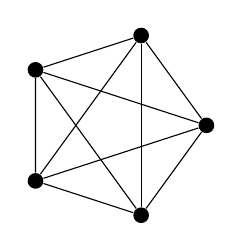
\begin{tikzpicture}[scale=0.8]
		\foreach \i in {1,...,5} {
			\node[circle,fill=black,inner sep=2pt] (v\i) at (72*\i:1.5cm) {};
		}
		\foreach \i in {1,...,5} {
			\foreach \j in {\i,...,5} {
				\ifnum \i=\j \else
				\draw (v\i) -- (v\j);
				\fi
			}
		}
	\end{tikzpicture}
	\]
\end{example}
\begin{theorem}
	\( n \) 人组成群体中，必有2个人在群体中朋友数相等。
\end{theorem}

\begin{proof}
	设 \( G=(V,E) \)，\( |V|=p=n \)。假设不存在 \( u,v \in V \) 使得 \( \deg u = \deg v \)，则顶点度数必为 \( 0,1,2,\dots,p-1 \)。
	
	但度数为 \( 0 \) 的顶点（无朋友）与度数为 \( p-1 \) 的顶点（与所有人为朋友）无法同时存在，矛盾。故必有 \( u,v \in V \) 满足 \( \deg u = \deg v \)。
\end{proof}
\begin{remark}
	这里用的不是鸽笼！！！不是！！！
\end{remark}
\begin{definition}[图同构]
	设 \( G=(V,E) \)，\( H=(U,F) \)，若存在双射 \( \varphi: V \to U \)，使得对任意 \( u,v \in V \)，有
	\[
	uv \in E \iff \varphi(u)\varphi(v) \in F
	\]
	则称 \( G \) 与 \( H \) 同构，记为 \( G \cong H \)。
\end{definition}

\begin{definition}[路和圈]
	设 \( G=(V,E) \)，\( G \) 中顶点与边的交错序列 \( v_0, x_1, v_1, x_2, \dots, x_n, v_n \)（其中 \( x_i = v_{i-1}v_i \in E \)，\( i=1,2,\dots,n \)）称为 \( G \) 的一条通路（通道），记为 \( v_0v_1v_2\cdots v_n \)（也称为 \( v_0-v_n \) 通道），\( n \) 称为通路的长度。
	
	若 \( v_0 = v_n \)，则称该通路为闭通道（回路），其长度仍为 \( n \)。
\end{definition}

\begin{remark}
	通路不重复顶点的情况称为路。
\end{remark}
\begin{remark}
	（点可以重）不重复边的情况称为迹。
\end{remark}
\begin{definition}
	闭路是圈。
\end{definition}
上面所有的概念全部都定义在无向图上了，但是当然的，它们全部都可以定义在有向图上。
\begin{remark}
	\(u\) 到 \(u \) 有长度为0的路。
\end{remark}
\begin{definition}
	图 \( G=(V,E) \) 中，若 \( \forall u,v \in V \) ， \( u,v \) 间有路，则称 \( G \) 为连通图。
\end{definition}
\begin{definition}[极大连通子图]
	（为了证底下那个定理引入极大连通子图的概念）
	
	设 \( \sim\ \subseteq V \times V \)，\( \forall u,v \in V \)，\( u \sim v \iff u,v \) 间有路。
	记 \( V/\sim = \{v_1,v_2,\dots,v_k\} \)，\( V \) 的导出子图记为 \( \langle V_i \rangle = (V_i, \mathscr{P}(V_i) \cap E) \)，称为 \( G \) 的连通分支（极大连通子图）。
\end{definition}
怎么说呢，其实就是对于每一个 \(V_i\) 找了个等价类，只不过这关系用的是能否连出来一个路。这里面的极大当然取的不是最大的含义。
\begin{theorem}
	\( G=(V,E) \) 为 \( p \) 阶图，若 \( \forall u,v \in V \)，\( u,v \) 不邻接时，有
	\[
	\deg u + \deg v \geq p-1
	\]
	则 \( G \) 连通。
\end{theorem}
\begin{proof}
	反证：设 \( G \) 不连通，则 \( G \) 至少有2个分支。设 \( G_1=(V_1,E_1) \) 为其中一个分支，其余分支为 \( G_2=(V_2,E_2) \)，\( |V_1|=n \)，\( |V_2|=p-n \)。
	
	取 \( u \in V_1 \)，则 \( \deg u \leq n-1 \)；取 \( v \in V_2 \)，则 \( \deg v \leq (p-n)-1 \)。
	
	故 \( \deg u + \deg v \leq (n-1)+(p-n-1)=p-2 \)，与 \( \deg u + \deg v \geq p-1 \) 矛盾。因此 \( G \) 连通。
\end{proof}
\begin{proof}[也能用归纳法去证明]
	注意！！！！！！这个证明有问题！！！！不用看了，或者看一眼错哪了就行！！！！
	分析：\\
	① 当 \( p=1 \) 时，结论成立；\\
	② 假设 \( p-1 \) 个顶点的图满足条件时结论成立，再证 \( p \) 个顶点的情况。\\
（是第二数学归纳法！！！）
	\begin{enumerate}
		\item \(deg(w)=0\) ，那其他点度数最大也就只有 \(p-2\) 矛盾。
		\item \(deg(w)=p-1\) ，\(G\) 显然连通了（因为我这都有一个点和所有点连接了）
		\item \(deg(w)\in[1,p-2]\) ，分析子图 \( G-w \) ，并且 \(\forall u,v\in V\setminus w\)：
		\begin{enumerate}
			\item 如果 \(uv\in E\) ，那 \(u,v\) 间有路。
			\item 如果 \(uv\notin E\) :
			\begin{enumerate}
				\item \(uw,wv\in E\) ，\(u,v\) 间有路；
				\item \(uw\notin E \) 或者 \(vw\notin E\):（问题出在这里，我需要讨论两个边是否都不在，这样删完了实际上边数就不够了，推导不下去了。）
				在 \(G-w\)中，\(deg{u}+deg(v)\geq (p-1)-1=p-2\) （本来应该是大于等于 \(p-1\) 的，删了至少一个边，就这样了），由归纳假设， \(G-w\) 应连通。
			\end{enumerate}
		\end{enumerate}
		哎总之在这个情况下，我们利用归纳假设等等乱七八糟的说明了 \(G-w\) 应该是连通的，然后 \(w\) 至少和一个点连起来了，整张图就应该是连通的。
	\end{enumerate}
	
	
	总之证明有问题，批判学习就行。
\end{proof}
	
	\begin{ap}
		如果 \( u,v \in V \) 满足 \( uv \notin E \)
		
		此时 \(\exists w\in V,\ s.t.\ uw\in E,vw\in E\)，那自然连通。
		不然，也就是说没有这样一个 \(w\) 让 \(u,v\) 去连接起来。
		
		令 \( \deg u = k \)，则 \( v \) 的邻点只能来自 \( V \setminus (\{u\} \cup \Gamma(u)) \)，（\(\Gamma\) 是相邻点的意思）故
		\[
		\deg v \leq p - 2 - k
		\]
		因此
		\[
		\deg u + \deg v \leq k + (p-2 -k) = p-2
		\]
		与题设 \( \deg u + \deg v \geq p-1 \) 矛盾。故反设不成立，结论得证。
	\end{ap}
	其实看得出来，这条件还是太强了，我们甚至直接证出来了下面这个推论：
	\begin{corollary}
		满足上述条件的图 \( G \) 任意两点距离不超过2。
	\end{corollary}
	但是我们又很容易构造出来如果不满足这个条件确实不成立。

\begin{theorem}
	设 \( G=(V,E) \) 是无向图，至少一个顶点的度不是 0 ，且任何一个顶点的度数全是偶数，那么图 \(G\) 里存在圈。
\end{theorem}

\begin{proof}
	取 \( G \) 中最长路 \( v_1,v_2,\dots,v_m \)，则 \( v_1 \) 的邻点均在该路中（如果不这样，因为 \(v_1\) 已经是一个端点，所以这个路肯定会更长），这样我把它们记成 \(v_{i_1},v_{i_2}\dots v_{i_m}\)。是所有和 \(v_1\) 相连的点。且我们知道 \(\delta\geq m\geq 2\) 和 \(i_1=2\) （因为 \(v_1\) 和 \(v_2\) 连接了）这样 \(i_m\geq m+1\).
	然后就有：
	\[v_1v_2\dots v_{i_m}x_1\]
	是一个圈（大小是 \(m+1\) ）
\end{proof}


\begin{definition}[可达关系]
	设 \( D=(V,A) \) 是有向图，若存在从 \( u \) 到 \( v \) 的有向路，则称 \( u \) 可达 \( v \)，记为 \( u R v \)。
\end{definition}

\begin{remark}
	有向图的可达关系满足：
	\begin{enumerate}
		\item 自反性：\( \forall u \in V \)，\( u R u \)；
		\item 传递性：若 \( u R v \) 且 \( v R w \)，则 \( u R w \)。
	\end{enumerate}
\end{remark}
\begin{definition}
	互达：就是 \(u\) 可达 \(v\) ，而且 \(v\) 也可达 \(u\)。
\end{definition}
\begin{remark}
	你可以用互达关系搞出来一个导出子图：
	\[<V_i>=(V_i,A\cap (V_i\times V_i\setminus \{\{u,u\}|u\in V_i\}))\]
\end{remark}
\begin{definition}[强连通]
	\( \forall u,v \in V \)，\( u v   \) 互达，则 \( D \) 是强连通图。
\end{definition}

\begin{definition}[单向连通]
	\( \forall u,v \in V \)，\( u R v \) 或 \( v R u \)，则 \( D \) 是单向连通图。
\end{definition}

\begin{definition}[弱连通]
	忽略有向边方向后，对应的无向图连通，则 \( D \) 是弱连通图。
\end{definition}
\begin{definition}
	不连通：补上也没救了，根本没边。
\end{definition}
\begin{theorem}
	\( D \) 强连通 \( \iff \)  \(  D \) 有生成闭通道。
\end{theorem}

\begin{definition}[DAG]
	有向无环图（Directed Acyclic Graph, DAG）是不含有向圈的有向图。
\end{definition}

\begin{theorem}
	设 \( D=(V,A) \) 是有向图，则：
	
	① 若 \( D \) 是DAG，则至少有一个入度为0的顶点（最长路法，拓扑排序）；
	
	② \( D \) 没有有向圈 \( \iff D \) 的任一有向通道全是有向路；
	\( \Rightarrow \)：若有有向圈，则 \( D \) 存在不是有向路的有向通道（反证）；
	\( \Leftarrow \)：（略）
	
	③ \( D \) 有有向圈 \( \iff D \) 有子图 \( D_1=(V_1,A_1) \)，使得 \( \forall v \in V_1 \)，\( id(v)>0 \) 且 \( od(v)>0 \)（最长路法）；
	
	④ 若 \( D \) 连通，且 \( \forall v \in V \)，\( od(v)=1 \)，则 \( D \) 恰有一个有向圈（反证：不然存在顶点出度为2）。
\end{theorem}

\section{补图，双图（二分图）}
\begin{definition}[补图]
	设无向图 \( G = (V, E) \)，定义 \( G \) 的补图为 \( G^c = (V, E^c) \)，其中边集 \( E^c = \mathcal{P}_2(V) \setminus E \)（\( \mathcal{P}_2(V) \) 表示 \( V \) 中元素的所有二元子集构成的集合）。
\end{definition}
\begin{remark}
	完全图 \( K_p \) 去掉图 \( G \) 的边集后得到的图即为 \( G \) 的补图（对应 \( \mathcal{P}_2(V) \setminus E \) 的定义）。
\end{remark}

\begin{definition}[有向补图]
	设有向图 \( D = (V, A) \)，定义 \( D \) 的补图为 \( D^c = (V, A^c) \)，其中弧集 \( A^c = (V \times V \setminus \{ (v, v) \mid v \in V \}) \setminus A \)。
\end{definition}

\begin{remark}
	补图与原图的边/弧满足：
	\begin{itemize}
		\item 对无向图：\( uv \in E^c \iff uv \notin E \)；
		\item 对有向图：\( uv \in A^c \iff uv \notin A \)。
	\end{itemize}
\end{remark}

\begin{remark}
	连通图的补图不一定连通，反之不连通图的补图肯定是连通的。例如：
	\begin{center}
		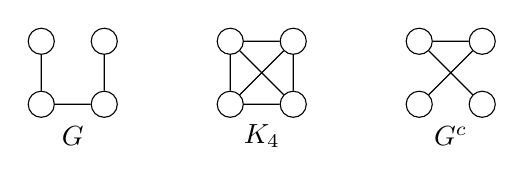
\begin{tikzpicture}[scale=0.8]
			% 图G
			\node (a1) at (0,1) [circle, draw] {};
			\node (a2) at (1,1) [circle, draw] {};
			\node (a3) at (1,0) [circle, draw] {};
			\node (a4) at (0,0) [circle, draw] {};
 			\draw (a1)--(a4)--(a3)--(a2);
			\node at (0.5,-0.5) {$G$};
			
			% 完全图K4
			\node (b1) at (3,1) [circle, draw] {};
			\node (b2) at (4,1) [circle, draw] {};
			\node (b3) at (4,0) [circle, draw] {};
			\node (b4) at (3,0) [circle, draw] {};
			\draw (b1)--(b2)--(b3)--(b4)--(b1);
			\draw (b1)--(b3);
			\draw (b2)--(b4);
			\node at (3.5,-0.5) {$K_4$};
			
			% 补图G^c
			\node (c1) at (6,1) [circle, draw] {};
			\node (c2) at (7,1) [circle, draw] {};
			\node (c3) at (6,0) [circle, draw] {};
			\node (c4) at (7,0) [circle, draw] {};
			\draw (c1)--(c4);
			\draw (c2)--(c3);
			\draw (c1)--(c2);
			\node at (6.5,-0.5) {$G^c$};
		\end{tikzpicture}
	\end{center}
\end{remark}



\begin{theorem}
	若图 \( G \cong H \)（\( G \) 与 \( H \) 同构），则其补图满足 \( G^c \cong H^c \)。
\end{theorem}

\begin{definition}[自补图]
	若图 \( G \cong G^c \)，则称 \( G \) 为自补图。自补图的顶点数 \( p \) 满足 \( q=p(p-1)/4 \)
\end{definition}

\begin{theorem}[Ramsey定理（补图形式）]
	设 \( G = (V, E) \) 是6顶点图，则 \( G \) 中存在三角形，或其补图 \( G^c \) 中存在三角形。
\end{theorem}

\begin{definition}[双图（偶图）]
	设图 \( G = (V, E) \)，若存在顶点集的划分 \( V = V_1 \cup V_2 \)（满足 \( V_1 \cap V_2 = \varnothing \) 且 \( V_1, V_2 \neq \varnothing \)），使得对任意 \( uv \in E \)，有 \( u \in V_1, v \in V_2 \) 或 \( u \in V_2, v \in V_1 \)，则称 \( G \) 为双图（或偶图）。
\end{definition}

\begin{definition}[距离]
	设图 \( G = (V, E) \)，对任意 \( u, v \in V \)，定义 \( u, v \) 间的距离 \( d(u, v) \) 为 \( u \) 到 \( v \) 的最短路径长度；若 \( u, v \) 间无路径，则 \( d(u, v) = +\infty \)。
\end{definition}

\begin{theorem}[偶图的判定]
	图 \(G\) 是偶图 \(\iff\) 所有圈的长度均为偶数。
\end{theorem}
\begin{proof}
	（必要条件）二分图里面的一个圈是 \(v_1v_2\dots v_n v_1\)， 因为任何一个边的两端肯定在两个点集里（二分图定义），所以可以知道（先假设 \(v_1\in V_1\) ）所有下标是偶数的点肯定全在 \(V_2\) 里，又因为 \(v_nv_1\in E\)，所以这个 \(n\) 肯定是偶数，也就是这个圈的长度是偶数。
	
	（充分条件）首先取一个 \(u\in V\) 然后记 \(V_1=\{v|d(u,v)\ is\ even\},V_2=V\setminus V_1\) ，这已经完成了二分图的构造，接下来反证，假设 \(w,v\in V_1\ and\ wv\in E\)，那么一定会构造出来一个奇数圈（这是很好验证的），因此一定不存在 \(V_1\) 集合内的连边。
	然后考虑全部在 \(V_2\) 里的两个点，可以发现基本同理，证毕。
\end{proof}

\begin{definition}[完全二分图 \( K_{m,n} \)]
	设图 \( G = (V, E) \) 的顶点集划分为 \( V = V_1 \cup V_2 \)（\( V_1 \cap V_2 = \varnothing \)），若 \( |V_1| = m \)、\( |V_2| = n \)，且任意 \( u \in V_1, v \in V_2 \) 均满足 \( uv \in E \)，则称 \( G \) 为完全二分图，记为 \( K_{m,n} \)。
	
	其边数为 \( |E| = m \cdot n \)，且 \( K_{n,n} \) 是顶点数为 \( m+n \)恒定（当然必须是个偶数）、边数为 \( mn \) 的图中，边数最多的图（均值不等式保证了这一点）。
\end{definition}

\begin{theorem}[Turán定理（无 \( K_3 \) 情况）]
	设 \( G = (V, E) \) 是顶点数为 \( p \)、边数为 \( q \) 的图，若 \( G \) 中无三角形（即不含子图 \( K_3 \)），则：
	\[
	q \leq \left\lfloor \frac{p^2}{4} \right\rfloor
	\]
\end{theorem}
\begin{proof}[归纳法证明（以 \( p \) 为奇数为例）]
	\begin{enumerate}
		\item \( p = 1, 2, 3 \) 时，直接验证结论成立。
		\item 归纳假设（先对奇数情况进行归纳）：设 \( p = 2n-1 \) 时结论成立，即无三角形的 \( (2n-1, q') \) 图满足 \( q' \leq \left\lfloor \frac{(2n-1)^2}{4} \right\rfloor = n^2 - n \)。
		\item 归纳步骤：考虑 \( p = 2n+1 \) 的无三角形图 \( G = (V, E) \)，任取边 \( uv \in E \)，记 \( G' = G - u-v \)（移除点 \( u,v \) 后的图）。
		\( G' \) 是顶点数为 \( 2n-1 \) 的无三角形图，由归纳假设，\( G' \) 的边数 \( q' \leq n^2 - n \)。
		
		然后考察一下去掉的这两个点，假设 \(deg(u)=k\)，那 \(deg(v)\leq 2n+1-k\)，这是因为在原来这 \(2n+1\) 个点里， \(v\) 不能连接 \(u\) 已经连接过的点了，所以去掉之后应该一共最多去掉了 \(2n+1-k+k-1=2n\) 条（因为 \(uv\) 连边计算了两次）
		
		原边数 \( q \leq q' + 2n=n^2+n \)得：
		\[
		q \leq \left\lfloor \frac{(2n+1)^2}{4} \right\rfloor
		\]
	\end{enumerate}
	故结论对所有正整数 \( p \) 成立。
\end{proof}
\begin{theorem}
	无三角形的 \( k \)-正则图至少含有 \( 2k \) 个顶点。
\end{theorem}

\begin{proof}[构造性证明]
	（哦对当然 \(k=1\) 的情况很简单，验证下就行，直接考虑 \(k>1\) ）构造两个相连的顶点 \( u, v \)，使 \( u \) 连接 \( k-1 \) 个不同顶点，\( v \) 也连接 \( k-1 \) 个不同顶点（且与 \( u \) 连接的顶点不重复），则总顶点数为 \( 2 + 2(k-1) = 2k \)。
	用图示意如下：

\begin{center}
	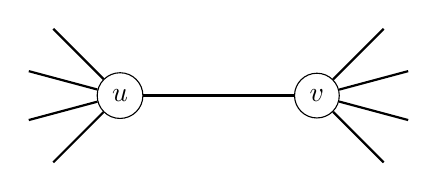
\begin{tikzpicture}
		% 中心节点：u在左(0,0)，v在右(2.5cm,0)，间距拉大更清晰
		\node (u) [circle, draw, minimum size=8pt] at (0,0) {$u$};
		\node (v) [circle, draw, minimum size=8pt] at (2.5,0) {$v$};
		\draw[thick] (u) -- (v); % u-v连线加粗
		
		% 核心参数（直观易懂，可直接改）
		\def\k{4}       % 每个节点的发散边数（3=上/中/下三个方向）
		\def\angle{45}  % 上下发散角度（45°=更开，视觉更明显）
		\def\len{1.2cm} % 边的长度（更长，避免拥挤）
		
		% ---------------------- u 向左发散（纯左侧方向）----------------------
		% 角度：135°(左上)、180°(正左)、225°(左下)，完全在u的左侧
		\foreach \i in {1,...,\k} {
			\pgfmathsetmacro{\ang}{180 - \angle + (\angle*2/(\k-1))*(\i-1)}
			\draw[thick] (u) -- ++(\ang:\len); % ++表示从u出发向外延伸
		}
		
		% ---------------------- v 向右发散（纯右侧方向）----------------------
		% 角度：45°(右上)、0°(正右)、315°(右下)，完全在v的右侧
		\foreach \i in {1,...,\k} {
			\pgfmathsetmacro{\ang}{0 + \angle - (\angle*2/(\k-1))*(\i-1)}
			\draw[thick] (v) -- ++(\ang:\len); % ++确保从v出发向外延伸
		}
	\end{tikzpicture}
\end{center}

	因此无孤立点的 \( k \)-正则图至少有 \( 2k \) 个顶点。
\end{proof}


\section{Euler 图和 Hamilton 图}

\subsection{Euler 图}
\begin{definition}[Euler闭迹]
	设图 \( G = (V, E) \)，若 \( G \) 中存在一条闭迹，包含 \( G \) 的所有顶点与所有边，则称该闭迹为 \( G \) 的 Euler 闭迹。
\end{definition}

\begin{definition}[欧拉图]
	若图 \( G \) 存在Euler闭迹，则称 \( G \) 为\textbf{欧拉图}。
\end{definition}

\begin{theorem}[Euler 图判定定理]
	图 \( G = (V, E) \) 是欧拉图的充要条件是：
	\( G \) 连通，且对任意 \( v \in V \)，顶点 \( v \) 的度数为偶数（即 \( \deg v = 2k, k \in \mathbb{N}^* \)）。
\end{theorem}

\begin{proof}
	\("\Rightarrow"\) 显然（有进边肯定也有出边）
	
	\("\Leftarrow"\) “连圈成迹”（建议看教材，这挺神秘的）
\end{proof}
\begin{theorem}[Euler开迹判定]
	图 \( G = (V, E) \) 存在Euler开迹（非闭，起点≠终点）的充要条件是：
	\( G \) 连通，且 \( G \) 中恰有2个奇度顶点。
\end{theorem}

\begin{theorem}[开迹覆盖数]
	若连通图 \( G \) 有 \( 2n \) 个奇度顶点，则 \( G \) 的开迹覆盖数为 \( n \)（即需 \( n \) 条开迹覆盖所有边）。
\end{theorem}
上面两个定理的证明可以看《集合论与图论》164页到155页。


上述结论对伪图（允许环、重边）同样成立；
求Euler迹的常用算法：Fleury算法、深度优先搜索（DFS）回溯法。不进一步展开了。


\subsection{Hamilton 图}
\begin{definition}[哈密顿图]
	设图 \( G = (V, E) \)，若 \( G \) 中存在一个包含所有顶点的圈（闭通路），则称 \( G \) 为哈密顿图；包含所有顶点的路称为哈密顿路。
\end{definition}
必要性判定：染色法（略）

哈密顿图需满足以下必要条件：
\begin{enumerate}
	\item 顶点数 \( p \geq 3 \) 且图连通；
	\item 若顶点 \( v \) 的度数 \( \deg v = 2 \)，则 \( v \) 的两条关联边必在哈密顿圈上；
	\item 若顶点 \( v \) 的度数 \( \deg v = 3 \)，则 \( v \) 的三条关联边中一定只有两条在哈密顿圈上；
	\item 哈密顿圈的一部分不能是圈。
	\item 没有桥或者割点。
\end{enumerate}

\begin{theorem}
	设 \( G = (V, E) \) 是哈密顿图，则对任意非空顶点子集 \( S \subseteq V \)（\( S \neq \varnothing \)），有：
	\[
	\omega(G - S) \leq |S|
	\]
	其中 \( \omega(G ) \) 表示图 \( G \) 的连通分支数。
\end{theorem}

\begin{proof}
	设 \( H \) 是 \( G \) 中的哈密顿圈，对任意非空 \( S \subseteq V \)：
	\begin{enumerate}
		\item 对圈 \( H \)，移除 \( n \) 个顶点后，连通分支数最多增加 \(n-1\) 个。 \( \omega(H - S) \leq |S| \)；
		\item 由于 \( H \subseteq G \)，故 \( \omega(G - S) \leq \omega(H - S) \)；
		\item 因此 \( \omega(G - S) \leq |S| \)。
	\end{enumerate}
\end{proof}

\begin{remark}
	该条件是哈密顿图的必要条件（不满足则一定非哈密顿图），但不是充分条件（满足条件的图不一定是哈密顿图）。
\end{remark}


接下来是一些充分条件，也就是 Dirac 定理和 Ore 定理。

\begin{theorem}[Dirac 定理]
	设 \( G = (V, E) \) 是顶点数 \( p \geq 3 \) 的简单图，若对任意 \( v \in V \)，有 \( \deg v \geq \frac{p}{2} \)，则 \( G \) 是哈密顿图。
\end{theorem}

\begin{proof}[反证法（证逆否命题）]
	需证：若 \( G \) 是 \( p \geq 3 \) 的非哈密顿图，则存在 \( u \in V \) 使得 \( \deg u < \frac{p}{2} \)。

	首先构造极大非哈密顿图
	设 \( G \) 是非哈密顿图，在 \( G \) 的不相邻顶点间添加边，只要没得到 Hamilton 图就一直加，最后得到一张极大非哈密顿图 \( G^* \)（再添边则 变成哈密顿图）。
	
	取极大非 Hamilton 图的 Hamilton 路 \( P = v_1v_2\cdots v_p \)。
	记 \( \deg_{G^*}(v_1) = k \)，\( v_1 \) 的邻点为 \( \{v_{i_1}, \dots, v_{i_k}\} \)。
	由于 \( G^* \) 非哈密顿图，\( v_p \) 不能与 \( \{v_{i_1-1}, \dots, v_{i_k-1}\} \) 相邻（否则构造哈密顿圈）。
	

	由上述分析，\( v_p \) 的邻点不能包含 \( \{v_{i_1-1}, \dots, v_{i_k-1}\} \)，故：
	\[
	\deg_{G^*}(v_1) \leq (p-1) - k
	\]
	即 \( \deg_{G^*}(v_1) + \deg_{G^*}(v_p) \leq p-1 \)。
	
	若 \( G \) 中所有顶点度数 \( \geq \frac{p}{2} \)，则 \( \deg_{G^*}(v_1) + \deg_{G^*}(v_p) \geq p \)，与上式矛盾。
	因此 \( G \) 中必存在顶点 \( u \)，使得 \( \deg u < \frac{p}{2} \)。
	
	
	\medskip
	逆否命题成立，故原定理得证。
\end{proof}

仿照证明思路可以一模一样的干出来 Ore 定理：

\begin{theorem}[Ore 定理]
	设 \( G = (V, E) \) 是顶点数 \( p \geq 3 \) 的简单图，若对任意不相邻顶点 \( v,u \in V \)，有 \( deg (v) + deg (u) \geq p \)，则 \( G \) 是哈密顿图。
\end{theorem}

还能得到点别的：
\begin{theorem}
	设 \( G = (V, E) \) 是 \((p,q)\) 图，若对任意不相邻顶点 \( v,u \in V \)，有 \( deg (v) + deg (u) \geq p-1 \)，则 \( G \) 有哈密顿路。
\end{theorem}
\begin{proof}
	P157
\end{proof}

\section{比赛图}
\begin{definition}[比赛图]
	设 \( D = (V, A) \) 是 \( (p,q) \) 有向图，若对任意 \( u, v \in V \)（\( u \neq v \)），\( (u,v) \in A \) 与 \( (v,u) \in A \) 有且仅有一个成立，则称 \( D \) 为\textbf{比赛图}。
	
	比赛图是完全图 \( K_p \) 的定向图，对应“循环赛（两两分胜负）”的数学模型。
\end{definition}
\begin{definition}
	\(od(v)\) 称为 \(v\) 的分数。
\end{definition}
\begin{theorem}
	任一比赛图中必存在一条有向哈密顿路。
\end{theorem}

\begin{proof}
	（最长路法）
	设比赛图 \( D \) 的最长有向路为 \( P: v_1v_2\cdots v_k \)。
	
	若 \( k = p \)，则 \( P \) 是有向哈密顿路，结论成立。
	
	若 \( k < p \)，则存在顶点 \( v \notin P \)。
	\\
	若 \( P \) 中无顶点指向 \( v \)，则 \( vv_1v_2\cdots v_k \) 是更长的路，与 \( P \) 是最长路矛盾；\\
	若 \( P \) 中存在顶点指向 \( v \)，取最后一个指向 \( v \) 的顶点 \( v_i \)，则 \( v_1\cdots v_ivv_{i+1}\cdots v_k \) 是更长的路，亦与 \( P \) 是最长路矛盾。
	
	因此 \( k = p \)，即 \( P \) 是有向哈密顿路。
\end{proof}


\begin{proof}
	施归纳于比赛图的顶点数 \( p \)：\\
    \( p=1,2 \) 时，显然存在有向哈密顿路。\\
	归纳假设：设 \( p \) 个顶点的比赛图存在有向哈密顿路。\\
	归纳步骤：
	对 \( p+1 \) 个顶点的比赛图 \( D \)，去掉一个顶点 \( v \) 得 \( D-v \)。由归纳假设，\( D-v \) 有哈密顿路 \( P: v_1v_2\cdots v_p \)。
	
	若 \( P \) 中无顶点指向 \( v \)，则 \( vv_1v_2\cdots v_p \) 是 \( D \) 的哈密顿路；
	
	若 \( P \) 中存在顶点指向 \( v \)，取最后一个指向 \( v \) 的顶点 \( v_i \)，则 \( v_1\cdots v_ivv_{i+1}\cdots v_p \) 是 \( D \) 的哈密顿路。
	
	综上，结论对所有 \( p \geq 1 \) 成立。
\end{proof}

两个证明其实差不多（）


其他内容我过两天更新。

\section{带权图，邻接表，邻接矩阵}
Dijkstra 算法和 Floyd 算法看书吧。大概理解下思路，后面需要的话会补的。





\chapter{树}
\section{树的基本概念}

\begin{definition}
	（树）连通无圈的无向简单图称为\textbf{树（tree）}。
\end{definition}

\begin{definition}
	无圈的无向简单图称为\textbf{森林（forest）}。
\end{definition}

\begin{definition}
	只有一个顶点的图称为平凡树。
\end{definition}

\begin{definition}
	对于一个树上的点 \(u\) ，如果 \(deg(u)=1\) ，那 \(u\) 称作叶子。 
\end{definition}
\begin{definition}
	顶点个数称为树的阶。
\end{definition}

\begin{definition}
	连通森林是树，当然，树也是森林（
\end{definition}

\begin{theorem}
	非平凡树（顶点数 \( \geq 2 \)）至少有两个叶子。
\end{theorem}

\begin{proof}
	找到树上的最长路，易知道它的两端应该全是叶子。
\end{proof}

\begin{theorem}
	树是二分图。
\end{theorem}
\begin{proof}
	也可以用染色法证明，（后面会证明）树的中心或者是一个顶点，或者是两个邻接的顶点。
	从树的中心开始染色：如果树的中心是一个顶点，则将其染为红色；如果树的中心是两个顶点，则将它们中的一个染为红色，另一个染为蓝色。
	然后按照如下的规则逐层为树的其他顶点染色：如果顶点 \( u \) 和 \( v \) 邻接，且 \( u \) 已经染了红色或蓝色中的一种颜色，则将 \( v \) 染为红色或蓝色中的另一种颜色。
	这样逐层进行，可以得到树的一种2-顶点着色，对应着顶点的一个2-划分，每条边的两个端点都在不同的划分块中，所以是二部图。
\end{proof}
\begin{ap}
	树是无圈图，所有圈的大小是 \(0\)，由前定理知树是二分图。
\end{ap}
\begin{theorem}
	设 \( G \) 是无向简单图，以下命题等价：
	\begin{enumerate}
		\item \( G \) 是树；
		\item 对任意 \( u, v \in V(G) \)，\( u \) 与 \( v \) 之间有且仅有一条路径；
		\item \( G \) 连通且 \( p = \)  \( q + 1 \)；
		\item \( G \) 无圈且 \( p = q + 1 \)；
		\item \( G \) 无圈，任意不相邻的两个点之间添加一条边后会形成唯一的圈。
	\end{enumerate}
\end{theorem}

\begin{proof}
	\( (2) \Rightarrow (3) \)（数学归纳）：\\
	当 \( p=1 \) 时，\( q=0 \)，满足 \( p = q + 1 \)，成立。\(p=2\) 的时候也容易验证；\\
	假设 \( p<k \) 时全部成立（第二数归），当 \( p=k \) 时，因为任意两个点之间的路唯一，所以任取一条边 \( e \)，删除 \( e \) 后 \( G \) 分为两个子树 \( G_1, G_2 \)，设 \( G_1 \) 顶点数为 \( p_1 \)、边数为 \( q_1 \)，\( G_2 \) 顶点数为 \( p_2 \)、边数为 \( q_2 \)。
	由归纳假设，\( p_1 = q_1 + 1 \)，\( p_2 = q_2 + 1 \)。
	则 \( p = p_1 + p_2 = (q_1 + 1) + (q_2 + 1) = (q_1 + q_2+1) + 1 \)，成立。
	
	\( (3) \Rightarrow (4) \)：
	反证法，若 \( G \) 有圈，删除圈中一条边后 \( G \) 仍连通，此时 \( p = q \)，与 \( p = q + 1 \) 矛盾，故 \( G \) 无圈。
	
	\( (3) \Rightarrow (5) \)：
	\( G \) 无圈，任取不相邻的两点 \( u, v \)，添加边 \( (u, v) \)，由 \( (2) \) 知原树中 \( u, v \) 有唯一路径，添加边后形成唯一的圈。


	\( (4) \Rightarrow (3) \)：
	设图 \( G \) 不连通，有 \( k \) 个连通分支（\( k \geq 2 \)），记第 \( i \) 个连通分支为 \( G_i \)（顶点数 \( p_i \)，边数 \( q_i \)）。
	由整个图没圈，子图肯定也没有圈，所以应用 \((4)\)， 对每个 \( G_i \) 有 \( p_i = q_i + 1 \)。
	因此总顶点数 \( p = \sum_{i=1}^k p_i = \sum_{i=1}^k (q_i + 1) = q + k \)（\( q = \sum_{i=1}^k q_i \) 为总边数）。
	因为 \( G \) 无圈，则 \( p = q + 1 \)，故 \( k = 1 \)，矛盾。因此树必连通。
\end{proof}

\begin{definition}
	（极小连通图）若图 \( G \) 去掉任意一条边后不连通，则称 \( G \) 为极小连通图。
\end{definition}

\begin{theorem}
	图 \( G \) 是极小连通图当且仅当 \( G \) 是树。
\end{theorem}

\begin{proof}
	trivial.
\end{proof}
以下的几个定义设连通图 \( G = (V, E) \)，且是对顶点 \( v \in V \) 讨论的。
\begin{definition}
	\( e(v) = \max_{u \in V} d(u, v) \) 称为 \( v \) 的偏心率。
\end{definition}
\begin{definition}
	\( r(G) = \min_{v \in V} e(v) \) 称为 \( G \) 的半径。
\end{definition}
\begin{definition}
	\( d(G) = \max_{v \in V} e(v) \) 称为 \( G \) 的直径。
\end{definition}
\begin{definition}
	满足 \( e(v) = r(G) \) 的顶点 \( v \) 称为 \( G \) 的中心点，所有中心点的集合称为 \( G \) 的中心。
\end{definition}

\begin{theorem}
	若 \( T \) 是树，则 \( T \) 的中心恰有1个顶点或2个相邻顶点。
\end{theorem}

\begin{proof}[教材P173]
	采用数学归纳法，施归纳于树T的阶 \(p\).
	
	显然，\(p=1,2\) 时结论成立.
	
	假设对 \(p<k (k \geq 3)\) 阶树结论成立，设 \(T\) 为 \(k\) 阶树，删掉 \(T\) 的所有叶子得到的树 $T'$ 中，每个顶点的偏心率比它们在 \(T\) 中的偏心率少 \(1\) .又因为 \(T\) 的叶子不能是中心点，所以 \(T\) 的中心点在$T'$中。如果某个顶点 \(w\) 的偏心率在 \(T\) 中最小，则在$T'$中依然是最小的，故 \(T\) 与 $T'$ 的中心相同。因为 $T'$ 的阶小于k，由归纳假设， $T'$ 的中心(也是 \(T\) 的中心)或为一个顶点，或为 \(2\) 个相邻接的顶点。
	\end{proof}
\begin{theorem}
	设树中度数为 \( i \) 的顶点个数为 \( n_i \)，则有：
	\[
	\sum_{i=1}^k n_i = p
	\]
	\[
	n_1 = 2 + n_3 + 2n_4 + \dots + (k-2)n_k
	\]
	其中 \( p \) 为树的顶点数（阶）。
\end{theorem}

\begin{proof}
	\[
	\sum_{i=1}^k i \cdot n_i = 2q = 2(p - 1)
	\]
	将 \( p = \sum_{i=1}^k n_i \) 代入上式：
	\[
	\sum_{i=1}^k i \cdot n_i = 2\left(\sum_{i=1}^k n_i - 1\right)
	\]
	展开整理后可得：
	\[
	n_1 = 2 + n_3 + 2n_4 + \dots + (k-2)n_k
	\]
\end{proof}

\section{生成树}

\begin{definition}[生成树]
	设图 \( G = (V, E) \)，若 \( T \) 是包含 \( G \) 所有顶点的子图且 \( T \) 为树，则称 \( T \) 是 \( G \) 的生成树。
\end{definition}

\begin{theorem}
	图 \( G \) 存在生成树的充要条件是 \( G \) 连通。
\end{theorem}

\begin{theorem}
	若 \( G \) 连通且 \(q\geq p-1 \)，则 \( G \) 有生成树。
\end{theorem}


\subsection{生成树计数方法}
生成树的计数方法主要包括：
\begin{enumerate}
	\item Cayley递推法
	\item 关联矩阵法\\
	设 \( A = (a_{ij}) \) 是图 \( G \) 的关联矩阵，其中元素定义为：
	\[
	if\ e_k=v_iv_j\in E,
	\begin{cases}
		a_{ik}=1 \\
		a_{kj}=-1 \\
		a_{lk}=0\ if\ l\neq i\ and\ l\neq j.
	\end{cases}
	\]
	记 \( C = A \cdot A^T \)，则 \( C \) 的 \( p-1 \) 阶主子式的绝对值等于 \( G \) 的生成树数量。
	\item 矩阵树定理
	\item Prüfer序列法
\end{enumerate}


\subsection{生成树算法}
常见的生成树（最小生成树）算法及时间复杂度：
\begin{enumerate}
	\item Kruskal 算法：时间复杂度 \( O(p\log p) \)
	\item 管梅谷破圈法：时间复杂度 \( O(p^3) \)
	\item Prim 算法：时间复杂度 \( O(p^2) \)
	\item Sollín 算法 （并行计算）
\end{enumerate}

\section{有根树与有序树}

\begin{definition}
	没有弱圈的弱连通有向图称作有向树。
\end{definition}

\begin{definition}
	若有向树中存在唯一顶点 \( u \) 满足 \( id(u) = 0 \)，且对其余所有顶点 \( v \) 满足 \( id(v) = 1 \)，则称该有向树为有根树。其中：\\
	 \( id(u) = 0 \) 的顶点 \( u \) 称为根顶点；\\
	\( id(v) = 1 \) 的顶点称为内顶点。\\
	\( od(v) = 0 \) 的顶点称为叶子。
\end{definition}
\subsection{有根树的子树与节点关系}

\begin{definition}
	有根树的反向树称为入树。
\end{definition}

\begin{definition}
	根到任何一个点 \(v\) 的有向路长是 \(v\) 的深度。
\end{definition}

\begin{definition}
	一个点到叶子的最长有向路长称作这个点的高度。
\end{definition}
\begin{definition}
	顶点 \( v \) 的所有后继顶点（包括这个点自己）称为 \( v \) 的后代。特别地，直连的那个点为儿子。我们相类似的定义每个点的父亲和祖先。
\end{definition}

\begin{definition}
	有根树中，深度相同的点位于同一层。
\end{definition}


\subsection{正则树}

\begin{definition}
	若有根树 \( T \) 中存在顶点 \( u \) 满足 \( od(u) = 0 \) 或 \( od(u) = m \)，则称 \( T \) 为 \( m \)-正则树。
\end{definition}

\begin{theorem}
	高度为 \( h \) 的 \( m \)-正则树，最多有 \( m^h \) 个叶子。
\end{theorem}

\begin{theorem}
	若 \( m \)-正则树有 \( i \) 个内顶点，则其顶点总数为 \( m \cdot i + 1 \)。
\end{theorem}

\begin{corollary}
	设 \( m \)-正则树的顶点数为 \( n \)、叶子数为 \( l \)，内顶点数为 \(i\) ，则 \(n,l,i\) 知二推一。
\end{corollary}

\begin{example}
	2-正则树。
\end{example}


\subsection{有序树与二叉树}

\begin{definition}[有序树]
	若有根树 \( T \) 中每个顶点的子树均被赋予从左到右的顺序，则称 \( T \) 为有序树。
\end{definition}

\begin{example}
	表达式 \( A \times B - C / (D - E) \) 对应的语法树（有序树）结构为：
	\[
	\begin{tikzpicture}[
		% 分层级设置间距（核心修正）
		level 1/.style={sibling distance=3cm},    % 根节点“-”的两个子节点（×、⊕）间距
		level 2/.style={sibling distance=1.2cm},  % 第二层（×、⊕）的子节点间距
		level 3/.style={sibling distance=1cm},    % 第三层（-）的子节点（D、E）间距
		level distance=1.5cm                      % 层级之间的垂直距离（避免上下重叠）
		]
		\node {$- $}
		child {node {$\times$}
			child {node {$A$}}
			child {node {$B$}}
		}
		child {node {/}
			child {node {$C$}}
			child {node {$- $}
				child {node {$D$}}
				child {node {$E$}}
			}
		};
	\end{tikzpicture}
	\]
\end{example}

\begin{definition}[二叉树]
	每个顶点最多有2个儿子（通常区分左、右）的有根树称为二叉树（只有一个儿子的时候需要指明是左儿子还是右儿子）。
\end{definition}

\begin{definition}[完全二叉树]
	若二叉树的每个层（除最后一层外）均被顶点填满，且最后一层的顶点集中在左侧，则称其为完全二叉树。
\end{definition}
\begin{definition}
	（满二叉树）高为 \(h\) 而且恰好有 \(2^{h+1}-1\) 个顶点的树叫做满二叉树。
\end{definition}
\begin{remark}
	上面那个式子指明了二叉树所能具备的最多顶点数。
\end{remark}
\begin{definition}[堆]
	满足“父顶点值不大于子顶点值”的完全二叉树称为堆。
\end{definition}


\section{割点、桥、割集}
（下面定义里面出现的 \(\omega(\cdot)\) 指的是图的分支数）
\begin{definition}
	设 \( G=(V,E) \) 是一个图，\( v \in V \)。若 \( \omega(G-v) > \omega(G) \)，则称 \( v \) 是 \( G \) 的一个割点；
	设 \( e \in E \)，若 \( \omega(G-e) > \omega(G) \)，则称 \( e \) 是 \( G \) 的桥。
\end{definition}

\begin{remark}
	桥的端点不一定是割点（例如 \( K_{2} \) 中，边是桥，但两个端点都不是割点）。
\end{remark}
\begin{remark}
	如果桥的端点度数大于 1 ，那这个点肯定是割点。
\end{remark}
\begin{proof}
	略
\end{proof}
\begin{proposition}
	有割点（或桥）的图不是哈密顿图（\( H \)-图）。
\end{proposition}

\begin{remark}
	非平凡连通图中至少有2个顶点不是割点。
\end{remark}

\begin{theorem}
	设 \( G=(V,E) \) 是连通图，\( v \in V \)，则以下命题等价：
	\begin{enumerate}
		\item \( v \) 是 \( G \) 的一个割点；
		\item 存在 \( u,w \in V \)（\( u \neq w \)），使得 \( v \) 在 \( u \) 与 \( w \) 间的每条路径上；
		\item 存在 \( V\setminus\{v\} \) 的2-划分 \( \{U,W\} \)，使得对任意 \( u \in U \)、\( w \in W \)，\( v \) 在 \( u \) 与 \( w \) 间的每条路径上。
	\end{enumerate}
\end{theorem}




\begin{proof}
	\(1\Rightarrow 3\) : 若 \( v \) 是割点，则 \( G-v \) 至少有2个分支，设 \( u \in V(G_1) \)、\( w \in V(G_2) \)（\( G_1,G_2 \) 是 \( G-v \) 的两个分支）。
	若 \( G \) 中存在 \( u \) 到 \( w \) 的路径不经过 \( v \)，则该路径也是 \( G-v \) 中的路径，与 \( G_1,G_2 \) 是不同分支矛盾，故 \( v \) 在 \( u \) 到 \( w \) 的每条路径上。
	
	\(2\Rightarrow 1\) : 若 \( v \) 在 \( u \) 到 \( w \) 的每条路径上，则 \( G-v \) 中 \( u \) 与 \( w \) 不连通，即 \( \omega(G-v) > \omega(G) \)，故 \( v \) 是割点。
\end{proof}

\begin{theorem}
	设 \( G=(V,E) \) 是连通图，\( x \in E \)，则以下命题等价：
	\begin{enumerate}
		\item \( x \) 是 \( G \) 的一座桥；
		\item \( x \) 不在 \( G \) 的任何一个圈上；
		\item 存在 \( G \) 的两个不同顶点 \( u \) 和 \( w \)，使得边 \( x \) 在 \( u \) 与 \( w \) 的每条路径上；
		\item 存在 \( V \) 的一个2-划分 \( \{U,W\} \)，使得对任意 \( u \in U \)、\( w \in W \)，边 \( x \) 在 \( u \) 与 \( w \) 间的每条路径上。
	\end{enumerate}
\end{theorem}
具体证明见书P183.
\begin{definition}
	设 \( G=(V,E) \) 是一个图，\( S \subseteq E \)。若 \( \omega(G-S) > \omega(G) \)，且对任意 \( T \subset S \) 都有 \( \omega(G-T) \leq \omega(G) \)（实际上 \( \omega(G-T)=\omega(G) \)），则称 \( S \) 是 \( G \) 的一个割集。
\end{definition}

\begin{remark}
	割集的边数不一定一样，最小割指的是破坏连通程度的满足包含关系的边集中最小的那个。
\end{remark}
\begin{remark}
	若 \( |S| \geq 2 \)，则 \( S \) 中的任意一条边都不是 \( G \) 的桥。
\end{remark}

\begin{theorem}
	设 \( G=(V,E) \) 是连通图，\( S \) 是 \( G \) 的割集，则 \( \omega(G-S) = 2 \)。
\end{theorem}

\begin{remark}
	不连通图的割集一定是它某个支的割集。
\end{remark}

\begin{theorem}
	设 \( T \) 是 \( G \) 的生成树，\( S \) 是 \( T \) 的割集，则 \( S \) 与 \( T \) 至多有一条公共边（或表述为：\( G-S \) 中有 \(T\)）。
\end{theorem}

\begin{theorem}
	连通图的每个圈与割集都有偶数条公共边。
\end{theorem}

（此处省略一车例题和定理）


\chapter{连通度，匹配和覆盖}
本节的参考书目：
\begin{enumerate}
	\item 集合论与图论   \( \ \)姜守旭等.
	\item A Course in Combinatorics J.H.van Lint and R.M.Wilson.
	\item Introductory Combinatorics ( Fifth Edition ) Richard.A.Brualdi.
\end{enumerate}
\section{连通度}
\begin{definition}
	if a graph \(G=(V,E)\)。从这个图例得到了一个不连通图或者平凡图所需要从 \(G\) 里去掉的最少顶点所构成的顶点集或者边集的点（或者边）的数目称为这个图 \(G\) 的点连通度（或者边连通度，对边而言）。把这个数记成 \(\kappa(G)\ or\ \lambda(G)\)。 
\end{definition}
\begin{remark}
	一定注意可以被删成平凡图，这意味着虽然我们删去一个仅仅由两个点和一条边组成的图时，删去任何一个顶点它都不会变得不连通，但是由于已经是平凡图，我们依然承认 \(\kappa(G)=1\)。
\end{remark}
\begin{theorem}
	(Whitney's inequality)\(\kappa(G)\leq\lambda(G)\leq\delta(G)\).
\end{theorem}
Whitney 不等式需要会证明！！！而且一定要深刻的理解 \(\kappa(G)\) 的含义！

我们在这里可以构造性地给出 Whitney 不等式的更强的使用条件：如果整数 \(a,b,c\) 满足以下条件：
\[0\leq a\leq b\leq c\] 那么我们可以找到一张图，使得：
\[\kappa(G)=a,\lambda(G)=b,\delta(G)=c.\]
下面这个定理书上写的比较防御性证明，感谢 @闪灵头上长夜莺丷 清晰而简洁的讨论阐明了证明的细节。
\begin{theorem}
	设 \( G = (V, E) \) 是平面图，若 \( \delta\bigl(G\bigr) \geq \left\lfloor \frac{|V|}{2} \right\rfloor \)，则 \( \lambda\bigl(G\bigr) = \delta\bigl(G\bigr) \)。
\end{theorem}

\begin{proof}
	（在此只选择书上证法二）
	因为 \( \lambda\bigl(G\bigr) \leq \delta\bigl(G\bigr) \)，因此仅需说明 \( \delta\bigl(G\bigr) \leq \lambda\bigl(G\bigr) \) 即可。
	
	将 \( \lambda\bigl(G\bigr) \) 条边删去，我们可得到两个子图 \( G_1, G_2 \)。
	
	记 \( G_1 \) 中的顶点为 \( u \)，自然满足 \( \deg_G u \geq \delta\bigl(G\bigr) \)。
	\[
	\delta\bigl(G\bigr) \leq \deg_G u = \deg_{G_1} u + \deg_{G_2} u \leq |V_1| - 1 + \deg_{G_2} u.
	\]
	
	对该式求和，可得：
	\[
	|V_1| \delta\bigl(G\bigr) \leq \sum_{u \in G_1} \deg_G u \leq |V_1|\bigl(|V_1| - 1\bigr) + \lambda\bigl(G\bigr).
	\]
	
	整理得：
	\[
	|V_1| \bigl( \delta\bigl(G\bigr) - \bigl(|V_1| - 1\bigr) \bigr) \leq \lambda\bigl(G\bigr).
	\]
	
	只需证 \( \delta\bigl(G\bigr) \leq |V_1| \bigl( \delta\bigl(G\bigr) - \bigl(|V_1| - 1\bigr) \bigr) \)，
	也即 \( \delta\bigl(G\bigr) \geq |V_1| \)。不失一般性地，我们在此只说明 \( \delta\bigl(G\bigr) \geq |V_1|, |V_1| \) 是其中一个子图的阶数。
	
	因为 \( \delta\bigl(G\bigr) \geq \left\lfloor \frac{|V|}{2} \right\rfloor \)，即由抽屉原理，\( |V_1|, |V_2| \) 必有一 \( \leq \left\lfloor \frac{|V|}{2} \right\rfloor \)。
	\qed
\end{proof}
\section{Menger 定理}
警告！本节没校对，我没看懂板书在干什么。
\begin{definition}
	设图 \( G = (V, E) \)，\( G' = (V', E') \) 为其关联结构，满足：
	\begin{enumerate}
		\item \( \forall v_i \in V \)，存在 \( x_i, y_i \in V' \) 与之对应；
		\item 若 \( (v_i, v_j) \in E \)，则 \( (x_i, y_j) \in E' \)；
		\item 记 \( S \subseteq V' \)，\( V' = V_1' \cup V_2' \)，\( \forall v_i \in V \)，\( x_i \in V_1' \)，\( y_i \in V_2' \)，若 \( v_i, v_j \in V \) 且 \( y_i \in V_2' \)，则 \( (x_i, y_j) \in E' \)。
	\end{enumerate}
	此为 Hall 定理（相异代表系定理）的图论表述基础。
\end{definition}

\section{网络流}
\begin{definition}[容量网络]
	称 \( D = (V, A, w) \) 为容量网络，其中：
	\begin{enumerate}
		\item \( s, t \in V \) 分别为源点和汇点；
		\item \( w: A \to \mathbb{R}^+ \) 为容量函数，对 \( \forall a \in A \)，\( w(a) \) 称为弧 \( a \) 的容量。
	\end{enumerate}
	 \( \mathrm{od}(t) = 0 \)， \( \mathrm{id}(s) = 0 \) 。
\end{definition}

\begin{definition}
流量：弧上的实际流量，记为 \( f(a) \)，满足 \( 0 \leq f(a) \leq w(a) \)
\end{definition}
\begin{definition}
网络流：网络中所有弧上流量的集合 \( \{ f(a) \mid a \in A \} \)。
\end{definition}

\begin{definition}[可行流]
	满足以下条件的网络流称为可行流：
	\begin{enumerate}
		\item \textbf{限制条件}：对 \( \forall a \in A \)，\( 0 \leq f(a) \leq w(a) \)。
		\item \textbf{平衡条件}：对 \( \forall v \in V \setminus \{s, t\} \)，流入节点的流量等于流出节点的流量（流量不凭空产生/消失）。
	\end{enumerate}
\end{definition}

\begin{definition}[可行流流量]
	可行流的流量为源点 \( s \) 的净流出量（或汇点 \( t \) 的净流入量）。
\end{definition}

\begin{definition}[最大流]
	使得可行流流量 \( v(f) \) 达到最大值的可行流称为最大流。
\end{definition}

\begin{definition}[饱和弧/非饱和弧]
	对弧 \( a \in A \)，若 \( f(a) = w(a) \)，则称 \( a \) 为饱和弧；若 \( f(a) < w(a) \)，则称 \( a \) 为非饱和弧。
\end{definition}

\begin{definition}[增广路]
	从源点 \( s \) 到汇点 \( t \) 的一条路径，满足：
	\begin{enumerate}
		\item 前向弧为非饱和弧；
		\item 后向弧为非零流弧。
	\end{enumerate}
	增广路是可以增加流量的路径，不存在增广路是最大流的充要条件。
\end{definition}

\begin{theorem}
	网络达到最大流时，不存在从 \( s \) 到 \( t \) 的增广路。
\end{theorem}

\begin{definition}[割与割集]
	设容量网络 \( D = (V, A, w) \)，\( s \in V \) 为源点，\( t \in V \) 为汇点。若 \( S \subseteq V \)，\( T = V \setminus S \)，且 \( s \in S \)，\( t \in T \)，则称 \( C = \{ a=uv \mid u \in S, v \in T, a \in A \} \) 为 \( s-t \) 割集，割集的容量为 \( C_c = \sum_{a \in C }w(a) \)。
\end{definition}

\begin{definition}[最小割]
	所有 \( s-t \) 割集中容量最小的割集称为最小割，其容量为最小割容量。
\end{definition}

\begin{theorem}[\(K\ddot{o}nig\) 最大流最小割定理]
	容量网络中，最大流的流量等于最小割的容量。
\end{theorem}

\section{匹配}
\begin{definition}[顶点独立集]
	设图 \( G = (V, E) \)，若子集 \( I \subseteq V \) 满足：对 \( \forall u, v \in I \)，\( u,v \notin E \)，则称 \( I \) 为 \( G \) 的一个顶点独立集。
\end{definition}

\begin{definition}[团]
	设图 \( G = (V, E) \)，若子集 \( C \subseteq V \) 满足：对 \( \forall u, v \in C \)，\( (u, v) \in E \)，则称 \( C \) 为 \( G \) 的一个团。
\end{definition}

\begin{definition}[边独立集]
	设图 \( G = (V, E) \)，若子集 \( I \subseteq E \) 满足：\( I \) 中任意两条边均不相邻（无公共端点），则称 \( I \) 为 \( G \) 的一个边独立集，也称为匹配。
\end{definition}

\begin{definition}[最大匹配]
	设 \( M \) 为图 \( G \) 的一个匹配，若不存在匹配 \( M' \) 使得 \( |M'| > |M| \)，则称 \( M \) 为 \( G \) 的最大匹配。
\end{definition}








\section{相异代表系（\(Systems\ of\ Distinct\ Representatives,SDRs\)）}

先定义相异代表系。
\begin{definition}[代表系（SR）]
	设 \( Y \) 是一个有限集合，\( \mathcal{A} = (A_1, A_2, \dots, A_n) \) 是 \( Y \) 的 \( n \) 个子集族。若存在序列 \( (e_1, e_2, \dots, e_n) \) 满足：
	\[ e_i \in A_i \quad (i = 1, 2, \dots, n) \]
	则称 \( (e_1, e_2, \dots, e_n) \) 为 \( \mathcal{A} \) 的一个\textbf{代表系}（system of representative），简记为 SR。其中，\( e_i \) 是子集 \( A_i \) 的“代表”。
\end{definition}

\begin{definition}[相异代表系（SDR）]
	若代表系 \( (e_1, e_2, \dots, e_n) \) 满足 \( e_1, e_2, \dots, e_n \) 两两不同，则称其为\textbf{相异代表系}（system of distinct representatives），简记为 SDR。
	
	\noindent 注意：即使 \( A_i = A_j \)（\( i \neq j \)），在 SDR 中也必须选取不同的代表，因为它们是子集族的不同项。
\end{definition}
代表系与相异代表系是 Hall 婚姻定理的抽象化表述，可用于解决工作分配、棋盘覆盖等实际匹配问题。下面介绍并且证明 Hall 定理。
\begin{theorem}[Hall婚姻定理（重新叙述自： A Course in Combinatorics）]
	二分图 \( G = (X, Y, E) \) 存在完美匹配的充要条件是：对任意 \( A \subseteq X \)，有 \( |\Gamma(A)| \geq |A| \)。
\end{theorem}

\begin{proof}
	必要性显然，以下证明充分性。
	
	采用构造法。当 \( n = 1 \) 时，由 \( |\Gamma(\{x\})| \geq 1 \)，显然存在完美匹配。在 \( n > 1 \) 时，令 \( |X| = n \) ，
	任取一个匹配 \( M \)，它的大小是 \(m\) （也就是边数），且有 \(m<n\) 。我们只需要证明：这个匹配可以不断的扩大，那最终一定可以扩展到整张图上，完成一个完美匹配.
	
	把这个匹配里面的边全部记成是红色的，其余的边是蓝色的。因为这个匹配不是完美的，所以存在 \( x_0 \in X \) 不在 \( M \) 中。从 \( x_0 \) 出发，沿蓝色边找 \( y_0 \in Y \)，再沿红色边找 \( x_1 \in X \)，再沿蓝色边找 \( y_1 \in Y \)，依此类推。
	由 \( |\Gamma(A)| \geq |A| \) ，也就是 \( |\Gamma({x_0,x_1,x_2,\dots x_k})| \geq k+1 \) ，就算匹配完了点集合 \( X\) 中的全部点，也一定会有 \( y_{k+1}\) 成为一个只有蓝色边链接的点。即：此交替路径不会在 \( Y \) 中提前终止，最终会找到 \( y_k \in Y \) 使得这个点的连边只有蓝色。
	将这条交替路径上的红、蓝色边互换（红变蓝，蓝变红），得到新匹配 \( M' \)，其大小比 \( M \) 大 1。
	重复此过程，直到所有 \( x \in X \) 都被匹配，即得完美匹配。
\end{proof}
证明的核心是“交替路径 + 颜色翻转”的构造方法，通过不断扩大匹配规模，最终得到完美匹配。这一思想在图论匹配问题中具有通用性。


	\section{Gale-Shapley算法的定义与步骤}

\begin{definition}
	（稳定匹配）设存在男性集合 \( M = \{m_1, m_2, \dots, m_n\} \) 和女性集合 \( W = \{w_1, w_2, \dots, w_n\} \)，现在假设每一个男生对女生都有一个权重（相应的，女生对男生也有着相类似的一个权重）。
\end{definition}

\begin{algorithm}
	（Gale-Shapley算法）求解稳定匹配的核心步骤如下：
	\begin{enumerate}[label=step \arabic*]
	\item 每一位男性向自己偏好列表中排名第一的女性表白。
		\begin{enumerate}
			\item 若该女性未收到任何表白，则接受此表白，形成临时匹配；
			\item 若该女性已收到表白，则在所有向其表白的男性中选择偏好度最高的，拒绝其余男性。
		\end{enumerate}
		\item 处于单身状态的男性，从尚未拒绝过自己的女性中选择偏好度最高的一位再次表白，重复步骤1的规则。
		\item 当所有男性和女性都形成匹配（无人单身）时，算法终止。
	\end{enumerate}
\end{algorithm}

\begin{theorem}
	Gale-Shapley算法一定能在有限步内终止，并得到一个稳定匹配。
\end{theorem}

\begin{proof}
	如果存在一位男性最终没有匹配完成，因为男女人数相同，一定也有没配对的女性。按照算法的运行过程，他应该已经向全部女性表白过，但是女性只要被表白过在这个算法里就一定不会单身，所以不存在单身的女性，矛盾。
\end{proof}
	\section{覆盖与支配集}

\begin{definition}[顶点覆盖]
	设无向图 \( G = (V, E) \)，若子集 \( C \subseteq V \) 满足：对任意边 \( (u, v) \in E \)，有 \( C \cap \{u, v\} \neq \varnothing \)，则称 \( C \) 为 \( G \) 的一个顶点覆盖。
\end{definition}

\begin{definition}[边覆盖]
	设无向图 \( G = (V, E) \)，若子集 \( C \subseteq E \) 满足：对任意顶点 \( u \in V \)，存在边 \( e \in C \) 使得 \( u \) 是 \( e \) 的端点，则称 \( C \) 为 \( G \) 的一个边覆盖。
\end{definition}

\begin{definition}[支配集]
	设无向图 \( G = (V, E) \)，若子集 \( D \subseteq V \) 满足：对任意顶点 \( u \in V \setminus D \)，存在顶点 \( v \in D \) 使得 \( (u, v) \in E \)，则称 \( D \) 为 \( G \) 的一个支配集。
\end{definition}
\begin{remark}
	支配是对顶点的，覆盖是对边的!
\end{remark}
\begin{definition}[极小支配集]
	设 \( D \) 为图 \( G \) 的支配集，若 \(\forall \ A\subseteq D \) ，\(A\) 全不是 \(G\) 的支配集，则称 \( D \) 为 \( G \) 的极小支配集。
\end{definition}

\begin{definition}[最小支配集与支配数]
	在图 \( G \) 的所有支配集中，顶点个数最少的支配集称为 \( G \) 的最小支配集；最小支配集的顶点个数称为 \( G \) 的支配数，记为 \( \gamma(G) \)（也可记为 \( \gamma_G \)）。
\end{definition}
	\begin{proposition}
	最小支配集必是一个极小支配集，反之不然。
\end{proposition}

\begin{proposition}
	任一支配集必含有一个极小支配集。
\end{proposition}
\begin{proposition}
	极小支配集不是唯一的，最小支配集一般也不唯一。
\end{proposition}

\begin{example}
	\( K_5 \) 中，任意单个顶点都是极小支配集（也是最小支配集），因此存在多个极小/最小支配集。
\end{example}

\begin{proposition}
	设 \( G = ((V_1, V_2), E) \) 是偶图，则 \( V_1, V_2 \) 都是 \( G \) 的支配集。
\end{proposition}
\begin{proof}
	偶图的顶点集可划分为 \( V_1, V_2 \)，且所有边的端点分别属于 \( V_1 \) 和 \( V_2 \)。对任意 \( u \in V_2 \)，存在边 \( (u, v) \in E \) 且 \( v \in V_1 \)，故 \( V_1 \) 满足支配集定义；同理，对任意 \( u \in V_1 \)，存在边 \( (u, v) \in E \) 且 \( v \in V_2 \)，故 \( V_2 \) 也是支配集。
\end{proof}
\begin{definition}[边支配集]
	设无向图 \( G = (V, E) \)，若子集 \( D \subseteq E \) 满足：对任意边 \( e \in E \)，存在边 \( f \in D \) 使得 \( e \) 与 \( f \) 相邻（即有公共顶点），则称 \( D \) 为 \( G \) 的一个边支配集。
\end{definition}

例子待补充。
\chapter{平面图，顶点着色}
	\section{平面图与欧拉公式}

% 9.1 平面图定义
\begin{definition}
	图 \( G=(V,E) \) 可平面，若有一种方法把 \( G \) 画在平面上，边无交叉（除端点外）；若已画成无交叉形式，则称平面图。
\end{definition}

\begin{definition}[面]
	\( G \) 把平面分成若干区域，单连通的部分记为面。
\end{definition}
\begin{definition}
	有界面为内部面，无界面为外部面。
\end{definition}
\begin{definition}[面的次数]
	包围面的边数为面的次数（桥算两次）。
\end{definition}

% 欧拉公式
\begin{theorem}[Euler 公式]
	设 \( G=(V,E) \) 为连通平面图，顶点数 \( p=|V| \)，边数 \( q=|E| \)，面数 \( f \)，则：
	\[
	p - q + f = 2
	\]
\end{theorem}

\begin{proof}
	对 \( f \) 归纳：\\
	当 \( f=1 \) 时，\( p - q = 1 \)，即 \( p - q + 1 = 2 \)，公式成立；\\
假设 \( f-1 \) 时成立，当 \( f \geq 2 \)，去掉 \( G \) 中一条边得 \( G' \)，\( G' \) 对应 \( (p, q-1, f-1) \)，代入得 \( p - (q-1) + (f-1) = 2 \)，整理得 \( p - q + f = 2 \)。
\end{proof}

% 推论
\begin{corollary}
	若 \( G \) 为平面图且有 \( k \) 个连通分支，则 \( p - q + f = k + 1 \)。
\end{corollary}

\begin{corollary}
	设 \( G \) 为平面图，每个面由 \( n \) 条边围成，则 \( q = \frac{n(p-2)}{n-2} \)。
\end{corollary}
\begin{definition}
	极大平面图：如果每一个内部面全都是三角形，那么这个图就是极大平面图。它代表了维持住平面图的最多边数。
\end{definition}
\begin{corollary}
	\( G \) 为简单平面图，有 \( q \leq 3p - 6 \)。
\end{corollary}
\begin{remark}
	一定一定注意上面那个推论的使用条件！！！这里的 \(p\) 必须大于等于 3！
\end{remark}
\begin{corollary}
	若 \( G \) 所有的面全是 4 次的，则 \( q = 2p - 4 \)；若 \( G \) 为无三角形 2-连通图，则 \( q \leq 2p - 4 \)。
\end{corollary}
\begin{remark}
	这里实际上只需要连通的条件就行，2-连通太强。
\end{remark}
\begin{corollary}
	平面图的最小度 \( \delta(G) \leq 5 \)。
\end{corollary}
\begin{theorem}
	\(K_n\) 在 \(n\geq 5\) 的时候不可平面，\(K_{m,n}\) 在 \(m,n\geq 3\) 的时候也不可平面。
\end{theorem}
\begin{proof}
	证明先看书吧，略。
\end{proof}
	\section{非 Hamilton 图（ Grinberg 定理）}

\begin{theorem}[Grinberg's theorem]
	设 \( G=(V,E) \) 是 \( p \) 阶平面哈密顿图（H-图），\( C \) 是 \( G \) 的 Hamilton 圈，\( f_i \) 是 \( C \) 内由 \( i \) 条边围成的面的个数，\( g_i \) 是 \( C \) 外由 \( i \) 条边围成的面的个数（\( i=2,3,\dots \)），则：
	\begin{enumerate}[label=\roman*]
		\item \( 1 \cdot f_2 + 2 \cdot f_3 + \dots = \sum_{i=3}^{p}(i-2)f_i = p - 2 \)；
		\item \( 1 \cdot g_2 + 2 \cdot g_3 + \dots = \sum_{i=3}^{p}(i-2)g_i = p - 2 \)；
		\item \( 1 \cdot (f_2 - g_2) + 2 \cdot (f_3 -g_3) + \dots = \sum_{i=3}^{p}(i-2)(f_i- g_i) = 0 \)。
	\end{enumerate}
\end{theorem}

\begin{proof}
	设 \( C \) 内边数为 \( |E'| = q' \)，\( C \) 内有 \( q'+1 \) 个面。
	已知 \( f_1+f_2 + f_3 + \dots = q' +1\) \qquad (1)
	由 Euler 公式及面的次数性质，\( f_1+2f_2 + 3f_3 + \dots + if_i = 2q' + p\)（\( p \) 为图的顶点数）\qquad (2)
	用(2) \( - 2\times(1) \)，得结论(i)；
	同理可证结论(ii)；
	由(i)-(ii)可直接推出结论(iii)。
	
	（当然，你知道 \( f_1'=f_2'=0 \) ）
\end{proof}

\begin{example}
	证明Grinberg图不是H-图。
\end{example}
\begin{figure}[h]
	\centering 
	\includegraphics[width=0.7\textwidth, keepaspectratio]{grinberg.jpg}
	%\caption{第一个图片}
	\label{fig:grinberg}
\end{figure}
上面那个右边的图带来的一类题目非常的重要。
\begin{theorem}
	上面右图中，边 \(x\) 和边 \(y\) 不能同时出现在一个 Hamilton 圈上。
\end{theorem}
\begin{proof}
	由 Grinberg 定理，\(2(f_4-g_4)+3(f_5-g_5)=0\)，而在这张图里有五次面，最外侧那个一定是一个五次外面，现在考察看起来位于图片中心的那个面，我们直接讨论这个面是否是一个外面是非常琐碎的，我们不管他。
	
	直接观察得到的等式。我们已经知道最外面那个一定是个外面了，所以 \(g_5\) 至少应该是 1，里面的五次面如果让 \(f_5\) 变成了 1，那由于图里有5个四次面，无论如何都凑不出来 0 让等式成立。故这里的五次面肯定是一个外面，进而说明了 \(f_4-g_4\) 肯定是 3 的倍数。于是要么有 1 个 4 次外面和 1 个 4 次内面，要么恰好相反。
	
	考察两条边 \(x\) 和 \(y\) ，如果出现在一个 
	Hamilton 圈上，它们所直接相连的两个面一定一内一外，无论如何构造不出来 1 和 4 的关系，矛盾。
	所以一定不在同一个 Hamilton 圈上。
\end{proof}

	\section{库拉托夫斯基定理（Kuratowski定理）}

\begin{definition}[同胚]
	图 \( G \) 与 \( H \) 同胚（记为 \( G \sim H \)）当且仅当 \( G \) 与 \( H \) 可以从同一图经过边加细/边收缩得到。
\end{definition}

\begin{definition}[边加细]

\end{definition}

\begin{definition}[边收缩]

\end{definition}

\begin{theorem}[Kuratowski定理]

\end{theorem}

\section{图的顶点着色}

\begin{definition}
	若图 \( G \) 可用 \( n \) 种颜色对顶点进行着色，使得相邻顶点颜色不同，则称 \( G \) 是 \( n \)-可着色的。
\end{definition}

\begin{definition}[色数]
	图 \( G \) 的色数记为 \( \chi(G) \)，是使得 \( G \) 为 \( n \)-可着色的最小正整数 \( n \)。
\end{definition}

\begin{proposition}
	色数的基本性质：
	\begin{enumerate}
		\item \( 1 \leq \chi(G) \leq p \)（\( p \) 为 \( G \) 的顶点数）；
		\item \( \chi(K_p) = p \)（完全图 \( K_p \) 的色数为顶点数）；
		\item \( \chi(\text{树}) = 2 \)（树是2-可着色的）；
		\item \( \chi(C_{2n}) = 2 \)（偶圈的色数为2）；
		\item \( \chi(C_{2n+1}) = 3 \)（奇圈的色数为3）。
	\end{enumerate}
\end{proposition}

\begin{theorem}
	若 \( G \) 是 \( \Delta(G)+1 \)-可着色的，。
\end{theorem}

\begin{proof}
	设 \( G \) 为 \( p \) 阶图，对顶点数归纳：
	
	1. \( p=1 \) 时，\( \chi(G)=1 \)，结论成立；\\
	2. 归纳假设：假设 \( p-1 \) 阶图满足结论；\\
	3. 归纳步骤：\(p\) 阶图里，取 \( G \) 中一个顶点 \( v \)，\( G-v \) 是 \( (\Delta(G-v)+1 \)-可着色的，且 \( \Delta(G-v) \leq\Delta(G) \)。
	
	我们先假设已经给 \(G-v\) 染完了色，因 \( \deg(v) \leq \Delta(G) \)（\( \Delta(G) \) 为 \( G \) 的最大度），\( v \) 的邻点最多用 \( \Delta(G) \) 种颜色，剩余至少1种颜色可给 \( v \) 着色，故 \( G \) 是 \( (\Delta(G)+1) \)-可着色的。
\end{proof}

\begin{theorem}[Brooks定理]
	若 \( G \) 是连通图，且不是完全图也不是奇圈，则 \( G \) 是 \( \Delta(G) \)-可着色的。
\end{theorem}

\begin{theorem}
	平面图是 6-可着色的。（六色定理）
\end{theorem}

\begin{proof}
	大致思路依然是数学归纳法，首先自然考虑顶点数如果不到 6 的话直接证毕。然后考虑所有顶点数为 \(p-1\) 全是成立的，接下来考虑图 \(G\) ，\(G\) 的顶点数是 \(p\) ，因为由前面的定理知道，一个平面图的最小度 \(\delta(G)\leq 5\) ，所以一定可以找到这个最小度的顶点，把他删掉之后认为是可以染色的，又因为度数小于等于 5 的原因，一定可以找到一个剩下的颜色完成染色，这就证明了我们所需要的命题。 
\end{proof}
然后证明五色定理。
\begin{theorem}
	平面图是 5-可着色的。
\end{theorem}
\begin{proof}
	证明的过程归功于 Heawood。
		采用数学归纳法，施归纳于顶点数 \( p \)。
		\begin{enumerate}
			\item 当 \( p \leq 5 \) 时，结论显然成立。
			\item 假设对具有 \( p(p \geq 5) \) 个顶点的平面连通图 \( G \) 结论成立，考虑具有 \( p+1 \) 个顶点的平面连通图 \( G \)。
			取 \( v \in V(G) \) 满足 \( \deg(v) \leq 5 \)，由归纳假设得 \( \chi(G-v) \leq 5 \)，不妨假设 \( G-v \) 已用 5 种颜色着色，分以下情况讨论：
			\begin{enumerate}
				\item 若 \( \deg(v) \leq 4 \)，或 \( \deg(v)=5 \) 且与 \( v \) 邻接的顶点仅用了 4 种颜色，则在 \( G-v \) 的 5-着色方案中，存在 \( v \) 的邻接点未使用的颜色，用该颜色为 \( v \) 着色，即可得到 \( G \) 的一个 5-着色。
				\item 若 \( \deg(v)=5 \)，设 \( G-v \) 中与 \( v \) 邻接的顶点为 \( v_1, v_2, v_3, v_4, v_5 \)，分别染上颜色 \( c_1, c_2, c_3, c_4, c_5 \)。
				考虑 \( G-v \) 的子图 \( G_{13} = (V_{13}, E_{13}) \)，其中 \( V_{13} \) 是染 \( c_1 \) 或 \( c_3 \) 色的顶点之集，\( G_{13} \) 为 \( V_{13} \) 的导出子图，分两种情形：
				\begin{enumerate}
					\item 若 \( v_1, v_3 \) 在 \( G_{13} \) 的两个不同的支中，在含 \( v_1 \) 的支中交换顶点的颜色，再用 \( c_1 \) 色为 \( v \) 着色，得 \( G \) 的一个5-着色。
					\item 若 \( v_1, v_3 \) 在 \( G_{13} \) 的同一个支中，则 \( v_1 \) 与 \( v_3 \) 间必有路，此时 \( v_2 \) 与 \( v_4 \) 在子图 \( G_{24} \)（染 \( c_2 \) 或 \( c_4 \) 色的顶点导出子图）的不同支中，在含 \( v_2 \) 的支中交换顶点的颜色，再用 \( c_2 \) 色为 \( v \) 着色，得 \( G \) 的一个5-着色。
				\end{enumerate}
			\end{enumerate}
		\end{enumerate}
		综上，平面图的5色定理得证。
		
		\begin{figure}[h]
			\centering 
			\includegraphics[width=0.7\textwidth, keepaspectratio]{wuse.jpg}
			%\caption{第一个图片}
			\label{fig:wuse}
		\end{figure}
\end{proof}
\section{乱七八糟的训练和思考}
\begin{example}
	\(G\) 是简单平面图，如果边数 \(q<30\) ，那么证明 \(\delta(G)\leq 4\).
\end{example}



\appendix
\chapter{特别感谢}
感谢提出建议并为内容进行正确性检查的同学：
@狐小六，%刘枢弘
@嘘月，%杨奕晨
@雾之湖算数天才，%苏宇泷
@米奇妙妙屋（哈尔滨工业大学（威海）），%朱存际
@起名真难，%吕子唯
@ChYMean，%陈一鸣
@鸣濑白羽。%卢思吉
@闪灵头上长夜莺丷 %胡伟豪
@甜司康醇 %杜雨阳
@wzc %陈志文
@冬棉辰

感谢所有帮助阅读笔记，提出语言表述不当，流畅度等问题的同学：
@雾之湖算数天才，
@白忘语，%马宇轩
@diorite，%刘秉忱
@郑铠华（大连理工大学）
@销沟。%陈玮航

感谢帮忙宣发笔记的同学：
@乱糟糟，%李卓正
@MC，%侯哲
@廖建壹，
@姜姜的景，%胡琮景
@鲸鱼，%王静怡
@米粉叻……%郭美成
和薪火笔记社的大家。


\begin{figure}[h]  % 位置参数控制图片优先放置的位置
	\centering  % 图片居中对齐
	\includegraphics[width=0.7\textwidth, keepaspectratio]{thanks.png}  % 插入图片
	\caption{（撒花）}  % 图片标题（会自动编号）
	\label{fig:thanks}  % 标签（用于交叉引用，如\ref{fig:标签名}）
\end{figure}

\hfill——非常非常感谢！！

\hfill RadiantAbyss

\hfill 2025 年 11 月 15 日

 \chapter{组合数学考纲（或许）}
 组合数学（计算学部学科核心课）\\
 引言
 
 第1章  鸽笼原理\\
 1.1  鸽笼原理\\
 1.2  鸽笼原理的推广\\
 1.3  Ramsey定理

 第2章  排列与组合\\
 2.1  加法原则和乘法原则\\
 2.2  排列\\
 2.3  组合

 第3章  二项式系数\\
 3.1二项式定理\\
 3.2组合恒等式及其含义\\
 3.3模型转换
 
 第4章 容斥原理\\
 4.1  容斥原理\\
 4.2  重集r-组合\\
 4.3  错排问题\\
 4.4  有限制排列\\
 4.5*  一般有限制排列\\
 4.6*  广义容斥原理

 第5章  母函数\\
 5.1  母函数的基本概念\\
 5.2  母函数的基本运算\\
 5.3  在排列组合中的应用\\
 5.4  整数的拆分\\
 5.5  Ferrers图\\
 5.6*  在组合恒等式中的应用  
 
 第6章  递推关系\\
 6.1  递推关系的建立\\
 6.2  常系数线性齐次递推关系\\
 6.3  常系数线性非齐次递推关系\\
 6.4  迭代法与归纳法\\
 6.5  母函数在递推关系中的应用
 
 第7章 特殊计数序列\\
 7.1  Fibonacci数\\
 7.2  Catalan数\\
 7.3  第二类Stirling数\\
 7.4  Bell数  

 第8章  Pólya定理\\
 8.1  群的概念\\
 8.2  置换群\\
 8.3  循环、奇循环与偶循环  \\
 8.4  Burnside引理\\
 8.5  Pólya定理\\
 8.6  Pólya定理的应用\\
 8.7  母函数形式的Pólya定理\\
 8.8*  图的计数\\
 8.9*  Pólya定理推广
 
 \end{document}